\documentclass[twoside]{book}

% Packages required by doxygen
\usepackage{fixltx2e}
\usepackage{calc}
\usepackage{doxygen}
\usepackage[export]{adjustbox} % also loads graphicx
\usepackage{graphicx}
\usepackage[utf8]{inputenc}
\usepackage{makeidx}
\usepackage{multicol}
\usepackage{multirow}
\PassOptionsToPackage{warn}{textcomp}
\usepackage{textcomp}
\usepackage[nointegrals]{wasysym}
\usepackage[table]{xcolor}

% Font selection
\usepackage[T1]{fontenc}
\usepackage[scaled=.90]{helvet}
\usepackage{courier}
\usepackage{amssymb}
\usepackage{sectsty}
\renewcommand{\familydefault}{\sfdefault}
\allsectionsfont{%
  \fontseries{bc}\selectfont%
  \color{darkgray}%
}
\renewcommand{\DoxyLabelFont}{%
  \fontseries{bc}\selectfont%
  \color{darkgray}%
}
\newcommand{\+}{\discretionary{\mbox{\scriptsize$\hookleftarrow$}}{}{}}

% Page & text layout
\usepackage{geometry}
\geometry{%
  a4paper,%
  top=2.5cm,%
  bottom=2.5cm,%
  left=2.5cm,%
  right=2.5cm%
}
\tolerance=750
\hfuzz=15pt
\hbadness=750
\setlength{\emergencystretch}{15pt}
\setlength{\parindent}{0cm}
\setlength{\parskip}{3ex plus 2ex minus 2ex}
\makeatletter
\renewcommand{\paragraph}{%
  \@startsection{paragraph}{4}{0ex}{-1.0ex}{1.0ex}{%
    \normalfont\normalsize\bfseries\SS@parafont%
  }%
}
\renewcommand{\subparagraph}{%
  \@startsection{subparagraph}{5}{0ex}{-1.0ex}{1.0ex}{%
    \normalfont\normalsize\bfseries\SS@subparafont%
  }%
}
\makeatother

% Headers & footers
\usepackage{fancyhdr}
\pagestyle{fancyplain}
\fancyhead[LE]{\fancyplain{}{\bfseries\thepage}}
\fancyhead[CE]{\fancyplain{}{}}
\fancyhead[RE]{\fancyplain{}{\bfseries\leftmark}}
\fancyhead[LO]{\fancyplain{}{\bfseries\rightmark}}
\fancyhead[CO]{\fancyplain{}{}}
\fancyhead[RO]{\fancyplain{}{\bfseries\thepage}}
\fancyfoot[LE]{\fancyplain{}{}}
\fancyfoot[CE]{\fancyplain{}{}}
\fancyfoot[RE]{\fancyplain{}{\bfseries\scriptsize Generated by Doxygen }}
\fancyfoot[LO]{\fancyplain{}{\bfseries\scriptsize Generated by Doxygen }}
\fancyfoot[CO]{\fancyplain{}{}}
\fancyfoot[RO]{\fancyplain{}{}}
\renewcommand{\footrulewidth}{0.4pt}
\renewcommand{\chaptermark}[1]{%
  \markboth{#1}{}%
}
\renewcommand{\sectionmark}[1]{%
  \markright{\thesection\ #1}%
}

% Indices & bibliography
\usepackage{natbib}
\usepackage[titles]{tocloft}
\setcounter{tocdepth}{3}
\setcounter{secnumdepth}{5}
\makeindex

% Hyperlinks (required, but should be loaded last)
\usepackage{ifpdf}
\ifpdf
  \usepackage[pdftex,pagebackref=true]{hyperref}
\else
  \usepackage[ps2pdf,pagebackref=true]{hyperref}
\fi
\hypersetup{%
  colorlinks=true,%
  linkcolor=blue,%
  citecolor=blue,%
  unicode%
}

% Custom commands
\newcommand{\clearemptydoublepage}{%
  \newpage{\pagestyle{empty}\cleardoublepage}%
}

\usepackage{caption}
\captionsetup{labelsep=space,justification=centering,font={bf},singlelinecheck=off,skip=4pt,position=top}

%===== C O N T E N T S =====

\begin{document}

% Titlepage & ToC
\hypersetup{pageanchor=false,
             bookmarksnumbered=true,
             pdfencoding=unicode
            }
\pagenumbering{alph}
\begin{titlepage}
\vspace*{7cm}
\begin{center}%
{\Large V\+H\+DL calculator project B\+E\+L3 \\[1ex]\large Version 1.\+0 -\/ overhanding }\\
\vspace*{1cm}
{\large Generated by Doxygen 1.8.13}\\
\end{center}
\end{titlepage}
\clearemptydoublepage
\pagenumbering{roman}
\tableofcontents
\clearemptydoublepage
\pagenumbering{arabic}
\hypersetup{pageanchor=true}

%--- Begin generated contents ---
\chapter{X\+I\+L\+I\+N\+X\+\_\+calculator\+\_\+project}
\label{md__r_e_a_d_m_e}
\Hypertarget{md__r_e_a_d_m_e}
\input{md__r_e_a_d_m_e}
\chapter{Design Unit Index}
\section{Design Unit Hierarchy}
This inheritance list is sorted roughly, but not completely, alphabetically\+:\begin{DoxyCompactList}
\item \contentsline{section}{tb\+\_\+alu}{\pageref{classtb__alu}}{}
\begin{DoxyCompactList}
\item \contentsline{section}{alu}{\pageref{classalu}}{}
\end{DoxyCompactList}
\item \contentsline{section}{tb\+\_\+calc\+\_\+ctrl}{\pageref{classtb__calc__ctrl}}{}
\begin{DoxyCompactList}
\item \contentsline{section}{calc\+\_\+ctrl}{\pageref{classcalc__ctrl}}{}
\end{DoxyCompactList}
\item \contentsline{section}{tb\+\_\+calc\+\_\+top}{\pageref{classtb__calc__top}}{}
\begin{DoxyCompactList}
\item \contentsline{section}{calc\+\_\+top}{\pageref{classcalc__top}}{}
\begin{DoxyCompactList}
\item \contentsline{section}{io\+\_\+ctrl}{\pageref{classio__ctrl}}{}
\item \contentsline{section}{calc\+\_\+ctrl}{\pageref{classcalc__ctrl}}{}
\item \contentsline{section}{alu}{\pageref{classalu}}{}
\end{DoxyCompactList}
\end{DoxyCompactList}
\item \contentsline{section}{tb\+\_\+io\+\_\+ctrl}{\pageref{classtb__io__ctrl}}{}
\begin{DoxyCompactList}
\item \contentsline{section}{io\+\_\+ctrl}{\pageref{classio__ctrl}}{}
\end{DoxyCompactList}
\end{DoxyCompactList}

\chapter{Design Unit Index}
\section{Design Unit List}
Here is a list of all design unit members with links to the Entities they belong to\+:\begin{DoxyCompactList}
\item\contentsline{section}{entity \hyperlink{classalu}{alu} \\*A\+LU Entity }{\pageref{classalu}}{}
\item\contentsline{section}{entity \hyperlink{classcalc__ctrl}{calc\+\_\+ctrl} \\*Calculator Control Unit Entity }{\pageref{classcalc__ctrl}}{}
\item\contentsline{section}{entity \hyperlink{classcalc__top}{calc\+\_\+top} \\*Calculator Top Design Entity }{\pageref{classcalc__top}}{}
\item\contentsline{section}{entity \hyperlink{classio__ctrl}{io\+\_\+ctrl} \\*IO Control Unit Entity }{\pageref{classio__ctrl}}{}
\item\contentsline{section}{architecture \hyperlink{classio__ctrl_1_1rtl}{rtl} \\*IO Control Unit Architecture R\+TL }{\pageref{classio__ctrl_1_1rtl}}{}
\item\contentsline{section}{architecture \hyperlink{classalu_1_1rtl}{rtl} \\*A\+LU Architecture R\+TL }{\pageref{classalu_1_1rtl}}{}
\item\contentsline{section}{architecture \hyperlink{classcalc__ctrl_1_1rtl}{rtl} \\*Calclator Control Unit Architecture R\+TL }{\pageref{classcalc__ctrl_1_1rtl}}{}
\item\contentsline{section}{architecture \hyperlink{classtb__calc__ctrl_1_1sim}{sim} \\*Calculcator Control Unit Testbench Architecture S\+IM }{\pageref{classtb__calc__ctrl_1_1sim}}{}
\item\contentsline{section}{architecture \hyperlink{classtb__io__ctrl_1_1sim}{sim} \\*IO Control Unit Testbench Architecture S\+IM }{\pageref{classtb__io__ctrl_1_1sim}}{}
\item\contentsline{section}{architecture \hyperlink{classtb__alu_1_1sim}{sim} \\*A\+LU Testbench Architecture S\+IM }{\pageref{classtb__alu_1_1sim}}{}
\item\contentsline{section}{architecture \hyperlink{classtb__calc__top_1_1sim}{sim} \\*Calculator Top Design Testbench Architecture S\+IM }{\pageref{classtb__calc__top_1_1sim}}{}
\item\contentsline{section}{architecture \hyperlink{classcalc__top_1_1struc}{struc} \\*Calculator Top Architecture R\+T\+L-\/\+S\+T\+R\+UC }{\pageref{classcalc__top_1_1struc}}{}
\item\contentsline{section}{entity \hyperlink{classtb__alu}{tb\+\_\+alu} \\*A\+LU Testbench Entity }{\pageref{classtb__alu}}{}
\item\contentsline{section}{entity \hyperlink{classtb__calc__ctrl}{tb\+\_\+calc\+\_\+ctrl} \\*Calculator Control Unit Testbench Entity }{\pageref{classtb__calc__ctrl}}{}
\item\contentsline{section}{entity \hyperlink{classtb__calc__top}{tb\+\_\+calc\+\_\+top} \\*Calculator Top Design Testbench Entity }{\pageref{classtb__calc__top}}{}
\item\contentsline{section}{entity \hyperlink{classtb__io__ctrl}{tb\+\_\+io\+\_\+ctrl} \\*IO Control Unit Testbench Entity }{\pageref{classtb__io__ctrl}}{}
\end{DoxyCompactList}

\chapter{File Index}
\section{File List}
Here is a list of all documented files with brief descriptions\+:\begin{DoxyCompactList}
\item\contentsline{section}{tb/\hyperlink{tb__io__ctrl___8vhd}{tb\+\_\+io\+\_\+ctrl\+\_\+.\+vhd} \\*IO Control Unit Testbench Entity }{\pageref{tb__io__ctrl___8vhd}}{}
\item\contentsline{section}{tb/\hyperlink{tb__io__ctrl__cfg_8vhd}{tb\+\_\+io\+\_\+ctrl\+\_\+cfg.\+vhd} \\*IO Control Unit Testbench Configuration }{\pageref{tb__io__ctrl__cfg_8vhd}}{}
\item\contentsline{section}{tb/\hyperlink{tb__io__ctrl__sim_8vhd}{tb\+\_\+io\+\_\+ctrl\+\_\+sim.\+vhd} \\*IO Control Unit Testbench Architecture }{\pageref{tb__io__ctrl__sim_8vhd}}{}
\item\contentsline{section}{vhdl/\hyperlink{io__ctrl___8vhd}{io\+\_\+ctrl\+\_\+.\+vhd} \\*IO Control Unit Entity }{\pageref{io__ctrl___8vhd}}{}
\item\contentsline{section}{vhdl/\hyperlink{io__ctrl__cfg_8vhd}{io\+\_\+ctrl\+\_\+cfg.\+vhd} \\*IO Control Unit Configuration }{\pageref{io__ctrl__cfg_8vhd}}{}
\item\contentsline{section}{vhdl/\hyperlink{io__ctrl__rtl_8vhd}{io\+\_\+ctrl\+\_\+rtl.\+vhd} \\*IO Control Unit Architecture }{\pageref{io__ctrl__rtl_8vhd}}{}
\end{DoxyCompactList}

\chapter{Class Documentation}
\hypertarget{classalu}{}\section{alu Entity Reference}
\label{classalu}\index{alu@{alu}}


A\+LU Entity.  


Inheritance diagram for alu\+:\begin{figure}[H]
\begin{center}
\leavevmode
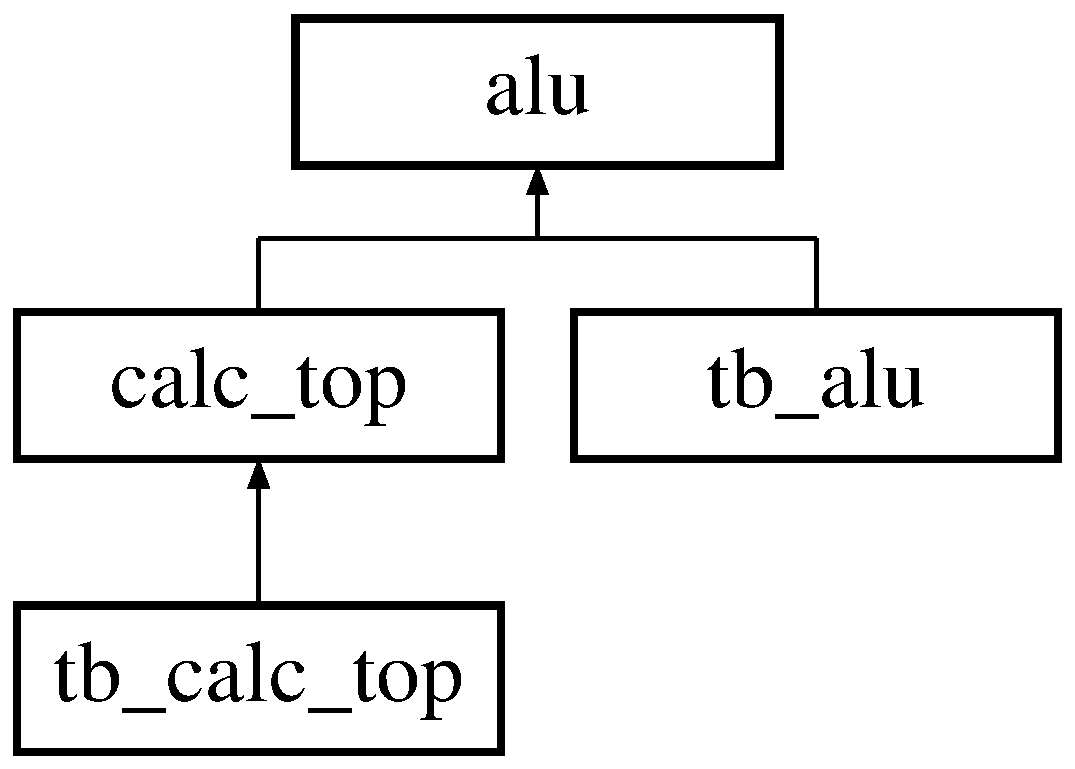
\includegraphics[height=3.000000cm]{classalu}
\end{center}
\end{figure}
\subsection*{Entities}
\begin{DoxyCompactItemize}
\item 
\hyperlink{classalu_1_1rtl}{rtl} architecture
\begin{DoxyCompactList}\small\item\em A\+LU Architecture R\+TL. \end{DoxyCompactList}\end{DoxyCompactItemize}
\subsection*{Libraries}
 \begin{DoxyCompactItemize}
\item 
\hyperlink{classalu_ae4f03c286607f3181e16b9aa12d0c6d4}{I\+E\+EE} 
\end{DoxyCompactItemize}
\subsection*{Use Clauses}
 \begin{DoxyCompactItemize}
\item 
\hyperlink{classalu_acd03516902501cd1c7296a98e22c6fcb}{std\+\_\+logic\+\_\+1164}   
\end{DoxyCompactItemize}
\subsection*{Ports}
 \begin{DoxyCompactItemize}
\item 
\hyperlink{classalu_abe949478e3f8aad0a6aeb1842fa6c608}{clk\+\_\+i}  {\bfseries {\bfseries \textcolor{keywordflow}{in}\textcolor{vhdlchar}{ }}} {\bfseries \textcolor{comment}{std\+\_\+logic}\textcolor{vhdlchar}{ }} 
\item 
\hyperlink{classalu_a55da7e76960757f8c6842e86a28ee7be}{reset\+\_\+i}  {\bfseries {\bfseries \textcolor{keywordflow}{in}\textcolor{vhdlchar}{ }}} {\bfseries \textcolor{comment}{std\+\_\+logic}\textcolor{vhdlchar}{ }} 
\item 
\hyperlink{classalu_a1127482098676cfc6ce7e98ba675ee27}{op1\+\_\+i}  {\bfseries {\bfseries \textcolor{keywordflow}{in}\textcolor{vhdlchar}{ }}} {\bfseries \textcolor{comment}{std\+\_\+logic\+\_\+vector}\textcolor{vhdlchar}{ }\textcolor{vhdlchar}{(}\textcolor{vhdlchar}{ }\textcolor{vhdlchar}{ } \textcolor{vhdldigit}{11} \textcolor{vhdlchar}{ }\textcolor{keywordflow}{downto}\textcolor{vhdlchar}{ }\textcolor{vhdlchar}{ } \textcolor{vhdldigit}{0} \textcolor{vhdlchar}{ }\textcolor{vhdlchar}{)}\textcolor{vhdlchar}{ }} 
\item 
\hyperlink{classalu_ae346648ed4ed2217b5e8d668b165aff2}{op2\+\_\+i}  {\bfseries {\bfseries \textcolor{keywordflow}{in}\textcolor{vhdlchar}{ }}} {\bfseries \textcolor{comment}{std\+\_\+logic\+\_\+vector}\textcolor{vhdlchar}{ }\textcolor{vhdlchar}{(}\textcolor{vhdlchar}{ }\textcolor{vhdlchar}{ } \textcolor{vhdldigit}{11} \textcolor{vhdlchar}{ }\textcolor{keywordflow}{downto}\textcolor{vhdlchar}{ }\textcolor{vhdlchar}{ } \textcolor{vhdldigit}{0} \textcolor{vhdlchar}{ }\textcolor{vhdlchar}{)}\textcolor{vhdlchar}{ }} 
\item 
\hyperlink{classalu_aee662ea38c86cd2e7dc1970ce8a6d5e9}{optype\+\_\+i}  {\bfseries {\bfseries \textcolor{keywordflow}{in}\textcolor{vhdlchar}{ }}} {\bfseries \textcolor{comment}{std\+\_\+logic\+\_\+vector}\textcolor{vhdlchar}{ }\textcolor{vhdlchar}{(}\textcolor{vhdlchar}{ }\textcolor{vhdlchar}{ } \textcolor{vhdldigit}{3} \textcolor{vhdlchar}{ }\textcolor{keywordflow}{downto}\textcolor{vhdlchar}{ }\textcolor{vhdlchar}{ } \textcolor{vhdldigit}{0} \textcolor{vhdlchar}{ }\textcolor{vhdlchar}{)}\textcolor{vhdlchar}{ }} 
\item 
\hyperlink{classalu_aba7911228d421cdfd5fc4eb74a60572c}{start\+\_\+i}  {\bfseries {\bfseries \textcolor{keywordflow}{in}\textcolor{vhdlchar}{ }}} {\bfseries \textcolor{comment}{std\+\_\+logic}\textcolor{vhdlchar}{ }} 
\item 
\hyperlink{classalu_a3e4609af33f8de496eb53352525eb9e7}{finished\+\_\+o}  {\bfseries {\bfseries \textcolor{keywordflow}{out}\textcolor{vhdlchar}{ }}} {\bfseries \textcolor{comment}{std\+\_\+logic}\textcolor{vhdlchar}{ }} 
\item 
\hyperlink{classalu_a4c4aa4e657b005516ee13f5b57054b9a}{result\+\_\+o}  {\bfseries {\bfseries \textcolor{keywordflow}{out}\textcolor{vhdlchar}{ }}} {\bfseries \textcolor{comment}{std\+\_\+logic\+\_\+vector}\textcolor{vhdlchar}{ }\textcolor{vhdlchar}{(}\textcolor{vhdlchar}{ }\textcolor{vhdlchar}{ } \textcolor{vhdldigit}{15} \textcolor{vhdlchar}{ }\textcolor{keywordflow}{downto}\textcolor{vhdlchar}{ }\textcolor{vhdlchar}{ } \textcolor{vhdldigit}{0} \textcolor{vhdlchar}{ }\textcolor{vhdlchar}{)}\textcolor{vhdlchar}{ }} 
\item 
\hyperlink{classalu_ad931fb1d7982869689b7072b46bf5f0b}{sign\+\_\+o}  {\bfseries {\bfseries \textcolor{keywordflow}{out}\textcolor{vhdlchar}{ }}} {\bfseries \textcolor{comment}{std\+\_\+logic}\textcolor{vhdlchar}{ }} 
\item 
\hyperlink{classalu_a7771d7a30216542931475a12593b972c}{overflow\+\_\+o}  {\bfseries {\bfseries \textcolor{keywordflow}{out}\textcolor{vhdlchar}{ }}} {\bfseries \textcolor{comment}{std\+\_\+logic}\textcolor{vhdlchar}{ }} 
\item 
\hyperlink{classalu_a43d3fe459020288f9fd3fe64782b7402}{error\+\_\+o}  {\bfseries {\bfseries \textcolor{keywordflow}{out}\textcolor{vhdlchar}{ }}} {\bfseries \textcolor{comment}{std\+\_\+logic}\textcolor{vhdlchar}{ }} 
\end{DoxyCompactItemize}


\subsection{Detailed Description}
A\+LU Entity. 

The A\+LU is part of the calculator project. 

\subsection{Member Data Documentation}
\mbox{\Hypertarget{classalu_abe949478e3f8aad0a6aeb1842fa6c608}\label{classalu_abe949478e3f8aad0a6aeb1842fa6c608}} 
\index{alu@{alu}!clk\+\_\+i@{clk\+\_\+i}}
\index{clk\+\_\+i@{clk\+\_\+i}!alu@{alu}}
\subsubsection{\texorpdfstring{clk\+\_\+i}{clk\_i}}
{\footnotesize\ttfamily \hyperlink{classalu_abe949478e3f8aad0a6aeb1842fa6c608}{clk\+\_\+i} {\bfseries \textcolor{keywordflow}{in}\textcolor{vhdlchar}{ }} {\bfseries \textcolor{comment}{std\+\_\+logic}\textcolor{vhdlchar}{ }} \hspace{0.3cm}{\ttfamily [Port]}}

\mbox{\Hypertarget{classalu_a43d3fe459020288f9fd3fe64782b7402}\label{classalu_a43d3fe459020288f9fd3fe64782b7402}} 
\index{alu@{alu}!error\+\_\+o@{error\+\_\+o}}
\index{error\+\_\+o@{error\+\_\+o}!alu@{alu}}
\subsubsection{\texorpdfstring{error\+\_\+o}{error\_o}}
{\footnotesize\ttfamily \hyperlink{classalu_a43d3fe459020288f9fd3fe64782b7402}{error\+\_\+o} {\bfseries \textcolor{keywordflow}{out}\textcolor{vhdlchar}{ }} {\bfseries \textcolor{comment}{std\+\_\+logic}\textcolor{vhdlchar}{ }} \hspace{0.3cm}{\ttfamily [Port]}}

\mbox{\Hypertarget{classalu_a3e4609af33f8de496eb53352525eb9e7}\label{classalu_a3e4609af33f8de496eb53352525eb9e7}} 
\index{alu@{alu}!finished\+\_\+o@{finished\+\_\+o}}
\index{finished\+\_\+o@{finished\+\_\+o}!alu@{alu}}
\subsubsection{\texorpdfstring{finished\+\_\+o}{finished\_o}}
{\footnotesize\ttfamily \hyperlink{classalu_a3e4609af33f8de496eb53352525eb9e7}{finished\+\_\+o} {\bfseries \textcolor{keywordflow}{out}\textcolor{vhdlchar}{ }} {\bfseries \textcolor{comment}{std\+\_\+logic}\textcolor{vhdlchar}{ }} \hspace{0.3cm}{\ttfamily [Port]}}

\mbox{\Hypertarget{classalu_ae4f03c286607f3181e16b9aa12d0c6d4}\label{classalu_ae4f03c286607f3181e16b9aa12d0c6d4}} 
\index{alu@{alu}!I\+E\+EE@{I\+E\+EE}}
\index{I\+E\+EE@{I\+E\+EE}!alu@{alu}}
\subsubsection{\texorpdfstring{I\+E\+EE}{IEEE}}
{\footnotesize\ttfamily \hyperlink{classalu_ae4f03c286607f3181e16b9aa12d0c6d4}{I\+E\+EE}\hspace{0.3cm}{\ttfamily [Library]}}

\mbox{\Hypertarget{classalu_a1127482098676cfc6ce7e98ba675ee27}\label{classalu_a1127482098676cfc6ce7e98ba675ee27}} 
\index{alu@{alu}!op1\+\_\+i@{op1\+\_\+i}}
\index{op1\+\_\+i@{op1\+\_\+i}!alu@{alu}}
\subsubsection{\texorpdfstring{op1\+\_\+i}{op1\_i}}
{\footnotesize\ttfamily \hyperlink{classalu_a1127482098676cfc6ce7e98ba675ee27}{op1\+\_\+i} {\bfseries \textcolor{keywordflow}{in}\textcolor{vhdlchar}{ }} {\bfseries \textcolor{comment}{std\+\_\+logic\+\_\+vector}\textcolor{vhdlchar}{ }\textcolor{vhdlchar}{(}\textcolor{vhdlchar}{ }\textcolor{vhdlchar}{ } \textcolor{vhdldigit}{11} \textcolor{vhdlchar}{ }\textcolor{keywordflow}{downto}\textcolor{vhdlchar}{ }\textcolor{vhdlchar}{ } \textcolor{vhdldigit}{0} \textcolor{vhdlchar}{ }\textcolor{vhdlchar}{)}\textcolor{vhdlchar}{ }} \hspace{0.3cm}{\ttfamily [Port]}}

\mbox{\Hypertarget{classalu_ae346648ed4ed2217b5e8d668b165aff2}\label{classalu_ae346648ed4ed2217b5e8d668b165aff2}} 
\index{alu@{alu}!op2\+\_\+i@{op2\+\_\+i}}
\index{op2\+\_\+i@{op2\+\_\+i}!alu@{alu}}
\subsubsection{\texorpdfstring{op2\+\_\+i}{op2\_i}}
{\footnotesize\ttfamily \hyperlink{classalu_ae346648ed4ed2217b5e8d668b165aff2}{op2\+\_\+i} {\bfseries \textcolor{keywordflow}{in}\textcolor{vhdlchar}{ }} {\bfseries \textcolor{comment}{std\+\_\+logic\+\_\+vector}\textcolor{vhdlchar}{ }\textcolor{vhdlchar}{(}\textcolor{vhdlchar}{ }\textcolor{vhdlchar}{ } \textcolor{vhdldigit}{11} \textcolor{vhdlchar}{ }\textcolor{keywordflow}{downto}\textcolor{vhdlchar}{ }\textcolor{vhdlchar}{ } \textcolor{vhdldigit}{0} \textcolor{vhdlchar}{ }\textcolor{vhdlchar}{)}\textcolor{vhdlchar}{ }} \hspace{0.3cm}{\ttfamily [Port]}}

\mbox{\Hypertarget{classalu_aee662ea38c86cd2e7dc1970ce8a6d5e9}\label{classalu_aee662ea38c86cd2e7dc1970ce8a6d5e9}} 
\index{alu@{alu}!optype\+\_\+i@{optype\+\_\+i}}
\index{optype\+\_\+i@{optype\+\_\+i}!alu@{alu}}
\subsubsection{\texorpdfstring{optype\+\_\+i}{optype\_i}}
{\footnotesize\ttfamily \hyperlink{classalu_aee662ea38c86cd2e7dc1970ce8a6d5e9}{optype\+\_\+i} {\bfseries \textcolor{keywordflow}{in}\textcolor{vhdlchar}{ }} {\bfseries \textcolor{comment}{std\+\_\+logic\+\_\+vector}\textcolor{vhdlchar}{ }\textcolor{vhdlchar}{(}\textcolor{vhdlchar}{ }\textcolor{vhdlchar}{ } \textcolor{vhdldigit}{3} \textcolor{vhdlchar}{ }\textcolor{keywordflow}{downto}\textcolor{vhdlchar}{ }\textcolor{vhdlchar}{ } \textcolor{vhdldigit}{0} \textcolor{vhdlchar}{ }\textcolor{vhdlchar}{)}\textcolor{vhdlchar}{ }} \hspace{0.3cm}{\ttfamily [Port]}}

\mbox{\Hypertarget{classalu_a7771d7a30216542931475a12593b972c}\label{classalu_a7771d7a30216542931475a12593b972c}} 
\index{alu@{alu}!overflow\+\_\+o@{overflow\+\_\+o}}
\index{overflow\+\_\+o@{overflow\+\_\+o}!alu@{alu}}
\subsubsection{\texorpdfstring{overflow\+\_\+o}{overflow\_o}}
{\footnotesize\ttfamily \hyperlink{classalu_a7771d7a30216542931475a12593b972c}{overflow\+\_\+o} {\bfseries \textcolor{keywordflow}{out}\textcolor{vhdlchar}{ }} {\bfseries \textcolor{comment}{std\+\_\+logic}\textcolor{vhdlchar}{ }} \hspace{0.3cm}{\ttfamily [Port]}}

\mbox{\Hypertarget{classalu_a55da7e76960757f8c6842e86a28ee7be}\label{classalu_a55da7e76960757f8c6842e86a28ee7be}} 
\index{alu@{alu}!reset\+\_\+i@{reset\+\_\+i}}
\index{reset\+\_\+i@{reset\+\_\+i}!alu@{alu}}
\subsubsection{\texorpdfstring{reset\+\_\+i}{reset\_i}}
{\footnotesize\ttfamily \hyperlink{classalu_a55da7e76960757f8c6842e86a28ee7be}{reset\+\_\+i} {\bfseries \textcolor{keywordflow}{in}\textcolor{vhdlchar}{ }} {\bfseries \textcolor{comment}{std\+\_\+logic}\textcolor{vhdlchar}{ }} \hspace{0.3cm}{\ttfamily [Port]}}

\mbox{\Hypertarget{classalu_a4c4aa4e657b005516ee13f5b57054b9a}\label{classalu_a4c4aa4e657b005516ee13f5b57054b9a}} 
\index{alu@{alu}!result\+\_\+o@{result\+\_\+o}}
\index{result\+\_\+o@{result\+\_\+o}!alu@{alu}}
\subsubsection{\texorpdfstring{result\+\_\+o}{result\_o}}
{\footnotesize\ttfamily \hyperlink{classalu_a4c4aa4e657b005516ee13f5b57054b9a}{result\+\_\+o} {\bfseries \textcolor{keywordflow}{out}\textcolor{vhdlchar}{ }} {\bfseries \textcolor{comment}{std\+\_\+logic\+\_\+vector}\textcolor{vhdlchar}{ }\textcolor{vhdlchar}{(}\textcolor{vhdlchar}{ }\textcolor{vhdlchar}{ } \textcolor{vhdldigit}{15} \textcolor{vhdlchar}{ }\textcolor{keywordflow}{downto}\textcolor{vhdlchar}{ }\textcolor{vhdlchar}{ } \textcolor{vhdldigit}{0} \textcolor{vhdlchar}{ }\textcolor{vhdlchar}{)}\textcolor{vhdlchar}{ }} \hspace{0.3cm}{\ttfamily [Port]}}

\mbox{\Hypertarget{classalu_ad931fb1d7982869689b7072b46bf5f0b}\label{classalu_ad931fb1d7982869689b7072b46bf5f0b}} 
\index{alu@{alu}!sign\+\_\+o@{sign\+\_\+o}}
\index{sign\+\_\+o@{sign\+\_\+o}!alu@{alu}}
\subsubsection{\texorpdfstring{sign\+\_\+o}{sign\_o}}
{\footnotesize\ttfamily \hyperlink{classalu_ad931fb1d7982869689b7072b46bf5f0b}{sign\+\_\+o} {\bfseries \textcolor{keywordflow}{out}\textcolor{vhdlchar}{ }} {\bfseries \textcolor{comment}{std\+\_\+logic}\textcolor{vhdlchar}{ }} \hspace{0.3cm}{\ttfamily [Port]}}

\mbox{\Hypertarget{classalu_aba7911228d421cdfd5fc4eb74a60572c}\label{classalu_aba7911228d421cdfd5fc4eb74a60572c}} 
\index{alu@{alu}!start\+\_\+i@{start\+\_\+i}}
\index{start\+\_\+i@{start\+\_\+i}!alu@{alu}}
\subsubsection{\texorpdfstring{start\+\_\+i}{start\_i}}
{\footnotesize\ttfamily \hyperlink{classalu_aba7911228d421cdfd5fc4eb74a60572c}{start\+\_\+i} {\bfseries \textcolor{keywordflow}{in}\textcolor{vhdlchar}{ }} {\bfseries \textcolor{comment}{std\+\_\+logic}\textcolor{vhdlchar}{ }} \hspace{0.3cm}{\ttfamily [Port]}}

\mbox{\Hypertarget{classalu_acd03516902501cd1c7296a98e22c6fcb}\label{classalu_acd03516902501cd1c7296a98e22c6fcb}} 
\index{alu@{alu}!std\+\_\+logic\+\_\+1164@{std\+\_\+logic\+\_\+1164}}
\index{std\+\_\+logic\+\_\+1164@{std\+\_\+logic\+\_\+1164}!alu@{alu}}
\subsubsection{\texorpdfstring{std\+\_\+logic\+\_\+1164}{std\_logic\_1164}}
{\footnotesize\ttfamily \hyperlink{classalu_acd03516902501cd1c7296a98e22c6fcb}{std\+\_\+logic\+\_\+1164}\hspace{0.3cm}{\ttfamily [Package]}}



The documentation for this class was generated from the following file\+:\begin{DoxyCompactItemize}
\item 
vhdl/\hyperlink{alu___8vhd}{alu\+\_\+.\+vhd}\end{DoxyCompactItemize}

\hypertarget{classcalc__ctrl}{}\section{calc\+\_\+ctrl Entity Reference}
\label{classcalc__ctrl}\index{calc\+\_\+ctrl@{calc\+\_\+ctrl}}


Calculator Control Unit Entity.  


Inheritance diagram for calc\+\_\+ctrl\+:\begin{figure}[H]
\begin{center}
\leavevmode
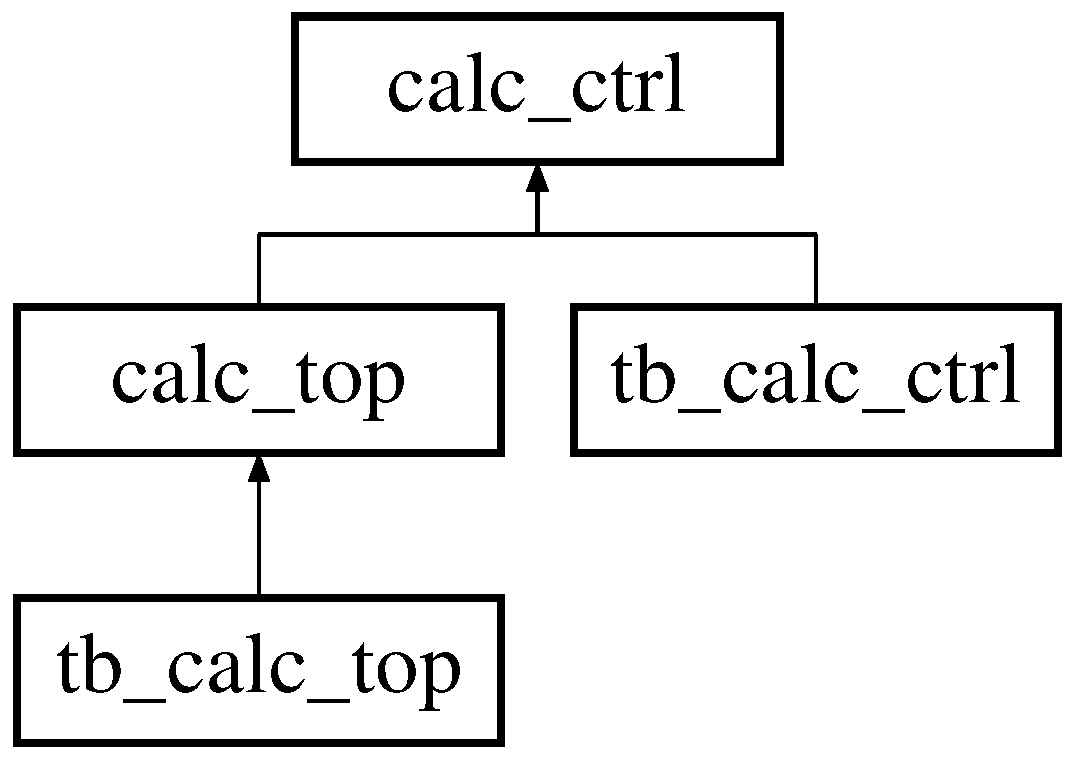
\includegraphics[height=3.000000cm]{classcalc__ctrl}
\end{center}
\end{figure}
\subsection*{Entities}
\begin{DoxyCompactItemize}
\item 
\hyperlink{classcalc__ctrl_1_1rtl}{rtl} architecture
\begin{DoxyCompactList}\small\item\em Calclator Control Unit Architecture R\+TL. \end{DoxyCompactList}\end{DoxyCompactItemize}
\subsection*{Libraries}
 \begin{DoxyCompactItemize}
\item 
\hyperlink{classcalc__ctrl_ae4f03c286607f3181e16b9aa12d0c6d4}{I\+E\+EE} 
\end{DoxyCompactItemize}
\subsection*{Use Clauses}
 \begin{DoxyCompactItemize}
\item 
\hyperlink{classcalc__ctrl_acd03516902501cd1c7296a98e22c6fcb}{std\+\_\+logic\+\_\+1164}   
\end{DoxyCompactItemize}
\subsection*{Ports}
 \begin{DoxyCompactItemize}
\item 
\hyperlink{classcalc__ctrl_abe949478e3f8aad0a6aeb1842fa6c608}{clk\+\_\+i}  {\bfseries {\bfseries \textcolor{keywordflow}{in}\textcolor{vhdlchar}{ }}} {\bfseries \textcolor{comment}{std\+\_\+logic}\textcolor{vhdlchar}{ }} 
\item 
\hyperlink{classcalc__ctrl_a55da7e76960757f8c6842e86a28ee7be}{reset\+\_\+i}  {\bfseries {\bfseries \textcolor{keywordflow}{in}\textcolor{vhdlchar}{ }}} {\bfseries \textcolor{comment}{std\+\_\+logic}\textcolor{vhdlchar}{ }} 
\item 
\hyperlink{classcalc__ctrl_a8f274a58bd077b3f0604e897f5fd8d06}{swsync\+\_\+i}  {\bfseries {\bfseries \textcolor{keywordflow}{in}\textcolor{vhdlchar}{ }}} {\bfseries \textcolor{comment}{std\+\_\+logic\+\_\+vector}\textcolor{vhdlchar}{ }\textcolor{vhdlchar}{(}\textcolor{vhdlchar}{ }\textcolor{vhdlchar}{ } \textcolor{vhdldigit}{15} \textcolor{vhdlchar}{ }\textcolor{keywordflow}{downto}\textcolor{vhdlchar}{ }\textcolor{vhdlchar}{ } \textcolor{vhdldigit}{0} \textcolor{vhdlchar}{ }\textcolor{vhdlchar}{)}\textcolor{vhdlchar}{ }} 
\item 
\hyperlink{classcalc__ctrl_ac9ed06cffb254d885992bb8fb780e8e6}{pbsync\+\_\+i}  {\bfseries {\bfseries \textcolor{keywordflow}{in}\textcolor{vhdlchar}{ }}} {\bfseries \textcolor{comment}{std\+\_\+logic\+\_\+vector}\textcolor{vhdlchar}{ }\textcolor{vhdlchar}{(}\textcolor{vhdlchar}{ }\textcolor{vhdlchar}{ } \textcolor{vhdldigit}{3} \textcolor{vhdlchar}{ }\textcolor{keywordflow}{downto}\textcolor{vhdlchar}{ }\textcolor{vhdlchar}{ } \textcolor{vhdldigit}{0} \textcolor{vhdlchar}{ }\textcolor{vhdlchar}{)}\textcolor{vhdlchar}{ }} 
\item 
\hyperlink{classcalc__ctrl_acaa48c495703015d6cbb2b40c0fd2e9b}{finished\+\_\+i}  {\bfseries {\bfseries \textcolor{keywordflow}{in}\textcolor{vhdlchar}{ }}} {\bfseries \textcolor{comment}{std\+\_\+logic}\textcolor{vhdlchar}{ }} 
\item 
\hyperlink{classcalc__ctrl_a58aeef44e9161ee5cb7cc149ac8ee71a}{result\+\_\+i}  {\bfseries {\bfseries \textcolor{keywordflow}{in}\textcolor{vhdlchar}{ }}} {\bfseries \textcolor{comment}{std\+\_\+logic\+\_\+vector}\textcolor{vhdlchar}{ }\textcolor{vhdlchar}{(}\textcolor{vhdlchar}{ }\textcolor{vhdlchar}{ } \textcolor{vhdldigit}{15} \textcolor{vhdlchar}{ }\textcolor{keywordflow}{downto}\textcolor{vhdlchar}{ }\textcolor{vhdlchar}{ } \textcolor{vhdldigit}{0} \textcolor{vhdlchar}{ }\textcolor{vhdlchar}{)}\textcolor{vhdlchar}{ }} 
\item 
\hyperlink{classcalc__ctrl_a36cce5b89625a8867788d2fddddd19fd}{sign\+\_\+i}  {\bfseries {\bfseries \textcolor{keywordflow}{in}\textcolor{vhdlchar}{ }}} {\bfseries \textcolor{comment}{std\+\_\+logic}\textcolor{vhdlchar}{ }} 
\item 
\hyperlink{classcalc__ctrl_a3844e90f5dc89f02aa3b92d8ca978cfd}{overflow\+\_\+i}  {\bfseries {\bfseries \textcolor{keywordflow}{in}\textcolor{vhdlchar}{ }}} {\bfseries \textcolor{comment}{std\+\_\+logic}\textcolor{vhdlchar}{ }} 
\item 
\hyperlink{classcalc__ctrl_a43d5e6363af801d5112bf95b65cf682a}{error\+\_\+i}  {\bfseries {\bfseries \textcolor{keywordflow}{in}\textcolor{vhdlchar}{ }}} {\bfseries \textcolor{comment}{std\+\_\+logic}\textcolor{vhdlchar}{ }} 
\item 
\hyperlink{classcalc__ctrl_ae2904ffa81e882d04f8595d84c2f8c9a}{dig0\+\_\+o}  {\bfseries {\bfseries \textcolor{keywordflow}{out}\textcolor{vhdlchar}{ }}} {\bfseries \textcolor{comment}{std\+\_\+logic\+\_\+vector}\textcolor{vhdlchar}{ }\textcolor{vhdlchar}{(}\textcolor{vhdlchar}{ }\textcolor{vhdlchar}{ } \textcolor{vhdldigit}{7} \textcolor{vhdlchar}{ }\textcolor{keywordflow}{downto}\textcolor{vhdlchar}{ }\textcolor{vhdlchar}{ } \textcolor{vhdldigit}{0} \textcolor{vhdlchar}{ }\textcolor{vhdlchar}{)}\textcolor{vhdlchar}{ }} 
\item 
\hyperlink{classcalc__ctrl_a30f5823bfbad17a9d14d0d3ac377d36f}{dig1\+\_\+o}  {\bfseries {\bfseries \textcolor{keywordflow}{out}\textcolor{vhdlchar}{ }}} {\bfseries \textcolor{comment}{std\+\_\+logic\+\_\+vector}\textcolor{vhdlchar}{ }\textcolor{vhdlchar}{(}\textcolor{vhdlchar}{ }\textcolor{vhdlchar}{ } \textcolor{vhdldigit}{7} \textcolor{vhdlchar}{ }\textcolor{keywordflow}{downto}\textcolor{vhdlchar}{ }\textcolor{vhdlchar}{ } \textcolor{vhdldigit}{0} \textcolor{vhdlchar}{ }\textcolor{vhdlchar}{)}\textcolor{vhdlchar}{ }} 
\item 
\hyperlink{classcalc__ctrl_a06ebb2808d498cfcb800e89ebfd6f06d}{dig2\+\_\+o}  {\bfseries {\bfseries \textcolor{keywordflow}{out}\textcolor{vhdlchar}{ }}} {\bfseries \textcolor{comment}{std\+\_\+logic\+\_\+vector}\textcolor{vhdlchar}{ }\textcolor{vhdlchar}{(}\textcolor{vhdlchar}{ }\textcolor{vhdlchar}{ } \textcolor{vhdldigit}{7} \textcolor{vhdlchar}{ }\textcolor{keywordflow}{downto}\textcolor{vhdlchar}{ }\textcolor{vhdlchar}{ } \textcolor{vhdldigit}{0} \textcolor{vhdlchar}{ }\textcolor{vhdlchar}{)}\textcolor{vhdlchar}{ }} 
\item 
\hyperlink{classcalc__ctrl_ad67620f795b122d474fbe00607b06702}{dig3\+\_\+o}  {\bfseries {\bfseries \textcolor{keywordflow}{out}\textcolor{vhdlchar}{ }}} {\bfseries \textcolor{comment}{std\+\_\+logic\+\_\+vector}\textcolor{vhdlchar}{ }\textcolor{vhdlchar}{(}\textcolor{vhdlchar}{ }\textcolor{vhdlchar}{ } \textcolor{vhdldigit}{7} \textcolor{vhdlchar}{ }\textcolor{keywordflow}{downto}\textcolor{vhdlchar}{ }\textcolor{vhdlchar}{ } \textcolor{vhdldigit}{0} \textcolor{vhdlchar}{ }\textcolor{vhdlchar}{)}\textcolor{vhdlchar}{ }} 
\item 
\hyperlink{classcalc__ctrl_ae622b8b55ca985e4965d79aab895a746}{led\+\_\+o}  {\bfseries {\bfseries \textcolor{keywordflow}{out}\textcolor{vhdlchar}{ }}} {\bfseries \textcolor{comment}{std\+\_\+logic\+\_\+vector}\textcolor{vhdlchar}{ }\textcolor{vhdlchar}{(}\textcolor{vhdlchar}{ }\textcolor{vhdlchar}{ } \textcolor{vhdldigit}{15} \textcolor{vhdlchar}{ }\textcolor{keywordflow}{downto}\textcolor{vhdlchar}{ }\textcolor{vhdlchar}{ } \textcolor{vhdldigit}{0} \textcolor{vhdlchar}{ }\textcolor{vhdlchar}{)}\textcolor{vhdlchar}{ }} 
\item 
\hyperlink{classcalc__ctrl_aa36aff52ea4782ad62fe55a5b35bfcb9}{op1\+\_\+o}  {\bfseries {\bfseries \textcolor{keywordflow}{out}\textcolor{vhdlchar}{ }}} {\bfseries \textcolor{comment}{std\+\_\+logic\+\_\+vector}\textcolor{vhdlchar}{ }\textcolor{vhdlchar}{(}\textcolor{vhdlchar}{ }\textcolor{vhdlchar}{ } \textcolor{vhdldigit}{11} \textcolor{vhdlchar}{ }\textcolor{keywordflow}{downto}\textcolor{vhdlchar}{ }\textcolor{vhdlchar}{ } \textcolor{vhdldigit}{0} \textcolor{vhdlchar}{ }\textcolor{vhdlchar}{)}\textcolor{vhdlchar}{ }} 
\item 
\hyperlink{classcalc__ctrl_ac5c54f5b95615dd2de14375f17f4ad4e}{op2\+\_\+o}  {\bfseries {\bfseries \textcolor{keywordflow}{out}\textcolor{vhdlchar}{ }}} {\bfseries \textcolor{comment}{std\+\_\+logic\+\_\+vector}\textcolor{vhdlchar}{ }\textcolor{vhdlchar}{(}\textcolor{vhdlchar}{ }\textcolor{vhdlchar}{ } \textcolor{vhdldigit}{11} \textcolor{vhdlchar}{ }\textcolor{keywordflow}{downto}\textcolor{vhdlchar}{ }\textcolor{vhdlchar}{ } \textcolor{vhdldigit}{0} \textcolor{vhdlchar}{ }\textcolor{vhdlchar}{)}\textcolor{vhdlchar}{ }} 
\item 
\hyperlink{classcalc__ctrl_af76d14ea083de87ece0fb97784b21ffc}{optype\+\_\+o}  {\bfseries {\bfseries \textcolor{keywordflow}{out}\textcolor{vhdlchar}{ }}} {\bfseries \textcolor{comment}{std\+\_\+logic\+\_\+vector}\textcolor{vhdlchar}{ }\textcolor{vhdlchar}{(}\textcolor{vhdlchar}{ }\textcolor{vhdlchar}{ } \textcolor{vhdldigit}{3} \textcolor{vhdlchar}{ }\textcolor{keywordflow}{downto}\textcolor{vhdlchar}{ }\textcolor{vhdlchar}{ } \textcolor{vhdldigit}{0} \textcolor{vhdlchar}{ }\textcolor{vhdlchar}{)}\textcolor{vhdlchar}{ }} 
\item 
\hyperlink{classcalc__ctrl_a6668aebe332a7b7161887353bd928a5b}{start\+\_\+o}  {\bfseries {\bfseries \textcolor{keywordflow}{out}\textcolor{vhdlchar}{ }}} {\bfseries \textcolor{comment}{std\+\_\+logic}\textcolor{vhdlchar}{ }} 
\end{DoxyCompactItemize}


\subsection{Detailed Description}
Calculator Control Unit Entity. 

The Calculator Control unit is part of the calculator project. 

\subsection{Member Data Documentation}
\mbox{\Hypertarget{classcalc__ctrl_abe949478e3f8aad0a6aeb1842fa6c608}\label{classcalc__ctrl_abe949478e3f8aad0a6aeb1842fa6c608}} 
\index{calc\+\_\+ctrl@{calc\+\_\+ctrl}!clk\+\_\+i@{clk\+\_\+i}}
\index{clk\+\_\+i@{clk\+\_\+i}!calc\+\_\+ctrl@{calc\+\_\+ctrl}}
\subsubsection{\texorpdfstring{clk\+\_\+i}{clk\_i}}
{\footnotesize\ttfamily \hyperlink{classcalc__ctrl_abe949478e3f8aad0a6aeb1842fa6c608}{clk\+\_\+i} {\bfseries \textcolor{keywordflow}{in}\textcolor{vhdlchar}{ }} {\bfseries \textcolor{comment}{std\+\_\+logic}\textcolor{vhdlchar}{ }} \hspace{0.3cm}{\ttfamily [Port]}}

\mbox{\Hypertarget{classcalc__ctrl_ae2904ffa81e882d04f8595d84c2f8c9a}\label{classcalc__ctrl_ae2904ffa81e882d04f8595d84c2f8c9a}} 
\index{calc\+\_\+ctrl@{calc\+\_\+ctrl}!dig0\+\_\+o@{dig0\+\_\+o}}
\index{dig0\+\_\+o@{dig0\+\_\+o}!calc\+\_\+ctrl@{calc\+\_\+ctrl}}
\subsubsection{\texorpdfstring{dig0\+\_\+o}{dig0\_o}}
{\footnotesize\ttfamily \hyperlink{classcalc__ctrl_ae2904ffa81e882d04f8595d84c2f8c9a}{dig0\+\_\+o} {\bfseries \textcolor{keywordflow}{out}\textcolor{vhdlchar}{ }} {\bfseries \textcolor{comment}{std\+\_\+logic\+\_\+vector}\textcolor{vhdlchar}{ }\textcolor{vhdlchar}{(}\textcolor{vhdlchar}{ }\textcolor{vhdlchar}{ } \textcolor{vhdldigit}{7} \textcolor{vhdlchar}{ }\textcolor{keywordflow}{downto}\textcolor{vhdlchar}{ }\textcolor{vhdlchar}{ } \textcolor{vhdldigit}{0} \textcolor{vhdlchar}{ }\textcolor{vhdlchar}{)}\textcolor{vhdlchar}{ }} \hspace{0.3cm}{\ttfamily [Port]}}

\mbox{\Hypertarget{classcalc__ctrl_a30f5823bfbad17a9d14d0d3ac377d36f}\label{classcalc__ctrl_a30f5823bfbad17a9d14d0d3ac377d36f}} 
\index{calc\+\_\+ctrl@{calc\+\_\+ctrl}!dig1\+\_\+o@{dig1\+\_\+o}}
\index{dig1\+\_\+o@{dig1\+\_\+o}!calc\+\_\+ctrl@{calc\+\_\+ctrl}}
\subsubsection{\texorpdfstring{dig1\+\_\+o}{dig1\_o}}
{\footnotesize\ttfamily \hyperlink{classcalc__ctrl_a30f5823bfbad17a9d14d0d3ac377d36f}{dig1\+\_\+o} {\bfseries \textcolor{keywordflow}{out}\textcolor{vhdlchar}{ }} {\bfseries \textcolor{comment}{std\+\_\+logic\+\_\+vector}\textcolor{vhdlchar}{ }\textcolor{vhdlchar}{(}\textcolor{vhdlchar}{ }\textcolor{vhdlchar}{ } \textcolor{vhdldigit}{7} \textcolor{vhdlchar}{ }\textcolor{keywordflow}{downto}\textcolor{vhdlchar}{ }\textcolor{vhdlchar}{ } \textcolor{vhdldigit}{0} \textcolor{vhdlchar}{ }\textcolor{vhdlchar}{)}\textcolor{vhdlchar}{ }} \hspace{0.3cm}{\ttfamily [Port]}}

\mbox{\Hypertarget{classcalc__ctrl_a06ebb2808d498cfcb800e89ebfd6f06d}\label{classcalc__ctrl_a06ebb2808d498cfcb800e89ebfd6f06d}} 
\index{calc\+\_\+ctrl@{calc\+\_\+ctrl}!dig2\+\_\+o@{dig2\+\_\+o}}
\index{dig2\+\_\+o@{dig2\+\_\+o}!calc\+\_\+ctrl@{calc\+\_\+ctrl}}
\subsubsection{\texorpdfstring{dig2\+\_\+o}{dig2\_o}}
{\footnotesize\ttfamily \hyperlink{classcalc__ctrl_a06ebb2808d498cfcb800e89ebfd6f06d}{dig2\+\_\+o} {\bfseries \textcolor{keywordflow}{out}\textcolor{vhdlchar}{ }} {\bfseries \textcolor{comment}{std\+\_\+logic\+\_\+vector}\textcolor{vhdlchar}{ }\textcolor{vhdlchar}{(}\textcolor{vhdlchar}{ }\textcolor{vhdlchar}{ } \textcolor{vhdldigit}{7} \textcolor{vhdlchar}{ }\textcolor{keywordflow}{downto}\textcolor{vhdlchar}{ }\textcolor{vhdlchar}{ } \textcolor{vhdldigit}{0} \textcolor{vhdlchar}{ }\textcolor{vhdlchar}{)}\textcolor{vhdlchar}{ }} \hspace{0.3cm}{\ttfamily [Port]}}

\mbox{\Hypertarget{classcalc__ctrl_ad67620f795b122d474fbe00607b06702}\label{classcalc__ctrl_ad67620f795b122d474fbe00607b06702}} 
\index{calc\+\_\+ctrl@{calc\+\_\+ctrl}!dig3\+\_\+o@{dig3\+\_\+o}}
\index{dig3\+\_\+o@{dig3\+\_\+o}!calc\+\_\+ctrl@{calc\+\_\+ctrl}}
\subsubsection{\texorpdfstring{dig3\+\_\+o}{dig3\_o}}
{\footnotesize\ttfamily \hyperlink{classcalc__ctrl_ad67620f795b122d474fbe00607b06702}{dig3\+\_\+o} {\bfseries \textcolor{keywordflow}{out}\textcolor{vhdlchar}{ }} {\bfseries \textcolor{comment}{std\+\_\+logic\+\_\+vector}\textcolor{vhdlchar}{ }\textcolor{vhdlchar}{(}\textcolor{vhdlchar}{ }\textcolor{vhdlchar}{ } \textcolor{vhdldigit}{7} \textcolor{vhdlchar}{ }\textcolor{keywordflow}{downto}\textcolor{vhdlchar}{ }\textcolor{vhdlchar}{ } \textcolor{vhdldigit}{0} \textcolor{vhdlchar}{ }\textcolor{vhdlchar}{)}\textcolor{vhdlchar}{ }} \hspace{0.3cm}{\ttfamily [Port]}}

\mbox{\Hypertarget{classcalc__ctrl_a43d5e6363af801d5112bf95b65cf682a}\label{classcalc__ctrl_a43d5e6363af801d5112bf95b65cf682a}} 
\index{calc\+\_\+ctrl@{calc\+\_\+ctrl}!error\+\_\+i@{error\+\_\+i}}
\index{error\+\_\+i@{error\+\_\+i}!calc\+\_\+ctrl@{calc\+\_\+ctrl}}
\subsubsection{\texorpdfstring{error\+\_\+i}{error\_i}}
{\footnotesize\ttfamily \hyperlink{classcalc__ctrl_a43d5e6363af801d5112bf95b65cf682a}{error\+\_\+i} {\bfseries \textcolor{keywordflow}{in}\textcolor{vhdlchar}{ }} {\bfseries \textcolor{comment}{std\+\_\+logic}\textcolor{vhdlchar}{ }} \hspace{0.3cm}{\ttfamily [Port]}}

\mbox{\Hypertarget{classcalc__ctrl_acaa48c495703015d6cbb2b40c0fd2e9b}\label{classcalc__ctrl_acaa48c495703015d6cbb2b40c0fd2e9b}} 
\index{calc\+\_\+ctrl@{calc\+\_\+ctrl}!finished\+\_\+i@{finished\+\_\+i}}
\index{finished\+\_\+i@{finished\+\_\+i}!calc\+\_\+ctrl@{calc\+\_\+ctrl}}
\subsubsection{\texorpdfstring{finished\+\_\+i}{finished\_i}}
{\footnotesize\ttfamily \hyperlink{classcalc__ctrl_acaa48c495703015d6cbb2b40c0fd2e9b}{finished\+\_\+i} {\bfseries \textcolor{keywordflow}{in}\textcolor{vhdlchar}{ }} {\bfseries \textcolor{comment}{std\+\_\+logic}\textcolor{vhdlchar}{ }} \hspace{0.3cm}{\ttfamily [Port]}}

\mbox{\Hypertarget{classcalc__ctrl_ae4f03c286607f3181e16b9aa12d0c6d4}\label{classcalc__ctrl_ae4f03c286607f3181e16b9aa12d0c6d4}} 
\index{calc\+\_\+ctrl@{calc\+\_\+ctrl}!I\+E\+EE@{I\+E\+EE}}
\index{I\+E\+EE@{I\+E\+EE}!calc\+\_\+ctrl@{calc\+\_\+ctrl}}
\subsubsection{\texorpdfstring{I\+E\+EE}{IEEE}}
{\footnotesize\ttfamily \hyperlink{classcalc__ctrl_ae4f03c286607f3181e16b9aa12d0c6d4}{I\+E\+EE}\hspace{0.3cm}{\ttfamily [Library]}}

\mbox{\Hypertarget{classcalc__ctrl_ae622b8b55ca985e4965d79aab895a746}\label{classcalc__ctrl_ae622b8b55ca985e4965d79aab895a746}} 
\index{calc\+\_\+ctrl@{calc\+\_\+ctrl}!led\+\_\+o@{led\+\_\+o}}
\index{led\+\_\+o@{led\+\_\+o}!calc\+\_\+ctrl@{calc\+\_\+ctrl}}
\subsubsection{\texorpdfstring{led\+\_\+o}{led\_o}}
{\footnotesize\ttfamily \hyperlink{classcalc__ctrl_ae622b8b55ca985e4965d79aab895a746}{led\+\_\+o} {\bfseries \textcolor{keywordflow}{out}\textcolor{vhdlchar}{ }} {\bfseries \textcolor{comment}{std\+\_\+logic\+\_\+vector}\textcolor{vhdlchar}{ }\textcolor{vhdlchar}{(}\textcolor{vhdlchar}{ }\textcolor{vhdlchar}{ } \textcolor{vhdldigit}{15} \textcolor{vhdlchar}{ }\textcolor{keywordflow}{downto}\textcolor{vhdlchar}{ }\textcolor{vhdlchar}{ } \textcolor{vhdldigit}{0} \textcolor{vhdlchar}{ }\textcolor{vhdlchar}{)}\textcolor{vhdlchar}{ }} \hspace{0.3cm}{\ttfamily [Port]}}

\mbox{\Hypertarget{classcalc__ctrl_aa36aff52ea4782ad62fe55a5b35bfcb9}\label{classcalc__ctrl_aa36aff52ea4782ad62fe55a5b35bfcb9}} 
\index{calc\+\_\+ctrl@{calc\+\_\+ctrl}!op1\+\_\+o@{op1\+\_\+o}}
\index{op1\+\_\+o@{op1\+\_\+o}!calc\+\_\+ctrl@{calc\+\_\+ctrl}}
\subsubsection{\texorpdfstring{op1\+\_\+o}{op1\_o}}
{\footnotesize\ttfamily \hyperlink{classcalc__ctrl_aa36aff52ea4782ad62fe55a5b35bfcb9}{op1\+\_\+o} {\bfseries \textcolor{keywordflow}{out}\textcolor{vhdlchar}{ }} {\bfseries \textcolor{comment}{std\+\_\+logic\+\_\+vector}\textcolor{vhdlchar}{ }\textcolor{vhdlchar}{(}\textcolor{vhdlchar}{ }\textcolor{vhdlchar}{ } \textcolor{vhdldigit}{11} \textcolor{vhdlchar}{ }\textcolor{keywordflow}{downto}\textcolor{vhdlchar}{ }\textcolor{vhdlchar}{ } \textcolor{vhdldigit}{0} \textcolor{vhdlchar}{ }\textcolor{vhdlchar}{)}\textcolor{vhdlchar}{ }} \hspace{0.3cm}{\ttfamily [Port]}}

\mbox{\Hypertarget{classcalc__ctrl_ac5c54f5b95615dd2de14375f17f4ad4e}\label{classcalc__ctrl_ac5c54f5b95615dd2de14375f17f4ad4e}} 
\index{calc\+\_\+ctrl@{calc\+\_\+ctrl}!op2\+\_\+o@{op2\+\_\+o}}
\index{op2\+\_\+o@{op2\+\_\+o}!calc\+\_\+ctrl@{calc\+\_\+ctrl}}
\subsubsection{\texorpdfstring{op2\+\_\+o}{op2\_o}}
{\footnotesize\ttfamily \hyperlink{classcalc__ctrl_ac5c54f5b95615dd2de14375f17f4ad4e}{op2\+\_\+o} {\bfseries \textcolor{keywordflow}{out}\textcolor{vhdlchar}{ }} {\bfseries \textcolor{comment}{std\+\_\+logic\+\_\+vector}\textcolor{vhdlchar}{ }\textcolor{vhdlchar}{(}\textcolor{vhdlchar}{ }\textcolor{vhdlchar}{ } \textcolor{vhdldigit}{11} \textcolor{vhdlchar}{ }\textcolor{keywordflow}{downto}\textcolor{vhdlchar}{ }\textcolor{vhdlchar}{ } \textcolor{vhdldigit}{0} \textcolor{vhdlchar}{ }\textcolor{vhdlchar}{)}\textcolor{vhdlchar}{ }} \hspace{0.3cm}{\ttfamily [Port]}}

\mbox{\Hypertarget{classcalc__ctrl_af76d14ea083de87ece0fb97784b21ffc}\label{classcalc__ctrl_af76d14ea083de87ece0fb97784b21ffc}} 
\index{calc\+\_\+ctrl@{calc\+\_\+ctrl}!optype\+\_\+o@{optype\+\_\+o}}
\index{optype\+\_\+o@{optype\+\_\+o}!calc\+\_\+ctrl@{calc\+\_\+ctrl}}
\subsubsection{\texorpdfstring{optype\+\_\+o}{optype\_o}}
{\footnotesize\ttfamily \hyperlink{classcalc__ctrl_af76d14ea083de87ece0fb97784b21ffc}{optype\+\_\+o} {\bfseries \textcolor{keywordflow}{out}\textcolor{vhdlchar}{ }} {\bfseries \textcolor{comment}{std\+\_\+logic\+\_\+vector}\textcolor{vhdlchar}{ }\textcolor{vhdlchar}{(}\textcolor{vhdlchar}{ }\textcolor{vhdlchar}{ } \textcolor{vhdldigit}{3} \textcolor{vhdlchar}{ }\textcolor{keywordflow}{downto}\textcolor{vhdlchar}{ }\textcolor{vhdlchar}{ } \textcolor{vhdldigit}{0} \textcolor{vhdlchar}{ }\textcolor{vhdlchar}{)}\textcolor{vhdlchar}{ }} \hspace{0.3cm}{\ttfamily [Port]}}

\mbox{\Hypertarget{classcalc__ctrl_a3844e90f5dc89f02aa3b92d8ca978cfd}\label{classcalc__ctrl_a3844e90f5dc89f02aa3b92d8ca978cfd}} 
\index{calc\+\_\+ctrl@{calc\+\_\+ctrl}!overflow\+\_\+i@{overflow\+\_\+i}}
\index{overflow\+\_\+i@{overflow\+\_\+i}!calc\+\_\+ctrl@{calc\+\_\+ctrl}}
\subsubsection{\texorpdfstring{overflow\+\_\+i}{overflow\_i}}
{\footnotesize\ttfamily \hyperlink{classcalc__ctrl_a3844e90f5dc89f02aa3b92d8ca978cfd}{overflow\+\_\+i} {\bfseries \textcolor{keywordflow}{in}\textcolor{vhdlchar}{ }} {\bfseries \textcolor{comment}{std\+\_\+logic}\textcolor{vhdlchar}{ }} \hspace{0.3cm}{\ttfamily [Port]}}

\mbox{\Hypertarget{classcalc__ctrl_ac9ed06cffb254d885992bb8fb780e8e6}\label{classcalc__ctrl_ac9ed06cffb254d885992bb8fb780e8e6}} 
\index{calc\+\_\+ctrl@{calc\+\_\+ctrl}!pbsync\+\_\+i@{pbsync\+\_\+i}}
\index{pbsync\+\_\+i@{pbsync\+\_\+i}!calc\+\_\+ctrl@{calc\+\_\+ctrl}}
\subsubsection{\texorpdfstring{pbsync\+\_\+i}{pbsync\_i}}
{\footnotesize\ttfamily \hyperlink{classcalc__ctrl_ac9ed06cffb254d885992bb8fb780e8e6}{pbsync\+\_\+i} {\bfseries \textcolor{keywordflow}{in}\textcolor{vhdlchar}{ }} {\bfseries \textcolor{comment}{std\+\_\+logic\+\_\+vector}\textcolor{vhdlchar}{ }\textcolor{vhdlchar}{(}\textcolor{vhdlchar}{ }\textcolor{vhdlchar}{ } \textcolor{vhdldigit}{3} \textcolor{vhdlchar}{ }\textcolor{keywordflow}{downto}\textcolor{vhdlchar}{ }\textcolor{vhdlchar}{ } \textcolor{vhdldigit}{0} \textcolor{vhdlchar}{ }\textcolor{vhdlchar}{)}\textcolor{vhdlchar}{ }} \hspace{0.3cm}{\ttfamily [Port]}}

\mbox{\Hypertarget{classcalc__ctrl_a55da7e76960757f8c6842e86a28ee7be}\label{classcalc__ctrl_a55da7e76960757f8c6842e86a28ee7be}} 
\index{calc\+\_\+ctrl@{calc\+\_\+ctrl}!reset\+\_\+i@{reset\+\_\+i}}
\index{reset\+\_\+i@{reset\+\_\+i}!calc\+\_\+ctrl@{calc\+\_\+ctrl}}
\subsubsection{\texorpdfstring{reset\+\_\+i}{reset\_i}}
{\footnotesize\ttfamily \hyperlink{classcalc__ctrl_a55da7e76960757f8c6842e86a28ee7be}{reset\+\_\+i} {\bfseries \textcolor{keywordflow}{in}\textcolor{vhdlchar}{ }} {\bfseries \textcolor{comment}{std\+\_\+logic}\textcolor{vhdlchar}{ }} \hspace{0.3cm}{\ttfamily [Port]}}

\mbox{\Hypertarget{classcalc__ctrl_a58aeef44e9161ee5cb7cc149ac8ee71a}\label{classcalc__ctrl_a58aeef44e9161ee5cb7cc149ac8ee71a}} 
\index{calc\+\_\+ctrl@{calc\+\_\+ctrl}!result\+\_\+i@{result\+\_\+i}}
\index{result\+\_\+i@{result\+\_\+i}!calc\+\_\+ctrl@{calc\+\_\+ctrl}}
\subsubsection{\texorpdfstring{result\+\_\+i}{result\_i}}
{\footnotesize\ttfamily \hyperlink{classcalc__ctrl_a58aeef44e9161ee5cb7cc149ac8ee71a}{result\+\_\+i} {\bfseries \textcolor{keywordflow}{in}\textcolor{vhdlchar}{ }} {\bfseries \textcolor{comment}{std\+\_\+logic\+\_\+vector}\textcolor{vhdlchar}{ }\textcolor{vhdlchar}{(}\textcolor{vhdlchar}{ }\textcolor{vhdlchar}{ } \textcolor{vhdldigit}{15} \textcolor{vhdlchar}{ }\textcolor{keywordflow}{downto}\textcolor{vhdlchar}{ }\textcolor{vhdlchar}{ } \textcolor{vhdldigit}{0} \textcolor{vhdlchar}{ }\textcolor{vhdlchar}{)}\textcolor{vhdlchar}{ }} \hspace{0.3cm}{\ttfamily [Port]}}

\mbox{\Hypertarget{classcalc__ctrl_a36cce5b89625a8867788d2fddddd19fd}\label{classcalc__ctrl_a36cce5b89625a8867788d2fddddd19fd}} 
\index{calc\+\_\+ctrl@{calc\+\_\+ctrl}!sign\+\_\+i@{sign\+\_\+i}}
\index{sign\+\_\+i@{sign\+\_\+i}!calc\+\_\+ctrl@{calc\+\_\+ctrl}}
\subsubsection{\texorpdfstring{sign\+\_\+i}{sign\_i}}
{\footnotesize\ttfamily \hyperlink{classcalc__ctrl_a36cce5b89625a8867788d2fddddd19fd}{sign\+\_\+i} {\bfseries \textcolor{keywordflow}{in}\textcolor{vhdlchar}{ }} {\bfseries \textcolor{comment}{std\+\_\+logic}\textcolor{vhdlchar}{ }} \hspace{0.3cm}{\ttfamily [Port]}}

\mbox{\Hypertarget{classcalc__ctrl_a6668aebe332a7b7161887353bd928a5b}\label{classcalc__ctrl_a6668aebe332a7b7161887353bd928a5b}} 
\index{calc\+\_\+ctrl@{calc\+\_\+ctrl}!start\+\_\+o@{start\+\_\+o}}
\index{start\+\_\+o@{start\+\_\+o}!calc\+\_\+ctrl@{calc\+\_\+ctrl}}
\subsubsection{\texorpdfstring{start\+\_\+o}{start\_o}}
{\footnotesize\ttfamily \hyperlink{classcalc__ctrl_a6668aebe332a7b7161887353bd928a5b}{start\+\_\+o} {\bfseries \textcolor{keywordflow}{out}\textcolor{vhdlchar}{ }} {\bfseries \textcolor{comment}{std\+\_\+logic}\textcolor{vhdlchar}{ }} \hspace{0.3cm}{\ttfamily [Port]}}

\mbox{\Hypertarget{classcalc__ctrl_acd03516902501cd1c7296a98e22c6fcb}\label{classcalc__ctrl_acd03516902501cd1c7296a98e22c6fcb}} 
\index{calc\+\_\+ctrl@{calc\+\_\+ctrl}!std\+\_\+logic\+\_\+1164@{std\+\_\+logic\+\_\+1164}}
\index{std\+\_\+logic\+\_\+1164@{std\+\_\+logic\+\_\+1164}!calc\+\_\+ctrl@{calc\+\_\+ctrl}}
\subsubsection{\texorpdfstring{std\+\_\+logic\+\_\+1164}{std\_logic\_1164}}
{\footnotesize\ttfamily \hyperlink{classcalc__ctrl_acd03516902501cd1c7296a98e22c6fcb}{std\+\_\+logic\+\_\+1164}\hspace{0.3cm}{\ttfamily [Package]}}

\mbox{\Hypertarget{classcalc__ctrl_a8f274a58bd077b3f0604e897f5fd8d06}\label{classcalc__ctrl_a8f274a58bd077b3f0604e897f5fd8d06}} 
\index{calc\+\_\+ctrl@{calc\+\_\+ctrl}!swsync\+\_\+i@{swsync\+\_\+i}}
\index{swsync\+\_\+i@{swsync\+\_\+i}!calc\+\_\+ctrl@{calc\+\_\+ctrl}}
\subsubsection{\texorpdfstring{swsync\+\_\+i}{swsync\_i}}
{\footnotesize\ttfamily \hyperlink{classcalc__ctrl_a8f274a58bd077b3f0604e897f5fd8d06}{swsync\+\_\+i} {\bfseries \textcolor{keywordflow}{in}\textcolor{vhdlchar}{ }} {\bfseries \textcolor{comment}{std\+\_\+logic\+\_\+vector}\textcolor{vhdlchar}{ }\textcolor{vhdlchar}{(}\textcolor{vhdlchar}{ }\textcolor{vhdlchar}{ } \textcolor{vhdldigit}{15} \textcolor{vhdlchar}{ }\textcolor{keywordflow}{downto}\textcolor{vhdlchar}{ }\textcolor{vhdlchar}{ } \textcolor{vhdldigit}{0} \textcolor{vhdlchar}{ }\textcolor{vhdlchar}{)}\textcolor{vhdlchar}{ }} \hspace{0.3cm}{\ttfamily [Port]}}



The documentation for this class was generated from the following file\+:\begin{DoxyCompactItemize}
\item 
vhdl/\hyperlink{calc__ctrl___8vhd}{calc\+\_\+ctrl\+\_\+.\+vhd}\end{DoxyCompactItemize}

\hypertarget{classcalc__top}{}\section{calc\+\_\+top Entity Reference}
\label{classcalc__top}\index{calc\+\_\+top@{calc\+\_\+top}}


Calculator Top Design Entity.  


Inheritance diagram for calc\+\_\+top\+:\begin{figure}[H]
\begin{center}
\leavevmode
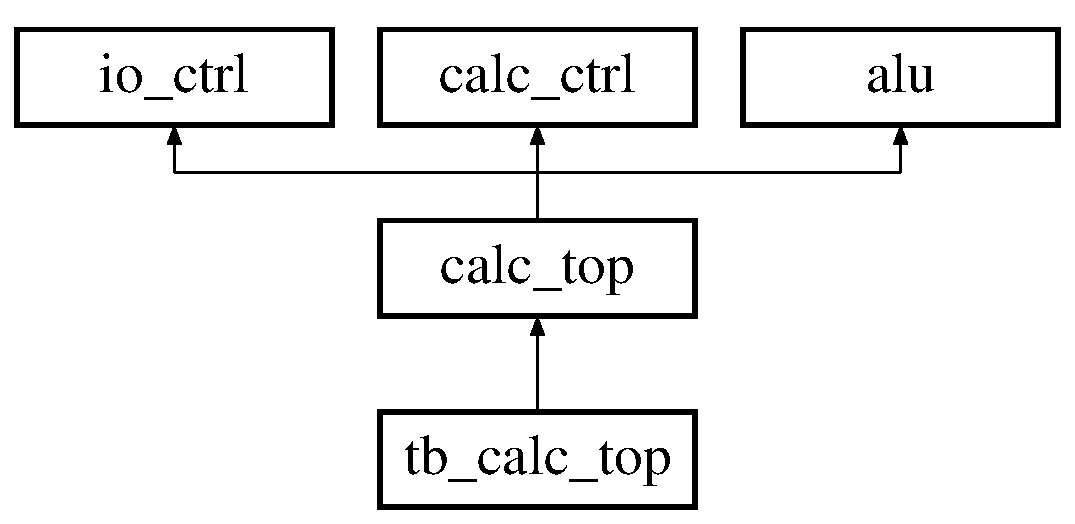
\includegraphics[height=3.000000cm]{classcalc__top}
\end{center}
\end{figure}
\subsection*{Entities}
\begin{DoxyCompactItemize}
\item 
\hyperlink{classcalc__top_1_1struc}{struc} architecture
\begin{DoxyCompactList}\small\item\em Calculator Top Architecture R\+T\+L-\/\+S\+T\+R\+UC. \end{DoxyCompactList}\end{DoxyCompactItemize}
\subsection*{Libraries}
 \begin{DoxyCompactItemize}
\item 
\hyperlink{classcalc__top_ae4f03c286607f3181e16b9aa12d0c6d4}{I\+E\+EE} 
\end{DoxyCompactItemize}
\subsection*{Use Clauses}
 \begin{DoxyCompactItemize}
\item 
\hyperlink{classcalc__top_acd03516902501cd1c7296a98e22c6fcb}{std\+\_\+logic\+\_\+1164}   
\end{DoxyCompactItemize}
\subsection*{Ports}
 \begin{DoxyCompactItemize}
\item 
\hyperlink{classcalc__top_abe949478e3f8aad0a6aeb1842fa6c608}{clk\+\_\+i}  {\bfseries {\bfseries \textcolor{keywordflow}{in}\textcolor{vhdlchar}{ }}} {\bfseries \textcolor{comment}{std\+\_\+logic}\textcolor{vhdlchar}{ }} 
\item 
\hyperlink{classcalc__top_a55da7e76960757f8c6842e86a28ee7be}{reset\+\_\+i}  {\bfseries {\bfseries \textcolor{keywordflow}{in}\textcolor{vhdlchar}{ }}} {\bfseries \textcolor{comment}{std\+\_\+logic}\textcolor{vhdlchar}{ }} 
\item 
\hyperlink{classcalc__top_a91628ae1b8a6c62fdd738bc70aba3f1e}{sw\+\_\+i}  {\bfseries {\bfseries \textcolor{keywordflow}{in}\textcolor{vhdlchar}{ }}} {\bfseries \textcolor{comment}{std\+\_\+logic\+\_\+vector}\textcolor{vhdlchar}{ }\textcolor{vhdlchar}{(}\textcolor{vhdlchar}{ }\textcolor{vhdlchar}{ } \textcolor{vhdldigit}{15} \textcolor{vhdlchar}{ }\textcolor{keywordflow}{downto}\textcolor{vhdlchar}{ }\textcolor{vhdlchar}{ } \textcolor{vhdldigit}{0} \textcolor{vhdlchar}{ }\textcolor{vhdlchar}{)}\textcolor{vhdlchar}{ }} 
\item 
\hyperlink{classcalc__top_ae54d0166fc1acf3023764d9869477e8b}{pb\+\_\+i}  {\bfseries {\bfseries \textcolor{keywordflow}{in}\textcolor{vhdlchar}{ }}} {\bfseries \textcolor{comment}{std\+\_\+logic\+\_\+vector}\textcolor{vhdlchar}{ }\textcolor{vhdlchar}{(}\textcolor{vhdlchar}{ }\textcolor{vhdlchar}{ } \textcolor{vhdldigit}{3} \textcolor{vhdlchar}{ }\textcolor{keywordflow}{downto}\textcolor{vhdlchar}{ }\textcolor{vhdlchar}{ } \textcolor{vhdldigit}{0} \textcolor{vhdlchar}{ }\textcolor{vhdlchar}{)}\textcolor{vhdlchar}{ }} 
\item 
\hyperlink{classcalc__top_a818bce4de706b73d1b0168e689b5301b}{ss\+\_\+o}  {\bfseries {\bfseries \textcolor{keywordflow}{out}\textcolor{vhdlchar}{ }}} {\bfseries \textcolor{comment}{std\+\_\+logic\+\_\+vector}\textcolor{vhdlchar}{ }\textcolor{vhdlchar}{(}\textcolor{vhdlchar}{ }\textcolor{vhdlchar}{ } \textcolor{vhdldigit}{7} \textcolor{vhdlchar}{ }\textcolor{keywordflow}{downto}\textcolor{vhdlchar}{ }\textcolor{vhdlchar}{ } \textcolor{vhdldigit}{0} \textcolor{vhdlchar}{ }\textcolor{vhdlchar}{)}\textcolor{vhdlchar}{ }} 
\item 
\hyperlink{classcalc__top_a58671df81269968cc647f9f2335477e9}{ss\+\_\+sel\+\_\+o}  {\bfseries {\bfseries \textcolor{keywordflow}{out}\textcolor{vhdlchar}{ }}} {\bfseries \textcolor{comment}{std\+\_\+logic\+\_\+vector}\textcolor{vhdlchar}{ }\textcolor{vhdlchar}{(}\textcolor{vhdlchar}{ }\textcolor{vhdlchar}{ } \textcolor{vhdldigit}{3} \textcolor{vhdlchar}{ }\textcolor{keywordflow}{downto}\textcolor{vhdlchar}{ }\textcolor{vhdlchar}{ } \textcolor{vhdldigit}{0} \textcolor{vhdlchar}{ }\textcolor{vhdlchar}{)}\textcolor{vhdlchar}{ }} 
\item 
\hyperlink{classcalc__top_ae622b8b55ca985e4965d79aab895a746}{led\+\_\+o}  {\bfseries {\bfseries \textcolor{keywordflow}{out}\textcolor{vhdlchar}{ }}} {\bfseries \textcolor{comment}{std\+\_\+logic\+\_\+vector}\textcolor{vhdlchar}{ }\textcolor{vhdlchar}{(}\textcolor{vhdlchar}{ }\textcolor{vhdlchar}{ } \textcolor{vhdldigit}{15} \textcolor{vhdlchar}{ }\textcolor{keywordflow}{downto}\textcolor{vhdlchar}{ }\textcolor{vhdlchar}{ } \textcolor{vhdldigit}{0} \textcolor{vhdlchar}{ }\textcolor{vhdlchar}{)}\textcolor{vhdlchar}{ }} 
\end{DoxyCompactItemize}


\subsection{Detailed Description}
Calculator Top Design Entity. 

The Calculator Control unit is part of the calculator project. 

\subsection{Member Data Documentation}
\mbox{\Hypertarget{classcalc__top_abe949478e3f8aad0a6aeb1842fa6c608}\label{classcalc__top_abe949478e3f8aad0a6aeb1842fa6c608}} 
\index{calc\+\_\+top@{calc\+\_\+top}!clk\+\_\+i@{clk\+\_\+i}}
\index{clk\+\_\+i@{clk\+\_\+i}!calc\+\_\+top@{calc\+\_\+top}}
\subsubsection{\texorpdfstring{clk\+\_\+i}{clk\_i}}
{\footnotesize\ttfamily \hyperlink{classcalc__top_abe949478e3f8aad0a6aeb1842fa6c608}{clk\+\_\+i} {\bfseries \textcolor{keywordflow}{in}\textcolor{vhdlchar}{ }} {\bfseries \textcolor{comment}{std\+\_\+logic}\textcolor{vhdlchar}{ }} \hspace{0.3cm}{\ttfamily [Port]}}

\mbox{\Hypertarget{classcalc__top_ae4f03c286607f3181e16b9aa12d0c6d4}\label{classcalc__top_ae4f03c286607f3181e16b9aa12d0c6d4}} 
\index{calc\+\_\+top@{calc\+\_\+top}!I\+E\+EE@{I\+E\+EE}}
\index{I\+E\+EE@{I\+E\+EE}!calc\+\_\+top@{calc\+\_\+top}}
\subsubsection{\texorpdfstring{I\+E\+EE}{IEEE}}
{\footnotesize\ttfamily \hyperlink{classcalc__top_ae4f03c286607f3181e16b9aa12d0c6d4}{I\+E\+EE}\hspace{0.3cm}{\ttfamily [Library]}}

\mbox{\Hypertarget{classcalc__top_ae622b8b55ca985e4965d79aab895a746}\label{classcalc__top_ae622b8b55ca985e4965d79aab895a746}} 
\index{calc\+\_\+top@{calc\+\_\+top}!led\+\_\+o@{led\+\_\+o}}
\index{led\+\_\+o@{led\+\_\+o}!calc\+\_\+top@{calc\+\_\+top}}
\subsubsection{\texorpdfstring{led\+\_\+o}{led\_o}}
{\footnotesize\ttfamily \hyperlink{classcalc__top_ae622b8b55ca985e4965d79aab895a746}{led\+\_\+o} {\bfseries \textcolor{keywordflow}{out}\textcolor{vhdlchar}{ }} {\bfseries \textcolor{comment}{std\+\_\+logic\+\_\+vector}\textcolor{vhdlchar}{ }\textcolor{vhdlchar}{(}\textcolor{vhdlchar}{ }\textcolor{vhdlchar}{ } \textcolor{vhdldigit}{15} \textcolor{vhdlchar}{ }\textcolor{keywordflow}{downto}\textcolor{vhdlchar}{ }\textcolor{vhdlchar}{ } \textcolor{vhdldigit}{0} \textcolor{vhdlchar}{ }\textcolor{vhdlchar}{)}\textcolor{vhdlchar}{ }} \hspace{0.3cm}{\ttfamily [Port]}}

\mbox{\Hypertarget{classcalc__top_ae54d0166fc1acf3023764d9869477e8b}\label{classcalc__top_ae54d0166fc1acf3023764d9869477e8b}} 
\index{calc\+\_\+top@{calc\+\_\+top}!pb\+\_\+i@{pb\+\_\+i}}
\index{pb\+\_\+i@{pb\+\_\+i}!calc\+\_\+top@{calc\+\_\+top}}
\subsubsection{\texorpdfstring{pb\+\_\+i}{pb\_i}}
{\footnotesize\ttfamily \hyperlink{classcalc__top_ae54d0166fc1acf3023764d9869477e8b}{pb\+\_\+i} {\bfseries \textcolor{keywordflow}{in}\textcolor{vhdlchar}{ }} {\bfseries \textcolor{comment}{std\+\_\+logic\+\_\+vector}\textcolor{vhdlchar}{ }\textcolor{vhdlchar}{(}\textcolor{vhdlchar}{ }\textcolor{vhdlchar}{ } \textcolor{vhdldigit}{3} \textcolor{vhdlchar}{ }\textcolor{keywordflow}{downto}\textcolor{vhdlchar}{ }\textcolor{vhdlchar}{ } \textcolor{vhdldigit}{0} \textcolor{vhdlchar}{ }\textcolor{vhdlchar}{)}\textcolor{vhdlchar}{ }} \hspace{0.3cm}{\ttfamily [Port]}}

\mbox{\Hypertarget{classcalc__top_a55da7e76960757f8c6842e86a28ee7be}\label{classcalc__top_a55da7e76960757f8c6842e86a28ee7be}} 
\index{calc\+\_\+top@{calc\+\_\+top}!reset\+\_\+i@{reset\+\_\+i}}
\index{reset\+\_\+i@{reset\+\_\+i}!calc\+\_\+top@{calc\+\_\+top}}
\subsubsection{\texorpdfstring{reset\+\_\+i}{reset\_i}}
{\footnotesize\ttfamily \hyperlink{classcalc__top_a55da7e76960757f8c6842e86a28ee7be}{reset\+\_\+i} {\bfseries \textcolor{keywordflow}{in}\textcolor{vhdlchar}{ }} {\bfseries \textcolor{comment}{std\+\_\+logic}\textcolor{vhdlchar}{ }} \hspace{0.3cm}{\ttfamily [Port]}}

\mbox{\Hypertarget{classcalc__top_a818bce4de706b73d1b0168e689b5301b}\label{classcalc__top_a818bce4de706b73d1b0168e689b5301b}} 
\index{calc\+\_\+top@{calc\+\_\+top}!ss\+\_\+o@{ss\+\_\+o}}
\index{ss\+\_\+o@{ss\+\_\+o}!calc\+\_\+top@{calc\+\_\+top}}
\subsubsection{\texorpdfstring{ss\+\_\+o}{ss\_o}}
{\footnotesize\ttfamily \hyperlink{classcalc__top_a818bce4de706b73d1b0168e689b5301b}{ss\+\_\+o} {\bfseries \textcolor{keywordflow}{out}\textcolor{vhdlchar}{ }} {\bfseries \textcolor{comment}{std\+\_\+logic\+\_\+vector}\textcolor{vhdlchar}{ }\textcolor{vhdlchar}{(}\textcolor{vhdlchar}{ }\textcolor{vhdlchar}{ } \textcolor{vhdldigit}{7} \textcolor{vhdlchar}{ }\textcolor{keywordflow}{downto}\textcolor{vhdlchar}{ }\textcolor{vhdlchar}{ } \textcolor{vhdldigit}{0} \textcolor{vhdlchar}{ }\textcolor{vhdlchar}{)}\textcolor{vhdlchar}{ }} \hspace{0.3cm}{\ttfamily [Port]}}

\mbox{\Hypertarget{classcalc__top_a58671df81269968cc647f9f2335477e9}\label{classcalc__top_a58671df81269968cc647f9f2335477e9}} 
\index{calc\+\_\+top@{calc\+\_\+top}!ss\+\_\+sel\+\_\+o@{ss\+\_\+sel\+\_\+o}}
\index{ss\+\_\+sel\+\_\+o@{ss\+\_\+sel\+\_\+o}!calc\+\_\+top@{calc\+\_\+top}}
\subsubsection{\texorpdfstring{ss\+\_\+sel\+\_\+o}{ss\_sel\_o}}
{\footnotesize\ttfamily \hyperlink{classcalc__top_a58671df81269968cc647f9f2335477e9}{ss\+\_\+sel\+\_\+o} {\bfseries \textcolor{keywordflow}{out}\textcolor{vhdlchar}{ }} {\bfseries \textcolor{comment}{std\+\_\+logic\+\_\+vector}\textcolor{vhdlchar}{ }\textcolor{vhdlchar}{(}\textcolor{vhdlchar}{ }\textcolor{vhdlchar}{ } \textcolor{vhdldigit}{3} \textcolor{vhdlchar}{ }\textcolor{keywordflow}{downto}\textcolor{vhdlchar}{ }\textcolor{vhdlchar}{ } \textcolor{vhdldigit}{0} \textcolor{vhdlchar}{ }\textcolor{vhdlchar}{)}\textcolor{vhdlchar}{ }} \hspace{0.3cm}{\ttfamily [Port]}}

\mbox{\Hypertarget{classcalc__top_acd03516902501cd1c7296a98e22c6fcb}\label{classcalc__top_acd03516902501cd1c7296a98e22c6fcb}} 
\index{calc\+\_\+top@{calc\+\_\+top}!std\+\_\+logic\+\_\+1164@{std\+\_\+logic\+\_\+1164}}
\index{std\+\_\+logic\+\_\+1164@{std\+\_\+logic\+\_\+1164}!calc\+\_\+top@{calc\+\_\+top}}
\subsubsection{\texorpdfstring{std\+\_\+logic\+\_\+1164}{std\_logic\_1164}}
{\footnotesize\ttfamily \hyperlink{classcalc__top_acd03516902501cd1c7296a98e22c6fcb}{std\+\_\+logic\+\_\+1164}\hspace{0.3cm}{\ttfamily [Package]}}

\mbox{\Hypertarget{classcalc__top_a91628ae1b8a6c62fdd738bc70aba3f1e}\label{classcalc__top_a91628ae1b8a6c62fdd738bc70aba3f1e}} 
\index{calc\+\_\+top@{calc\+\_\+top}!sw\+\_\+i@{sw\+\_\+i}}
\index{sw\+\_\+i@{sw\+\_\+i}!calc\+\_\+top@{calc\+\_\+top}}
\subsubsection{\texorpdfstring{sw\+\_\+i}{sw\_i}}
{\footnotesize\ttfamily \hyperlink{classcalc__top_a91628ae1b8a6c62fdd738bc70aba3f1e}{sw\+\_\+i} {\bfseries \textcolor{keywordflow}{in}\textcolor{vhdlchar}{ }} {\bfseries \textcolor{comment}{std\+\_\+logic\+\_\+vector}\textcolor{vhdlchar}{ }\textcolor{vhdlchar}{(}\textcolor{vhdlchar}{ }\textcolor{vhdlchar}{ } \textcolor{vhdldigit}{15} \textcolor{vhdlchar}{ }\textcolor{keywordflow}{downto}\textcolor{vhdlchar}{ }\textcolor{vhdlchar}{ } \textcolor{vhdldigit}{0} \textcolor{vhdlchar}{ }\textcolor{vhdlchar}{)}\textcolor{vhdlchar}{ }} \hspace{0.3cm}{\ttfamily [Port]}}



The documentation for this class was generated from the following file\+:\begin{DoxyCompactItemize}
\item 
vhdl/\hyperlink{calc__top___8vhd}{calc\+\_\+top\+\_\+.\+vhd}\end{DoxyCompactItemize}

\hypertarget{classio__ctrl}{}\section{io\+\_\+ctrl Entity Reference}
\label{classio__ctrl}\index{io\+\_\+ctrl@{io\+\_\+ctrl}}


IO Control Unit Entity.  


Inheritance diagram for io\+\_\+ctrl\+:\begin{figure}[H]
\begin{center}
\leavevmode
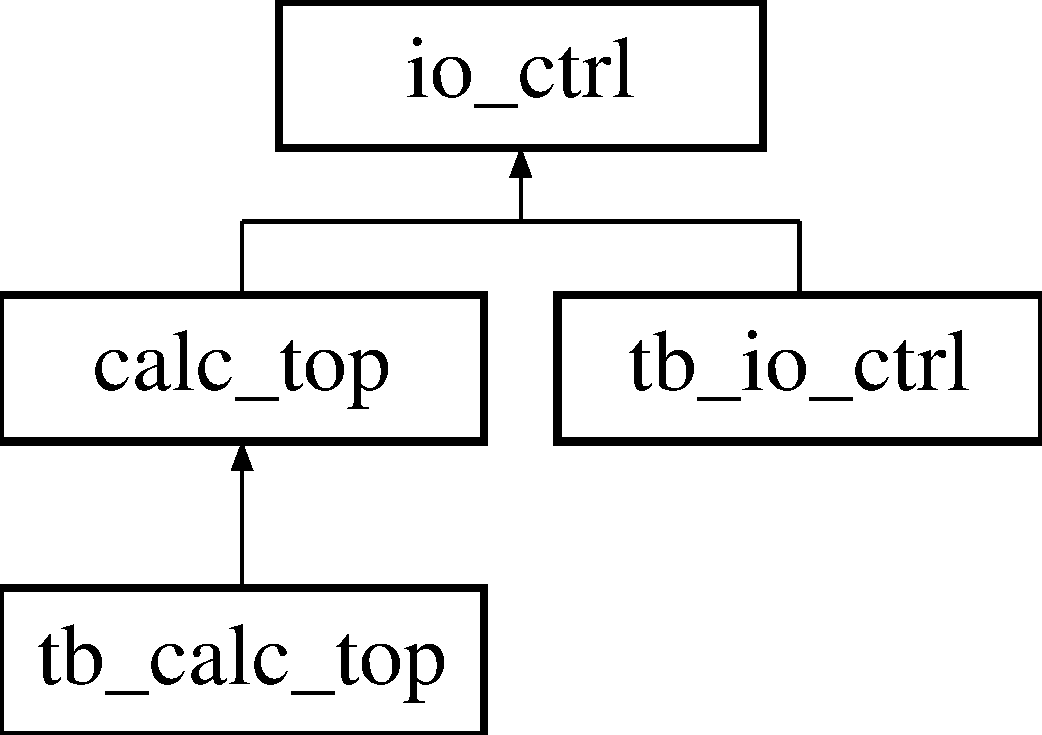
\includegraphics[height=3.000000cm]{classio__ctrl}
\end{center}
\end{figure}
\subsection*{Entities}
\begin{DoxyCompactItemize}
\item 
\hyperlink{classio__ctrl_1_1rtl}{rtl} architecture
\begin{DoxyCompactList}\small\item\em IO Control Unit Architecture R\+TL. \end{DoxyCompactList}\end{DoxyCompactItemize}
\subsection*{Libraries}
 \begin{DoxyCompactItemize}
\item 
\hyperlink{classio__ctrl_ae4f03c286607f3181e16b9aa12d0c6d4}{I\+E\+EE} 
\end{DoxyCompactItemize}
\subsection*{Use Clauses}
 \begin{DoxyCompactItemize}
\item 
\hyperlink{classio__ctrl_acd03516902501cd1c7296a98e22c6fcb}{std\+\_\+logic\+\_\+1164}   
\end{DoxyCompactItemize}
\subsection*{Ports}
 \begin{DoxyCompactItemize}
\item 
\hyperlink{classio__ctrl_abe949478e3f8aad0a6aeb1842fa6c608}{clk\+\_\+i}  {\bfseries {\bfseries \textcolor{keywordflow}{in}\textcolor{vhdlchar}{ }}} {\bfseries \textcolor{comment}{std\+\_\+logic}\textcolor{vhdlchar}{ }} 
\item 
\hyperlink{classio__ctrl_a55da7e76960757f8c6842e86a28ee7be}{reset\+\_\+i}  {\bfseries {\bfseries \textcolor{keywordflow}{in}\textcolor{vhdlchar}{ }}} {\bfseries \textcolor{comment}{std\+\_\+logic}\textcolor{vhdlchar}{ }} 
\item 
\hyperlink{classio__ctrl_a32bd80898d1d7c2a543b82a1d6ad1e6c}{dig0\+\_\+i}  {\bfseries {\bfseries \textcolor{keywordflow}{in}\textcolor{vhdlchar}{ }}} {\bfseries \textcolor{comment}{std\+\_\+logic\+\_\+vector}\textcolor{vhdlchar}{ }\textcolor{vhdlchar}{(}\textcolor{vhdlchar}{ }\textcolor{vhdlchar}{ } \textcolor{vhdldigit}{7} \textcolor{vhdlchar}{ }\textcolor{keywordflow}{downto}\textcolor{vhdlchar}{ }\textcolor{vhdlchar}{ } \textcolor{vhdldigit}{0} \textcolor{vhdlchar}{ }\textcolor{vhdlchar}{)}\textcolor{vhdlchar}{ }} 
\item 
\hyperlink{classio__ctrl_a5038eac0f38fc173af3ff10434e90921}{dig1\+\_\+i}  {\bfseries {\bfseries \textcolor{keywordflow}{in}\textcolor{vhdlchar}{ }}} {\bfseries \textcolor{comment}{std\+\_\+logic\+\_\+vector}\textcolor{vhdlchar}{ }\textcolor{vhdlchar}{(}\textcolor{vhdlchar}{ }\textcolor{vhdlchar}{ } \textcolor{vhdldigit}{7} \textcolor{vhdlchar}{ }\textcolor{keywordflow}{downto}\textcolor{vhdlchar}{ }\textcolor{vhdlchar}{ } \textcolor{vhdldigit}{0} \textcolor{vhdlchar}{ }\textcolor{vhdlchar}{)}\textcolor{vhdlchar}{ }} 
\item 
\hyperlink{classio__ctrl_a1edaf350ab71f6c0e97ba7a82c4bd16f}{dig2\+\_\+i}  {\bfseries {\bfseries \textcolor{keywordflow}{in}\textcolor{vhdlchar}{ }}} {\bfseries \textcolor{comment}{std\+\_\+logic\+\_\+vector}\textcolor{vhdlchar}{ }\textcolor{vhdlchar}{(}\textcolor{vhdlchar}{ }\textcolor{vhdlchar}{ } \textcolor{vhdldigit}{7} \textcolor{vhdlchar}{ }\textcolor{keywordflow}{downto}\textcolor{vhdlchar}{ }\textcolor{vhdlchar}{ } \textcolor{vhdldigit}{0} \textcolor{vhdlchar}{ }\textcolor{vhdlchar}{)}\textcolor{vhdlchar}{ }} 
\item 
\hyperlink{classio__ctrl_ab98d2879f1ba46721cdc9015e3f88d50}{dig3\+\_\+i}  {\bfseries {\bfseries \textcolor{keywordflow}{in}\textcolor{vhdlchar}{ }}} {\bfseries \textcolor{comment}{std\+\_\+logic\+\_\+vector}\textcolor{vhdlchar}{ }\textcolor{vhdlchar}{(}\textcolor{vhdlchar}{ }\textcolor{vhdlchar}{ } \textcolor{vhdldigit}{7} \textcolor{vhdlchar}{ }\textcolor{keywordflow}{downto}\textcolor{vhdlchar}{ }\textcolor{vhdlchar}{ } \textcolor{vhdldigit}{0} \textcolor{vhdlchar}{ }\textcolor{vhdlchar}{)}\textcolor{vhdlchar}{ }} 
\item 
\hyperlink{classio__ctrl_a7693929621a7c94dd62fd7b39db30b50}{led\+\_\+i}  {\bfseries {\bfseries \textcolor{keywordflow}{in}\textcolor{vhdlchar}{ }}} {\bfseries \textcolor{comment}{std\+\_\+logic\+\_\+vector}\textcolor{vhdlchar}{ }\textcolor{vhdlchar}{(}\textcolor{vhdlchar}{ }\textcolor{vhdlchar}{ } \textcolor{vhdldigit}{15} \textcolor{vhdlchar}{ }\textcolor{keywordflow}{downto}\textcolor{vhdlchar}{ }\textcolor{vhdlchar}{ } \textcolor{vhdldigit}{0} \textcolor{vhdlchar}{ }\textcolor{vhdlchar}{)}\textcolor{vhdlchar}{ }} 
\item 
\hyperlink{classio__ctrl_a91628ae1b8a6c62fdd738bc70aba3f1e}{sw\+\_\+i}  {\bfseries {\bfseries \textcolor{keywordflow}{in}\textcolor{vhdlchar}{ }}} {\bfseries \textcolor{comment}{std\+\_\+logic\+\_\+vector}\textcolor{vhdlchar}{ }\textcolor{vhdlchar}{(}\textcolor{vhdlchar}{ }\textcolor{vhdlchar}{ } \textcolor{vhdldigit}{15} \textcolor{vhdlchar}{ }\textcolor{keywordflow}{downto}\textcolor{vhdlchar}{ }\textcolor{vhdlchar}{ } \textcolor{vhdldigit}{0} \textcolor{vhdlchar}{ }\textcolor{vhdlchar}{)}\textcolor{vhdlchar}{ }} 
\item 
\hyperlink{classio__ctrl_ae54d0166fc1acf3023764d9869477e8b}{pb\+\_\+i}  {\bfseries {\bfseries \textcolor{keywordflow}{in}\textcolor{vhdlchar}{ }}} {\bfseries \textcolor{comment}{std\+\_\+logic\+\_\+vector}\textcolor{vhdlchar}{ }\textcolor{vhdlchar}{(}\textcolor{vhdlchar}{ }\textcolor{vhdlchar}{ } \textcolor{vhdldigit}{3} \textcolor{vhdlchar}{ }\textcolor{keywordflow}{downto}\textcolor{vhdlchar}{ }\textcolor{vhdlchar}{ } \textcolor{vhdldigit}{0} \textcolor{vhdlchar}{ }\textcolor{vhdlchar}{)}\textcolor{vhdlchar}{ }} 
\item 
\hyperlink{classio__ctrl_a818bce4de706b73d1b0168e689b5301b}{ss\+\_\+o}  {\bfseries {\bfseries \textcolor{keywordflow}{out}\textcolor{vhdlchar}{ }}} {\bfseries \textcolor{comment}{std\+\_\+logic\+\_\+vector}\textcolor{vhdlchar}{ }\textcolor{vhdlchar}{(}\textcolor{vhdlchar}{ }\textcolor{vhdlchar}{ } \textcolor{vhdldigit}{7} \textcolor{vhdlchar}{ }\textcolor{keywordflow}{downto}\textcolor{vhdlchar}{ }\textcolor{vhdlchar}{ } \textcolor{vhdldigit}{0} \textcolor{vhdlchar}{ }\textcolor{vhdlchar}{)}\textcolor{vhdlchar}{ }} 
\item 
\hyperlink{classio__ctrl_a58671df81269968cc647f9f2335477e9}{ss\+\_\+sel\+\_\+o}  {\bfseries {\bfseries \textcolor{keywordflow}{out}\textcolor{vhdlchar}{ }}} {\bfseries \textcolor{comment}{std\+\_\+logic\+\_\+vector}\textcolor{vhdlchar}{ }\textcolor{vhdlchar}{(}\textcolor{vhdlchar}{ }\textcolor{vhdlchar}{ } \textcolor{vhdldigit}{3} \textcolor{vhdlchar}{ }\textcolor{keywordflow}{downto}\textcolor{vhdlchar}{ }\textcolor{vhdlchar}{ } \textcolor{vhdldigit}{0} \textcolor{vhdlchar}{ }\textcolor{vhdlchar}{)}\textcolor{vhdlchar}{ }} 
\item 
\hyperlink{classio__ctrl_ae622b8b55ca985e4965d79aab895a746}{led\+\_\+o}  {\bfseries {\bfseries \textcolor{keywordflow}{out}\textcolor{vhdlchar}{ }}} {\bfseries \textcolor{comment}{std\+\_\+logic\+\_\+vector}\textcolor{vhdlchar}{ }\textcolor{vhdlchar}{(}\textcolor{vhdlchar}{ }\textcolor{vhdlchar}{ } \textcolor{vhdldigit}{15} \textcolor{vhdlchar}{ }\textcolor{keywordflow}{downto}\textcolor{vhdlchar}{ }\textcolor{vhdlchar}{ } \textcolor{vhdldigit}{0} \textcolor{vhdlchar}{ }\textcolor{vhdlchar}{)}\textcolor{vhdlchar}{ }} 
\item 
\hyperlink{classio__ctrl_a0d67cc1091d658566c78f05fa744f4a0}{swsync\+\_\+o}  {\bfseries {\bfseries \textcolor{keywordflow}{out}\textcolor{vhdlchar}{ }}} {\bfseries \textcolor{comment}{std\+\_\+logic\+\_\+vector}\textcolor{vhdlchar}{ }\textcolor{vhdlchar}{(}\textcolor{vhdlchar}{ }\textcolor{vhdlchar}{ } \textcolor{vhdldigit}{15} \textcolor{vhdlchar}{ }\textcolor{keywordflow}{downto}\textcolor{vhdlchar}{ }\textcolor{vhdlchar}{ } \textcolor{vhdldigit}{0} \textcolor{vhdlchar}{ }\textcolor{vhdlchar}{)}\textcolor{vhdlchar}{ }} 
\item 
\hyperlink{classio__ctrl_a95d4164acb4876609c3ee30095deba32}{pbsync\+\_\+o}  {\bfseries {\bfseries \textcolor{keywordflow}{out}\textcolor{vhdlchar}{ }}} {\bfseries \textcolor{comment}{std\+\_\+logic\+\_\+vector}\textcolor{vhdlchar}{ }\textcolor{vhdlchar}{(}\textcolor{vhdlchar}{ }\textcolor{vhdlchar}{ } \textcolor{vhdldigit}{3} \textcolor{vhdlchar}{ }\textcolor{keywordflow}{downto}\textcolor{vhdlchar}{ }\textcolor{vhdlchar}{ } \textcolor{vhdldigit}{0} \textcolor{vhdlchar}{ }\textcolor{vhdlchar}{)}\textcolor{vhdlchar}{ }} 
\end{DoxyCompactItemize}


\subsection{Detailed Description}
IO Control Unit Entity. 

The IO Control unit is part of the calculator project. 

\subsection{Member Data Documentation}
\mbox{\Hypertarget{classio__ctrl_abe949478e3f8aad0a6aeb1842fa6c608}\label{classio__ctrl_abe949478e3f8aad0a6aeb1842fa6c608}} 
\index{io\+\_\+ctrl@{io\+\_\+ctrl}!clk\+\_\+i@{clk\+\_\+i}}
\index{clk\+\_\+i@{clk\+\_\+i}!io\+\_\+ctrl@{io\+\_\+ctrl}}
\subsubsection{\texorpdfstring{clk\+\_\+i}{clk\_i}}
{\footnotesize\ttfamily \hyperlink{classio__ctrl_abe949478e3f8aad0a6aeb1842fa6c608}{clk\+\_\+i} {\bfseries \textcolor{keywordflow}{in}\textcolor{vhdlchar}{ }} {\bfseries \textcolor{comment}{std\+\_\+logic}\textcolor{vhdlchar}{ }} \hspace{0.3cm}{\ttfamily [Port]}}

\mbox{\Hypertarget{classio__ctrl_a32bd80898d1d7c2a543b82a1d6ad1e6c}\label{classio__ctrl_a32bd80898d1d7c2a543b82a1d6ad1e6c}} 
\index{io\+\_\+ctrl@{io\+\_\+ctrl}!dig0\+\_\+i@{dig0\+\_\+i}}
\index{dig0\+\_\+i@{dig0\+\_\+i}!io\+\_\+ctrl@{io\+\_\+ctrl}}
\subsubsection{\texorpdfstring{dig0\+\_\+i}{dig0\_i}}
{\footnotesize\ttfamily \hyperlink{classio__ctrl_a32bd80898d1d7c2a543b82a1d6ad1e6c}{dig0\+\_\+i} {\bfseries \textcolor{keywordflow}{in}\textcolor{vhdlchar}{ }} {\bfseries \textcolor{comment}{std\+\_\+logic\+\_\+vector}\textcolor{vhdlchar}{ }\textcolor{vhdlchar}{(}\textcolor{vhdlchar}{ }\textcolor{vhdlchar}{ } \textcolor{vhdldigit}{7} \textcolor{vhdlchar}{ }\textcolor{keywordflow}{downto}\textcolor{vhdlchar}{ }\textcolor{vhdlchar}{ } \textcolor{vhdldigit}{0} \textcolor{vhdlchar}{ }\textcolor{vhdlchar}{)}\textcolor{vhdlchar}{ }} \hspace{0.3cm}{\ttfamily [Port]}}

\mbox{\Hypertarget{classio__ctrl_a5038eac0f38fc173af3ff10434e90921}\label{classio__ctrl_a5038eac0f38fc173af3ff10434e90921}} 
\index{io\+\_\+ctrl@{io\+\_\+ctrl}!dig1\+\_\+i@{dig1\+\_\+i}}
\index{dig1\+\_\+i@{dig1\+\_\+i}!io\+\_\+ctrl@{io\+\_\+ctrl}}
\subsubsection{\texorpdfstring{dig1\+\_\+i}{dig1\_i}}
{\footnotesize\ttfamily \hyperlink{classio__ctrl_a5038eac0f38fc173af3ff10434e90921}{dig1\+\_\+i} {\bfseries \textcolor{keywordflow}{in}\textcolor{vhdlchar}{ }} {\bfseries \textcolor{comment}{std\+\_\+logic\+\_\+vector}\textcolor{vhdlchar}{ }\textcolor{vhdlchar}{(}\textcolor{vhdlchar}{ }\textcolor{vhdlchar}{ } \textcolor{vhdldigit}{7} \textcolor{vhdlchar}{ }\textcolor{keywordflow}{downto}\textcolor{vhdlchar}{ }\textcolor{vhdlchar}{ } \textcolor{vhdldigit}{0} \textcolor{vhdlchar}{ }\textcolor{vhdlchar}{)}\textcolor{vhdlchar}{ }} \hspace{0.3cm}{\ttfamily [Port]}}

\mbox{\Hypertarget{classio__ctrl_a1edaf350ab71f6c0e97ba7a82c4bd16f}\label{classio__ctrl_a1edaf350ab71f6c0e97ba7a82c4bd16f}} 
\index{io\+\_\+ctrl@{io\+\_\+ctrl}!dig2\+\_\+i@{dig2\+\_\+i}}
\index{dig2\+\_\+i@{dig2\+\_\+i}!io\+\_\+ctrl@{io\+\_\+ctrl}}
\subsubsection{\texorpdfstring{dig2\+\_\+i}{dig2\_i}}
{\footnotesize\ttfamily \hyperlink{classio__ctrl_a1edaf350ab71f6c0e97ba7a82c4bd16f}{dig2\+\_\+i} {\bfseries \textcolor{keywordflow}{in}\textcolor{vhdlchar}{ }} {\bfseries \textcolor{comment}{std\+\_\+logic\+\_\+vector}\textcolor{vhdlchar}{ }\textcolor{vhdlchar}{(}\textcolor{vhdlchar}{ }\textcolor{vhdlchar}{ } \textcolor{vhdldigit}{7} \textcolor{vhdlchar}{ }\textcolor{keywordflow}{downto}\textcolor{vhdlchar}{ }\textcolor{vhdlchar}{ } \textcolor{vhdldigit}{0} \textcolor{vhdlchar}{ }\textcolor{vhdlchar}{)}\textcolor{vhdlchar}{ }} \hspace{0.3cm}{\ttfamily [Port]}}

\mbox{\Hypertarget{classio__ctrl_ab98d2879f1ba46721cdc9015e3f88d50}\label{classio__ctrl_ab98d2879f1ba46721cdc9015e3f88d50}} 
\index{io\+\_\+ctrl@{io\+\_\+ctrl}!dig3\+\_\+i@{dig3\+\_\+i}}
\index{dig3\+\_\+i@{dig3\+\_\+i}!io\+\_\+ctrl@{io\+\_\+ctrl}}
\subsubsection{\texorpdfstring{dig3\+\_\+i}{dig3\_i}}
{\footnotesize\ttfamily \hyperlink{classio__ctrl_ab98d2879f1ba46721cdc9015e3f88d50}{dig3\+\_\+i} {\bfseries \textcolor{keywordflow}{in}\textcolor{vhdlchar}{ }} {\bfseries \textcolor{comment}{std\+\_\+logic\+\_\+vector}\textcolor{vhdlchar}{ }\textcolor{vhdlchar}{(}\textcolor{vhdlchar}{ }\textcolor{vhdlchar}{ } \textcolor{vhdldigit}{7} \textcolor{vhdlchar}{ }\textcolor{keywordflow}{downto}\textcolor{vhdlchar}{ }\textcolor{vhdlchar}{ } \textcolor{vhdldigit}{0} \textcolor{vhdlchar}{ }\textcolor{vhdlchar}{)}\textcolor{vhdlchar}{ }} \hspace{0.3cm}{\ttfamily [Port]}}

\mbox{\Hypertarget{classio__ctrl_ae4f03c286607f3181e16b9aa12d0c6d4}\label{classio__ctrl_ae4f03c286607f3181e16b9aa12d0c6d4}} 
\index{io\+\_\+ctrl@{io\+\_\+ctrl}!I\+E\+EE@{I\+E\+EE}}
\index{I\+E\+EE@{I\+E\+EE}!io\+\_\+ctrl@{io\+\_\+ctrl}}
\subsubsection{\texorpdfstring{I\+E\+EE}{IEEE}}
{\footnotesize\ttfamily \hyperlink{classio__ctrl_ae4f03c286607f3181e16b9aa12d0c6d4}{I\+E\+EE}\hspace{0.3cm}{\ttfamily [Library]}}

\mbox{\Hypertarget{classio__ctrl_a7693929621a7c94dd62fd7b39db30b50}\label{classio__ctrl_a7693929621a7c94dd62fd7b39db30b50}} 
\index{io\+\_\+ctrl@{io\+\_\+ctrl}!led\+\_\+i@{led\+\_\+i}}
\index{led\+\_\+i@{led\+\_\+i}!io\+\_\+ctrl@{io\+\_\+ctrl}}
\subsubsection{\texorpdfstring{led\+\_\+i}{led\_i}}
{\footnotesize\ttfamily \hyperlink{classio__ctrl_a7693929621a7c94dd62fd7b39db30b50}{led\+\_\+i} {\bfseries \textcolor{keywordflow}{in}\textcolor{vhdlchar}{ }} {\bfseries \textcolor{comment}{std\+\_\+logic\+\_\+vector}\textcolor{vhdlchar}{ }\textcolor{vhdlchar}{(}\textcolor{vhdlchar}{ }\textcolor{vhdlchar}{ } \textcolor{vhdldigit}{15} \textcolor{vhdlchar}{ }\textcolor{keywordflow}{downto}\textcolor{vhdlchar}{ }\textcolor{vhdlchar}{ } \textcolor{vhdldigit}{0} \textcolor{vhdlchar}{ }\textcolor{vhdlchar}{)}\textcolor{vhdlchar}{ }} \hspace{0.3cm}{\ttfamily [Port]}}

\mbox{\Hypertarget{classio__ctrl_ae622b8b55ca985e4965d79aab895a746}\label{classio__ctrl_ae622b8b55ca985e4965d79aab895a746}} 
\index{io\+\_\+ctrl@{io\+\_\+ctrl}!led\+\_\+o@{led\+\_\+o}}
\index{led\+\_\+o@{led\+\_\+o}!io\+\_\+ctrl@{io\+\_\+ctrl}}
\subsubsection{\texorpdfstring{led\+\_\+o}{led\_o}}
{\footnotesize\ttfamily \hyperlink{classio__ctrl_ae622b8b55ca985e4965d79aab895a746}{led\+\_\+o} {\bfseries \textcolor{keywordflow}{out}\textcolor{vhdlchar}{ }} {\bfseries \textcolor{comment}{std\+\_\+logic\+\_\+vector}\textcolor{vhdlchar}{ }\textcolor{vhdlchar}{(}\textcolor{vhdlchar}{ }\textcolor{vhdlchar}{ } \textcolor{vhdldigit}{15} \textcolor{vhdlchar}{ }\textcolor{keywordflow}{downto}\textcolor{vhdlchar}{ }\textcolor{vhdlchar}{ } \textcolor{vhdldigit}{0} \textcolor{vhdlchar}{ }\textcolor{vhdlchar}{)}\textcolor{vhdlchar}{ }} \hspace{0.3cm}{\ttfamily [Port]}}

\mbox{\Hypertarget{classio__ctrl_ae54d0166fc1acf3023764d9869477e8b}\label{classio__ctrl_ae54d0166fc1acf3023764d9869477e8b}} 
\index{io\+\_\+ctrl@{io\+\_\+ctrl}!pb\+\_\+i@{pb\+\_\+i}}
\index{pb\+\_\+i@{pb\+\_\+i}!io\+\_\+ctrl@{io\+\_\+ctrl}}
\subsubsection{\texorpdfstring{pb\+\_\+i}{pb\_i}}
{\footnotesize\ttfamily \hyperlink{classio__ctrl_ae54d0166fc1acf3023764d9869477e8b}{pb\+\_\+i} {\bfseries \textcolor{keywordflow}{in}\textcolor{vhdlchar}{ }} {\bfseries \textcolor{comment}{std\+\_\+logic\+\_\+vector}\textcolor{vhdlchar}{ }\textcolor{vhdlchar}{(}\textcolor{vhdlchar}{ }\textcolor{vhdlchar}{ } \textcolor{vhdldigit}{3} \textcolor{vhdlchar}{ }\textcolor{keywordflow}{downto}\textcolor{vhdlchar}{ }\textcolor{vhdlchar}{ } \textcolor{vhdldigit}{0} \textcolor{vhdlchar}{ }\textcolor{vhdlchar}{)}\textcolor{vhdlchar}{ }} \hspace{0.3cm}{\ttfamily [Port]}}

\mbox{\Hypertarget{classio__ctrl_a95d4164acb4876609c3ee30095deba32}\label{classio__ctrl_a95d4164acb4876609c3ee30095deba32}} 
\index{io\+\_\+ctrl@{io\+\_\+ctrl}!pbsync\+\_\+o@{pbsync\+\_\+o}}
\index{pbsync\+\_\+o@{pbsync\+\_\+o}!io\+\_\+ctrl@{io\+\_\+ctrl}}
\subsubsection{\texorpdfstring{pbsync\+\_\+o}{pbsync\_o}}
{\footnotesize\ttfamily \hyperlink{classio__ctrl_a95d4164acb4876609c3ee30095deba32}{pbsync\+\_\+o} {\bfseries \textcolor{keywordflow}{out}\textcolor{vhdlchar}{ }} {\bfseries \textcolor{comment}{std\+\_\+logic\+\_\+vector}\textcolor{vhdlchar}{ }\textcolor{vhdlchar}{(}\textcolor{vhdlchar}{ }\textcolor{vhdlchar}{ } \textcolor{vhdldigit}{3} \textcolor{vhdlchar}{ }\textcolor{keywordflow}{downto}\textcolor{vhdlchar}{ }\textcolor{vhdlchar}{ } \textcolor{vhdldigit}{0} \textcolor{vhdlchar}{ }\textcolor{vhdlchar}{)}\textcolor{vhdlchar}{ }} \hspace{0.3cm}{\ttfamily [Port]}}

\mbox{\Hypertarget{classio__ctrl_a55da7e76960757f8c6842e86a28ee7be}\label{classio__ctrl_a55da7e76960757f8c6842e86a28ee7be}} 
\index{io\+\_\+ctrl@{io\+\_\+ctrl}!reset\+\_\+i@{reset\+\_\+i}}
\index{reset\+\_\+i@{reset\+\_\+i}!io\+\_\+ctrl@{io\+\_\+ctrl}}
\subsubsection{\texorpdfstring{reset\+\_\+i}{reset\_i}}
{\footnotesize\ttfamily \hyperlink{classio__ctrl_a55da7e76960757f8c6842e86a28ee7be}{reset\+\_\+i} {\bfseries \textcolor{keywordflow}{in}\textcolor{vhdlchar}{ }} {\bfseries \textcolor{comment}{std\+\_\+logic}\textcolor{vhdlchar}{ }} \hspace{0.3cm}{\ttfamily [Port]}}

\mbox{\Hypertarget{classio__ctrl_a818bce4de706b73d1b0168e689b5301b}\label{classio__ctrl_a818bce4de706b73d1b0168e689b5301b}} 
\index{io\+\_\+ctrl@{io\+\_\+ctrl}!ss\+\_\+o@{ss\+\_\+o}}
\index{ss\+\_\+o@{ss\+\_\+o}!io\+\_\+ctrl@{io\+\_\+ctrl}}
\subsubsection{\texorpdfstring{ss\+\_\+o}{ss\_o}}
{\footnotesize\ttfamily \hyperlink{classio__ctrl_a818bce4de706b73d1b0168e689b5301b}{ss\+\_\+o} {\bfseries \textcolor{keywordflow}{out}\textcolor{vhdlchar}{ }} {\bfseries \textcolor{comment}{std\+\_\+logic\+\_\+vector}\textcolor{vhdlchar}{ }\textcolor{vhdlchar}{(}\textcolor{vhdlchar}{ }\textcolor{vhdlchar}{ } \textcolor{vhdldigit}{7} \textcolor{vhdlchar}{ }\textcolor{keywordflow}{downto}\textcolor{vhdlchar}{ }\textcolor{vhdlchar}{ } \textcolor{vhdldigit}{0} \textcolor{vhdlchar}{ }\textcolor{vhdlchar}{)}\textcolor{vhdlchar}{ }} \hspace{0.3cm}{\ttfamily [Port]}}

\mbox{\Hypertarget{classio__ctrl_a58671df81269968cc647f9f2335477e9}\label{classio__ctrl_a58671df81269968cc647f9f2335477e9}} 
\index{io\+\_\+ctrl@{io\+\_\+ctrl}!ss\+\_\+sel\+\_\+o@{ss\+\_\+sel\+\_\+o}}
\index{ss\+\_\+sel\+\_\+o@{ss\+\_\+sel\+\_\+o}!io\+\_\+ctrl@{io\+\_\+ctrl}}
\subsubsection{\texorpdfstring{ss\+\_\+sel\+\_\+o}{ss\_sel\_o}}
{\footnotesize\ttfamily \hyperlink{classio__ctrl_a58671df81269968cc647f9f2335477e9}{ss\+\_\+sel\+\_\+o} {\bfseries \textcolor{keywordflow}{out}\textcolor{vhdlchar}{ }} {\bfseries \textcolor{comment}{std\+\_\+logic\+\_\+vector}\textcolor{vhdlchar}{ }\textcolor{vhdlchar}{(}\textcolor{vhdlchar}{ }\textcolor{vhdlchar}{ } \textcolor{vhdldigit}{3} \textcolor{vhdlchar}{ }\textcolor{keywordflow}{downto}\textcolor{vhdlchar}{ }\textcolor{vhdlchar}{ } \textcolor{vhdldigit}{0} \textcolor{vhdlchar}{ }\textcolor{vhdlchar}{)}\textcolor{vhdlchar}{ }} \hspace{0.3cm}{\ttfamily [Port]}}

\mbox{\Hypertarget{classio__ctrl_acd03516902501cd1c7296a98e22c6fcb}\label{classio__ctrl_acd03516902501cd1c7296a98e22c6fcb}} 
\index{io\+\_\+ctrl@{io\+\_\+ctrl}!std\+\_\+logic\+\_\+1164@{std\+\_\+logic\+\_\+1164}}
\index{std\+\_\+logic\+\_\+1164@{std\+\_\+logic\+\_\+1164}!io\+\_\+ctrl@{io\+\_\+ctrl}}
\subsubsection{\texorpdfstring{std\+\_\+logic\+\_\+1164}{std\_logic\_1164}}
{\footnotesize\ttfamily \hyperlink{classio__ctrl_acd03516902501cd1c7296a98e22c6fcb}{std\+\_\+logic\+\_\+1164}\hspace{0.3cm}{\ttfamily [Package]}}

\mbox{\Hypertarget{classio__ctrl_a91628ae1b8a6c62fdd738bc70aba3f1e}\label{classio__ctrl_a91628ae1b8a6c62fdd738bc70aba3f1e}} 
\index{io\+\_\+ctrl@{io\+\_\+ctrl}!sw\+\_\+i@{sw\+\_\+i}}
\index{sw\+\_\+i@{sw\+\_\+i}!io\+\_\+ctrl@{io\+\_\+ctrl}}
\subsubsection{\texorpdfstring{sw\+\_\+i}{sw\_i}}
{\footnotesize\ttfamily \hyperlink{classio__ctrl_a91628ae1b8a6c62fdd738bc70aba3f1e}{sw\+\_\+i} {\bfseries \textcolor{keywordflow}{in}\textcolor{vhdlchar}{ }} {\bfseries \textcolor{comment}{std\+\_\+logic\+\_\+vector}\textcolor{vhdlchar}{ }\textcolor{vhdlchar}{(}\textcolor{vhdlchar}{ }\textcolor{vhdlchar}{ } \textcolor{vhdldigit}{15} \textcolor{vhdlchar}{ }\textcolor{keywordflow}{downto}\textcolor{vhdlchar}{ }\textcolor{vhdlchar}{ } \textcolor{vhdldigit}{0} \textcolor{vhdlchar}{ }\textcolor{vhdlchar}{)}\textcolor{vhdlchar}{ }} \hspace{0.3cm}{\ttfamily [Port]}}

\mbox{\Hypertarget{classio__ctrl_a0d67cc1091d658566c78f05fa744f4a0}\label{classio__ctrl_a0d67cc1091d658566c78f05fa744f4a0}} 
\index{io\+\_\+ctrl@{io\+\_\+ctrl}!swsync\+\_\+o@{swsync\+\_\+o}}
\index{swsync\+\_\+o@{swsync\+\_\+o}!io\+\_\+ctrl@{io\+\_\+ctrl}}
\subsubsection{\texorpdfstring{swsync\+\_\+o}{swsync\_o}}
{\footnotesize\ttfamily \hyperlink{classio__ctrl_a0d67cc1091d658566c78f05fa744f4a0}{swsync\+\_\+o} {\bfseries \textcolor{keywordflow}{out}\textcolor{vhdlchar}{ }} {\bfseries \textcolor{comment}{std\+\_\+logic\+\_\+vector}\textcolor{vhdlchar}{ }\textcolor{vhdlchar}{(}\textcolor{vhdlchar}{ }\textcolor{vhdlchar}{ } \textcolor{vhdldigit}{15} \textcolor{vhdlchar}{ }\textcolor{keywordflow}{downto}\textcolor{vhdlchar}{ }\textcolor{vhdlchar}{ } \textcolor{vhdldigit}{0} \textcolor{vhdlchar}{ }\textcolor{vhdlchar}{)}\textcolor{vhdlchar}{ }} \hspace{0.3cm}{\ttfamily [Port]}}



The documentation for this class was generated from the following file\+:\begin{DoxyCompactItemize}
\item 
vhdl/\hyperlink{io__ctrl___8vhd}{io\+\_\+ctrl\+\_\+.\+vhd}\end{DoxyCompactItemize}

\hypertarget{classio__ctrl_1_1rtl}{}\section{rtl Architecture Reference}
\label{classio__ctrl_1_1rtl}\index{rtl@{rtl}}


IO Control Unit Architecture.  


\subsection*{Processes}
 \begin{DoxyCompactItemize}
\item 
\hyperlink{classio__ctrl_1_1rtl_ae82c89fe12aec7f3a8a04e832dd5cc0e}{p\+\_\+slowen}{\bfseries  ( {\bfseries \textcolor{vhdlchar}{clk\+\_\+i}\textcolor{vhdlchar}{ }} , {\bfseries \textcolor{vhdlchar}{reset\+\_\+i}\textcolor{vhdlchar}{ }} )}
\begin{DoxyCompactList}\small\item\em IO Control Unit Architecture. \end{DoxyCompactList}\item 
\hyperlink{classio__ctrl_1_1rtl_a627aed9352c04ffc84d1b682c4da9ba5}{p\+\_\+debounce}{\bfseries  ( {\bfseries \textcolor{vhdlchar}{clk\+\_\+i}\textcolor{vhdlchar}{ }} , {\bfseries \textcolor{vhdlchar}{reset\+\_\+i}\textcolor{vhdlchar}{ }} )}
\begin{DoxyCompactList}\small\item\em IO Control Unit Architecture. \end{DoxyCompactList}\item 
\hyperlink{classio__ctrl_1_1rtl_a9adae6696d8563868e95204ecd77e739}{p\+\_\+display\+\_\+ctrl}{\bfseries  ( {\bfseries \textcolor{vhdlchar}{clk\+\_\+i}\textcolor{vhdlchar}{ }} , {\bfseries \textcolor{vhdlchar}{reset\+\_\+i}\textcolor{vhdlchar}{ }} )}
\begin{DoxyCompactList}\small\item\em IO Control Unit Architecture. \end{DoxyCompactList}\end{DoxyCompactItemize}
\subsection*{Libraries}
 \begin{DoxyCompactItemize}
\item 
\mbox{\Hypertarget{classio__ctrl_1_1rtl_ae4f03c286607f3181e16b9aa12d0c6d4}\label{classio__ctrl_1_1rtl_ae4f03c286607f3181e16b9aa12d0c6d4}} 
\hyperlink{classio__ctrl_1_1rtl_ae4f03c286607f3181e16b9aa12d0c6d4}{I\+E\+EE} 
\end{DoxyCompactItemize}
\subsection*{Use Clauses}
 \begin{DoxyCompactItemize}
\item 
\mbox{\Hypertarget{classio__ctrl_1_1rtl_acd03516902501cd1c7296a98e22c6fcb}\label{classio__ctrl_1_1rtl_acd03516902501cd1c7296a98e22c6fcb}} 
\hyperlink{classio__ctrl_1_1rtl_acd03516902501cd1c7296a98e22c6fcb}{std\+\_\+logic\+\_\+1164}   
\item 
\mbox{\Hypertarget{classio__ctrl_1_1rtl_a0f5ecc6613f63d07f7963a97b1b26095}\label{classio__ctrl_1_1rtl_a0f5ecc6613f63d07f7963a97b1b26095}} 
\hyperlink{classio__ctrl_1_1rtl_a0f5ecc6613f63d07f7963a97b1b26095}{std\+\_\+logic\+\_\+arith}   
\end{DoxyCompactItemize}
\subsection*{Constants}
 \begin{DoxyCompactItemize}
\item 
\mbox{\Hypertarget{classio__ctrl_1_1rtl_a85d68696ce8aad74f4f3f0f5d6cb860a}\label{classio__ctrl_1_1rtl_a85d68696ce8aad74f4f3f0f5d6cb860a}} 
\hyperlink{classio__ctrl_1_1rtl_a85d68696ce8aad74f4f3f0f5d6cb860a}{C\+\_\+\+E\+N\+C\+O\+U\+N\+T\+V\+AL} {\bfseries \textcolor{vhdlchar}{std\+\_\+logic\+\_\+vector}\textcolor{vhdlchar}{ }\textcolor{vhdlchar}{(}\textcolor{vhdlchar}{ }\textcolor{vhdlchar}{ } \textcolor{vhdldigit}{16} \textcolor{vhdlchar}{ }\textcolor{vhdlchar}{downto}\textcolor{vhdlchar}{ }\textcolor{vhdlchar}{ } \textcolor{vhdldigit}{0} \textcolor{vhdlchar}{ }\textcolor{vhdlchar}{)}\textcolor{vhdlchar}{ }\textcolor{vhdlchar}{ }\textcolor{vhdlchar}{ }\textcolor{vhdlchar}{\+:}\textcolor{vhdlchar}{=}\textcolor{vhdlchar}{ }\textcolor{vhdlchar}{ }\textcolor{vhdlchar}{ }\textcolor{vhdlchar}{ }\textcolor{keyword}{\char`\"{} 11000011010100000 \char`\"{}}\textcolor{vhdlchar}{ }} 
\end{DoxyCompactItemize}
\subsection*{Signals}
 \begin{DoxyCompactItemize}
\item 
\mbox{\Hypertarget{classio__ctrl_1_1rtl_a3280fe5d78cf2b9c6e3160d7855f3168}\label{classio__ctrl_1_1rtl_a3280fe5d78cf2b9c6e3160d7855f3168}} 
\hyperlink{classio__ctrl_1_1rtl_a3280fe5d78cf2b9c6e3160d7855f3168}{s\+\_\+enctr} {\bfseries \textcolor{vhdlchar}{std\+\_\+logic\+\_\+vector}\textcolor{vhdlchar}{ }\textcolor{vhdlchar}{(}\textcolor{vhdlchar}{ }\textcolor{vhdlchar}{ } \textcolor{vhdldigit}{16} \textcolor{vhdlchar}{ }\textcolor{vhdlchar}{downto}\textcolor{vhdlchar}{ }\textcolor{vhdlchar}{ } \textcolor{vhdldigit}{0} \textcolor{vhdlchar}{ }\textcolor{vhdlchar}{)}\textcolor{vhdlchar}{ }} 
\item 
\mbox{\Hypertarget{classio__ctrl_1_1rtl_a6f6967086ba7f5aa15cf15dc1017e1ee}\label{classio__ctrl_1_1rtl_a6f6967086ba7f5aa15cf15dc1017e1ee}} 
\hyperlink{classio__ctrl_1_1rtl_a6f6967086ba7f5aa15cf15dc1017e1ee}{s\+\_\+1khzen} {\bfseries \textcolor{vhdlchar}{std\+\_\+logic}\textcolor{vhdlchar}{ }} 
\item 
\mbox{\Hypertarget{classio__ctrl_1_1rtl_a9beb24b7dc36ee4c13f031555d2ceb3c}\label{classio__ctrl_1_1rtl_a9beb24b7dc36ee4c13f031555d2ceb3c}} 
\hyperlink{classio__ctrl_1_1rtl_a9beb24b7dc36ee4c13f031555d2ceb3c}{swsync} {\bfseries \textcolor{vhdlchar}{std\+\_\+logic\+\_\+vector}\textcolor{vhdlchar}{ }\textcolor{vhdlchar}{(}\textcolor{vhdlchar}{ }\textcolor{vhdlchar}{ } \textcolor{vhdldigit}{15} \textcolor{vhdlchar}{ }\textcolor{vhdlchar}{downto}\textcolor{vhdlchar}{ }\textcolor{vhdlchar}{ } \textcolor{vhdldigit}{0} \textcolor{vhdlchar}{ }\textcolor{vhdlchar}{)}\textcolor{vhdlchar}{ }} 
\item 
\mbox{\Hypertarget{classio__ctrl_1_1rtl_a5c1bd4d44af9b0f340317c2228eda942}\label{classio__ctrl_1_1rtl_a5c1bd4d44af9b0f340317c2228eda942}} 
\hyperlink{classio__ctrl_1_1rtl_a5c1bd4d44af9b0f340317c2228eda942}{pbsync} {\bfseries \textcolor{vhdlchar}{std\+\_\+logic\+\_\+vector}\textcolor{vhdlchar}{ }\textcolor{vhdlchar}{(}\textcolor{vhdlchar}{ }\textcolor{vhdlchar}{ } \textcolor{vhdldigit}{3} \textcolor{vhdlchar}{ }\textcolor{vhdlchar}{downto}\textcolor{vhdlchar}{ }\textcolor{vhdlchar}{ } \textcolor{vhdldigit}{0} \textcolor{vhdlchar}{ }\textcolor{vhdlchar}{)}\textcolor{vhdlchar}{ }} 
\item 
\mbox{\Hypertarget{classio__ctrl_1_1rtl_a004d6c8caba65b687289b36ecea87a98}\label{classio__ctrl_1_1rtl_a004d6c8caba65b687289b36ecea87a98}} 
\hyperlink{classio__ctrl_1_1rtl_a004d6c8caba65b687289b36ecea87a98}{s\+\_\+ss\+\_\+sel} {\bfseries \textcolor{vhdlchar}{std\+\_\+logic\+\_\+vector}\textcolor{vhdlchar}{ }\textcolor{vhdlchar}{(}\textcolor{vhdlchar}{ }\textcolor{vhdlchar}{ } \textcolor{vhdldigit}{3} \textcolor{vhdlchar}{ }\textcolor{vhdlchar}{downto}\textcolor{vhdlchar}{ }\textcolor{vhdlchar}{ } \textcolor{vhdldigit}{0} \textcolor{vhdlchar}{ }\textcolor{vhdlchar}{)}\textcolor{vhdlchar}{ }} 
\item 
\mbox{\Hypertarget{classio__ctrl_1_1rtl_ad246180727a4d128207d3681d61db04d}\label{classio__ctrl_1_1rtl_ad246180727a4d128207d3681d61db04d}} 
\hyperlink{classio__ctrl_1_1rtl_ad246180727a4d128207d3681d61db04d}{s\+\_\+ss} {\bfseries \textcolor{vhdlchar}{std\+\_\+logic\+\_\+vector}\textcolor{vhdlchar}{ }\textcolor{vhdlchar}{(}\textcolor{vhdlchar}{ }\textcolor{vhdlchar}{ } \textcolor{vhdldigit}{7} \textcolor{vhdlchar}{ }\textcolor{vhdlchar}{downto}\textcolor{vhdlchar}{ }\textcolor{vhdlchar}{ } \textcolor{vhdldigit}{0} \textcolor{vhdlchar}{ }\textcolor{vhdlchar}{)}\textcolor{vhdlchar}{ }} 
\item 
\mbox{\Hypertarget{classio__ctrl_1_1rtl_a8ccbdb26e3f7c6ca59e3b30524abd69a}\label{classio__ctrl_1_1rtl_a8ccbdb26e3f7c6ca59e3b30524abd69a}} 
\hyperlink{classio__ctrl_1_1rtl_a8ccbdb26e3f7c6ca59e3b30524abd69a}{s\+\_\+muxcnt} {\bfseries \textcolor{vhdlchar}{std\+\_\+logic\+\_\+vector}\textcolor{vhdlchar}{ }\textcolor{vhdlchar}{(}\textcolor{vhdlchar}{ }\textcolor{vhdlchar}{ } \textcolor{vhdldigit}{1} \textcolor{vhdlchar}{ }\textcolor{vhdlchar}{downto}\textcolor{vhdlchar}{ }\textcolor{vhdlchar}{ } \textcolor{vhdldigit}{0} \textcolor{vhdlchar}{ }\textcolor{vhdlchar}{)}\textcolor{vhdlchar}{ }} 
\item 
\mbox{\Hypertarget{classio__ctrl_1_1rtl_a6f1a8f78ddc25f65e38808e8a815afdd}\label{classio__ctrl_1_1rtl_a6f1a8f78ddc25f65e38808e8a815afdd}} 
\hyperlink{classio__ctrl_1_1rtl_a6f1a8f78ddc25f65e38808e8a815afdd}{s\+\_\+debcnt} {\bfseries \textcolor{vhdlchar}{std\+\_\+logic\+\_\+vector}\textcolor{vhdlchar}{ }\textcolor{vhdlchar}{(}\textcolor{vhdlchar}{ }\textcolor{vhdlchar}{ } \textcolor{vhdldigit}{3} \textcolor{vhdlchar}{ }\textcolor{vhdlchar}{downto}\textcolor{vhdlchar}{ }\textcolor{vhdlchar}{ } \textcolor{vhdldigit}{0} \textcolor{vhdlchar}{ }\textcolor{vhdlchar}{)}\textcolor{vhdlchar}{ }} 
\end{DoxyCompactItemize}


\subsection{Detailed Description}
IO Control Unit Architecture. 

The IO Control uniti part of the calculator project. 

\subsection{Member Function Documentation}
\mbox{\Hypertarget{classio__ctrl_1_1rtl_a627aed9352c04ffc84d1b682c4da9ba5}\label{classio__ctrl_1_1rtl_a627aed9352c04ffc84d1b682c4da9ba5}} 
\index{io\+\_\+ctrl\+::rtl@{io\+\_\+ctrl\+::rtl}!p\+\_\+debounce@{p\+\_\+debounce}}
\index{p\+\_\+debounce@{p\+\_\+debounce}!io\+\_\+ctrl\+::rtl@{io\+\_\+ctrl\+::rtl}}
\subsubsection{\texorpdfstring{p\+\_\+debounce()}{p\_debounce()}}
{\footnotesize\ttfamily  {\bfseries \textcolor{vhdlchar}{ }} p\+\_\+debounce(\begin{DoxyParamCaption}\item[{}]{{\bfseries \textcolor{vhdlchar}{clk\+\_\+i}\textcolor{vhdlchar}{ }} {\em } ,  }\item[{}]{{\bfseries \textcolor{vhdlchar}{reset\+\_\+i}\textcolor{vhdlchar}{ }} {\em } }\end{DoxyParamCaption})\hspace{0.3cm}{\ttfamily [Process]}}



IO Control Unit Architecture. 

Process for button debounce. \mbox{\Hypertarget{classio__ctrl_1_1rtl_a9adae6696d8563868e95204ecd77e739}\label{classio__ctrl_1_1rtl_a9adae6696d8563868e95204ecd77e739}} 
\index{io\+\_\+ctrl\+::rtl@{io\+\_\+ctrl\+::rtl}!p\+\_\+display\+\_\+ctrl@{p\+\_\+display\+\_\+ctrl}}
\index{p\+\_\+display\+\_\+ctrl@{p\+\_\+display\+\_\+ctrl}!io\+\_\+ctrl\+::rtl@{io\+\_\+ctrl\+::rtl}}
\subsubsection{\texorpdfstring{p\+\_\+display\+\_\+ctrl()}{p\_display\_ctrl()}}
{\footnotesize\ttfamily  {\bfseries \textcolor{vhdlchar}{ }} p\+\_\+display\+\_\+ctrl(\begin{DoxyParamCaption}\item[{}]{{\bfseries \textcolor{vhdlchar}{clk\+\_\+i}\textcolor{vhdlchar}{ }} {\em } ,  }\item[{}]{{\bfseries \textcolor{vhdlchar}{reset\+\_\+i}\textcolor{vhdlchar}{ }} {\em } }\end{DoxyParamCaption})\hspace{0.3cm}{\ttfamily [Process]}}



IO Control Unit Architecture. 

Process to control 7 segment displays. \mbox{\Hypertarget{classio__ctrl_1_1rtl_ae82c89fe12aec7f3a8a04e832dd5cc0e}\label{classio__ctrl_1_1rtl_ae82c89fe12aec7f3a8a04e832dd5cc0e}} 
\index{io\+\_\+ctrl\+::rtl@{io\+\_\+ctrl\+::rtl}!p\+\_\+slowen@{p\+\_\+slowen}}
\index{p\+\_\+slowen@{p\+\_\+slowen}!io\+\_\+ctrl\+::rtl@{io\+\_\+ctrl\+::rtl}}
\subsubsection{\texorpdfstring{p\+\_\+slowen()}{p\_slowen()}}
{\footnotesize\ttfamily  {\bfseries \textcolor{vhdlchar}{ }} p\+\_\+slowen(\begin{DoxyParamCaption}\item[{}]{{\bfseries \textcolor{vhdlchar}{clk\+\_\+i}\textcolor{vhdlchar}{ }} {\em } ,  }\item[{}]{{\bfseries \textcolor{vhdlchar}{reset\+\_\+i}\textcolor{vhdlchar}{ }} {\em } }\end{DoxyParamCaption})\hspace{0.3cm}{\ttfamily [Process]}}



IO Control Unit Architecture. 

Process for 1k\+Hz signal. 

The documentation for this class was generated from the following file\+:\begin{DoxyCompactItemize}
\item 
vhdl/\hyperlink{io__ctrl__rtl_8vhd}{io\+\_\+ctrl\+\_\+rtl.\+vhd}\end{DoxyCompactItemize}

\hypertarget{classalu_1_1rtl}{}\section{rtl Architecture Reference}
\label{classalu_1_1rtl}\index{rtl@{rtl}}


A\+LU Architecture R\+TL.  


\subsection*{Processes}
 \begin{DoxyCompactItemize}
\item 
\hyperlink{classalu_1_1rtl_a127a47776b4d018774cd0c1842fb6038}{calculate}{\bfseries  ( {\bfseries {\bfseries \hyperlink{classalu_abe949478e3f8aad0a6aeb1842fa6c608}{clk\+\_\+i}} \textcolor{vhdlchar}{ }} , {\bfseries {\bfseries \hyperlink{classalu_a55da7e76960757f8c6842e86a28ee7be}{reset\+\_\+i}} \textcolor{vhdlchar}{ }} , {\bfseries {\bfseries \hyperlink{classalu_aba7911228d421cdfd5fc4eb74a60572c}{start\+\_\+i}} \textcolor{vhdlchar}{ }} , {\bfseries {\bfseries \hyperlink{classalu_1_1rtl_abb13f4e66b38434991c4a6e11a842d8e}{finished\+\_\+s}} \textcolor{vhdlchar}{ }} , {\bfseries {\bfseries \hyperlink{classalu_1_1rtl_af4334e2915fc133abca5cbbac4312fcf}{run\+\_\+s}} \textcolor{vhdlchar}{ }} , {\bfseries {\bfseries \hyperlink{classalu_a1127482098676cfc6ce7e98ba675ee27}{op1\+\_\+i}} \textcolor{vhdlchar}{ }} , {\bfseries {\bfseries \hyperlink{classalu_ae346648ed4ed2217b5e8d668b165aff2}{op2\+\_\+i}} \textcolor{vhdlchar}{ }} , {\bfseries {\bfseries \hyperlink{classalu_aee662ea38c86cd2e7dc1970ce8a6d5e9}{optype\+\_\+i}} \textcolor{vhdlchar}{ }} )}
\begin{DoxyCompactList}\small\item\em A\+LU Architecture R\+TL. \end{DoxyCompactList}\end{DoxyCompactItemize}
\subsection*{Libraries}
 \begin{DoxyCompactItemize}
\item 
\hyperlink{classalu_1_1rtl_ae4f03c286607f3181e16b9aa12d0c6d4}{I\+E\+EE} 
\end{DoxyCompactItemize}
\subsection*{Use Clauses}
 \begin{DoxyCompactItemize}
\item 
\hyperlink{classalu_1_1rtl_acd03516902501cd1c7296a98e22c6fcb}{std\+\_\+logic\+\_\+1164}   
\item 
\hyperlink{classalu_1_1rtl_a0f5ecc6613f63d07f7963a97b1b26095}{std\+\_\+logic\+\_\+arith}   
\end{DoxyCompactItemize}
\subsection*{Constants}
 \begin{DoxyCompactItemize}
\item 
\hyperlink{classalu_1_1rtl_ad4963a8ad145ee016be36a97fe2c8f2d}{C\+\_\+\+P\+A\+T\+T\+E\+R\+N11} {\bfseries \textcolor{comment}{std\+\_\+logic\+\_\+vector}\textcolor{vhdlchar}{ }\textcolor{vhdlchar}{(}\textcolor{vhdlchar}{ }\textcolor{vhdlchar}{ } \textcolor{vhdldigit}{15} \textcolor{vhdlchar}{ }\textcolor{keywordflow}{downto}\textcolor{vhdlchar}{ }\textcolor{vhdlchar}{ } \textcolor{vhdldigit}{0} \textcolor{vhdlchar}{ }\textcolor{vhdlchar}{)}\textcolor{vhdlchar}{ }\textcolor{vhdlchar}{ }\textcolor{vhdlchar}{ }\textcolor{vhdlchar}{\+:}\textcolor{vhdlchar}{=}\textcolor{vhdlchar}{ }\textcolor{vhdlchar}{ }\textcolor{vhdlchar}{ }\textcolor{vhdlchar}{ }\textcolor{keyword}{\char`\"{} 0000100000000000 \char`\"{}}\textcolor{vhdlchar}{ }} 
\item 
\hyperlink{classalu_1_1rtl_a24e0427bbe7b83699a97c1e3a0819dfb}{C\+\_\+\+P\+A\+T\+T\+E\+R\+N10} {\bfseries \textcolor{comment}{std\+\_\+logic\+\_\+vector}\textcolor{vhdlchar}{ }\textcolor{vhdlchar}{(}\textcolor{vhdlchar}{ }\textcolor{vhdlchar}{ } \textcolor{vhdldigit}{15} \textcolor{vhdlchar}{ }\textcolor{keywordflow}{downto}\textcolor{vhdlchar}{ }\textcolor{vhdlchar}{ } \textcolor{vhdldigit}{0} \textcolor{vhdlchar}{ }\textcolor{vhdlchar}{)}\textcolor{vhdlchar}{ }\textcolor{vhdlchar}{ }\textcolor{vhdlchar}{ }\textcolor{vhdlchar}{\+:}\textcolor{vhdlchar}{=}\textcolor{vhdlchar}{ }\textcolor{vhdlchar}{ }\textcolor{vhdlchar}{ }\textcolor{vhdlchar}{ }\textcolor{keyword}{\char`\"{} 0000010000000000 \char`\"{}}\textcolor{vhdlchar}{ }} 
\item 
\hyperlink{classalu_1_1rtl_a84e8ab2833b2c2b836491bc460efe9a3}{C\+\_\+\+P\+A\+T\+T\+E\+R\+N09} {\bfseries \textcolor{comment}{std\+\_\+logic\+\_\+vector}\textcolor{vhdlchar}{ }\textcolor{vhdlchar}{(}\textcolor{vhdlchar}{ }\textcolor{vhdlchar}{ } \textcolor{vhdldigit}{15} \textcolor{vhdlchar}{ }\textcolor{keywordflow}{downto}\textcolor{vhdlchar}{ }\textcolor{vhdlchar}{ } \textcolor{vhdldigit}{0} \textcolor{vhdlchar}{ }\textcolor{vhdlchar}{)}\textcolor{vhdlchar}{ }\textcolor{vhdlchar}{ }\textcolor{vhdlchar}{ }\textcolor{vhdlchar}{\+:}\textcolor{vhdlchar}{=}\textcolor{vhdlchar}{ }\textcolor{vhdlchar}{ }\textcolor{vhdlchar}{ }\textcolor{vhdlchar}{ }\textcolor{keyword}{\char`\"{} 0000001000000000 \char`\"{}}\textcolor{vhdlchar}{ }} 
\item 
\hyperlink{classalu_1_1rtl_a07495f8499f7837f742573179f574b71}{C\+\_\+\+P\+A\+T\+T\+E\+R\+N08} {\bfseries \textcolor{comment}{std\+\_\+logic\+\_\+vector}\textcolor{vhdlchar}{ }\textcolor{vhdlchar}{(}\textcolor{vhdlchar}{ }\textcolor{vhdlchar}{ } \textcolor{vhdldigit}{15} \textcolor{vhdlchar}{ }\textcolor{keywordflow}{downto}\textcolor{vhdlchar}{ }\textcolor{vhdlchar}{ } \textcolor{vhdldigit}{0} \textcolor{vhdlchar}{ }\textcolor{vhdlchar}{)}\textcolor{vhdlchar}{ }\textcolor{vhdlchar}{ }\textcolor{vhdlchar}{ }\textcolor{vhdlchar}{\+:}\textcolor{vhdlchar}{=}\textcolor{vhdlchar}{ }\textcolor{vhdlchar}{ }\textcolor{vhdlchar}{ }\textcolor{vhdlchar}{ }\textcolor{keyword}{\char`\"{} 0000000100000000 \char`\"{}}\textcolor{vhdlchar}{ }} 
\item 
\hyperlink{classalu_1_1rtl_af0f62c071b830bd4ccc9234f8de079fe}{C\+\_\+\+P\+A\+T\+T\+E\+R\+N07} {\bfseries \textcolor{comment}{std\+\_\+logic\+\_\+vector}\textcolor{vhdlchar}{ }\textcolor{vhdlchar}{(}\textcolor{vhdlchar}{ }\textcolor{vhdlchar}{ } \textcolor{vhdldigit}{15} \textcolor{vhdlchar}{ }\textcolor{keywordflow}{downto}\textcolor{vhdlchar}{ }\textcolor{vhdlchar}{ } \textcolor{vhdldigit}{0} \textcolor{vhdlchar}{ }\textcolor{vhdlchar}{)}\textcolor{vhdlchar}{ }\textcolor{vhdlchar}{ }\textcolor{vhdlchar}{ }\textcolor{vhdlchar}{\+:}\textcolor{vhdlchar}{=}\textcolor{vhdlchar}{ }\textcolor{vhdlchar}{ }\textcolor{vhdlchar}{ }\textcolor{vhdlchar}{ }\textcolor{keyword}{\char`\"{} 0000000010000000 \char`\"{}}\textcolor{vhdlchar}{ }} 
\item 
\hyperlink{classalu_1_1rtl_af4478df31d7834032c167fc9ceb3b76d}{C\+\_\+\+P\+A\+T\+T\+E\+R\+N06} {\bfseries \textcolor{comment}{std\+\_\+logic\+\_\+vector}\textcolor{vhdlchar}{ }\textcolor{vhdlchar}{(}\textcolor{vhdlchar}{ }\textcolor{vhdlchar}{ } \textcolor{vhdldigit}{15} \textcolor{vhdlchar}{ }\textcolor{keywordflow}{downto}\textcolor{vhdlchar}{ }\textcolor{vhdlchar}{ } \textcolor{vhdldigit}{0} \textcolor{vhdlchar}{ }\textcolor{vhdlchar}{)}\textcolor{vhdlchar}{ }\textcolor{vhdlchar}{ }\textcolor{vhdlchar}{ }\textcolor{vhdlchar}{\+:}\textcolor{vhdlchar}{=}\textcolor{vhdlchar}{ }\textcolor{vhdlchar}{ }\textcolor{vhdlchar}{ }\textcolor{vhdlchar}{ }\textcolor{keyword}{\char`\"{} 0000000001000000 \char`\"{}}\textcolor{vhdlchar}{ }} 
\item 
\hyperlink{classalu_1_1rtl_abf4341b665fd031a634f12b47eef73ad}{C\+\_\+\+P\+A\+T\+T\+E\+R\+N05} {\bfseries \textcolor{comment}{std\+\_\+logic\+\_\+vector}\textcolor{vhdlchar}{ }\textcolor{vhdlchar}{(}\textcolor{vhdlchar}{ }\textcolor{vhdlchar}{ } \textcolor{vhdldigit}{15} \textcolor{vhdlchar}{ }\textcolor{keywordflow}{downto}\textcolor{vhdlchar}{ }\textcolor{vhdlchar}{ } \textcolor{vhdldigit}{0} \textcolor{vhdlchar}{ }\textcolor{vhdlchar}{)}\textcolor{vhdlchar}{ }\textcolor{vhdlchar}{ }\textcolor{vhdlchar}{ }\textcolor{vhdlchar}{\+:}\textcolor{vhdlchar}{=}\textcolor{vhdlchar}{ }\textcolor{vhdlchar}{ }\textcolor{vhdlchar}{ }\textcolor{vhdlchar}{ }\textcolor{keyword}{\char`\"{} 0000000000100000 \char`\"{}}\textcolor{vhdlchar}{ }} 
\item 
\hyperlink{classalu_1_1rtl_a3decd766f28a53e8462f73f845b4937e}{C\+\_\+\+P\+A\+T\+T\+E\+R\+N04} {\bfseries \textcolor{comment}{std\+\_\+logic\+\_\+vector}\textcolor{vhdlchar}{ }\textcolor{vhdlchar}{(}\textcolor{vhdlchar}{ }\textcolor{vhdlchar}{ } \textcolor{vhdldigit}{15} \textcolor{vhdlchar}{ }\textcolor{keywordflow}{downto}\textcolor{vhdlchar}{ }\textcolor{vhdlchar}{ } \textcolor{vhdldigit}{0} \textcolor{vhdlchar}{ }\textcolor{vhdlchar}{)}\textcolor{vhdlchar}{ }\textcolor{vhdlchar}{ }\textcolor{vhdlchar}{ }\textcolor{vhdlchar}{\+:}\textcolor{vhdlchar}{=}\textcolor{vhdlchar}{ }\textcolor{vhdlchar}{ }\textcolor{vhdlchar}{ }\textcolor{vhdlchar}{ }\textcolor{keyword}{\char`\"{} 0000000000010000 \char`\"{}}\textcolor{vhdlchar}{ }} 
\item 
\hyperlink{classalu_1_1rtl_a656f754c33ee2845edba860d78696841}{C\+\_\+\+P\+A\+T\+T\+E\+R\+N03} {\bfseries \textcolor{comment}{std\+\_\+logic\+\_\+vector}\textcolor{vhdlchar}{ }\textcolor{vhdlchar}{(}\textcolor{vhdlchar}{ }\textcolor{vhdlchar}{ } \textcolor{vhdldigit}{15} \textcolor{vhdlchar}{ }\textcolor{keywordflow}{downto}\textcolor{vhdlchar}{ }\textcolor{vhdlchar}{ } \textcolor{vhdldigit}{0} \textcolor{vhdlchar}{ }\textcolor{vhdlchar}{)}\textcolor{vhdlchar}{ }\textcolor{vhdlchar}{ }\textcolor{vhdlchar}{ }\textcolor{vhdlchar}{\+:}\textcolor{vhdlchar}{=}\textcolor{vhdlchar}{ }\textcolor{vhdlchar}{ }\textcolor{vhdlchar}{ }\textcolor{vhdlchar}{ }\textcolor{keyword}{\char`\"{} 0000000000001000 \char`\"{}}\textcolor{vhdlchar}{ }} 
\item 
\hyperlink{classalu_1_1rtl_a3ea397cc8d07f73de3e094fe6d621772}{C\+\_\+\+P\+A\+T\+T\+E\+R\+N02} {\bfseries \textcolor{comment}{std\+\_\+logic\+\_\+vector}\textcolor{vhdlchar}{ }\textcolor{vhdlchar}{(}\textcolor{vhdlchar}{ }\textcolor{vhdlchar}{ } \textcolor{vhdldigit}{15} \textcolor{vhdlchar}{ }\textcolor{keywordflow}{downto}\textcolor{vhdlchar}{ }\textcolor{vhdlchar}{ } \textcolor{vhdldigit}{0} \textcolor{vhdlchar}{ }\textcolor{vhdlchar}{)}\textcolor{vhdlchar}{ }\textcolor{vhdlchar}{ }\textcolor{vhdlchar}{ }\textcolor{vhdlchar}{\+:}\textcolor{vhdlchar}{=}\textcolor{vhdlchar}{ }\textcolor{vhdlchar}{ }\textcolor{vhdlchar}{ }\textcolor{vhdlchar}{ }\textcolor{keyword}{\char`\"{} 0000000000000100 \char`\"{}}\textcolor{vhdlchar}{ }} 
\item 
\hyperlink{classalu_1_1rtl_a1864e98eb4788deffa99dbdc9bfb6dc7}{C\+\_\+\+P\+A\+T\+T\+E\+R\+N01} {\bfseries \textcolor{comment}{std\+\_\+logic\+\_\+vector}\textcolor{vhdlchar}{ }\textcolor{vhdlchar}{(}\textcolor{vhdlchar}{ }\textcolor{vhdlchar}{ } \textcolor{vhdldigit}{15} \textcolor{vhdlchar}{ }\textcolor{keywordflow}{downto}\textcolor{vhdlchar}{ }\textcolor{vhdlchar}{ } \textcolor{vhdldigit}{0} \textcolor{vhdlchar}{ }\textcolor{vhdlchar}{)}\textcolor{vhdlchar}{ }\textcolor{vhdlchar}{ }\textcolor{vhdlchar}{ }\textcolor{vhdlchar}{\+:}\textcolor{vhdlchar}{=}\textcolor{vhdlchar}{ }\textcolor{vhdlchar}{ }\textcolor{vhdlchar}{ }\textcolor{vhdlchar}{ }\textcolor{keyword}{\char`\"{} 0000000000000010 \char`\"{}}\textcolor{vhdlchar}{ }} 
\item 
\hyperlink{classalu_1_1rtl_a83d996bd260cfb3b49ca3b3f46bf0d32}{C\+\_\+\+P\+A\+T\+T\+E\+R\+N00} {\bfseries \textcolor{comment}{std\+\_\+logic\+\_\+vector}\textcolor{vhdlchar}{ }\textcolor{vhdlchar}{(}\textcolor{vhdlchar}{ }\textcolor{vhdlchar}{ } \textcolor{vhdldigit}{15} \textcolor{vhdlchar}{ }\textcolor{keywordflow}{downto}\textcolor{vhdlchar}{ }\textcolor{vhdlchar}{ } \textcolor{vhdldigit}{0} \textcolor{vhdlchar}{ }\textcolor{vhdlchar}{)}\textcolor{vhdlchar}{ }\textcolor{vhdlchar}{ }\textcolor{vhdlchar}{ }\textcolor{vhdlchar}{\+:}\textcolor{vhdlchar}{=}\textcolor{vhdlchar}{ }\textcolor{vhdlchar}{ }\textcolor{vhdlchar}{ }\textcolor{vhdlchar}{ }\textcolor{keyword}{\char`\"{} 0000000000000001 \char`\"{}}\textcolor{vhdlchar}{ }} 
\end{DoxyCompactItemize}
\subsection*{Signals}
 \begin{DoxyCompactItemize}
\item 
\hyperlink{classalu_1_1rtl_abbb4b5217cc95fa9082d739d51bdeab8}{odd\+Number\+\_\+s} {\bfseries \textcolor{comment}{std\+\_\+logic\+\_\+vector}\textcolor{vhdlchar}{ }\textcolor{vhdlchar}{(}\textcolor{vhdlchar}{ }\textcolor{vhdlchar}{ } \textcolor{vhdldigit}{15} \textcolor{vhdlchar}{ }\textcolor{keywordflow}{downto}\textcolor{vhdlchar}{ }\textcolor{vhdlchar}{ } \textcolor{vhdldigit}{0} \textcolor{vhdlchar}{ }\textcolor{vhdlchar}{)}\textcolor{vhdlchar}{ }} 
\item 
\hyperlink{classalu_1_1rtl_a5a831871c33fc7a57d57212ac50a2087}{work\+Number1\+\_\+s} {\bfseries \textcolor{comment}{std\+\_\+logic\+\_\+vector}\textcolor{vhdlchar}{ }\textcolor{vhdlchar}{(}\textcolor{vhdlchar}{ }\textcolor{vhdlchar}{ } \textcolor{vhdldigit}{15} \textcolor{vhdlchar}{ }\textcolor{keywordflow}{downto}\textcolor{vhdlchar}{ }\textcolor{vhdlchar}{ } \textcolor{vhdldigit}{0} \textcolor{vhdlchar}{ }\textcolor{vhdlchar}{)}\textcolor{vhdlchar}{ }} 
\item 
\hyperlink{classalu_1_1rtl_afabe271df421708b7490fb85875a5d89}{work\+Number2\+\_\+s} {\bfseries \textcolor{comment}{std\+\_\+logic\+\_\+vector}\textcolor{vhdlchar}{ }\textcolor{vhdlchar}{(}\textcolor{vhdlchar}{ }\textcolor{vhdlchar}{ } \textcolor{vhdldigit}{15} \textcolor{vhdlchar}{ }\textcolor{keywordflow}{downto}\textcolor{vhdlchar}{ }\textcolor{vhdlchar}{ } \textcolor{vhdldigit}{0} \textcolor{vhdlchar}{ }\textcolor{vhdlchar}{)}\textcolor{vhdlchar}{ }} 
\item 
\hyperlink{classalu_1_1rtl_a74b7ca57b190cd19236486417a61d566}{cntval} {\bfseries \textcolor{comment}{std\+\_\+logic\+\_\+vector}\textcolor{vhdlchar}{ }\textcolor{vhdlchar}{(}\textcolor{vhdlchar}{ }\textcolor{vhdlchar}{ } \textcolor{vhdldigit}{15} \textcolor{vhdlchar}{ }\textcolor{keywordflow}{downto}\textcolor{vhdlchar}{ }\textcolor{vhdlchar}{ } \textcolor{vhdldigit}{0} \textcolor{vhdlchar}{ }\textcolor{vhdlchar}{)}\textcolor{vhdlchar}{ }} 
\item 
\hyperlink{classalu_1_1rtl_abb13f4e66b38434991c4a6e11a842d8e}{finished\+\_\+s} {\bfseries \textcolor{comment}{std\+\_\+logic}\textcolor{vhdlchar}{ }} 
\item 
\hyperlink{classalu_1_1rtl_af4334e2915fc133abca5cbbac4312fcf}{run\+\_\+s} {\bfseries \textcolor{comment}{std\+\_\+logic}\textcolor{vhdlchar}{ }} 
\end{DoxyCompactItemize}


\subsection{Detailed Description}
A\+LU Architecture R\+TL. 

The A\+LU is part of the calculator project. 

\subsection{Member Function Documentation}
\mbox{\Hypertarget{classalu_1_1rtl_a127a47776b4d018774cd0c1842fb6038}\label{classalu_1_1rtl_a127a47776b4d018774cd0c1842fb6038}} 
\index{alu\+::rtl@{alu\+::rtl}!calculate@{calculate}}
\index{calculate@{calculate}!alu\+::rtl@{alu\+::rtl}}
\subsubsection{\texorpdfstring{calculate()}{calculate()}}
{\footnotesize\ttfamily  {\bfseries \textcolor{vhdlchar}{ }} calculate(\begin{DoxyParamCaption}\item[{}]{{\bfseries {\bfseries \hyperlink{classalu_abe949478e3f8aad0a6aeb1842fa6c608}{clk\+\_\+i}} \textcolor{vhdlchar}{ }} {\em } ,  }\item[{}]{{\bfseries {\bfseries \hyperlink{classalu_a55da7e76960757f8c6842e86a28ee7be}{reset\+\_\+i}} \textcolor{vhdlchar}{ }} {\em } ,  }\item[{}]{{\bfseries {\bfseries \hyperlink{classalu_aba7911228d421cdfd5fc4eb74a60572c}{start\+\_\+i}} \textcolor{vhdlchar}{ }} {\em } ,  }\item[{}]{{\bfseries {\bfseries \hyperlink{classalu_1_1rtl_abb13f4e66b38434991c4a6e11a842d8e}{finished\+\_\+s}} \textcolor{vhdlchar}{ }} {\em } ,  }\item[{}]{{\bfseries {\bfseries \hyperlink{classalu_1_1rtl_af4334e2915fc133abca5cbbac4312fcf}{run\+\_\+s}} \textcolor{vhdlchar}{ }} {\em } ,  }\item[{}]{{\bfseries {\bfseries \hyperlink{classalu_a1127482098676cfc6ce7e98ba675ee27}{op1\+\_\+i}} \textcolor{vhdlchar}{ }} {\em } ,  }\item[{}]{{\bfseries {\bfseries \hyperlink{classalu_ae346648ed4ed2217b5e8d668b165aff2}{op2\+\_\+i}} \textcolor{vhdlchar}{ }} {\em } ,  }\item[{}]{{\bfseries {\bfseries \hyperlink{classalu_aee662ea38c86cd2e7dc1970ce8a6d5e9}{optype\+\_\+i}} \textcolor{vhdlchar}{ }} {\em } }\end{DoxyParamCaption})\hspace{0.3cm}{\ttfamily [Process]}}



A\+LU Architecture R\+TL. 

main calculate process including combinatorial logic for operation type 

\subsection{Member Data Documentation}
\mbox{\Hypertarget{classalu_1_1rtl_a83d996bd260cfb3b49ca3b3f46bf0d32}\label{classalu_1_1rtl_a83d996bd260cfb3b49ca3b3f46bf0d32}} 
\index{alu\+::rtl@{alu\+::rtl}!C\+\_\+\+P\+A\+T\+T\+E\+R\+N00@{C\+\_\+\+P\+A\+T\+T\+E\+R\+N00}}
\index{C\+\_\+\+P\+A\+T\+T\+E\+R\+N00@{C\+\_\+\+P\+A\+T\+T\+E\+R\+N00}!alu\+::rtl@{alu\+::rtl}}
\subsubsection{\texorpdfstring{C\+\_\+\+P\+A\+T\+T\+E\+R\+N00}{C\_PATTERN00}}
{\footnotesize\ttfamily \hyperlink{classalu_1_1rtl_a83d996bd260cfb3b49ca3b3f46bf0d32}{C\+\_\+\+P\+A\+T\+T\+E\+R\+N00} {\bfseries \textcolor{comment}{std\+\_\+logic\+\_\+vector}\textcolor{vhdlchar}{ }\textcolor{vhdlchar}{(}\textcolor{vhdlchar}{ }\textcolor{vhdlchar}{ } \textcolor{vhdldigit}{15} \textcolor{vhdlchar}{ }\textcolor{keywordflow}{downto}\textcolor{vhdlchar}{ }\textcolor{vhdlchar}{ } \textcolor{vhdldigit}{0} \textcolor{vhdlchar}{ }\textcolor{vhdlchar}{)}\textcolor{vhdlchar}{ }\textcolor{vhdlchar}{ }\textcolor{vhdlchar}{ }\textcolor{vhdlchar}{\+:}\textcolor{vhdlchar}{=}\textcolor{vhdlchar}{ }\textcolor{vhdlchar}{ }\textcolor{vhdlchar}{ }\textcolor{vhdlchar}{ }\textcolor{keyword}{\char`\"{} 0000000000000001 \char`\"{}}\textcolor{vhdlchar}{ }} \hspace{0.3cm}{\ttfamily [Constant]}}

\mbox{\Hypertarget{classalu_1_1rtl_a1864e98eb4788deffa99dbdc9bfb6dc7}\label{classalu_1_1rtl_a1864e98eb4788deffa99dbdc9bfb6dc7}} 
\index{alu\+::rtl@{alu\+::rtl}!C\+\_\+\+P\+A\+T\+T\+E\+R\+N01@{C\+\_\+\+P\+A\+T\+T\+E\+R\+N01}}
\index{C\+\_\+\+P\+A\+T\+T\+E\+R\+N01@{C\+\_\+\+P\+A\+T\+T\+E\+R\+N01}!alu\+::rtl@{alu\+::rtl}}
\subsubsection{\texorpdfstring{C\+\_\+\+P\+A\+T\+T\+E\+R\+N01}{C\_PATTERN01}}
{\footnotesize\ttfamily \hyperlink{classalu_1_1rtl_a1864e98eb4788deffa99dbdc9bfb6dc7}{C\+\_\+\+P\+A\+T\+T\+E\+R\+N01} {\bfseries \textcolor{comment}{std\+\_\+logic\+\_\+vector}\textcolor{vhdlchar}{ }\textcolor{vhdlchar}{(}\textcolor{vhdlchar}{ }\textcolor{vhdlchar}{ } \textcolor{vhdldigit}{15} \textcolor{vhdlchar}{ }\textcolor{keywordflow}{downto}\textcolor{vhdlchar}{ }\textcolor{vhdlchar}{ } \textcolor{vhdldigit}{0} \textcolor{vhdlchar}{ }\textcolor{vhdlchar}{)}\textcolor{vhdlchar}{ }\textcolor{vhdlchar}{ }\textcolor{vhdlchar}{ }\textcolor{vhdlchar}{\+:}\textcolor{vhdlchar}{=}\textcolor{vhdlchar}{ }\textcolor{vhdlchar}{ }\textcolor{vhdlchar}{ }\textcolor{vhdlchar}{ }\textcolor{keyword}{\char`\"{} 0000000000000010 \char`\"{}}\textcolor{vhdlchar}{ }} \hspace{0.3cm}{\ttfamily [Constant]}}

\mbox{\Hypertarget{classalu_1_1rtl_a3ea397cc8d07f73de3e094fe6d621772}\label{classalu_1_1rtl_a3ea397cc8d07f73de3e094fe6d621772}} 
\index{alu\+::rtl@{alu\+::rtl}!C\+\_\+\+P\+A\+T\+T\+E\+R\+N02@{C\+\_\+\+P\+A\+T\+T\+E\+R\+N02}}
\index{C\+\_\+\+P\+A\+T\+T\+E\+R\+N02@{C\+\_\+\+P\+A\+T\+T\+E\+R\+N02}!alu\+::rtl@{alu\+::rtl}}
\subsubsection{\texorpdfstring{C\+\_\+\+P\+A\+T\+T\+E\+R\+N02}{C\_PATTERN02}}
{\footnotesize\ttfamily \hyperlink{classalu_1_1rtl_a3ea397cc8d07f73de3e094fe6d621772}{C\+\_\+\+P\+A\+T\+T\+E\+R\+N02} {\bfseries \textcolor{comment}{std\+\_\+logic\+\_\+vector}\textcolor{vhdlchar}{ }\textcolor{vhdlchar}{(}\textcolor{vhdlchar}{ }\textcolor{vhdlchar}{ } \textcolor{vhdldigit}{15} \textcolor{vhdlchar}{ }\textcolor{keywordflow}{downto}\textcolor{vhdlchar}{ }\textcolor{vhdlchar}{ } \textcolor{vhdldigit}{0} \textcolor{vhdlchar}{ }\textcolor{vhdlchar}{)}\textcolor{vhdlchar}{ }\textcolor{vhdlchar}{ }\textcolor{vhdlchar}{ }\textcolor{vhdlchar}{\+:}\textcolor{vhdlchar}{=}\textcolor{vhdlchar}{ }\textcolor{vhdlchar}{ }\textcolor{vhdlchar}{ }\textcolor{vhdlchar}{ }\textcolor{keyword}{\char`\"{} 0000000000000100 \char`\"{}}\textcolor{vhdlchar}{ }} \hspace{0.3cm}{\ttfamily [Constant]}}

\mbox{\Hypertarget{classalu_1_1rtl_a656f754c33ee2845edba860d78696841}\label{classalu_1_1rtl_a656f754c33ee2845edba860d78696841}} 
\index{alu\+::rtl@{alu\+::rtl}!C\+\_\+\+P\+A\+T\+T\+E\+R\+N03@{C\+\_\+\+P\+A\+T\+T\+E\+R\+N03}}
\index{C\+\_\+\+P\+A\+T\+T\+E\+R\+N03@{C\+\_\+\+P\+A\+T\+T\+E\+R\+N03}!alu\+::rtl@{alu\+::rtl}}
\subsubsection{\texorpdfstring{C\+\_\+\+P\+A\+T\+T\+E\+R\+N03}{C\_PATTERN03}}
{\footnotesize\ttfamily \hyperlink{classalu_1_1rtl_a656f754c33ee2845edba860d78696841}{C\+\_\+\+P\+A\+T\+T\+E\+R\+N03} {\bfseries \textcolor{comment}{std\+\_\+logic\+\_\+vector}\textcolor{vhdlchar}{ }\textcolor{vhdlchar}{(}\textcolor{vhdlchar}{ }\textcolor{vhdlchar}{ } \textcolor{vhdldigit}{15} \textcolor{vhdlchar}{ }\textcolor{keywordflow}{downto}\textcolor{vhdlchar}{ }\textcolor{vhdlchar}{ } \textcolor{vhdldigit}{0} \textcolor{vhdlchar}{ }\textcolor{vhdlchar}{)}\textcolor{vhdlchar}{ }\textcolor{vhdlchar}{ }\textcolor{vhdlchar}{ }\textcolor{vhdlchar}{\+:}\textcolor{vhdlchar}{=}\textcolor{vhdlchar}{ }\textcolor{vhdlchar}{ }\textcolor{vhdlchar}{ }\textcolor{vhdlchar}{ }\textcolor{keyword}{\char`\"{} 0000000000001000 \char`\"{}}\textcolor{vhdlchar}{ }} \hspace{0.3cm}{\ttfamily [Constant]}}

\mbox{\Hypertarget{classalu_1_1rtl_a3decd766f28a53e8462f73f845b4937e}\label{classalu_1_1rtl_a3decd766f28a53e8462f73f845b4937e}} 
\index{alu\+::rtl@{alu\+::rtl}!C\+\_\+\+P\+A\+T\+T\+E\+R\+N04@{C\+\_\+\+P\+A\+T\+T\+E\+R\+N04}}
\index{C\+\_\+\+P\+A\+T\+T\+E\+R\+N04@{C\+\_\+\+P\+A\+T\+T\+E\+R\+N04}!alu\+::rtl@{alu\+::rtl}}
\subsubsection{\texorpdfstring{C\+\_\+\+P\+A\+T\+T\+E\+R\+N04}{C\_PATTERN04}}
{\footnotesize\ttfamily \hyperlink{classalu_1_1rtl_a3decd766f28a53e8462f73f845b4937e}{C\+\_\+\+P\+A\+T\+T\+E\+R\+N04} {\bfseries \textcolor{comment}{std\+\_\+logic\+\_\+vector}\textcolor{vhdlchar}{ }\textcolor{vhdlchar}{(}\textcolor{vhdlchar}{ }\textcolor{vhdlchar}{ } \textcolor{vhdldigit}{15} \textcolor{vhdlchar}{ }\textcolor{keywordflow}{downto}\textcolor{vhdlchar}{ }\textcolor{vhdlchar}{ } \textcolor{vhdldigit}{0} \textcolor{vhdlchar}{ }\textcolor{vhdlchar}{)}\textcolor{vhdlchar}{ }\textcolor{vhdlchar}{ }\textcolor{vhdlchar}{ }\textcolor{vhdlchar}{\+:}\textcolor{vhdlchar}{=}\textcolor{vhdlchar}{ }\textcolor{vhdlchar}{ }\textcolor{vhdlchar}{ }\textcolor{vhdlchar}{ }\textcolor{keyword}{\char`\"{} 0000000000010000 \char`\"{}}\textcolor{vhdlchar}{ }} \hspace{0.3cm}{\ttfamily [Constant]}}

\mbox{\Hypertarget{classalu_1_1rtl_abf4341b665fd031a634f12b47eef73ad}\label{classalu_1_1rtl_abf4341b665fd031a634f12b47eef73ad}} 
\index{alu\+::rtl@{alu\+::rtl}!C\+\_\+\+P\+A\+T\+T\+E\+R\+N05@{C\+\_\+\+P\+A\+T\+T\+E\+R\+N05}}
\index{C\+\_\+\+P\+A\+T\+T\+E\+R\+N05@{C\+\_\+\+P\+A\+T\+T\+E\+R\+N05}!alu\+::rtl@{alu\+::rtl}}
\subsubsection{\texorpdfstring{C\+\_\+\+P\+A\+T\+T\+E\+R\+N05}{C\_PATTERN05}}
{\footnotesize\ttfamily \hyperlink{classalu_1_1rtl_abf4341b665fd031a634f12b47eef73ad}{C\+\_\+\+P\+A\+T\+T\+E\+R\+N05} {\bfseries \textcolor{comment}{std\+\_\+logic\+\_\+vector}\textcolor{vhdlchar}{ }\textcolor{vhdlchar}{(}\textcolor{vhdlchar}{ }\textcolor{vhdlchar}{ } \textcolor{vhdldigit}{15} \textcolor{vhdlchar}{ }\textcolor{keywordflow}{downto}\textcolor{vhdlchar}{ }\textcolor{vhdlchar}{ } \textcolor{vhdldigit}{0} \textcolor{vhdlchar}{ }\textcolor{vhdlchar}{)}\textcolor{vhdlchar}{ }\textcolor{vhdlchar}{ }\textcolor{vhdlchar}{ }\textcolor{vhdlchar}{\+:}\textcolor{vhdlchar}{=}\textcolor{vhdlchar}{ }\textcolor{vhdlchar}{ }\textcolor{vhdlchar}{ }\textcolor{vhdlchar}{ }\textcolor{keyword}{\char`\"{} 0000000000100000 \char`\"{}}\textcolor{vhdlchar}{ }} \hspace{0.3cm}{\ttfamily [Constant]}}

\mbox{\Hypertarget{classalu_1_1rtl_af4478df31d7834032c167fc9ceb3b76d}\label{classalu_1_1rtl_af4478df31d7834032c167fc9ceb3b76d}} 
\index{alu\+::rtl@{alu\+::rtl}!C\+\_\+\+P\+A\+T\+T\+E\+R\+N06@{C\+\_\+\+P\+A\+T\+T\+E\+R\+N06}}
\index{C\+\_\+\+P\+A\+T\+T\+E\+R\+N06@{C\+\_\+\+P\+A\+T\+T\+E\+R\+N06}!alu\+::rtl@{alu\+::rtl}}
\subsubsection{\texorpdfstring{C\+\_\+\+P\+A\+T\+T\+E\+R\+N06}{C\_PATTERN06}}
{\footnotesize\ttfamily \hyperlink{classalu_1_1rtl_af4478df31d7834032c167fc9ceb3b76d}{C\+\_\+\+P\+A\+T\+T\+E\+R\+N06} {\bfseries \textcolor{comment}{std\+\_\+logic\+\_\+vector}\textcolor{vhdlchar}{ }\textcolor{vhdlchar}{(}\textcolor{vhdlchar}{ }\textcolor{vhdlchar}{ } \textcolor{vhdldigit}{15} \textcolor{vhdlchar}{ }\textcolor{keywordflow}{downto}\textcolor{vhdlchar}{ }\textcolor{vhdlchar}{ } \textcolor{vhdldigit}{0} \textcolor{vhdlchar}{ }\textcolor{vhdlchar}{)}\textcolor{vhdlchar}{ }\textcolor{vhdlchar}{ }\textcolor{vhdlchar}{ }\textcolor{vhdlchar}{\+:}\textcolor{vhdlchar}{=}\textcolor{vhdlchar}{ }\textcolor{vhdlchar}{ }\textcolor{vhdlchar}{ }\textcolor{vhdlchar}{ }\textcolor{keyword}{\char`\"{} 0000000001000000 \char`\"{}}\textcolor{vhdlchar}{ }} \hspace{0.3cm}{\ttfamily [Constant]}}

\mbox{\Hypertarget{classalu_1_1rtl_af0f62c071b830bd4ccc9234f8de079fe}\label{classalu_1_1rtl_af0f62c071b830bd4ccc9234f8de079fe}} 
\index{alu\+::rtl@{alu\+::rtl}!C\+\_\+\+P\+A\+T\+T\+E\+R\+N07@{C\+\_\+\+P\+A\+T\+T\+E\+R\+N07}}
\index{C\+\_\+\+P\+A\+T\+T\+E\+R\+N07@{C\+\_\+\+P\+A\+T\+T\+E\+R\+N07}!alu\+::rtl@{alu\+::rtl}}
\subsubsection{\texorpdfstring{C\+\_\+\+P\+A\+T\+T\+E\+R\+N07}{C\_PATTERN07}}
{\footnotesize\ttfamily \hyperlink{classalu_1_1rtl_af0f62c071b830bd4ccc9234f8de079fe}{C\+\_\+\+P\+A\+T\+T\+E\+R\+N07} {\bfseries \textcolor{comment}{std\+\_\+logic\+\_\+vector}\textcolor{vhdlchar}{ }\textcolor{vhdlchar}{(}\textcolor{vhdlchar}{ }\textcolor{vhdlchar}{ } \textcolor{vhdldigit}{15} \textcolor{vhdlchar}{ }\textcolor{keywordflow}{downto}\textcolor{vhdlchar}{ }\textcolor{vhdlchar}{ } \textcolor{vhdldigit}{0} \textcolor{vhdlchar}{ }\textcolor{vhdlchar}{)}\textcolor{vhdlchar}{ }\textcolor{vhdlchar}{ }\textcolor{vhdlchar}{ }\textcolor{vhdlchar}{\+:}\textcolor{vhdlchar}{=}\textcolor{vhdlchar}{ }\textcolor{vhdlchar}{ }\textcolor{vhdlchar}{ }\textcolor{vhdlchar}{ }\textcolor{keyword}{\char`\"{} 0000000010000000 \char`\"{}}\textcolor{vhdlchar}{ }} \hspace{0.3cm}{\ttfamily [Constant]}}

\mbox{\Hypertarget{classalu_1_1rtl_a07495f8499f7837f742573179f574b71}\label{classalu_1_1rtl_a07495f8499f7837f742573179f574b71}} 
\index{alu\+::rtl@{alu\+::rtl}!C\+\_\+\+P\+A\+T\+T\+E\+R\+N08@{C\+\_\+\+P\+A\+T\+T\+E\+R\+N08}}
\index{C\+\_\+\+P\+A\+T\+T\+E\+R\+N08@{C\+\_\+\+P\+A\+T\+T\+E\+R\+N08}!alu\+::rtl@{alu\+::rtl}}
\subsubsection{\texorpdfstring{C\+\_\+\+P\+A\+T\+T\+E\+R\+N08}{C\_PATTERN08}}
{\footnotesize\ttfamily \hyperlink{classalu_1_1rtl_a07495f8499f7837f742573179f574b71}{C\+\_\+\+P\+A\+T\+T\+E\+R\+N08} {\bfseries \textcolor{comment}{std\+\_\+logic\+\_\+vector}\textcolor{vhdlchar}{ }\textcolor{vhdlchar}{(}\textcolor{vhdlchar}{ }\textcolor{vhdlchar}{ } \textcolor{vhdldigit}{15} \textcolor{vhdlchar}{ }\textcolor{keywordflow}{downto}\textcolor{vhdlchar}{ }\textcolor{vhdlchar}{ } \textcolor{vhdldigit}{0} \textcolor{vhdlchar}{ }\textcolor{vhdlchar}{)}\textcolor{vhdlchar}{ }\textcolor{vhdlchar}{ }\textcolor{vhdlchar}{ }\textcolor{vhdlchar}{\+:}\textcolor{vhdlchar}{=}\textcolor{vhdlchar}{ }\textcolor{vhdlchar}{ }\textcolor{vhdlchar}{ }\textcolor{vhdlchar}{ }\textcolor{keyword}{\char`\"{} 0000000100000000 \char`\"{}}\textcolor{vhdlchar}{ }} \hspace{0.3cm}{\ttfamily [Constant]}}

\mbox{\Hypertarget{classalu_1_1rtl_a84e8ab2833b2c2b836491bc460efe9a3}\label{classalu_1_1rtl_a84e8ab2833b2c2b836491bc460efe9a3}} 
\index{alu\+::rtl@{alu\+::rtl}!C\+\_\+\+P\+A\+T\+T\+E\+R\+N09@{C\+\_\+\+P\+A\+T\+T\+E\+R\+N09}}
\index{C\+\_\+\+P\+A\+T\+T\+E\+R\+N09@{C\+\_\+\+P\+A\+T\+T\+E\+R\+N09}!alu\+::rtl@{alu\+::rtl}}
\subsubsection{\texorpdfstring{C\+\_\+\+P\+A\+T\+T\+E\+R\+N09}{C\_PATTERN09}}
{\footnotesize\ttfamily \hyperlink{classalu_1_1rtl_a84e8ab2833b2c2b836491bc460efe9a3}{C\+\_\+\+P\+A\+T\+T\+E\+R\+N09} {\bfseries \textcolor{comment}{std\+\_\+logic\+\_\+vector}\textcolor{vhdlchar}{ }\textcolor{vhdlchar}{(}\textcolor{vhdlchar}{ }\textcolor{vhdlchar}{ } \textcolor{vhdldigit}{15} \textcolor{vhdlchar}{ }\textcolor{keywordflow}{downto}\textcolor{vhdlchar}{ }\textcolor{vhdlchar}{ } \textcolor{vhdldigit}{0} \textcolor{vhdlchar}{ }\textcolor{vhdlchar}{)}\textcolor{vhdlchar}{ }\textcolor{vhdlchar}{ }\textcolor{vhdlchar}{ }\textcolor{vhdlchar}{\+:}\textcolor{vhdlchar}{=}\textcolor{vhdlchar}{ }\textcolor{vhdlchar}{ }\textcolor{vhdlchar}{ }\textcolor{vhdlchar}{ }\textcolor{keyword}{\char`\"{} 0000001000000000 \char`\"{}}\textcolor{vhdlchar}{ }} \hspace{0.3cm}{\ttfamily [Constant]}}

\mbox{\Hypertarget{classalu_1_1rtl_a24e0427bbe7b83699a97c1e3a0819dfb}\label{classalu_1_1rtl_a24e0427bbe7b83699a97c1e3a0819dfb}} 
\index{alu\+::rtl@{alu\+::rtl}!C\+\_\+\+P\+A\+T\+T\+E\+R\+N10@{C\+\_\+\+P\+A\+T\+T\+E\+R\+N10}}
\index{C\+\_\+\+P\+A\+T\+T\+E\+R\+N10@{C\+\_\+\+P\+A\+T\+T\+E\+R\+N10}!alu\+::rtl@{alu\+::rtl}}
\subsubsection{\texorpdfstring{C\+\_\+\+P\+A\+T\+T\+E\+R\+N10}{C\_PATTERN10}}
{\footnotesize\ttfamily \hyperlink{classalu_1_1rtl_a24e0427bbe7b83699a97c1e3a0819dfb}{C\+\_\+\+P\+A\+T\+T\+E\+R\+N10} {\bfseries \textcolor{comment}{std\+\_\+logic\+\_\+vector}\textcolor{vhdlchar}{ }\textcolor{vhdlchar}{(}\textcolor{vhdlchar}{ }\textcolor{vhdlchar}{ } \textcolor{vhdldigit}{15} \textcolor{vhdlchar}{ }\textcolor{keywordflow}{downto}\textcolor{vhdlchar}{ }\textcolor{vhdlchar}{ } \textcolor{vhdldigit}{0} \textcolor{vhdlchar}{ }\textcolor{vhdlchar}{)}\textcolor{vhdlchar}{ }\textcolor{vhdlchar}{ }\textcolor{vhdlchar}{ }\textcolor{vhdlchar}{\+:}\textcolor{vhdlchar}{=}\textcolor{vhdlchar}{ }\textcolor{vhdlchar}{ }\textcolor{vhdlchar}{ }\textcolor{vhdlchar}{ }\textcolor{keyword}{\char`\"{} 0000010000000000 \char`\"{}}\textcolor{vhdlchar}{ }} \hspace{0.3cm}{\ttfamily [Constant]}}

\mbox{\Hypertarget{classalu_1_1rtl_ad4963a8ad145ee016be36a97fe2c8f2d}\label{classalu_1_1rtl_ad4963a8ad145ee016be36a97fe2c8f2d}} 
\index{alu\+::rtl@{alu\+::rtl}!C\+\_\+\+P\+A\+T\+T\+E\+R\+N11@{C\+\_\+\+P\+A\+T\+T\+E\+R\+N11}}
\index{C\+\_\+\+P\+A\+T\+T\+E\+R\+N11@{C\+\_\+\+P\+A\+T\+T\+E\+R\+N11}!alu\+::rtl@{alu\+::rtl}}
\subsubsection{\texorpdfstring{C\+\_\+\+P\+A\+T\+T\+E\+R\+N11}{C\_PATTERN11}}
{\footnotesize\ttfamily \hyperlink{classalu_1_1rtl_ad4963a8ad145ee016be36a97fe2c8f2d}{C\+\_\+\+P\+A\+T\+T\+E\+R\+N11} {\bfseries \textcolor{comment}{std\+\_\+logic\+\_\+vector}\textcolor{vhdlchar}{ }\textcolor{vhdlchar}{(}\textcolor{vhdlchar}{ }\textcolor{vhdlchar}{ } \textcolor{vhdldigit}{15} \textcolor{vhdlchar}{ }\textcolor{keywordflow}{downto}\textcolor{vhdlchar}{ }\textcolor{vhdlchar}{ } \textcolor{vhdldigit}{0} \textcolor{vhdlchar}{ }\textcolor{vhdlchar}{)}\textcolor{vhdlchar}{ }\textcolor{vhdlchar}{ }\textcolor{vhdlchar}{ }\textcolor{vhdlchar}{\+:}\textcolor{vhdlchar}{=}\textcolor{vhdlchar}{ }\textcolor{vhdlchar}{ }\textcolor{vhdlchar}{ }\textcolor{vhdlchar}{ }\textcolor{keyword}{\char`\"{} 0000100000000000 \char`\"{}}\textcolor{vhdlchar}{ }} \hspace{0.3cm}{\ttfamily [Constant]}}

\mbox{\Hypertarget{classalu_1_1rtl_a74b7ca57b190cd19236486417a61d566}\label{classalu_1_1rtl_a74b7ca57b190cd19236486417a61d566}} 
\index{alu\+::rtl@{alu\+::rtl}!cntval@{cntval}}
\index{cntval@{cntval}!alu\+::rtl@{alu\+::rtl}}
\subsubsection{\texorpdfstring{cntval}{cntval}}
{\footnotesize\ttfamily \hyperlink{classalu_1_1rtl_a74b7ca57b190cd19236486417a61d566}{cntval} {\bfseries \textcolor{comment}{std\+\_\+logic\+\_\+vector}\textcolor{vhdlchar}{ }\textcolor{vhdlchar}{(}\textcolor{vhdlchar}{ }\textcolor{vhdlchar}{ } \textcolor{vhdldigit}{15} \textcolor{vhdlchar}{ }\textcolor{keywordflow}{downto}\textcolor{vhdlchar}{ }\textcolor{vhdlchar}{ } \textcolor{vhdldigit}{0} \textcolor{vhdlchar}{ }\textcolor{vhdlchar}{)}\textcolor{vhdlchar}{ }} \hspace{0.3cm}{\ttfamily [Signal]}}

\mbox{\Hypertarget{classalu_1_1rtl_abb13f4e66b38434991c4a6e11a842d8e}\label{classalu_1_1rtl_abb13f4e66b38434991c4a6e11a842d8e}} 
\index{alu\+::rtl@{alu\+::rtl}!finished\+\_\+s@{finished\+\_\+s}}
\index{finished\+\_\+s@{finished\+\_\+s}!alu\+::rtl@{alu\+::rtl}}
\subsubsection{\texorpdfstring{finished\+\_\+s}{finished\_s}}
{\footnotesize\ttfamily \hyperlink{classalu_1_1rtl_abb13f4e66b38434991c4a6e11a842d8e}{finished\+\_\+s} {\bfseries \textcolor{comment}{std\+\_\+logic}\textcolor{vhdlchar}{ }} \hspace{0.3cm}{\ttfamily [Signal]}}

\mbox{\Hypertarget{classalu_1_1rtl_ae4f03c286607f3181e16b9aa12d0c6d4}\label{classalu_1_1rtl_ae4f03c286607f3181e16b9aa12d0c6d4}} 
\index{alu\+::rtl@{alu\+::rtl}!I\+E\+EE@{I\+E\+EE}}
\index{I\+E\+EE@{I\+E\+EE}!alu\+::rtl@{alu\+::rtl}}
\subsubsection{\texorpdfstring{I\+E\+EE}{IEEE}}
{\footnotesize\ttfamily \hyperlink{classalu_1_1rtl_ae4f03c286607f3181e16b9aa12d0c6d4}{I\+E\+EE}\hspace{0.3cm}{\ttfamily [Library]}}

\mbox{\Hypertarget{classalu_1_1rtl_abbb4b5217cc95fa9082d739d51bdeab8}\label{classalu_1_1rtl_abbb4b5217cc95fa9082d739d51bdeab8}} 
\index{alu\+::rtl@{alu\+::rtl}!odd\+Number\+\_\+s@{odd\+Number\+\_\+s}}
\index{odd\+Number\+\_\+s@{odd\+Number\+\_\+s}!alu\+::rtl@{alu\+::rtl}}
\subsubsection{\texorpdfstring{odd\+Number\+\_\+s}{oddNumber\_s}}
{\footnotesize\ttfamily \hyperlink{classalu_1_1rtl_abbb4b5217cc95fa9082d739d51bdeab8}{odd\+Number\+\_\+s} {\bfseries \textcolor{comment}{std\+\_\+logic\+\_\+vector}\textcolor{vhdlchar}{ }\textcolor{vhdlchar}{(}\textcolor{vhdlchar}{ }\textcolor{vhdlchar}{ } \textcolor{vhdldigit}{15} \textcolor{vhdlchar}{ }\textcolor{keywordflow}{downto}\textcolor{vhdlchar}{ }\textcolor{vhdlchar}{ } \textcolor{vhdldigit}{0} \textcolor{vhdlchar}{ }\textcolor{vhdlchar}{)}\textcolor{vhdlchar}{ }} \hspace{0.3cm}{\ttfamily [Signal]}}

\mbox{\Hypertarget{classalu_1_1rtl_af4334e2915fc133abca5cbbac4312fcf}\label{classalu_1_1rtl_af4334e2915fc133abca5cbbac4312fcf}} 
\index{alu\+::rtl@{alu\+::rtl}!run\+\_\+s@{run\+\_\+s}}
\index{run\+\_\+s@{run\+\_\+s}!alu\+::rtl@{alu\+::rtl}}
\subsubsection{\texorpdfstring{run\+\_\+s}{run\_s}}
{\footnotesize\ttfamily \hyperlink{classalu_1_1rtl_af4334e2915fc133abca5cbbac4312fcf}{run\+\_\+s} {\bfseries \textcolor{comment}{std\+\_\+logic}\textcolor{vhdlchar}{ }} \hspace{0.3cm}{\ttfamily [Signal]}}

\mbox{\Hypertarget{classalu_1_1rtl_acd03516902501cd1c7296a98e22c6fcb}\label{classalu_1_1rtl_acd03516902501cd1c7296a98e22c6fcb}} 
\index{alu\+::rtl@{alu\+::rtl}!std\+\_\+logic\+\_\+1164@{std\+\_\+logic\+\_\+1164}}
\index{std\+\_\+logic\+\_\+1164@{std\+\_\+logic\+\_\+1164}!alu\+::rtl@{alu\+::rtl}}
\subsubsection{\texorpdfstring{std\+\_\+logic\+\_\+1164}{std\_logic\_1164}}
{\footnotesize\ttfamily \hyperlink{classalu_1_1rtl_acd03516902501cd1c7296a98e22c6fcb}{std\+\_\+logic\+\_\+1164}\hspace{0.3cm}{\ttfamily [Package]}}

\mbox{\Hypertarget{classalu_1_1rtl_a0f5ecc6613f63d07f7963a97b1b26095}\label{classalu_1_1rtl_a0f5ecc6613f63d07f7963a97b1b26095}} 
\index{alu\+::rtl@{alu\+::rtl}!std\+\_\+logic\+\_\+arith@{std\+\_\+logic\+\_\+arith}}
\index{std\+\_\+logic\+\_\+arith@{std\+\_\+logic\+\_\+arith}!alu\+::rtl@{alu\+::rtl}}
\subsubsection{\texorpdfstring{std\+\_\+logic\+\_\+arith}{std\_logic\_arith}}
{\footnotesize\ttfamily \hyperlink{classalu_1_1rtl_a0f5ecc6613f63d07f7963a97b1b26095}{std\+\_\+logic\+\_\+arith}\hspace{0.3cm}{\ttfamily [Package]}}

\mbox{\Hypertarget{classalu_1_1rtl_a5a831871c33fc7a57d57212ac50a2087}\label{classalu_1_1rtl_a5a831871c33fc7a57d57212ac50a2087}} 
\index{alu\+::rtl@{alu\+::rtl}!work\+Number1\+\_\+s@{work\+Number1\+\_\+s}}
\index{work\+Number1\+\_\+s@{work\+Number1\+\_\+s}!alu\+::rtl@{alu\+::rtl}}
\subsubsection{\texorpdfstring{work\+Number1\+\_\+s}{workNumber1\_s}}
{\footnotesize\ttfamily \hyperlink{classalu_1_1rtl_a5a831871c33fc7a57d57212ac50a2087}{work\+Number1\+\_\+s} {\bfseries \textcolor{comment}{std\+\_\+logic\+\_\+vector}\textcolor{vhdlchar}{ }\textcolor{vhdlchar}{(}\textcolor{vhdlchar}{ }\textcolor{vhdlchar}{ } \textcolor{vhdldigit}{15} \textcolor{vhdlchar}{ }\textcolor{keywordflow}{downto}\textcolor{vhdlchar}{ }\textcolor{vhdlchar}{ } \textcolor{vhdldigit}{0} \textcolor{vhdlchar}{ }\textcolor{vhdlchar}{)}\textcolor{vhdlchar}{ }} \hspace{0.3cm}{\ttfamily [Signal]}}

\mbox{\Hypertarget{classalu_1_1rtl_afabe271df421708b7490fb85875a5d89}\label{classalu_1_1rtl_afabe271df421708b7490fb85875a5d89}} 
\index{alu\+::rtl@{alu\+::rtl}!work\+Number2\+\_\+s@{work\+Number2\+\_\+s}}
\index{work\+Number2\+\_\+s@{work\+Number2\+\_\+s}!alu\+::rtl@{alu\+::rtl}}
\subsubsection{\texorpdfstring{work\+Number2\+\_\+s}{workNumber2\_s}}
{\footnotesize\ttfamily \hyperlink{classalu_1_1rtl_afabe271df421708b7490fb85875a5d89}{work\+Number2\+\_\+s} {\bfseries \textcolor{comment}{std\+\_\+logic\+\_\+vector}\textcolor{vhdlchar}{ }\textcolor{vhdlchar}{(}\textcolor{vhdlchar}{ }\textcolor{vhdlchar}{ } \textcolor{vhdldigit}{15} \textcolor{vhdlchar}{ }\textcolor{keywordflow}{downto}\textcolor{vhdlchar}{ }\textcolor{vhdlchar}{ } \textcolor{vhdldigit}{0} \textcolor{vhdlchar}{ }\textcolor{vhdlchar}{)}\textcolor{vhdlchar}{ }} \hspace{0.3cm}{\ttfamily [Signal]}}



The documentation for this class was generated from the following file\+:\begin{DoxyCompactItemize}
\item 
vhdl/\hyperlink{alu__rtl_8vhd}{alu\+\_\+rtl.\+vhd}\end{DoxyCompactItemize}

\hypertarget{classcalc__ctrl_1_1rtl}{}\section{rtl Architecture Reference}
\label{classcalc__ctrl_1_1rtl}\index{rtl@{rtl}}


Calclator Control Unit Architecture R\+TL.  


\subsection*{Functions}
 \begin{DoxyCompactItemize}
\item 
{\bfseries {\bfseries \textcolor{comment}{std\+\_\+logic\+\_\+vector}\textcolor{vhdlchar}{ }}} \hyperlink{classcalc__ctrl_1_1rtl_a3774820e8176f18c52166ea46fd6f731}{make\+B\+I\+Nto\+H\+EX}{\bfseries  ( }{\bfseries \textcolor{vhdlchar}{binnumber\+Convert\+: }\textcolor{stringliteral}{in }\textcolor{vhdlchar}{std\+\_\+logic\+\_\+vector( 3 downto  0)}}{\bfseries  )} 
\begin{DoxyCompactList}\small\item\em Calclator Control Unit Architecture R\+TL. \end{DoxyCompactList}\end{DoxyCompactItemize}
\subsection*{Processes}
 \begin{DoxyCompactItemize}
\item 
\hyperlink{classcalc__ctrl_1_1rtl_a40280aacdbe6c7a8f13c725ec3b5642d}{p\+\_\+calc\+F\+SM}{\bfseries  ( {\bfseries {\bfseries \hyperlink{classcalc__ctrl_abe949478e3f8aad0a6aeb1842fa6c608}{clk\+\_\+i}} \textcolor{vhdlchar}{ }} , {\bfseries {\bfseries \hyperlink{classcalc__ctrl_a55da7e76960757f8c6842e86a28ee7be}{reset\+\_\+i}} \textcolor{vhdlchar}{ }} , {\bfseries {\bfseries \hyperlink{classcalc__ctrl_ac9ed06cffb254d885992bb8fb780e8e6}{pbsync\+\_\+i}} \textcolor{vhdlchar}{ }} , {\bfseries {\bfseries \hyperlink{classcalc__ctrl_a8f274a58bd077b3f0604e897f5fd8d06}{swsync\+\_\+i}} \textcolor{vhdlchar}{ }} , {\bfseries {\bfseries \hyperlink{classcalc__ctrl_1_1rtl_a3e1f575cd6ec8066c23692c007e16457}{readystate\+\_\+s}} \textcolor{vhdlchar}{ }} , {\bfseries {\bfseries \hyperlink{classcalc__ctrl_a58aeef44e9161ee5cb7cc149ac8ee71a}{result\+\_\+i}} \textcolor{vhdlchar}{ }} , {\bfseries {\bfseries \hyperlink{classcalc__ctrl_a36cce5b89625a8867788d2fddddd19fd}{sign\+\_\+i}} \textcolor{vhdlchar}{ }} , {\bfseries {\bfseries \hyperlink{classcalc__ctrl_a3844e90f5dc89f02aa3b92d8ca978cfd}{overflow\+\_\+i}} \textcolor{vhdlchar}{ }} , {\bfseries {\bfseries \hyperlink{classcalc__ctrl_a43d5e6363af801d5112bf95b65cf682a}{error\+\_\+i}} \textcolor{vhdlchar}{ }} , {\bfseries {\bfseries \hyperlink{classcalc__ctrl_1_1rtl_af28493abe45f5efc5d9964a4858da804}{buttonstate\+\_\+s}} \textcolor{vhdlchar}{ }} )}
\begin{DoxyCompactList}\small\item\em Calclator Control Unit Architecture R\+TL. \end{DoxyCompactList}\end{DoxyCompactItemize}
\subsection*{Procedures}
 \begin{DoxyCompactItemize}
\item 
{\bfseries {\bfseries \textcolor{vhdlchar}{ }}} \hyperlink{classcalc__ctrl_1_1rtl_a3cfaac6a4338f4e7cb72b3cc357f8f13}{decode\+Operator}( \newline
{\bfseries \textcolor{keywordflow}{signal }\textcolor{vhdlchar}{dig2\+\_\+o\+: }\textcolor{stringliteral}{} {\bfseries \textcolor{keywordflow}{out}\textcolor{vhdlchar}{ }\textcolor{comment}{std\+\_\+logic\+\_\+vector}\textcolor{vhdlchar}{ }\textcolor{vhdlchar}{(}\textcolor{vhdlchar}{ }\textcolor{vhdlchar}{ } \textcolor{vhdldigit}{7} \textcolor{vhdlchar}{ }\textcolor{keywordflow}{downto}\textcolor{vhdlchar}{ }\textcolor{vhdlchar}{ } \textcolor{vhdldigit}{0} \textcolor{vhdlchar}{ }\textcolor{vhdlchar}{)}\textcolor{vhdlchar}{ }}}\newline
  {\bfseries \textcolor{keywordflow}{signal }\textcolor{vhdlchar}{dig1\+\_\+o\+: }\textcolor{stringliteral}{} {\bfseries \textcolor{keywordflow}{out}\textcolor{vhdlchar}{ }\textcolor{comment}{std\+\_\+logic\+\_\+vector}\textcolor{vhdlchar}{ }\textcolor{vhdlchar}{(}\textcolor{vhdlchar}{ }\textcolor{vhdlchar}{ } \textcolor{vhdldigit}{7} \textcolor{vhdlchar}{ }\textcolor{keywordflow}{downto}\textcolor{vhdlchar}{ }\textcolor{vhdlchar}{ } \textcolor{vhdldigit}{0} \textcolor{vhdlchar}{ }\textcolor{vhdlchar}{)}\textcolor{vhdlchar}{ }}}\newline
  {\bfseries \textcolor{keywordflow}{signal }\textcolor{vhdlchar}{dig0\+\_\+o\+: }\textcolor{stringliteral}{} {\bfseries \textcolor{keywordflow}{out}\textcolor{vhdlchar}{ }\textcolor{comment}{std\+\_\+logic\+\_\+vector}\textcolor{vhdlchar}{ }\textcolor{vhdlchar}{(}\textcolor{vhdlchar}{ }\textcolor{vhdlchar}{ } \textcolor{vhdldigit}{7} \textcolor{vhdlchar}{ }\textcolor{keywordflow}{downto}\textcolor{vhdlchar}{ }\textcolor{vhdlchar}{ } \textcolor{vhdldigit}{0} \textcolor{vhdlchar}{ }\textcolor{vhdlchar}{)}\textcolor{vhdlchar}{ }}}\newline
  {\bfseries \textcolor{keywordflow}{signal }\textcolor{vhdlchar}{swsync\+\_\+i\+: }\textcolor{stringliteral}{} {\bfseries \textcolor{keywordflow}{in}\textcolor{vhdlchar}{ }\textcolor{comment}{std\+\_\+logic\+\_\+vector}\textcolor{vhdlchar}{ }\textcolor{vhdlchar}{(}\textcolor{vhdlchar}{ }\textcolor{vhdlchar}{ } \textcolor{vhdldigit}{3} \textcolor{vhdlchar}{ }\textcolor{keywordflow}{downto}\textcolor{vhdlchar}{ }\textcolor{vhdlchar}{ } \textcolor{vhdldigit}{0} \textcolor{vhdlchar}{ }\textcolor{vhdlchar}{)}\textcolor{vhdlchar}{ }}}\newline
   )
\begin{DoxyCompactList}\small\item\em Calclator Control Unit Architecture R\+TL. \end{DoxyCompactList}\end{DoxyCompactItemize}
\subsection*{Libraries}
 \begin{DoxyCompactItemize}
\item 
\hyperlink{classcalc__ctrl_1_1rtl_ae4f03c286607f3181e16b9aa12d0c6d4}{I\+E\+EE} 
\end{DoxyCompactItemize}
\subsection*{Use Clauses}
 \begin{DoxyCompactItemize}
\item 
\hyperlink{classcalc__ctrl_1_1rtl_acd03516902501cd1c7296a98e22c6fcb}{std\+\_\+logic\+\_\+1164}   
\item 
\hyperlink{classcalc__ctrl_1_1rtl_a0f5ecc6613f63d07f7963a97b1b26095}{std\+\_\+logic\+\_\+arith}   
\end{DoxyCompactItemize}
\subsection*{Constants}
 \begin{DoxyCompactItemize}
\item 
\hyperlink{classcalc__ctrl_1_1rtl_a8c98728247a28d37c004c053a73d4439}{C\+\_\+\+O\+P1start} {\bfseries \textcolor{comment}{std\+\_\+logic\+\_\+vector}\textcolor{vhdlchar}{ }\textcolor{vhdlchar}{(}\textcolor{vhdlchar}{ }\textcolor{vhdlchar}{ } \textcolor{vhdldigit}{7} \textcolor{vhdlchar}{ }\textcolor{keywordflow}{downto}\textcolor{vhdlchar}{ }\textcolor{vhdlchar}{ } \textcolor{vhdldigit}{0} \textcolor{vhdlchar}{ }\textcolor{vhdlchar}{)}\textcolor{vhdlchar}{ }\textcolor{vhdlchar}{ }\textcolor{vhdlchar}{ }\textcolor{vhdlchar}{\+:}\textcolor{vhdlchar}{=}\textcolor{vhdlchar}{ }\textcolor{vhdlchar}{ }\textcolor{vhdlchar}{ }\textcolor{vhdlchar}{ }\textcolor{keyword}{\char`\"{} 10011110 \char`\"{}}\textcolor{vhdlchar}{ }} 
\item 
\hyperlink{classcalc__ctrl_1_1rtl_ae8e7b8599594b983bf842caa981a2bba}{C\+\_\+\+O\+P2start} {\bfseries \textcolor{comment}{std\+\_\+logic\+\_\+vector}\textcolor{vhdlchar}{ }\textcolor{vhdlchar}{(}\textcolor{vhdlchar}{ }\textcolor{vhdlchar}{ } \textcolor{vhdldigit}{7} \textcolor{vhdlchar}{ }\textcolor{keywordflow}{downto}\textcolor{vhdlchar}{ }\textcolor{vhdlchar}{ } \textcolor{vhdldigit}{0} \textcolor{vhdlchar}{ }\textcolor{vhdlchar}{)}\textcolor{vhdlchar}{ }\textcolor{vhdlchar}{ }\textcolor{vhdlchar}{ }\textcolor{vhdlchar}{\+:}\textcolor{vhdlchar}{=}\textcolor{vhdlchar}{ }\textcolor{vhdlchar}{ }\textcolor{vhdlchar}{ }\textcolor{vhdlchar}{ }\textcolor{keyword}{\char`\"{} 00100100 \char`\"{}}\textcolor{vhdlchar}{ }} 
\item 
\hyperlink{classcalc__ctrl_1_1rtl_a3cc387f99d1b63a3af35ac60559c9b6a}{C\+\_\+\+T\+Y\+Pstart} {\bfseries \textcolor{comment}{std\+\_\+logic\+\_\+vector}\textcolor{vhdlchar}{ }\textcolor{vhdlchar}{(}\textcolor{vhdlchar}{ }\textcolor{vhdlchar}{ } \textcolor{vhdldigit}{7} \textcolor{vhdlchar}{ }\textcolor{keywordflow}{downto}\textcolor{vhdlchar}{ }\textcolor{vhdlchar}{ } \textcolor{vhdldigit}{0} \textcolor{vhdlchar}{ }\textcolor{vhdlchar}{)}\textcolor{vhdlchar}{ }\textcolor{vhdlchar}{ }\textcolor{vhdlchar}{ }\textcolor{vhdlchar}{\+:}\textcolor{vhdlchar}{=}\textcolor{vhdlchar}{ }\textcolor{vhdlchar}{ }\textcolor{vhdlchar}{ }\textcolor{vhdlchar}{ }\textcolor{keyword}{\char`\"{} 11000100 \char`\"{}}\textcolor{vhdlchar}{ }} 
\item 
\hyperlink{classcalc__ctrl_1_1rtl_ac9b47443207ede396cb87592b71268de}{C\+\_\+\+S\+I\+GN} {\bfseries \textcolor{comment}{std\+\_\+logic\+\_\+vector}\textcolor{vhdlchar}{ }\textcolor{vhdlchar}{(}\textcolor{vhdlchar}{ }\textcolor{vhdlchar}{ } \textcolor{vhdldigit}{7} \textcolor{vhdlchar}{ }\textcolor{keywordflow}{downto}\textcolor{vhdlchar}{ }\textcolor{vhdlchar}{ } \textcolor{vhdldigit}{0} \textcolor{vhdlchar}{ }\textcolor{vhdlchar}{)}\textcolor{vhdlchar}{ }\textcolor{vhdlchar}{ }\textcolor{vhdlchar}{ }\textcolor{vhdlchar}{\+:}\textcolor{vhdlchar}{=}\textcolor{vhdlchar}{ }\textcolor{vhdlchar}{ }\textcolor{vhdlchar}{ }\textcolor{vhdlchar}{ }\textcolor{keyword}{\char`\"{} 11111101 \char`\"{}}\textcolor{vhdlchar}{ }} 
\item 
\hyperlink{classcalc__ctrl_1_1rtl_a1ef16d8742b8f025e8cff8c8ed8287c7}{C\+\_\+\+Echar} {\bfseries \textcolor{comment}{std\+\_\+logic\+\_\+vector}\textcolor{vhdlchar}{ }\textcolor{vhdlchar}{(}\textcolor{vhdlchar}{ }\textcolor{vhdlchar}{ } \textcolor{vhdldigit}{7} \textcolor{vhdlchar}{ }\textcolor{keywordflow}{downto}\textcolor{vhdlchar}{ }\textcolor{vhdlchar}{ } \textcolor{vhdldigit}{0} \textcolor{vhdlchar}{ }\textcolor{vhdlchar}{)}\textcolor{vhdlchar}{ }\textcolor{vhdlchar}{ }\textcolor{vhdlchar}{ }\textcolor{vhdlchar}{\+:}\textcolor{vhdlchar}{=}\textcolor{vhdlchar}{ }\textcolor{vhdlchar}{ }\textcolor{vhdlchar}{ }\textcolor{vhdlchar}{ }\textcolor{keyword}{\char`\"{} 01100001 \char`\"{}}\textcolor{vhdlchar}{ }} 
\item 
\hyperlink{classcalc__ctrl_1_1rtl_a435c44e04d4c0b9e6f22f07134556605}{C\+\_\+rchar} {\bfseries \textcolor{comment}{std\+\_\+logic\+\_\+vector}\textcolor{vhdlchar}{ }\textcolor{vhdlchar}{(}\textcolor{vhdlchar}{ }\textcolor{vhdlchar}{ } \textcolor{vhdldigit}{7} \textcolor{vhdlchar}{ }\textcolor{keywordflow}{downto}\textcolor{vhdlchar}{ }\textcolor{vhdlchar}{ } \textcolor{vhdldigit}{0} \textcolor{vhdlchar}{ }\textcolor{vhdlchar}{)}\textcolor{vhdlchar}{ }\textcolor{vhdlchar}{ }\textcolor{vhdlchar}{ }\textcolor{vhdlchar}{\+:}\textcolor{vhdlchar}{=}\textcolor{vhdlchar}{ }\textcolor{vhdlchar}{ }\textcolor{vhdlchar}{ }\textcolor{vhdlchar}{ }\textcolor{keyword}{\char`\"{} 11110101 \char`\"{}}\textcolor{vhdlchar}{ }} 
\item 
\hyperlink{classcalc__ctrl_1_1rtl_a25ed9f4e520f01fab704fb01dffe6323}{C\+\_\+\+N\+U\+L\+Lchar} {\bfseries \textcolor{comment}{std\+\_\+logic\+\_\+vector}\textcolor{vhdlchar}{ }\textcolor{vhdlchar}{(}\textcolor{vhdlchar}{ }\textcolor{vhdlchar}{ } \textcolor{vhdldigit}{7} \textcolor{vhdlchar}{ }\textcolor{keywordflow}{downto}\textcolor{vhdlchar}{ }\textcolor{vhdlchar}{ } \textcolor{vhdldigit}{0} \textcolor{vhdlchar}{ }\textcolor{vhdlchar}{)}\textcolor{vhdlchar}{ }\textcolor{vhdlchar}{ }\textcolor{vhdlchar}{ }\textcolor{vhdlchar}{\+:}\textcolor{vhdlchar}{=}\textcolor{vhdlchar}{ }\textcolor{vhdlchar}{ }\textcolor{vhdlchar}{ }\textcolor{vhdlchar}{ }\textcolor{keyword}{\char`\"{} 11111111 \char`\"{}}\textcolor{vhdlchar}{ }} 
\item 
\hyperlink{classcalc__ctrl_1_1rtl_af0b937c99c3b3945e49c26b6900419cc}{C\+\_\+\+Schar} {\bfseries \textcolor{comment}{std\+\_\+logic\+\_\+vector}\textcolor{vhdlchar}{ }\textcolor{vhdlchar}{(}\textcolor{vhdlchar}{ }\textcolor{vhdlchar}{ } \textcolor{vhdldigit}{7} \textcolor{vhdlchar}{ }\textcolor{keywordflow}{downto}\textcolor{vhdlchar}{ }\textcolor{vhdlchar}{ } \textcolor{vhdldigit}{0} \textcolor{vhdlchar}{ }\textcolor{vhdlchar}{)}\textcolor{vhdlchar}{ }\textcolor{vhdlchar}{ }\textcolor{vhdlchar}{ }\textcolor{vhdlchar}{\+:}\textcolor{vhdlchar}{=}\textcolor{vhdlchar}{ }\textcolor{vhdlchar}{ }\textcolor{vhdlchar}{ }\textcolor{vhdlchar}{ }\textcolor{keyword}{\char`\"{} 01001001 \char`\"{}}\textcolor{vhdlchar}{ }} 
\item 
\hyperlink{classcalc__ctrl_1_1rtl_a842fcd4415041f983df0a4f7e85fbc68}{C\+\_\+\+Lchar} {\bfseries \textcolor{comment}{std\+\_\+logic\+\_\+vector}\textcolor{vhdlchar}{ }\textcolor{vhdlchar}{(}\textcolor{vhdlchar}{ }\textcolor{vhdlchar}{ } \textcolor{vhdldigit}{7} \textcolor{vhdlchar}{ }\textcolor{keywordflow}{downto}\textcolor{vhdlchar}{ }\textcolor{vhdlchar}{ } \textcolor{vhdldigit}{0} \textcolor{vhdlchar}{ }\textcolor{vhdlchar}{)}\textcolor{vhdlchar}{ }\textcolor{vhdlchar}{ }\textcolor{vhdlchar}{ }\textcolor{vhdlchar}{\+:}\textcolor{vhdlchar}{=}\textcolor{vhdlchar}{ }\textcolor{vhdlchar}{ }\textcolor{vhdlchar}{ }\textcolor{vhdlchar}{ }\textcolor{keyword}{\char`\"{} 11100011 \char`\"{}}\textcolor{vhdlchar}{ }} 
\item 
\hyperlink{classcalc__ctrl_1_1rtl_a4b3251b1794f41f0e1e599ea307596fc}{C\+\_\+ochar} {\bfseries \textcolor{comment}{std\+\_\+logic\+\_\+vector}\textcolor{vhdlchar}{ }\textcolor{vhdlchar}{(}\textcolor{vhdlchar}{ }\textcolor{vhdlchar}{ } \textcolor{vhdldigit}{7} \textcolor{vhdlchar}{ }\textcolor{keywordflow}{downto}\textcolor{vhdlchar}{ }\textcolor{vhdlchar}{ } \textcolor{vhdldigit}{0} \textcolor{vhdlchar}{ }\textcolor{vhdlchar}{)}\textcolor{vhdlchar}{ }\textcolor{vhdlchar}{ }\textcolor{vhdlchar}{ }\textcolor{vhdlchar}{\+:}\textcolor{vhdlchar}{=}\textcolor{vhdlchar}{ }\textcolor{vhdlchar}{ }\textcolor{vhdlchar}{ }\textcolor{vhdlchar}{ }\textcolor{keyword}{\char`\"{} 11000101 \char`\"{}}\textcolor{vhdlchar}{ }} 
\item 
\hyperlink{classcalc__ctrl_1_1rtl_a4eee52e4f1c421f84974bd2e35d180c5}{C\+\_\+bchar} {\bfseries \textcolor{comment}{std\+\_\+logic\+\_\+vector}\textcolor{vhdlchar}{ }\textcolor{vhdlchar}{(}\textcolor{vhdlchar}{ }\textcolor{vhdlchar}{ } \textcolor{vhdldigit}{7} \textcolor{vhdlchar}{ }\textcolor{keywordflow}{downto}\textcolor{vhdlchar}{ }\textcolor{vhdlchar}{ } \textcolor{vhdldigit}{0} \textcolor{vhdlchar}{ }\textcolor{vhdlchar}{)}\textcolor{vhdlchar}{ }\textcolor{vhdlchar}{ }\textcolor{vhdlchar}{ }\textcolor{vhdlchar}{\+:}\textcolor{vhdlchar}{=}\textcolor{vhdlchar}{ }\textcolor{vhdlchar}{ }\textcolor{vhdlchar}{ }\textcolor{vhdlchar}{ }\textcolor{keyword}{\char`\"{} 11000001 \char`\"{}}\textcolor{vhdlchar}{ }} 
\end{DoxyCompactItemize}
\subsection*{Types}
 \begin{DoxyCompactItemize}
\item 
{\bfseries \hyperlink{classcalc__ctrl_1_1rtl_a8bc0dac7a50e3f941ae2eb6dc9a2a814}{states}{\bfseries \textcolor{vhdlchar}{(}\textcolor{vhdlchar}{ }\textcolor{vhdlchar}{enter\+O\+P1}\textcolor{vhdlchar}{ }\textcolor{vhdlchar}{,}\textcolor{vhdlchar}{ }\textcolor{vhdlchar}{enter\+O\+P2}\textcolor{vhdlchar}{ }\textcolor{vhdlchar}{,}\textcolor{vhdlchar}{ }\textcolor{vhdlchar}{enter\+T\+YP}\textcolor{vhdlchar}{ }\textcolor{vhdlchar}{,}\textcolor{vhdlchar}{ }\textcolor{vhdlchar}{calculate}\textcolor{vhdlchar}{ }\textcolor{vhdlchar}{,}\textcolor{vhdlchar}{ }\textcolor{vhdlchar}{display\+Result}\textcolor{vhdlchar}{ }\textcolor{vhdlchar}{)}\textcolor{vhdlchar}{ }}} 
\end{DoxyCompactItemize}
\subsection*{Signals}
 \begin{DoxyCompactItemize}
\item 
\hyperlink{classcalc__ctrl_1_1rtl_a17a79c8d34e649e8b8cee04947ed297d}{state\+\_\+s} {\bfseries {\bfseries \hyperlink{classcalc__ctrl_1_1rtl_a8bc0dac7a50e3f941ae2eb6dc9a2a814}{states}} \textcolor{vhdlchar}{ }} 
\item 
\hyperlink{classcalc__ctrl_1_1rtl_af28493abe45f5efc5d9964a4858da804}{buttonstate\+\_\+s} {\bfseries \textcolor{comment}{std\+\_\+logic\+\_\+vector}\textcolor{vhdlchar}{ }\textcolor{vhdlchar}{(}\textcolor{vhdlchar}{ }\textcolor{vhdlchar}{ } \textcolor{vhdldigit}{1} \textcolor{vhdlchar}{ }\textcolor{keywordflow}{downto}\textcolor{vhdlchar}{ }\textcolor{vhdlchar}{ } \textcolor{vhdldigit}{0} \textcolor{vhdlchar}{ }\textcolor{vhdlchar}{)}\textcolor{vhdlchar}{ }} 
\item 
\hyperlink{classcalc__ctrl_1_1rtl_a3e1f575cd6ec8066c23692c007e16457}{readystate\+\_\+s} {\bfseries \textcolor{comment}{std\+\_\+logic}\textcolor{vhdlchar}{ }} 
\end{DoxyCompactItemize}


\subsection{Detailed Description}
Calclator Control Unit Architecture R\+TL. 

The Calulator Control unit is part of the calculator project. 

\subsection{Member Function Documentation}
\mbox{\Hypertarget{classcalc__ctrl_1_1rtl_a3cfaac6a4338f4e7cb72b3cc357f8f13}\label{classcalc__ctrl_1_1rtl_a3cfaac6a4338f4e7cb72b3cc357f8f13}} 
\index{calc\+\_\+ctrl\+::rtl@{calc\+\_\+ctrl\+::rtl}!decode\+Operator@{decode\+Operator}}
\index{decode\+Operator@{decode\+Operator}!calc\+\_\+ctrl\+::rtl@{calc\+\_\+ctrl\+::rtl}}
\subsubsection{\texorpdfstring{decode\+Operator()}{decodeOperator()}}
{\footnotesize\ttfamily  {\bfseries \textcolor{vhdlchar}{ }} decode\+Operator(\begin{DoxyParamCaption}\item[{\textcolor{keywordtype}{signal } }]{{\bfseries {\bfseries \hyperlink{classcalc__ctrl_a06ebb2808d498cfcb800e89ebfd6f06d}{dig2\+\_\+o}} \textcolor{vhdlchar}{ }}\textcolor{stringliteral}{} {\em {\bfseries \textcolor{keywordflow}{out}\textcolor{vhdlchar}{ }\textcolor{comment}{std\+\_\+logic\+\_\+vector}\textcolor{vhdlchar}{(}\textcolor{vhdlchar}{ } \textcolor{vhdldigit}{7} \textcolor{vhdlchar}{ }\textcolor{keywordflow}{downto}\textcolor{vhdlchar}{ }\textcolor{vhdlchar}{ } \textcolor{vhdldigit}{0} \textcolor{vhdlchar}{)}\textcolor{vhdlchar}{ }\textcolor{vhdlchar}{ }\textcolor{vhdlchar}{ }}} ,  }\item[{\textcolor{keywordtype}{signal } }]{{\bfseries {\bfseries \hyperlink{classcalc__ctrl_a30f5823bfbad17a9d14d0d3ac377d36f}{dig1\+\_\+o}} \textcolor{vhdlchar}{ }}\textcolor{stringliteral}{} {\em {\bfseries \textcolor{keywordflow}{out}\textcolor{vhdlchar}{ }\textcolor{comment}{std\+\_\+logic\+\_\+vector}\textcolor{vhdlchar}{(}\textcolor{vhdlchar}{ } \textcolor{vhdldigit}{7} \textcolor{vhdlchar}{ }\textcolor{keywordflow}{downto}\textcolor{vhdlchar}{ }\textcolor{vhdlchar}{ } \textcolor{vhdldigit}{0} \textcolor{vhdlchar}{)}\textcolor{vhdlchar}{ }\textcolor{vhdlchar}{ }\textcolor{vhdlchar}{ }}} ,  }\item[{\textcolor{keywordtype}{signal } }]{{\bfseries {\bfseries \hyperlink{classcalc__ctrl_ae2904ffa81e882d04f8595d84c2f8c9a}{dig0\+\_\+o}} \textcolor{vhdlchar}{ }}\textcolor{stringliteral}{} {\em {\bfseries \textcolor{keywordflow}{out}\textcolor{vhdlchar}{ }\textcolor{comment}{std\+\_\+logic\+\_\+vector}\textcolor{vhdlchar}{(}\textcolor{vhdlchar}{ } \textcolor{vhdldigit}{7} \textcolor{vhdlchar}{ }\textcolor{keywordflow}{downto}\textcolor{vhdlchar}{ }\textcolor{vhdlchar}{ } \textcolor{vhdldigit}{0} \textcolor{vhdlchar}{)}\textcolor{vhdlchar}{ }\textcolor{vhdlchar}{ }\textcolor{vhdlchar}{ }}} ,  }\item[{\textcolor{keywordtype}{signal } }]{{\bfseries {\bfseries \hyperlink{classcalc__ctrl_a8f274a58bd077b3f0604e897f5fd8d06}{swsync\+\_\+i}} \textcolor{vhdlchar}{ }}\textcolor{stringliteral}{} {\em {\bfseries \textcolor{keywordflow}{in}\textcolor{vhdlchar}{ }\textcolor{comment}{std\+\_\+logic\+\_\+vector}\textcolor{vhdlchar}{(}\textcolor{vhdlchar}{ } \textcolor{vhdldigit}{3} \textcolor{vhdlchar}{ }\textcolor{keywordflow}{downto}\textcolor{vhdlchar}{ }\textcolor{vhdlchar}{ } \textcolor{vhdldigit}{0} \textcolor{vhdlchar}{)}\textcolor{vhdlchar}{ }\textcolor{vhdlchar}{ }\textcolor{vhdlchar}{ }}} }\end{DoxyParamCaption})\hspace{0.3cm}{\ttfamily [Procedure]}}



Calclator Control Unit Architecture R\+TL. 

Procedure to decode switch setting for operator \mbox{\Hypertarget{classcalc__ctrl_1_1rtl_a3774820e8176f18c52166ea46fd6f731}\label{classcalc__ctrl_1_1rtl_a3774820e8176f18c52166ea46fd6f731}} 
\index{calc\+\_\+ctrl\+::rtl@{calc\+\_\+ctrl\+::rtl}!make\+B\+I\+Nto\+H\+EX@{make\+B\+I\+Nto\+H\+EX}}
\index{make\+B\+I\+Nto\+H\+EX@{make\+B\+I\+Nto\+H\+EX}!calc\+\_\+ctrl\+::rtl@{calc\+\_\+ctrl\+::rtl}}
\subsubsection{\texorpdfstring{make\+B\+I\+Nto\+H\+E\+X()}{makeBINtoHEX()}}
{\footnotesize\ttfamily  {\bfseries \textcolor{comment}{std\+\_\+logic\+\_\+vector}\textcolor{vhdlchar}{ }} make\+B\+I\+Nto\+H\+EX(\begin{DoxyParamCaption}\item[{}]{{\bfseries \textcolor{vhdlchar}{binnumber\+Convert}\textcolor{vhdlchar}{ }}\textcolor{stringliteral}{in} {\em {\bfseries \textcolor{vhdlchar}{ }\textcolor{comment}{std\+\_\+logic\+\_\+vector}\textcolor{vhdlchar}{(}\textcolor{vhdlchar}{ } \textcolor{vhdldigit}{3} \textcolor{vhdlchar}{ }\textcolor{keywordflow}{downto}\textcolor{vhdlchar}{ }\textcolor{vhdlchar}{ } \textcolor{vhdldigit}{0} \textcolor{vhdlchar}{)}\textcolor{vhdlchar}{ }\textcolor{vhdlchar}{ }\textcolor{vhdlchar}{ }}} }\end{DoxyParamCaption})\hspace{0.3cm}{\ttfamily [Function]}}



Calclator Control Unit Architecture R\+TL. 

Function to convert binary representation of switches to hexadecimal output \mbox{\Hypertarget{classcalc__ctrl_1_1rtl_a40280aacdbe6c7a8f13c725ec3b5642d}\label{classcalc__ctrl_1_1rtl_a40280aacdbe6c7a8f13c725ec3b5642d}} 
\index{calc\+\_\+ctrl\+::rtl@{calc\+\_\+ctrl\+::rtl}!p\+\_\+calc\+F\+SM@{p\+\_\+calc\+F\+SM}}
\index{p\+\_\+calc\+F\+SM@{p\+\_\+calc\+F\+SM}!calc\+\_\+ctrl\+::rtl@{calc\+\_\+ctrl\+::rtl}}
\subsubsection{\texorpdfstring{p\+\_\+calc\+F\+S\+M()}{p\_calcFSM()}}
{\footnotesize\ttfamily  {\bfseries \textcolor{vhdlchar}{ }} p\+\_\+calc\+F\+SM(\begin{DoxyParamCaption}\item[{}]{{\bfseries {\bfseries \hyperlink{classcalc__ctrl_abe949478e3f8aad0a6aeb1842fa6c608}{clk\+\_\+i}} \textcolor{vhdlchar}{ }} {\em } ,  }\item[{}]{{\bfseries {\bfseries \hyperlink{classcalc__ctrl_a55da7e76960757f8c6842e86a28ee7be}{reset\+\_\+i}} \textcolor{vhdlchar}{ }} {\em } ,  }\item[{}]{{\bfseries {\bfseries \hyperlink{classcalc__ctrl_ac9ed06cffb254d885992bb8fb780e8e6}{pbsync\+\_\+i}} \textcolor{vhdlchar}{ }} {\em } ,  }\item[{}]{{\bfseries {\bfseries \hyperlink{classcalc__ctrl_a8f274a58bd077b3f0604e897f5fd8d06}{swsync\+\_\+i}} \textcolor{vhdlchar}{ }} {\em } ,  }\item[{}]{{\bfseries {\bfseries \hyperlink{classcalc__ctrl_1_1rtl_a3e1f575cd6ec8066c23692c007e16457}{readystate\+\_\+s}} \textcolor{vhdlchar}{ }} {\em } ,  }\item[{}]{{\bfseries {\bfseries \hyperlink{classcalc__ctrl_a58aeef44e9161ee5cb7cc149ac8ee71a}{result\+\_\+i}} \textcolor{vhdlchar}{ }} {\em } ,  }\item[{}]{{\bfseries {\bfseries \hyperlink{classcalc__ctrl_a36cce5b89625a8867788d2fddddd19fd}{sign\+\_\+i}} \textcolor{vhdlchar}{ }} {\em } ,  }\item[{}]{{\bfseries {\bfseries \hyperlink{classcalc__ctrl_a3844e90f5dc89f02aa3b92d8ca978cfd}{overflow\+\_\+i}} \textcolor{vhdlchar}{ }} {\em } ,  }\item[{}]{{\bfseries {\bfseries \hyperlink{classcalc__ctrl_a43d5e6363af801d5112bf95b65cf682a}{error\+\_\+i}} \textcolor{vhdlchar}{ }} {\em } ,  }\item[{}]{{\bfseries {\bfseries \hyperlink{classcalc__ctrl_1_1rtl_af28493abe45f5efc5d9964a4858da804}{buttonstate\+\_\+s}} \textcolor{vhdlchar}{ }} {\em } }\end{DoxyParamCaption})\hspace{0.3cm}{\ttfamily [Process]}}



Calclator Control Unit Architecture R\+TL. 

Process for F\+SM calculator -\/ enter\+O\+P1, enter\+O\+P2, enter\+Typ, calculate, display\+Result 

\subsection{Member Data Documentation}
\mbox{\Hypertarget{classcalc__ctrl_1_1rtl_af28493abe45f5efc5d9964a4858da804}\label{classcalc__ctrl_1_1rtl_af28493abe45f5efc5d9964a4858da804}} 
\index{calc\+\_\+ctrl\+::rtl@{calc\+\_\+ctrl\+::rtl}!buttonstate\+\_\+s@{buttonstate\+\_\+s}}
\index{buttonstate\+\_\+s@{buttonstate\+\_\+s}!calc\+\_\+ctrl\+::rtl@{calc\+\_\+ctrl\+::rtl}}
\subsubsection{\texorpdfstring{buttonstate\+\_\+s}{buttonstate\_s}}
{\footnotesize\ttfamily \hyperlink{classcalc__ctrl_1_1rtl_af28493abe45f5efc5d9964a4858da804}{buttonstate\+\_\+s} {\bfseries \textcolor{comment}{std\+\_\+logic\+\_\+vector}\textcolor{vhdlchar}{ }\textcolor{vhdlchar}{(}\textcolor{vhdlchar}{ }\textcolor{vhdlchar}{ } \textcolor{vhdldigit}{1} \textcolor{vhdlchar}{ }\textcolor{keywordflow}{downto}\textcolor{vhdlchar}{ }\textcolor{vhdlchar}{ } \textcolor{vhdldigit}{0} \textcolor{vhdlchar}{ }\textcolor{vhdlchar}{)}\textcolor{vhdlchar}{ }} \hspace{0.3cm}{\ttfamily [Signal]}}

\mbox{\Hypertarget{classcalc__ctrl_1_1rtl_a4eee52e4f1c421f84974bd2e35d180c5}\label{classcalc__ctrl_1_1rtl_a4eee52e4f1c421f84974bd2e35d180c5}} 
\index{calc\+\_\+ctrl\+::rtl@{calc\+\_\+ctrl\+::rtl}!C\+\_\+bchar@{C\+\_\+bchar}}
\index{C\+\_\+bchar@{C\+\_\+bchar}!calc\+\_\+ctrl\+::rtl@{calc\+\_\+ctrl\+::rtl}}
\subsubsection{\texorpdfstring{C\+\_\+bchar}{C\_bchar}}
{\footnotesize\ttfamily \hyperlink{classcalc__ctrl_1_1rtl_a4eee52e4f1c421f84974bd2e35d180c5}{C\+\_\+bchar} {\bfseries \textcolor{comment}{std\+\_\+logic\+\_\+vector}\textcolor{vhdlchar}{ }\textcolor{vhdlchar}{(}\textcolor{vhdlchar}{ }\textcolor{vhdlchar}{ } \textcolor{vhdldigit}{7} \textcolor{vhdlchar}{ }\textcolor{keywordflow}{downto}\textcolor{vhdlchar}{ }\textcolor{vhdlchar}{ } \textcolor{vhdldigit}{0} \textcolor{vhdlchar}{ }\textcolor{vhdlchar}{)}\textcolor{vhdlchar}{ }\textcolor{vhdlchar}{ }\textcolor{vhdlchar}{ }\textcolor{vhdlchar}{\+:}\textcolor{vhdlchar}{=}\textcolor{vhdlchar}{ }\textcolor{vhdlchar}{ }\textcolor{vhdlchar}{ }\textcolor{vhdlchar}{ }\textcolor{keyword}{\char`\"{} 11000001 \char`\"{}}\textcolor{vhdlchar}{ }} \hspace{0.3cm}{\ttfamily [Constant]}}

\mbox{\Hypertarget{classcalc__ctrl_1_1rtl_a1ef16d8742b8f025e8cff8c8ed8287c7}\label{classcalc__ctrl_1_1rtl_a1ef16d8742b8f025e8cff8c8ed8287c7}} 
\index{calc\+\_\+ctrl\+::rtl@{calc\+\_\+ctrl\+::rtl}!C\+\_\+\+Echar@{C\+\_\+\+Echar}}
\index{C\+\_\+\+Echar@{C\+\_\+\+Echar}!calc\+\_\+ctrl\+::rtl@{calc\+\_\+ctrl\+::rtl}}
\subsubsection{\texorpdfstring{C\+\_\+\+Echar}{C\_Echar}}
{\footnotesize\ttfamily \hyperlink{classcalc__ctrl_1_1rtl_a1ef16d8742b8f025e8cff8c8ed8287c7}{C\+\_\+\+Echar} {\bfseries \textcolor{comment}{std\+\_\+logic\+\_\+vector}\textcolor{vhdlchar}{ }\textcolor{vhdlchar}{(}\textcolor{vhdlchar}{ }\textcolor{vhdlchar}{ } \textcolor{vhdldigit}{7} \textcolor{vhdlchar}{ }\textcolor{keywordflow}{downto}\textcolor{vhdlchar}{ }\textcolor{vhdlchar}{ } \textcolor{vhdldigit}{0} \textcolor{vhdlchar}{ }\textcolor{vhdlchar}{)}\textcolor{vhdlchar}{ }\textcolor{vhdlchar}{ }\textcolor{vhdlchar}{ }\textcolor{vhdlchar}{\+:}\textcolor{vhdlchar}{=}\textcolor{vhdlchar}{ }\textcolor{vhdlchar}{ }\textcolor{vhdlchar}{ }\textcolor{vhdlchar}{ }\textcolor{keyword}{\char`\"{} 01100001 \char`\"{}}\textcolor{vhdlchar}{ }} \hspace{0.3cm}{\ttfamily [Constant]}}

\mbox{\Hypertarget{classcalc__ctrl_1_1rtl_a842fcd4415041f983df0a4f7e85fbc68}\label{classcalc__ctrl_1_1rtl_a842fcd4415041f983df0a4f7e85fbc68}} 
\index{calc\+\_\+ctrl\+::rtl@{calc\+\_\+ctrl\+::rtl}!C\+\_\+\+Lchar@{C\+\_\+\+Lchar}}
\index{C\+\_\+\+Lchar@{C\+\_\+\+Lchar}!calc\+\_\+ctrl\+::rtl@{calc\+\_\+ctrl\+::rtl}}
\subsubsection{\texorpdfstring{C\+\_\+\+Lchar}{C\_Lchar}}
{\footnotesize\ttfamily \hyperlink{classcalc__ctrl_1_1rtl_a842fcd4415041f983df0a4f7e85fbc68}{C\+\_\+\+Lchar} {\bfseries \textcolor{comment}{std\+\_\+logic\+\_\+vector}\textcolor{vhdlchar}{ }\textcolor{vhdlchar}{(}\textcolor{vhdlchar}{ }\textcolor{vhdlchar}{ } \textcolor{vhdldigit}{7} \textcolor{vhdlchar}{ }\textcolor{keywordflow}{downto}\textcolor{vhdlchar}{ }\textcolor{vhdlchar}{ } \textcolor{vhdldigit}{0} \textcolor{vhdlchar}{ }\textcolor{vhdlchar}{)}\textcolor{vhdlchar}{ }\textcolor{vhdlchar}{ }\textcolor{vhdlchar}{ }\textcolor{vhdlchar}{\+:}\textcolor{vhdlchar}{=}\textcolor{vhdlchar}{ }\textcolor{vhdlchar}{ }\textcolor{vhdlchar}{ }\textcolor{vhdlchar}{ }\textcolor{keyword}{\char`\"{} 11100011 \char`\"{}}\textcolor{vhdlchar}{ }} \hspace{0.3cm}{\ttfamily [Constant]}}

\mbox{\Hypertarget{classcalc__ctrl_1_1rtl_a25ed9f4e520f01fab704fb01dffe6323}\label{classcalc__ctrl_1_1rtl_a25ed9f4e520f01fab704fb01dffe6323}} 
\index{calc\+\_\+ctrl\+::rtl@{calc\+\_\+ctrl\+::rtl}!C\+\_\+\+N\+U\+L\+Lchar@{C\+\_\+\+N\+U\+L\+Lchar}}
\index{C\+\_\+\+N\+U\+L\+Lchar@{C\+\_\+\+N\+U\+L\+Lchar}!calc\+\_\+ctrl\+::rtl@{calc\+\_\+ctrl\+::rtl}}
\subsubsection{\texorpdfstring{C\+\_\+\+N\+U\+L\+Lchar}{C\_NULLchar}}
{\footnotesize\ttfamily \hyperlink{classcalc__ctrl_1_1rtl_a25ed9f4e520f01fab704fb01dffe6323}{C\+\_\+\+N\+U\+L\+Lchar} {\bfseries \textcolor{comment}{std\+\_\+logic\+\_\+vector}\textcolor{vhdlchar}{ }\textcolor{vhdlchar}{(}\textcolor{vhdlchar}{ }\textcolor{vhdlchar}{ } \textcolor{vhdldigit}{7} \textcolor{vhdlchar}{ }\textcolor{keywordflow}{downto}\textcolor{vhdlchar}{ }\textcolor{vhdlchar}{ } \textcolor{vhdldigit}{0} \textcolor{vhdlchar}{ }\textcolor{vhdlchar}{)}\textcolor{vhdlchar}{ }\textcolor{vhdlchar}{ }\textcolor{vhdlchar}{ }\textcolor{vhdlchar}{\+:}\textcolor{vhdlchar}{=}\textcolor{vhdlchar}{ }\textcolor{vhdlchar}{ }\textcolor{vhdlchar}{ }\textcolor{vhdlchar}{ }\textcolor{keyword}{\char`\"{} 11111111 \char`\"{}}\textcolor{vhdlchar}{ }} \hspace{0.3cm}{\ttfamily [Constant]}}

\mbox{\Hypertarget{classcalc__ctrl_1_1rtl_a4b3251b1794f41f0e1e599ea307596fc}\label{classcalc__ctrl_1_1rtl_a4b3251b1794f41f0e1e599ea307596fc}} 
\index{calc\+\_\+ctrl\+::rtl@{calc\+\_\+ctrl\+::rtl}!C\+\_\+ochar@{C\+\_\+ochar}}
\index{C\+\_\+ochar@{C\+\_\+ochar}!calc\+\_\+ctrl\+::rtl@{calc\+\_\+ctrl\+::rtl}}
\subsubsection{\texorpdfstring{C\+\_\+ochar}{C\_ochar}}
{\footnotesize\ttfamily \hyperlink{classcalc__ctrl_1_1rtl_a4b3251b1794f41f0e1e599ea307596fc}{C\+\_\+ochar} {\bfseries \textcolor{comment}{std\+\_\+logic\+\_\+vector}\textcolor{vhdlchar}{ }\textcolor{vhdlchar}{(}\textcolor{vhdlchar}{ }\textcolor{vhdlchar}{ } \textcolor{vhdldigit}{7} \textcolor{vhdlchar}{ }\textcolor{keywordflow}{downto}\textcolor{vhdlchar}{ }\textcolor{vhdlchar}{ } \textcolor{vhdldigit}{0} \textcolor{vhdlchar}{ }\textcolor{vhdlchar}{)}\textcolor{vhdlchar}{ }\textcolor{vhdlchar}{ }\textcolor{vhdlchar}{ }\textcolor{vhdlchar}{\+:}\textcolor{vhdlchar}{=}\textcolor{vhdlchar}{ }\textcolor{vhdlchar}{ }\textcolor{vhdlchar}{ }\textcolor{vhdlchar}{ }\textcolor{keyword}{\char`\"{} 11000101 \char`\"{}}\textcolor{vhdlchar}{ }} \hspace{0.3cm}{\ttfamily [Constant]}}

\mbox{\Hypertarget{classcalc__ctrl_1_1rtl_a8c98728247a28d37c004c053a73d4439}\label{classcalc__ctrl_1_1rtl_a8c98728247a28d37c004c053a73d4439}} 
\index{calc\+\_\+ctrl\+::rtl@{calc\+\_\+ctrl\+::rtl}!C\+\_\+\+O\+P1start@{C\+\_\+\+O\+P1start}}
\index{C\+\_\+\+O\+P1start@{C\+\_\+\+O\+P1start}!calc\+\_\+ctrl\+::rtl@{calc\+\_\+ctrl\+::rtl}}
\subsubsection{\texorpdfstring{C\+\_\+\+O\+P1start}{C\_OP1start}}
{\footnotesize\ttfamily \hyperlink{classcalc__ctrl_1_1rtl_a8c98728247a28d37c004c053a73d4439}{C\+\_\+\+O\+P1start} {\bfseries \textcolor{comment}{std\+\_\+logic\+\_\+vector}\textcolor{vhdlchar}{ }\textcolor{vhdlchar}{(}\textcolor{vhdlchar}{ }\textcolor{vhdlchar}{ } \textcolor{vhdldigit}{7} \textcolor{vhdlchar}{ }\textcolor{keywordflow}{downto}\textcolor{vhdlchar}{ }\textcolor{vhdlchar}{ } \textcolor{vhdldigit}{0} \textcolor{vhdlchar}{ }\textcolor{vhdlchar}{)}\textcolor{vhdlchar}{ }\textcolor{vhdlchar}{ }\textcolor{vhdlchar}{ }\textcolor{vhdlchar}{\+:}\textcolor{vhdlchar}{=}\textcolor{vhdlchar}{ }\textcolor{vhdlchar}{ }\textcolor{vhdlchar}{ }\textcolor{vhdlchar}{ }\textcolor{keyword}{\char`\"{} 10011110 \char`\"{}}\textcolor{vhdlchar}{ }} \hspace{0.3cm}{\ttfamily [Constant]}}

\mbox{\Hypertarget{classcalc__ctrl_1_1rtl_ae8e7b8599594b983bf842caa981a2bba}\label{classcalc__ctrl_1_1rtl_ae8e7b8599594b983bf842caa981a2bba}} 
\index{calc\+\_\+ctrl\+::rtl@{calc\+\_\+ctrl\+::rtl}!C\+\_\+\+O\+P2start@{C\+\_\+\+O\+P2start}}
\index{C\+\_\+\+O\+P2start@{C\+\_\+\+O\+P2start}!calc\+\_\+ctrl\+::rtl@{calc\+\_\+ctrl\+::rtl}}
\subsubsection{\texorpdfstring{C\+\_\+\+O\+P2start}{C\_OP2start}}
{\footnotesize\ttfamily \hyperlink{classcalc__ctrl_1_1rtl_ae8e7b8599594b983bf842caa981a2bba}{C\+\_\+\+O\+P2start} {\bfseries \textcolor{comment}{std\+\_\+logic\+\_\+vector}\textcolor{vhdlchar}{ }\textcolor{vhdlchar}{(}\textcolor{vhdlchar}{ }\textcolor{vhdlchar}{ } \textcolor{vhdldigit}{7} \textcolor{vhdlchar}{ }\textcolor{keywordflow}{downto}\textcolor{vhdlchar}{ }\textcolor{vhdlchar}{ } \textcolor{vhdldigit}{0} \textcolor{vhdlchar}{ }\textcolor{vhdlchar}{)}\textcolor{vhdlchar}{ }\textcolor{vhdlchar}{ }\textcolor{vhdlchar}{ }\textcolor{vhdlchar}{\+:}\textcolor{vhdlchar}{=}\textcolor{vhdlchar}{ }\textcolor{vhdlchar}{ }\textcolor{vhdlchar}{ }\textcolor{vhdlchar}{ }\textcolor{keyword}{\char`\"{} 00100100 \char`\"{}}\textcolor{vhdlchar}{ }} \hspace{0.3cm}{\ttfamily [Constant]}}

\mbox{\Hypertarget{classcalc__ctrl_1_1rtl_a435c44e04d4c0b9e6f22f07134556605}\label{classcalc__ctrl_1_1rtl_a435c44e04d4c0b9e6f22f07134556605}} 
\index{calc\+\_\+ctrl\+::rtl@{calc\+\_\+ctrl\+::rtl}!C\+\_\+rchar@{C\+\_\+rchar}}
\index{C\+\_\+rchar@{C\+\_\+rchar}!calc\+\_\+ctrl\+::rtl@{calc\+\_\+ctrl\+::rtl}}
\subsubsection{\texorpdfstring{C\+\_\+rchar}{C\_rchar}}
{\footnotesize\ttfamily \hyperlink{classcalc__ctrl_1_1rtl_a435c44e04d4c0b9e6f22f07134556605}{C\+\_\+rchar} {\bfseries \textcolor{comment}{std\+\_\+logic\+\_\+vector}\textcolor{vhdlchar}{ }\textcolor{vhdlchar}{(}\textcolor{vhdlchar}{ }\textcolor{vhdlchar}{ } \textcolor{vhdldigit}{7} \textcolor{vhdlchar}{ }\textcolor{keywordflow}{downto}\textcolor{vhdlchar}{ }\textcolor{vhdlchar}{ } \textcolor{vhdldigit}{0} \textcolor{vhdlchar}{ }\textcolor{vhdlchar}{)}\textcolor{vhdlchar}{ }\textcolor{vhdlchar}{ }\textcolor{vhdlchar}{ }\textcolor{vhdlchar}{\+:}\textcolor{vhdlchar}{=}\textcolor{vhdlchar}{ }\textcolor{vhdlchar}{ }\textcolor{vhdlchar}{ }\textcolor{vhdlchar}{ }\textcolor{keyword}{\char`\"{} 11110101 \char`\"{}}\textcolor{vhdlchar}{ }} \hspace{0.3cm}{\ttfamily [Constant]}}

\mbox{\Hypertarget{classcalc__ctrl_1_1rtl_af0b937c99c3b3945e49c26b6900419cc}\label{classcalc__ctrl_1_1rtl_af0b937c99c3b3945e49c26b6900419cc}} 
\index{calc\+\_\+ctrl\+::rtl@{calc\+\_\+ctrl\+::rtl}!C\+\_\+\+Schar@{C\+\_\+\+Schar}}
\index{C\+\_\+\+Schar@{C\+\_\+\+Schar}!calc\+\_\+ctrl\+::rtl@{calc\+\_\+ctrl\+::rtl}}
\subsubsection{\texorpdfstring{C\+\_\+\+Schar}{C\_Schar}}
{\footnotesize\ttfamily \hyperlink{classcalc__ctrl_1_1rtl_af0b937c99c3b3945e49c26b6900419cc}{C\+\_\+\+Schar} {\bfseries \textcolor{comment}{std\+\_\+logic\+\_\+vector}\textcolor{vhdlchar}{ }\textcolor{vhdlchar}{(}\textcolor{vhdlchar}{ }\textcolor{vhdlchar}{ } \textcolor{vhdldigit}{7} \textcolor{vhdlchar}{ }\textcolor{keywordflow}{downto}\textcolor{vhdlchar}{ }\textcolor{vhdlchar}{ } \textcolor{vhdldigit}{0} \textcolor{vhdlchar}{ }\textcolor{vhdlchar}{)}\textcolor{vhdlchar}{ }\textcolor{vhdlchar}{ }\textcolor{vhdlchar}{ }\textcolor{vhdlchar}{\+:}\textcolor{vhdlchar}{=}\textcolor{vhdlchar}{ }\textcolor{vhdlchar}{ }\textcolor{vhdlchar}{ }\textcolor{vhdlchar}{ }\textcolor{keyword}{\char`\"{} 01001001 \char`\"{}}\textcolor{vhdlchar}{ }} \hspace{0.3cm}{\ttfamily [Constant]}}

\mbox{\Hypertarget{classcalc__ctrl_1_1rtl_ac9b47443207ede396cb87592b71268de}\label{classcalc__ctrl_1_1rtl_ac9b47443207ede396cb87592b71268de}} 
\index{calc\+\_\+ctrl\+::rtl@{calc\+\_\+ctrl\+::rtl}!C\+\_\+\+S\+I\+GN@{C\+\_\+\+S\+I\+GN}}
\index{C\+\_\+\+S\+I\+GN@{C\+\_\+\+S\+I\+GN}!calc\+\_\+ctrl\+::rtl@{calc\+\_\+ctrl\+::rtl}}
\subsubsection{\texorpdfstring{C\+\_\+\+S\+I\+GN}{C\_SIGN}}
{\footnotesize\ttfamily \hyperlink{classcalc__ctrl_1_1rtl_ac9b47443207ede396cb87592b71268de}{C\+\_\+\+S\+I\+GN} {\bfseries \textcolor{comment}{std\+\_\+logic\+\_\+vector}\textcolor{vhdlchar}{ }\textcolor{vhdlchar}{(}\textcolor{vhdlchar}{ }\textcolor{vhdlchar}{ } \textcolor{vhdldigit}{7} \textcolor{vhdlchar}{ }\textcolor{keywordflow}{downto}\textcolor{vhdlchar}{ }\textcolor{vhdlchar}{ } \textcolor{vhdldigit}{0} \textcolor{vhdlchar}{ }\textcolor{vhdlchar}{)}\textcolor{vhdlchar}{ }\textcolor{vhdlchar}{ }\textcolor{vhdlchar}{ }\textcolor{vhdlchar}{\+:}\textcolor{vhdlchar}{=}\textcolor{vhdlchar}{ }\textcolor{vhdlchar}{ }\textcolor{vhdlchar}{ }\textcolor{vhdlchar}{ }\textcolor{keyword}{\char`\"{} 11111101 \char`\"{}}\textcolor{vhdlchar}{ }} \hspace{0.3cm}{\ttfamily [Constant]}}

\mbox{\Hypertarget{classcalc__ctrl_1_1rtl_a3cc387f99d1b63a3af35ac60559c9b6a}\label{classcalc__ctrl_1_1rtl_a3cc387f99d1b63a3af35ac60559c9b6a}} 
\index{calc\+\_\+ctrl\+::rtl@{calc\+\_\+ctrl\+::rtl}!C\+\_\+\+T\+Y\+Pstart@{C\+\_\+\+T\+Y\+Pstart}}
\index{C\+\_\+\+T\+Y\+Pstart@{C\+\_\+\+T\+Y\+Pstart}!calc\+\_\+ctrl\+::rtl@{calc\+\_\+ctrl\+::rtl}}
\subsubsection{\texorpdfstring{C\+\_\+\+T\+Y\+Pstart}{C\_TYPstart}}
{\footnotesize\ttfamily \hyperlink{classcalc__ctrl_1_1rtl_a3cc387f99d1b63a3af35ac60559c9b6a}{C\+\_\+\+T\+Y\+Pstart} {\bfseries \textcolor{comment}{std\+\_\+logic\+\_\+vector}\textcolor{vhdlchar}{ }\textcolor{vhdlchar}{(}\textcolor{vhdlchar}{ }\textcolor{vhdlchar}{ } \textcolor{vhdldigit}{7} \textcolor{vhdlchar}{ }\textcolor{keywordflow}{downto}\textcolor{vhdlchar}{ }\textcolor{vhdlchar}{ } \textcolor{vhdldigit}{0} \textcolor{vhdlchar}{ }\textcolor{vhdlchar}{)}\textcolor{vhdlchar}{ }\textcolor{vhdlchar}{ }\textcolor{vhdlchar}{ }\textcolor{vhdlchar}{\+:}\textcolor{vhdlchar}{=}\textcolor{vhdlchar}{ }\textcolor{vhdlchar}{ }\textcolor{vhdlchar}{ }\textcolor{vhdlchar}{ }\textcolor{keyword}{\char`\"{} 11000100 \char`\"{}}\textcolor{vhdlchar}{ }} \hspace{0.3cm}{\ttfamily [Constant]}}

\mbox{\Hypertarget{classcalc__ctrl_1_1rtl_ae4f03c286607f3181e16b9aa12d0c6d4}\label{classcalc__ctrl_1_1rtl_ae4f03c286607f3181e16b9aa12d0c6d4}} 
\index{calc\+\_\+ctrl\+::rtl@{calc\+\_\+ctrl\+::rtl}!I\+E\+EE@{I\+E\+EE}}
\index{I\+E\+EE@{I\+E\+EE}!calc\+\_\+ctrl\+::rtl@{calc\+\_\+ctrl\+::rtl}}
\subsubsection{\texorpdfstring{I\+E\+EE}{IEEE}}
{\footnotesize\ttfamily \hyperlink{classcalc__ctrl_1_1rtl_ae4f03c286607f3181e16b9aa12d0c6d4}{I\+E\+EE}\hspace{0.3cm}{\ttfamily [Library]}}

\mbox{\Hypertarget{classcalc__ctrl_1_1rtl_a3e1f575cd6ec8066c23692c007e16457}\label{classcalc__ctrl_1_1rtl_a3e1f575cd6ec8066c23692c007e16457}} 
\index{calc\+\_\+ctrl\+::rtl@{calc\+\_\+ctrl\+::rtl}!readystate\+\_\+s@{readystate\+\_\+s}}
\index{readystate\+\_\+s@{readystate\+\_\+s}!calc\+\_\+ctrl\+::rtl@{calc\+\_\+ctrl\+::rtl}}
\subsubsection{\texorpdfstring{readystate\+\_\+s}{readystate\_s}}
{\footnotesize\ttfamily \hyperlink{classcalc__ctrl_1_1rtl_a3e1f575cd6ec8066c23692c007e16457}{readystate\+\_\+s} {\bfseries \textcolor{comment}{std\+\_\+logic}\textcolor{vhdlchar}{ }} \hspace{0.3cm}{\ttfamily [Signal]}}

\mbox{\Hypertarget{classcalc__ctrl_1_1rtl_a17a79c8d34e649e8b8cee04947ed297d}\label{classcalc__ctrl_1_1rtl_a17a79c8d34e649e8b8cee04947ed297d}} 
\index{calc\+\_\+ctrl\+::rtl@{calc\+\_\+ctrl\+::rtl}!state\+\_\+s@{state\+\_\+s}}
\index{state\+\_\+s@{state\+\_\+s}!calc\+\_\+ctrl\+::rtl@{calc\+\_\+ctrl\+::rtl}}
\subsubsection{\texorpdfstring{state\+\_\+s}{state\_s}}
{\footnotesize\ttfamily \hyperlink{classcalc__ctrl_1_1rtl_a17a79c8d34e649e8b8cee04947ed297d}{state\+\_\+s} {\bfseries {\bfseries \hyperlink{classcalc__ctrl_1_1rtl_a8bc0dac7a50e3f941ae2eb6dc9a2a814}{states}} \textcolor{vhdlchar}{ }} \hspace{0.3cm}{\ttfamily [Signal]}}

\mbox{\Hypertarget{classcalc__ctrl_1_1rtl_a8bc0dac7a50e3f941ae2eb6dc9a2a814}\label{classcalc__ctrl_1_1rtl_a8bc0dac7a50e3f941ae2eb6dc9a2a814}} 
\index{calc\+\_\+ctrl\+::rtl@{calc\+\_\+ctrl\+::rtl}!states@{states}}
\index{states@{states}!calc\+\_\+ctrl\+::rtl@{calc\+\_\+ctrl\+::rtl}}
\subsubsection{\texorpdfstring{states}{states}}
{\footnotesize\ttfamily \hyperlink{classcalc__ctrl_1_1rtl_a8bc0dac7a50e3f941ae2eb6dc9a2a814}{states} {\bfseries \textcolor{vhdlchar}{(}\textcolor{vhdlchar}{ }\textcolor{vhdlchar}{enter\+O\+P1}\textcolor{vhdlchar}{ }\textcolor{vhdlchar}{,}\textcolor{vhdlchar}{ }\textcolor{vhdlchar}{enter\+O\+P2}\textcolor{vhdlchar}{ }\textcolor{vhdlchar}{,}\textcolor{vhdlchar}{ }\textcolor{vhdlchar}{enter\+T\+YP}\textcolor{vhdlchar}{ }\textcolor{vhdlchar}{,}\textcolor{vhdlchar}{ }\textcolor{vhdlchar}{calculate}\textcolor{vhdlchar}{ }\textcolor{vhdlchar}{,}\textcolor{vhdlchar}{ }\textcolor{vhdlchar}{display\+Result}\textcolor{vhdlchar}{ }\textcolor{vhdlchar}{)}\textcolor{vhdlchar}{ }} \hspace{0.3cm}{\ttfamily [Type]}}

\mbox{\Hypertarget{classcalc__ctrl_1_1rtl_acd03516902501cd1c7296a98e22c6fcb}\label{classcalc__ctrl_1_1rtl_acd03516902501cd1c7296a98e22c6fcb}} 
\index{calc\+\_\+ctrl\+::rtl@{calc\+\_\+ctrl\+::rtl}!std\+\_\+logic\+\_\+1164@{std\+\_\+logic\+\_\+1164}}
\index{std\+\_\+logic\+\_\+1164@{std\+\_\+logic\+\_\+1164}!calc\+\_\+ctrl\+::rtl@{calc\+\_\+ctrl\+::rtl}}
\subsubsection{\texorpdfstring{std\+\_\+logic\+\_\+1164}{std\_logic\_1164}}
{\footnotesize\ttfamily \hyperlink{classcalc__ctrl_1_1rtl_acd03516902501cd1c7296a98e22c6fcb}{std\+\_\+logic\+\_\+1164}\hspace{0.3cm}{\ttfamily [Package]}}

\mbox{\Hypertarget{classcalc__ctrl_1_1rtl_a0f5ecc6613f63d07f7963a97b1b26095}\label{classcalc__ctrl_1_1rtl_a0f5ecc6613f63d07f7963a97b1b26095}} 
\index{calc\+\_\+ctrl\+::rtl@{calc\+\_\+ctrl\+::rtl}!std\+\_\+logic\+\_\+arith@{std\+\_\+logic\+\_\+arith}}
\index{std\+\_\+logic\+\_\+arith@{std\+\_\+logic\+\_\+arith}!calc\+\_\+ctrl\+::rtl@{calc\+\_\+ctrl\+::rtl}}
\subsubsection{\texorpdfstring{std\+\_\+logic\+\_\+arith}{std\_logic\_arith}}
{\footnotesize\ttfamily \hyperlink{classcalc__ctrl_1_1rtl_a0f5ecc6613f63d07f7963a97b1b26095}{std\+\_\+logic\+\_\+arith}\hspace{0.3cm}{\ttfamily [Package]}}



The documentation for this class was generated from the following file\+:\begin{DoxyCompactItemize}
\item 
vhdl/\hyperlink{calc__ctrl__rtl_8vhd}{calc\+\_\+ctrl\+\_\+rtl.\+vhd}\end{DoxyCompactItemize}

\hypertarget{classtb__calc__ctrl_1_1sim}{}\section{sim Architecture Reference}
\label{classtb__calc__ctrl_1_1sim}\index{sim@{sim}}


Calculcator Control Unit Testbench Architecture S\+IM.  


\subsection*{Processes}
 \begin{DoxyCompactItemize}
\item 
\hyperlink{classtb__calc__ctrl_1_1sim_af35c81fcf5e4601a4e5d669b422cf79a}{p\+\_\+clk}{\bfseries  (  )}
\begin{DoxyCompactList}\small\item\em Calculator Control Unit Testbench Architecture R\+TL. \end{DoxyCompactList}\item 
\hyperlink{classtb__calc__ctrl_1_1sim_a0f40b896b2461e250ebafd4e27b8ff54}{run}{\bfseries  (  )}
\begin{DoxyCompactList}\small\item\em Calculator Control Unit Testbench Architecture R\+TL. \end{DoxyCompactList}\end{DoxyCompactItemize}
\subsection*{Libraries}
 \begin{DoxyCompactItemize}
\item 
\hyperlink{classtb__calc__ctrl_1_1sim_ae4f03c286607f3181e16b9aa12d0c6d4}{I\+E\+EE} 
\end{DoxyCompactItemize}
\subsection*{Use Clauses}
 \begin{DoxyCompactItemize}
\item 
\hyperlink{classtb__calc__ctrl_1_1sim_acd03516902501cd1c7296a98e22c6fcb}{std\+\_\+logic\+\_\+1164}   
\end{DoxyCompactItemize}
\subsection*{Components}
 \begin{DoxyCompactItemize}
\item 
\hyperlink{classtb__calc__ctrl_1_1sim_a107e48c926f0bc80ef4d44886a9244be}{calc\+\_\+ctrl}  {\bfseries }  
\end{DoxyCompactItemize}
\subsection*{Signals}
 \begin{DoxyCompactItemize}
\item 
\hyperlink{classtb__calc__ctrl_1_1sim_a51bcb92d1464ea7874528ced3e160ff1}{clk\+\_\+i} {\bfseries \textcolor{comment}{std\+\_\+logic}\textcolor{vhdlchar}{ }} 
\item 
\hyperlink{classtb__calc__ctrl_1_1sim_acdf401306b90eed21a930a1cdc85e912}{reset\+\_\+i} {\bfseries \textcolor{comment}{std\+\_\+logic}\textcolor{vhdlchar}{ }} 
\item 
\hyperlink{classtb__calc__ctrl_1_1sim_a0e9b3de9ba7928cacb930384f44e32e2}{swsync\+\_\+i} {\bfseries \textcolor{comment}{std\+\_\+logic\+\_\+vector}\textcolor{vhdlchar}{ }\textcolor{vhdlchar}{(}\textcolor{vhdlchar}{ }\textcolor{vhdlchar}{ } \textcolor{vhdldigit}{15} \textcolor{vhdlchar}{ }\textcolor{keywordflow}{downto}\textcolor{vhdlchar}{ }\textcolor{vhdlchar}{ } \textcolor{vhdldigit}{0} \textcolor{vhdlchar}{ }\textcolor{vhdlchar}{)}\textcolor{vhdlchar}{ }} 
\item 
\hyperlink{classtb__calc__ctrl_1_1sim_ae322facde1cc2d6a0e2f021322cc74f3}{pbsync\+\_\+i} {\bfseries \textcolor{comment}{std\+\_\+logic\+\_\+vector}\textcolor{vhdlchar}{ }\textcolor{vhdlchar}{(}\textcolor{vhdlchar}{ }\textcolor{vhdlchar}{ } \textcolor{vhdldigit}{3} \textcolor{vhdlchar}{ }\textcolor{keywordflow}{downto}\textcolor{vhdlchar}{ }\textcolor{vhdlchar}{ } \textcolor{vhdldigit}{0} \textcolor{vhdlchar}{ }\textcolor{vhdlchar}{)}\textcolor{vhdlchar}{ }} 
\item 
\hyperlink{classtb__calc__ctrl_1_1sim_a75ddb57fe4768f9d6eb91482cd3ca97e}{finished\+\_\+i} {\bfseries \textcolor{comment}{std\+\_\+logic}\textcolor{vhdlchar}{ }} 
\item 
\hyperlink{classtb__calc__ctrl_1_1sim_a351e079e4151f768cc68407469813ff5}{result\+\_\+i} {\bfseries \textcolor{comment}{std\+\_\+logic\+\_\+vector}\textcolor{vhdlchar}{ }\textcolor{vhdlchar}{(}\textcolor{vhdlchar}{ }\textcolor{vhdlchar}{ } \textcolor{vhdldigit}{15} \textcolor{vhdlchar}{ }\textcolor{keywordflow}{downto}\textcolor{vhdlchar}{ }\textcolor{vhdlchar}{ } \textcolor{vhdldigit}{0} \textcolor{vhdlchar}{ }\textcolor{vhdlchar}{)}\textcolor{vhdlchar}{ }} 
\item 
\hyperlink{classtb__calc__ctrl_1_1sim_a7d91890e872df25c92747142384552c1}{sign\+\_\+i} {\bfseries \textcolor{comment}{std\+\_\+logic}\textcolor{vhdlchar}{ }} 
\item 
\hyperlink{classtb__calc__ctrl_1_1sim_a893d4bfef0e955671e77fab249207c51}{overflow\+\_\+i} {\bfseries \textcolor{comment}{std\+\_\+logic}\textcolor{vhdlchar}{ }} 
\item 
\hyperlink{classtb__calc__ctrl_1_1sim_adb79a3374b82da3176a1a7d08a6d5e1a}{error\+\_\+i} {\bfseries \textcolor{comment}{std\+\_\+logic}\textcolor{vhdlchar}{ }} 
\item 
\hyperlink{classtb__calc__ctrl_1_1sim_a1a3216f834b419ee1aa4c19ac6e222ad}{dig0\+\_\+o} {\bfseries \textcolor{comment}{std\+\_\+logic\+\_\+vector}\textcolor{vhdlchar}{ }\textcolor{vhdlchar}{(}\textcolor{vhdlchar}{ }\textcolor{vhdlchar}{ } \textcolor{vhdldigit}{7} \textcolor{vhdlchar}{ }\textcolor{keywordflow}{downto}\textcolor{vhdlchar}{ }\textcolor{vhdlchar}{ } \textcolor{vhdldigit}{0} \textcolor{vhdlchar}{ }\textcolor{vhdlchar}{)}\textcolor{vhdlchar}{ }} 
\item 
\hyperlink{classtb__calc__ctrl_1_1sim_a9d07cc66094c8883e99ed73d181b7406}{dig1\+\_\+o} {\bfseries \textcolor{comment}{std\+\_\+logic\+\_\+vector}\textcolor{vhdlchar}{ }\textcolor{vhdlchar}{(}\textcolor{vhdlchar}{ }\textcolor{vhdlchar}{ } \textcolor{vhdldigit}{7} \textcolor{vhdlchar}{ }\textcolor{keywordflow}{downto}\textcolor{vhdlchar}{ }\textcolor{vhdlchar}{ } \textcolor{vhdldigit}{0} \textcolor{vhdlchar}{ }\textcolor{vhdlchar}{)}\textcolor{vhdlchar}{ }} 
\item 
\hyperlink{classtb__calc__ctrl_1_1sim_ab2580e0ff6e6f7e4004a6f3fb564bd02}{dig2\+\_\+o} {\bfseries \textcolor{comment}{std\+\_\+logic\+\_\+vector}\textcolor{vhdlchar}{ }\textcolor{vhdlchar}{(}\textcolor{vhdlchar}{ }\textcolor{vhdlchar}{ } \textcolor{vhdldigit}{7} \textcolor{vhdlchar}{ }\textcolor{keywordflow}{downto}\textcolor{vhdlchar}{ }\textcolor{vhdlchar}{ } \textcolor{vhdldigit}{0} \textcolor{vhdlchar}{ }\textcolor{vhdlchar}{)}\textcolor{vhdlchar}{ }} 
\item 
\hyperlink{classtb__calc__ctrl_1_1sim_a0770c692c91ece3719542e46304b6faa}{dig3\+\_\+o} {\bfseries \textcolor{comment}{std\+\_\+logic\+\_\+vector}\textcolor{vhdlchar}{ }\textcolor{vhdlchar}{(}\textcolor{vhdlchar}{ }\textcolor{vhdlchar}{ } \textcolor{vhdldigit}{7} \textcolor{vhdlchar}{ }\textcolor{keywordflow}{downto}\textcolor{vhdlchar}{ }\textcolor{vhdlchar}{ } \textcolor{vhdldigit}{0} \textcolor{vhdlchar}{ }\textcolor{vhdlchar}{)}\textcolor{vhdlchar}{ }} 
\item 
\hyperlink{classtb__calc__ctrl_1_1sim_a932396b44f6caa1031851247b7bb022a}{led\+\_\+o} {\bfseries \textcolor{comment}{std\+\_\+logic\+\_\+vector}\textcolor{vhdlchar}{ }\textcolor{vhdlchar}{(}\textcolor{vhdlchar}{ }\textcolor{vhdlchar}{ } \textcolor{vhdldigit}{15} \textcolor{vhdlchar}{ }\textcolor{keywordflow}{downto}\textcolor{vhdlchar}{ }\textcolor{vhdlchar}{ } \textcolor{vhdldigit}{0} \textcolor{vhdlchar}{ }\textcolor{vhdlchar}{)}\textcolor{vhdlchar}{ }} 
\item 
\hyperlink{classtb__calc__ctrl_1_1sim_a6f9205824086fe0482a394c7f072e796}{op1\+\_\+o} {\bfseries \textcolor{comment}{std\+\_\+logic\+\_\+vector}\textcolor{vhdlchar}{ }\textcolor{vhdlchar}{(}\textcolor{vhdlchar}{ }\textcolor{vhdlchar}{ } \textcolor{vhdldigit}{11} \textcolor{vhdlchar}{ }\textcolor{keywordflow}{downto}\textcolor{vhdlchar}{ }\textcolor{vhdlchar}{ } \textcolor{vhdldigit}{0} \textcolor{vhdlchar}{ }\textcolor{vhdlchar}{)}\textcolor{vhdlchar}{ }} 
\item 
\hyperlink{classtb__calc__ctrl_1_1sim_af5024d472f05c7fbf163c2c3f778943b}{op2\+\_\+o} {\bfseries \textcolor{comment}{std\+\_\+logic\+\_\+vector}\textcolor{vhdlchar}{ }\textcolor{vhdlchar}{(}\textcolor{vhdlchar}{ }\textcolor{vhdlchar}{ } \textcolor{vhdldigit}{11} \textcolor{vhdlchar}{ }\textcolor{keywordflow}{downto}\textcolor{vhdlchar}{ }\textcolor{vhdlchar}{ } \textcolor{vhdldigit}{0} \textcolor{vhdlchar}{ }\textcolor{vhdlchar}{)}\textcolor{vhdlchar}{ }} 
\item 
\hyperlink{classtb__calc__ctrl_1_1sim_a3d9de39243579036e652202bffb053ff}{optype\+\_\+o} {\bfseries \textcolor{comment}{std\+\_\+logic\+\_\+vector}\textcolor{vhdlchar}{ }\textcolor{vhdlchar}{(}\textcolor{vhdlchar}{ }\textcolor{vhdlchar}{ } \textcolor{vhdldigit}{3} \textcolor{vhdlchar}{ }\textcolor{keywordflow}{downto}\textcolor{vhdlchar}{ }\textcolor{vhdlchar}{ } \textcolor{vhdldigit}{0} \textcolor{vhdlchar}{ }\textcolor{vhdlchar}{)}\textcolor{vhdlchar}{ }} 
\item 
\hyperlink{classtb__calc__ctrl_1_1sim_a79c808faf9c87162f79d816d112283e2}{start\+\_\+o} {\bfseries \textcolor{comment}{std\+\_\+logic}\textcolor{vhdlchar}{ }} 
\end{DoxyCompactItemize}
\subsection*{Instantiations}
 \begin{DoxyCompactItemize}
\item 
\hyperlink{classtb__calc__ctrl_1_1sim_af496ee9657b7be2d83caead5654a279c}{i\+\_\+calc\+\_\+ctrl}  {\bfseries calc\+\_\+ctrl}   
\end{DoxyCompactItemize}


\subsection{Detailed Description}
Calculcator Control Unit Testbench Architecture S\+IM. 

The Calculcator Control uniti part of the calculator project. 

\subsection{Member Function Documentation}
\mbox{\Hypertarget{classtb__calc__ctrl_1_1sim_af35c81fcf5e4601a4e5d669b422cf79a}\label{classtb__calc__ctrl_1_1sim_af35c81fcf5e4601a4e5d669b422cf79a}} 
\index{tb\+\_\+calc\+\_\+ctrl\+::sim@{tb\+\_\+calc\+\_\+ctrl\+::sim}!p\+\_\+clk@{p\+\_\+clk}}
\index{p\+\_\+clk@{p\+\_\+clk}!tb\+\_\+calc\+\_\+ctrl\+::sim@{tb\+\_\+calc\+\_\+ctrl\+::sim}}
\subsubsection{\texorpdfstring{p\+\_\+clk()}{p\_clk()}}
{\footnotesize\ttfamily p\+\_\+clk (\begin{DoxyParamCaption}{ }\end{DoxyParamCaption})}



Calculator Control Unit Testbench Architecture R\+TL. 

Process to generate 100\+M\+Hz clock \mbox{\Hypertarget{classtb__calc__ctrl_1_1sim_a0f40b896b2461e250ebafd4e27b8ff54}\label{classtb__calc__ctrl_1_1sim_a0f40b896b2461e250ebafd4e27b8ff54}} 
\index{tb\+\_\+calc\+\_\+ctrl\+::sim@{tb\+\_\+calc\+\_\+ctrl\+::sim}!run@{run}}
\index{run@{run}!tb\+\_\+calc\+\_\+ctrl\+::sim@{tb\+\_\+calc\+\_\+ctrl\+::sim}}
\subsubsection{\texorpdfstring{run()}{run()}}
{\footnotesize\ttfamily  {\bfseries \textcolor{vhdlchar}{ }} run ( ) \hspace{0.3cm}{\ttfamily [Process]}}



Calculator Control Unit Testbench Architecture R\+TL. 

Process to generate misc. stimuli 

\subsection{Member Data Documentation}
\mbox{\Hypertarget{classtb__calc__ctrl_1_1sim_a107e48c926f0bc80ef4d44886a9244be}\label{classtb__calc__ctrl_1_1sim_a107e48c926f0bc80ef4d44886a9244be}} 
\index{tb\+\_\+calc\+\_\+ctrl\+::sim@{tb\+\_\+calc\+\_\+ctrl\+::sim}!calc\+\_\+ctrl@{calc\+\_\+ctrl}}
\index{calc\+\_\+ctrl@{calc\+\_\+ctrl}!tb\+\_\+calc\+\_\+ctrl\+::sim@{tb\+\_\+calc\+\_\+ctrl\+::sim}}
\subsubsection{\texorpdfstring{calc\+\_\+ctrl}{calc\_ctrl}}
{\footnotesize\ttfamily \hyperlink{classtb__calc__ctrl_1_1sim_a107e48c926f0bc80ef4d44886a9244be}{calc\+\_\+ctrl} {\bfseries \textcolor{vhdlchar}{ }} \hspace{0.3cm}{\ttfamily [Component]}}

\mbox{\Hypertarget{classtb__calc__ctrl_1_1sim_a51bcb92d1464ea7874528ced3e160ff1}\label{classtb__calc__ctrl_1_1sim_a51bcb92d1464ea7874528ced3e160ff1}} 
\index{tb\+\_\+calc\+\_\+ctrl\+::sim@{tb\+\_\+calc\+\_\+ctrl\+::sim}!clk\+\_\+i@{clk\+\_\+i}}
\index{clk\+\_\+i@{clk\+\_\+i}!tb\+\_\+calc\+\_\+ctrl\+::sim@{tb\+\_\+calc\+\_\+ctrl\+::sim}}
\subsubsection{\texorpdfstring{clk\+\_\+i}{clk\_i}}
{\footnotesize\ttfamily \hyperlink{classtb__calc__ctrl_1_1sim_a51bcb92d1464ea7874528ced3e160ff1}{clk\+\_\+i} {\bfseries \textcolor{comment}{std\+\_\+logic}\textcolor{vhdlchar}{ }} \hspace{0.3cm}{\ttfamily [Signal]}}

\mbox{\Hypertarget{classtb__calc__ctrl_1_1sim_a1a3216f834b419ee1aa4c19ac6e222ad}\label{classtb__calc__ctrl_1_1sim_a1a3216f834b419ee1aa4c19ac6e222ad}} 
\index{tb\+\_\+calc\+\_\+ctrl\+::sim@{tb\+\_\+calc\+\_\+ctrl\+::sim}!dig0\+\_\+o@{dig0\+\_\+o}}
\index{dig0\+\_\+o@{dig0\+\_\+o}!tb\+\_\+calc\+\_\+ctrl\+::sim@{tb\+\_\+calc\+\_\+ctrl\+::sim}}
\subsubsection{\texorpdfstring{dig0\+\_\+o}{dig0\_o}}
{\footnotesize\ttfamily \hyperlink{classtb__calc__ctrl_1_1sim_a1a3216f834b419ee1aa4c19ac6e222ad}{dig0\+\_\+o} {\bfseries \textcolor{comment}{std\+\_\+logic\+\_\+vector}\textcolor{vhdlchar}{ }\textcolor{vhdlchar}{(}\textcolor{vhdlchar}{ }\textcolor{vhdlchar}{ } \textcolor{vhdldigit}{7} \textcolor{vhdlchar}{ }\textcolor{keywordflow}{downto}\textcolor{vhdlchar}{ }\textcolor{vhdlchar}{ } \textcolor{vhdldigit}{0} \textcolor{vhdlchar}{ }\textcolor{vhdlchar}{)}\textcolor{vhdlchar}{ }} \hspace{0.3cm}{\ttfamily [Signal]}}

\mbox{\Hypertarget{classtb__calc__ctrl_1_1sim_a9d07cc66094c8883e99ed73d181b7406}\label{classtb__calc__ctrl_1_1sim_a9d07cc66094c8883e99ed73d181b7406}} 
\index{tb\+\_\+calc\+\_\+ctrl\+::sim@{tb\+\_\+calc\+\_\+ctrl\+::sim}!dig1\+\_\+o@{dig1\+\_\+o}}
\index{dig1\+\_\+o@{dig1\+\_\+o}!tb\+\_\+calc\+\_\+ctrl\+::sim@{tb\+\_\+calc\+\_\+ctrl\+::sim}}
\subsubsection{\texorpdfstring{dig1\+\_\+o}{dig1\_o}}
{\footnotesize\ttfamily \hyperlink{classtb__calc__ctrl_1_1sim_a9d07cc66094c8883e99ed73d181b7406}{dig1\+\_\+o} {\bfseries \textcolor{comment}{std\+\_\+logic\+\_\+vector}\textcolor{vhdlchar}{ }\textcolor{vhdlchar}{(}\textcolor{vhdlchar}{ }\textcolor{vhdlchar}{ } \textcolor{vhdldigit}{7} \textcolor{vhdlchar}{ }\textcolor{keywordflow}{downto}\textcolor{vhdlchar}{ }\textcolor{vhdlchar}{ } \textcolor{vhdldigit}{0} \textcolor{vhdlchar}{ }\textcolor{vhdlchar}{)}\textcolor{vhdlchar}{ }} \hspace{0.3cm}{\ttfamily [Signal]}}

\mbox{\Hypertarget{classtb__calc__ctrl_1_1sim_ab2580e0ff6e6f7e4004a6f3fb564bd02}\label{classtb__calc__ctrl_1_1sim_ab2580e0ff6e6f7e4004a6f3fb564bd02}} 
\index{tb\+\_\+calc\+\_\+ctrl\+::sim@{tb\+\_\+calc\+\_\+ctrl\+::sim}!dig2\+\_\+o@{dig2\+\_\+o}}
\index{dig2\+\_\+o@{dig2\+\_\+o}!tb\+\_\+calc\+\_\+ctrl\+::sim@{tb\+\_\+calc\+\_\+ctrl\+::sim}}
\subsubsection{\texorpdfstring{dig2\+\_\+o}{dig2\_o}}
{\footnotesize\ttfamily \hyperlink{classtb__calc__ctrl_1_1sim_ab2580e0ff6e6f7e4004a6f3fb564bd02}{dig2\+\_\+o} {\bfseries \textcolor{comment}{std\+\_\+logic\+\_\+vector}\textcolor{vhdlchar}{ }\textcolor{vhdlchar}{(}\textcolor{vhdlchar}{ }\textcolor{vhdlchar}{ } \textcolor{vhdldigit}{7} \textcolor{vhdlchar}{ }\textcolor{keywordflow}{downto}\textcolor{vhdlchar}{ }\textcolor{vhdlchar}{ } \textcolor{vhdldigit}{0} \textcolor{vhdlchar}{ }\textcolor{vhdlchar}{)}\textcolor{vhdlchar}{ }} \hspace{0.3cm}{\ttfamily [Signal]}}

\mbox{\Hypertarget{classtb__calc__ctrl_1_1sim_a0770c692c91ece3719542e46304b6faa}\label{classtb__calc__ctrl_1_1sim_a0770c692c91ece3719542e46304b6faa}} 
\index{tb\+\_\+calc\+\_\+ctrl\+::sim@{tb\+\_\+calc\+\_\+ctrl\+::sim}!dig3\+\_\+o@{dig3\+\_\+o}}
\index{dig3\+\_\+o@{dig3\+\_\+o}!tb\+\_\+calc\+\_\+ctrl\+::sim@{tb\+\_\+calc\+\_\+ctrl\+::sim}}
\subsubsection{\texorpdfstring{dig3\+\_\+o}{dig3\_o}}
{\footnotesize\ttfamily \hyperlink{classtb__calc__ctrl_1_1sim_a0770c692c91ece3719542e46304b6faa}{dig3\+\_\+o} {\bfseries \textcolor{comment}{std\+\_\+logic\+\_\+vector}\textcolor{vhdlchar}{ }\textcolor{vhdlchar}{(}\textcolor{vhdlchar}{ }\textcolor{vhdlchar}{ } \textcolor{vhdldigit}{7} \textcolor{vhdlchar}{ }\textcolor{keywordflow}{downto}\textcolor{vhdlchar}{ }\textcolor{vhdlchar}{ } \textcolor{vhdldigit}{0} \textcolor{vhdlchar}{ }\textcolor{vhdlchar}{)}\textcolor{vhdlchar}{ }} \hspace{0.3cm}{\ttfamily [Signal]}}

\mbox{\Hypertarget{classtb__calc__ctrl_1_1sim_adb79a3374b82da3176a1a7d08a6d5e1a}\label{classtb__calc__ctrl_1_1sim_adb79a3374b82da3176a1a7d08a6d5e1a}} 
\index{tb\+\_\+calc\+\_\+ctrl\+::sim@{tb\+\_\+calc\+\_\+ctrl\+::sim}!error\+\_\+i@{error\+\_\+i}}
\index{error\+\_\+i@{error\+\_\+i}!tb\+\_\+calc\+\_\+ctrl\+::sim@{tb\+\_\+calc\+\_\+ctrl\+::sim}}
\subsubsection{\texorpdfstring{error\+\_\+i}{error\_i}}
{\footnotesize\ttfamily \hyperlink{classtb__calc__ctrl_1_1sim_adb79a3374b82da3176a1a7d08a6d5e1a}{error\+\_\+i} {\bfseries \textcolor{comment}{std\+\_\+logic}\textcolor{vhdlchar}{ }} \hspace{0.3cm}{\ttfamily [Signal]}}

\mbox{\Hypertarget{classtb__calc__ctrl_1_1sim_a75ddb57fe4768f9d6eb91482cd3ca97e}\label{classtb__calc__ctrl_1_1sim_a75ddb57fe4768f9d6eb91482cd3ca97e}} 
\index{tb\+\_\+calc\+\_\+ctrl\+::sim@{tb\+\_\+calc\+\_\+ctrl\+::sim}!finished\+\_\+i@{finished\+\_\+i}}
\index{finished\+\_\+i@{finished\+\_\+i}!tb\+\_\+calc\+\_\+ctrl\+::sim@{tb\+\_\+calc\+\_\+ctrl\+::sim}}
\subsubsection{\texorpdfstring{finished\+\_\+i}{finished\_i}}
{\footnotesize\ttfamily \hyperlink{classtb__calc__ctrl_1_1sim_a75ddb57fe4768f9d6eb91482cd3ca97e}{finished\+\_\+i} {\bfseries \textcolor{comment}{std\+\_\+logic}\textcolor{vhdlchar}{ }} \hspace{0.3cm}{\ttfamily [Signal]}}

\mbox{\Hypertarget{classtb__calc__ctrl_1_1sim_af496ee9657b7be2d83caead5654a279c}\label{classtb__calc__ctrl_1_1sim_af496ee9657b7be2d83caead5654a279c}} 
\index{tb\+\_\+calc\+\_\+ctrl\+::sim@{tb\+\_\+calc\+\_\+ctrl\+::sim}!i\+\_\+calc\+\_\+ctrl@{i\+\_\+calc\+\_\+ctrl}}
\index{i\+\_\+calc\+\_\+ctrl@{i\+\_\+calc\+\_\+ctrl}!tb\+\_\+calc\+\_\+ctrl\+::sim@{tb\+\_\+calc\+\_\+ctrl\+::sim}}
\subsubsection{\texorpdfstring{i\+\_\+calc\+\_\+ctrl}{i\_calc\_ctrl}}
{\footnotesize\ttfamily \hyperlink{classtb__calc__ctrl_1_1sim_af496ee9657b7be2d83caead5654a279c}{i\+\_\+calc\+\_\+ctrl} {\bfseries \textcolor{vhdlchar}{calc\+\_\+ctrl}\textcolor{vhdlchar}{ }} \hspace{0.3cm}{\ttfamily [Instantiation]}}

\mbox{\Hypertarget{classtb__calc__ctrl_1_1sim_ae4f03c286607f3181e16b9aa12d0c6d4}\label{classtb__calc__ctrl_1_1sim_ae4f03c286607f3181e16b9aa12d0c6d4}} 
\index{tb\+\_\+calc\+\_\+ctrl\+::sim@{tb\+\_\+calc\+\_\+ctrl\+::sim}!I\+E\+EE@{I\+E\+EE}}
\index{I\+E\+EE@{I\+E\+EE}!tb\+\_\+calc\+\_\+ctrl\+::sim@{tb\+\_\+calc\+\_\+ctrl\+::sim}}
\subsubsection{\texorpdfstring{I\+E\+EE}{IEEE}}
{\footnotesize\ttfamily \hyperlink{classtb__calc__ctrl_1_1sim_ae4f03c286607f3181e16b9aa12d0c6d4}{I\+E\+EE}\hspace{0.3cm}{\ttfamily [Library]}}

\mbox{\Hypertarget{classtb__calc__ctrl_1_1sim_a932396b44f6caa1031851247b7bb022a}\label{classtb__calc__ctrl_1_1sim_a932396b44f6caa1031851247b7bb022a}} 
\index{tb\+\_\+calc\+\_\+ctrl\+::sim@{tb\+\_\+calc\+\_\+ctrl\+::sim}!led\+\_\+o@{led\+\_\+o}}
\index{led\+\_\+o@{led\+\_\+o}!tb\+\_\+calc\+\_\+ctrl\+::sim@{tb\+\_\+calc\+\_\+ctrl\+::sim}}
\subsubsection{\texorpdfstring{led\+\_\+o}{led\_o}}
{\footnotesize\ttfamily \hyperlink{classtb__calc__ctrl_1_1sim_a932396b44f6caa1031851247b7bb022a}{led\+\_\+o} {\bfseries \textcolor{comment}{std\+\_\+logic\+\_\+vector}\textcolor{vhdlchar}{ }\textcolor{vhdlchar}{(}\textcolor{vhdlchar}{ }\textcolor{vhdlchar}{ } \textcolor{vhdldigit}{15} \textcolor{vhdlchar}{ }\textcolor{keywordflow}{downto}\textcolor{vhdlchar}{ }\textcolor{vhdlchar}{ } \textcolor{vhdldigit}{0} \textcolor{vhdlchar}{ }\textcolor{vhdlchar}{)}\textcolor{vhdlchar}{ }} \hspace{0.3cm}{\ttfamily [Signal]}}

\mbox{\Hypertarget{classtb__calc__ctrl_1_1sim_a6f9205824086fe0482a394c7f072e796}\label{classtb__calc__ctrl_1_1sim_a6f9205824086fe0482a394c7f072e796}} 
\index{tb\+\_\+calc\+\_\+ctrl\+::sim@{tb\+\_\+calc\+\_\+ctrl\+::sim}!op1\+\_\+o@{op1\+\_\+o}}
\index{op1\+\_\+o@{op1\+\_\+o}!tb\+\_\+calc\+\_\+ctrl\+::sim@{tb\+\_\+calc\+\_\+ctrl\+::sim}}
\subsubsection{\texorpdfstring{op1\+\_\+o}{op1\_o}}
{\footnotesize\ttfamily \hyperlink{classtb__calc__ctrl_1_1sim_a6f9205824086fe0482a394c7f072e796}{op1\+\_\+o} {\bfseries \textcolor{comment}{std\+\_\+logic\+\_\+vector}\textcolor{vhdlchar}{ }\textcolor{vhdlchar}{(}\textcolor{vhdlchar}{ }\textcolor{vhdlchar}{ } \textcolor{vhdldigit}{11} \textcolor{vhdlchar}{ }\textcolor{keywordflow}{downto}\textcolor{vhdlchar}{ }\textcolor{vhdlchar}{ } \textcolor{vhdldigit}{0} \textcolor{vhdlchar}{ }\textcolor{vhdlchar}{)}\textcolor{vhdlchar}{ }} \hspace{0.3cm}{\ttfamily [Signal]}}

\mbox{\Hypertarget{classtb__calc__ctrl_1_1sim_af5024d472f05c7fbf163c2c3f778943b}\label{classtb__calc__ctrl_1_1sim_af5024d472f05c7fbf163c2c3f778943b}} 
\index{tb\+\_\+calc\+\_\+ctrl\+::sim@{tb\+\_\+calc\+\_\+ctrl\+::sim}!op2\+\_\+o@{op2\+\_\+o}}
\index{op2\+\_\+o@{op2\+\_\+o}!tb\+\_\+calc\+\_\+ctrl\+::sim@{tb\+\_\+calc\+\_\+ctrl\+::sim}}
\subsubsection{\texorpdfstring{op2\+\_\+o}{op2\_o}}
{\footnotesize\ttfamily \hyperlink{classtb__calc__ctrl_1_1sim_af5024d472f05c7fbf163c2c3f778943b}{op2\+\_\+o} {\bfseries \textcolor{comment}{std\+\_\+logic\+\_\+vector}\textcolor{vhdlchar}{ }\textcolor{vhdlchar}{(}\textcolor{vhdlchar}{ }\textcolor{vhdlchar}{ } \textcolor{vhdldigit}{11} \textcolor{vhdlchar}{ }\textcolor{keywordflow}{downto}\textcolor{vhdlchar}{ }\textcolor{vhdlchar}{ } \textcolor{vhdldigit}{0} \textcolor{vhdlchar}{ }\textcolor{vhdlchar}{)}\textcolor{vhdlchar}{ }} \hspace{0.3cm}{\ttfamily [Signal]}}

\mbox{\Hypertarget{classtb__calc__ctrl_1_1sim_a3d9de39243579036e652202bffb053ff}\label{classtb__calc__ctrl_1_1sim_a3d9de39243579036e652202bffb053ff}} 
\index{tb\+\_\+calc\+\_\+ctrl\+::sim@{tb\+\_\+calc\+\_\+ctrl\+::sim}!optype\+\_\+o@{optype\+\_\+o}}
\index{optype\+\_\+o@{optype\+\_\+o}!tb\+\_\+calc\+\_\+ctrl\+::sim@{tb\+\_\+calc\+\_\+ctrl\+::sim}}
\subsubsection{\texorpdfstring{optype\+\_\+o}{optype\_o}}
{\footnotesize\ttfamily \hyperlink{classtb__calc__ctrl_1_1sim_a3d9de39243579036e652202bffb053ff}{optype\+\_\+o} {\bfseries \textcolor{comment}{std\+\_\+logic\+\_\+vector}\textcolor{vhdlchar}{ }\textcolor{vhdlchar}{(}\textcolor{vhdlchar}{ }\textcolor{vhdlchar}{ } \textcolor{vhdldigit}{3} \textcolor{vhdlchar}{ }\textcolor{keywordflow}{downto}\textcolor{vhdlchar}{ }\textcolor{vhdlchar}{ } \textcolor{vhdldigit}{0} \textcolor{vhdlchar}{ }\textcolor{vhdlchar}{)}\textcolor{vhdlchar}{ }} \hspace{0.3cm}{\ttfamily [Signal]}}

\mbox{\Hypertarget{classtb__calc__ctrl_1_1sim_a893d4bfef0e955671e77fab249207c51}\label{classtb__calc__ctrl_1_1sim_a893d4bfef0e955671e77fab249207c51}} 
\index{tb\+\_\+calc\+\_\+ctrl\+::sim@{tb\+\_\+calc\+\_\+ctrl\+::sim}!overflow\+\_\+i@{overflow\+\_\+i}}
\index{overflow\+\_\+i@{overflow\+\_\+i}!tb\+\_\+calc\+\_\+ctrl\+::sim@{tb\+\_\+calc\+\_\+ctrl\+::sim}}
\subsubsection{\texorpdfstring{overflow\+\_\+i}{overflow\_i}}
{\footnotesize\ttfamily \hyperlink{classtb__calc__ctrl_1_1sim_a893d4bfef0e955671e77fab249207c51}{overflow\+\_\+i} {\bfseries \textcolor{comment}{std\+\_\+logic}\textcolor{vhdlchar}{ }} \hspace{0.3cm}{\ttfamily [Signal]}}

\mbox{\Hypertarget{classtb__calc__ctrl_1_1sim_ae322facde1cc2d6a0e2f021322cc74f3}\label{classtb__calc__ctrl_1_1sim_ae322facde1cc2d6a0e2f021322cc74f3}} 
\index{tb\+\_\+calc\+\_\+ctrl\+::sim@{tb\+\_\+calc\+\_\+ctrl\+::sim}!pbsync\+\_\+i@{pbsync\+\_\+i}}
\index{pbsync\+\_\+i@{pbsync\+\_\+i}!tb\+\_\+calc\+\_\+ctrl\+::sim@{tb\+\_\+calc\+\_\+ctrl\+::sim}}
\subsubsection{\texorpdfstring{pbsync\+\_\+i}{pbsync\_i}}
{\footnotesize\ttfamily \hyperlink{classtb__calc__ctrl_1_1sim_ae322facde1cc2d6a0e2f021322cc74f3}{pbsync\+\_\+i} {\bfseries \textcolor{comment}{std\+\_\+logic\+\_\+vector}\textcolor{vhdlchar}{ }\textcolor{vhdlchar}{(}\textcolor{vhdlchar}{ }\textcolor{vhdlchar}{ } \textcolor{vhdldigit}{3} \textcolor{vhdlchar}{ }\textcolor{keywordflow}{downto}\textcolor{vhdlchar}{ }\textcolor{vhdlchar}{ } \textcolor{vhdldigit}{0} \textcolor{vhdlchar}{ }\textcolor{vhdlchar}{)}\textcolor{vhdlchar}{ }} \hspace{0.3cm}{\ttfamily [Signal]}}

\mbox{\Hypertarget{classtb__calc__ctrl_1_1sim_acdf401306b90eed21a930a1cdc85e912}\label{classtb__calc__ctrl_1_1sim_acdf401306b90eed21a930a1cdc85e912}} 
\index{tb\+\_\+calc\+\_\+ctrl\+::sim@{tb\+\_\+calc\+\_\+ctrl\+::sim}!reset\+\_\+i@{reset\+\_\+i}}
\index{reset\+\_\+i@{reset\+\_\+i}!tb\+\_\+calc\+\_\+ctrl\+::sim@{tb\+\_\+calc\+\_\+ctrl\+::sim}}
\subsubsection{\texorpdfstring{reset\+\_\+i}{reset\_i}}
{\footnotesize\ttfamily \hyperlink{classtb__calc__ctrl_1_1sim_acdf401306b90eed21a930a1cdc85e912}{reset\+\_\+i} {\bfseries \textcolor{comment}{std\+\_\+logic}\textcolor{vhdlchar}{ }} \hspace{0.3cm}{\ttfamily [Signal]}}

\mbox{\Hypertarget{classtb__calc__ctrl_1_1sim_a351e079e4151f768cc68407469813ff5}\label{classtb__calc__ctrl_1_1sim_a351e079e4151f768cc68407469813ff5}} 
\index{tb\+\_\+calc\+\_\+ctrl\+::sim@{tb\+\_\+calc\+\_\+ctrl\+::sim}!result\+\_\+i@{result\+\_\+i}}
\index{result\+\_\+i@{result\+\_\+i}!tb\+\_\+calc\+\_\+ctrl\+::sim@{tb\+\_\+calc\+\_\+ctrl\+::sim}}
\subsubsection{\texorpdfstring{result\+\_\+i}{result\_i}}
{\footnotesize\ttfamily \hyperlink{classtb__calc__ctrl_1_1sim_a351e079e4151f768cc68407469813ff5}{result\+\_\+i} {\bfseries \textcolor{comment}{std\+\_\+logic\+\_\+vector}\textcolor{vhdlchar}{ }\textcolor{vhdlchar}{(}\textcolor{vhdlchar}{ }\textcolor{vhdlchar}{ } \textcolor{vhdldigit}{15} \textcolor{vhdlchar}{ }\textcolor{keywordflow}{downto}\textcolor{vhdlchar}{ }\textcolor{vhdlchar}{ } \textcolor{vhdldigit}{0} \textcolor{vhdlchar}{ }\textcolor{vhdlchar}{)}\textcolor{vhdlchar}{ }} \hspace{0.3cm}{\ttfamily [Signal]}}

\mbox{\Hypertarget{classtb__calc__ctrl_1_1sim_a7d91890e872df25c92747142384552c1}\label{classtb__calc__ctrl_1_1sim_a7d91890e872df25c92747142384552c1}} 
\index{tb\+\_\+calc\+\_\+ctrl\+::sim@{tb\+\_\+calc\+\_\+ctrl\+::sim}!sign\+\_\+i@{sign\+\_\+i}}
\index{sign\+\_\+i@{sign\+\_\+i}!tb\+\_\+calc\+\_\+ctrl\+::sim@{tb\+\_\+calc\+\_\+ctrl\+::sim}}
\subsubsection{\texorpdfstring{sign\+\_\+i}{sign\_i}}
{\footnotesize\ttfamily \hyperlink{classtb__calc__ctrl_1_1sim_a7d91890e872df25c92747142384552c1}{sign\+\_\+i} {\bfseries \textcolor{comment}{std\+\_\+logic}\textcolor{vhdlchar}{ }} \hspace{0.3cm}{\ttfamily [Signal]}}

\mbox{\Hypertarget{classtb__calc__ctrl_1_1sim_a79c808faf9c87162f79d816d112283e2}\label{classtb__calc__ctrl_1_1sim_a79c808faf9c87162f79d816d112283e2}} 
\index{tb\+\_\+calc\+\_\+ctrl\+::sim@{tb\+\_\+calc\+\_\+ctrl\+::sim}!start\+\_\+o@{start\+\_\+o}}
\index{start\+\_\+o@{start\+\_\+o}!tb\+\_\+calc\+\_\+ctrl\+::sim@{tb\+\_\+calc\+\_\+ctrl\+::sim}}
\subsubsection{\texorpdfstring{start\+\_\+o}{start\_o}}
{\footnotesize\ttfamily \hyperlink{classtb__calc__ctrl_1_1sim_a79c808faf9c87162f79d816d112283e2}{start\+\_\+o} {\bfseries \textcolor{comment}{std\+\_\+logic}\textcolor{vhdlchar}{ }} \hspace{0.3cm}{\ttfamily [Signal]}}

\mbox{\Hypertarget{classtb__calc__ctrl_1_1sim_acd03516902501cd1c7296a98e22c6fcb}\label{classtb__calc__ctrl_1_1sim_acd03516902501cd1c7296a98e22c6fcb}} 
\index{tb\+\_\+calc\+\_\+ctrl\+::sim@{tb\+\_\+calc\+\_\+ctrl\+::sim}!std\+\_\+logic\+\_\+1164@{std\+\_\+logic\+\_\+1164}}
\index{std\+\_\+logic\+\_\+1164@{std\+\_\+logic\+\_\+1164}!tb\+\_\+calc\+\_\+ctrl\+::sim@{tb\+\_\+calc\+\_\+ctrl\+::sim}}
\subsubsection{\texorpdfstring{std\+\_\+logic\+\_\+1164}{std\_logic\_1164}}
{\footnotesize\ttfamily \hyperlink{classtb__calc__ctrl_1_1sim_acd03516902501cd1c7296a98e22c6fcb}{std\+\_\+logic\+\_\+1164}\hspace{0.3cm}{\ttfamily [Package]}}

\mbox{\Hypertarget{classtb__calc__ctrl_1_1sim_a0e9b3de9ba7928cacb930384f44e32e2}\label{classtb__calc__ctrl_1_1sim_a0e9b3de9ba7928cacb930384f44e32e2}} 
\index{tb\+\_\+calc\+\_\+ctrl\+::sim@{tb\+\_\+calc\+\_\+ctrl\+::sim}!swsync\+\_\+i@{swsync\+\_\+i}}
\index{swsync\+\_\+i@{swsync\+\_\+i}!tb\+\_\+calc\+\_\+ctrl\+::sim@{tb\+\_\+calc\+\_\+ctrl\+::sim}}
\subsubsection{\texorpdfstring{swsync\+\_\+i}{swsync\_i}}
{\footnotesize\ttfamily \hyperlink{classtb__calc__ctrl_1_1sim_a0e9b3de9ba7928cacb930384f44e32e2}{swsync\+\_\+i} {\bfseries \textcolor{comment}{std\+\_\+logic\+\_\+vector}\textcolor{vhdlchar}{ }\textcolor{vhdlchar}{(}\textcolor{vhdlchar}{ }\textcolor{vhdlchar}{ } \textcolor{vhdldigit}{15} \textcolor{vhdlchar}{ }\textcolor{keywordflow}{downto}\textcolor{vhdlchar}{ }\textcolor{vhdlchar}{ } \textcolor{vhdldigit}{0} \textcolor{vhdlchar}{ }\textcolor{vhdlchar}{)}\textcolor{vhdlchar}{ }} \hspace{0.3cm}{\ttfamily [Signal]}}



The documentation for this class was generated from the following file\+:\begin{DoxyCompactItemize}
\item 
tb/\hyperlink{tb__calc__ctrl__sim_8vhd}{tb\+\_\+calc\+\_\+ctrl\+\_\+sim.\+vhd}\end{DoxyCompactItemize}

\hypertarget{classtb__io__ctrl_1_1sim}{}\section{sim Architecture Reference}
\label{classtb__io__ctrl_1_1sim}\index{sim@{sim}}


IO Control Unit Testbench Architecture S\+IM.  


\subsection*{Processes}
 \begin{DoxyCompactItemize}
\item 
\hyperlink{classtb__io__ctrl_1_1sim_af35c81fcf5e4601a4e5d669b422cf79a}{p\+\_\+clk}{\bfseries  (  )}
\begin{DoxyCompactList}\small\item\em IO Control Unit Testbench Architecture S\+IM. \end{DoxyCompactList}\item 
\hyperlink{classtb__io__ctrl_1_1sim_a0f40b896b2461e250ebafd4e27b8ff54}{run}{\bfseries  (  )}
\begin{DoxyCompactList}\small\item\em IO Control Unit Testbench Architecture S\+IM. \end{DoxyCompactList}\end{DoxyCompactItemize}
\subsection*{Libraries}
 \begin{DoxyCompactItemize}
\item 
\hyperlink{classtb__io__ctrl_1_1sim_ae4f03c286607f3181e16b9aa12d0c6d4}{I\+E\+EE} 
\end{DoxyCompactItemize}
\subsection*{Use Clauses}
 \begin{DoxyCompactItemize}
\item 
\hyperlink{classtb__io__ctrl_1_1sim_acd03516902501cd1c7296a98e22c6fcb}{std\+\_\+logic\+\_\+1164}   
\end{DoxyCompactItemize}
\subsection*{Components}
 \begin{DoxyCompactItemize}
\item 
\hyperlink{classtb__io__ctrl_1_1sim_a97c813578819a319bf5e8c6d53894fea}{io\+\_\+ctrl}  {\bfseries }  
\end{DoxyCompactItemize}
\subsection*{Signals}
 \begin{DoxyCompactItemize}
\item 
\hyperlink{classtb__io__ctrl_1_1sim_a51bcb92d1464ea7874528ced3e160ff1}{clk\+\_\+i} {\bfseries \textcolor{comment}{std\+\_\+logic}\textcolor{vhdlchar}{ }} 
\item 
\hyperlink{classtb__io__ctrl_1_1sim_acdf401306b90eed21a930a1cdc85e912}{reset\+\_\+i} {\bfseries \textcolor{comment}{std\+\_\+logic}\textcolor{vhdlchar}{ }} 
\item 
\hyperlink{classtb__io__ctrl_1_1sim_a86f89d036a0d85bd49bf94aa4240b666}{dig0\+\_\+i} {\bfseries \textcolor{comment}{std\+\_\+logic\+\_\+vector}\textcolor{vhdlchar}{ }\textcolor{vhdlchar}{(}\textcolor{vhdlchar}{ }\textcolor{vhdlchar}{ } \textcolor{vhdldigit}{7} \textcolor{vhdlchar}{ }\textcolor{keywordflow}{downto}\textcolor{vhdlchar}{ }\textcolor{vhdlchar}{ } \textcolor{vhdldigit}{0} \textcolor{vhdlchar}{ }\textcolor{vhdlchar}{)}\textcolor{vhdlchar}{ }} 
\item 
\hyperlink{classtb__io__ctrl_1_1sim_ac9c16ee91582299f4c4ca7c7743f60b7}{dig1\+\_\+i} {\bfseries \textcolor{comment}{std\+\_\+logic\+\_\+vector}\textcolor{vhdlchar}{ }\textcolor{vhdlchar}{(}\textcolor{vhdlchar}{ }\textcolor{vhdlchar}{ } \textcolor{vhdldigit}{7} \textcolor{vhdlchar}{ }\textcolor{keywordflow}{downto}\textcolor{vhdlchar}{ }\textcolor{vhdlchar}{ } \textcolor{vhdldigit}{0} \textcolor{vhdlchar}{ }\textcolor{vhdlchar}{)}\textcolor{vhdlchar}{ }} 
\item 
\hyperlink{classtb__io__ctrl_1_1sim_a866223738046d8b372140903399f5f99}{dig2\+\_\+i} {\bfseries \textcolor{comment}{std\+\_\+logic\+\_\+vector}\textcolor{vhdlchar}{ }\textcolor{vhdlchar}{(}\textcolor{vhdlchar}{ }\textcolor{vhdlchar}{ } \textcolor{vhdldigit}{7} \textcolor{vhdlchar}{ }\textcolor{keywordflow}{downto}\textcolor{vhdlchar}{ }\textcolor{vhdlchar}{ } \textcolor{vhdldigit}{0} \textcolor{vhdlchar}{ }\textcolor{vhdlchar}{)}\textcolor{vhdlchar}{ }} 
\item 
\hyperlink{classtb__io__ctrl_1_1sim_a62b374242dd2a33e856ed8195871c886}{dig3\+\_\+i} {\bfseries \textcolor{comment}{std\+\_\+logic\+\_\+vector}\textcolor{vhdlchar}{ }\textcolor{vhdlchar}{(}\textcolor{vhdlchar}{ }\textcolor{vhdlchar}{ } \textcolor{vhdldigit}{7} \textcolor{vhdlchar}{ }\textcolor{keywordflow}{downto}\textcolor{vhdlchar}{ }\textcolor{vhdlchar}{ } \textcolor{vhdldigit}{0} \textcolor{vhdlchar}{ }\textcolor{vhdlchar}{)}\textcolor{vhdlchar}{ }} 
\item 
\hyperlink{classtb__io__ctrl_1_1sim_a93e1288e182eb4b48802a6e60e1b607b}{led\+\_\+i} {\bfseries \textcolor{comment}{std\+\_\+logic\+\_\+vector}\textcolor{vhdlchar}{ }\textcolor{vhdlchar}{(}\textcolor{vhdlchar}{ }\textcolor{vhdlchar}{ } \textcolor{vhdldigit}{15} \textcolor{vhdlchar}{ }\textcolor{keywordflow}{downto}\textcolor{vhdlchar}{ }\textcolor{vhdlchar}{ } \textcolor{vhdldigit}{0} \textcolor{vhdlchar}{ }\textcolor{vhdlchar}{)}\textcolor{vhdlchar}{ }} 
\item 
\hyperlink{classtb__io__ctrl_1_1sim_a0b9dc2012189ff08c5be99a0b802e7bb}{sw\+\_\+i} {\bfseries \textcolor{comment}{std\+\_\+logic\+\_\+vector}\textcolor{vhdlchar}{ }\textcolor{vhdlchar}{(}\textcolor{vhdlchar}{ }\textcolor{vhdlchar}{ } \textcolor{vhdldigit}{15} \textcolor{vhdlchar}{ }\textcolor{keywordflow}{downto}\textcolor{vhdlchar}{ }\textcolor{vhdlchar}{ } \textcolor{vhdldigit}{0} \textcolor{vhdlchar}{ }\textcolor{vhdlchar}{)}\textcolor{vhdlchar}{ }} 
\item 
\hyperlink{classtb__io__ctrl_1_1sim_ae305e37b166ca4a64ccc2e0cb7557cbe}{pb\+\_\+i} {\bfseries \textcolor{comment}{std\+\_\+logic\+\_\+vector}\textcolor{vhdlchar}{ }\textcolor{vhdlchar}{(}\textcolor{vhdlchar}{ }\textcolor{vhdlchar}{ } \textcolor{vhdldigit}{3} \textcolor{vhdlchar}{ }\textcolor{keywordflow}{downto}\textcolor{vhdlchar}{ }\textcolor{vhdlchar}{ } \textcolor{vhdldigit}{0} \textcolor{vhdlchar}{ }\textcolor{vhdlchar}{)}\textcolor{vhdlchar}{ }} 
\item 
\hyperlink{classtb__io__ctrl_1_1sim_ab0b21dc4dda12e78f77faa985fda48d0}{ss\+\_\+o} {\bfseries \textcolor{comment}{std\+\_\+logic\+\_\+vector}\textcolor{vhdlchar}{ }\textcolor{vhdlchar}{(}\textcolor{vhdlchar}{ }\textcolor{vhdlchar}{ } \textcolor{vhdldigit}{7} \textcolor{vhdlchar}{ }\textcolor{keywordflow}{downto}\textcolor{vhdlchar}{ }\textcolor{vhdlchar}{ } \textcolor{vhdldigit}{0} \textcolor{vhdlchar}{ }\textcolor{vhdlchar}{)}\textcolor{vhdlchar}{ }} 
\item 
\hyperlink{classtb__io__ctrl_1_1sim_a932396b44f6caa1031851247b7bb022a}{led\+\_\+o} {\bfseries \textcolor{comment}{std\+\_\+logic\+\_\+vector}\textcolor{vhdlchar}{ }\textcolor{vhdlchar}{(}\textcolor{vhdlchar}{ }\textcolor{vhdlchar}{ } \textcolor{vhdldigit}{15} \textcolor{vhdlchar}{ }\textcolor{keywordflow}{downto}\textcolor{vhdlchar}{ }\textcolor{vhdlchar}{ } \textcolor{vhdldigit}{0} \textcolor{vhdlchar}{ }\textcolor{vhdlchar}{)}\textcolor{vhdlchar}{ }} 
\item 
\hyperlink{classtb__io__ctrl_1_1sim_ae2dd1c6fda7cb4a3d9df11cac49d5ba9}{ss\+\_\+sel\+\_\+o} {\bfseries \textcolor{comment}{std\+\_\+logic\+\_\+vector}\textcolor{vhdlchar}{ }\textcolor{vhdlchar}{(}\textcolor{vhdlchar}{ }\textcolor{vhdlchar}{ } \textcolor{vhdldigit}{3} \textcolor{vhdlchar}{ }\textcolor{keywordflow}{downto}\textcolor{vhdlchar}{ }\textcolor{vhdlchar}{ } \textcolor{vhdldigit}{0} \textcolor{vhdlchar}{ }\textcolor{vhdlchar}{)}\textcolor{vhdlchar}{ }} 
\item 
\hyperlink{classtb__io__ctrl_1_1sim_a520bda20a1a041dd2480ab8773097342}{swsync\+\_\+o} {\bfseries \textcolor{comment}{std\+\_\+logic\+\_\+vector}\textcolor{vhdlchar}{ }\textcolor{vhdlchar}{(}\textcolor{vhdlchar}{ }\textcolor{vhdlchar}{ } \textcolor{vhdldigit}{15} \textcolor{vhdlchar}{ }\textcolor{keywordflow}{downto}\textcolor{vhdlchar}{ }\textcolor{vhdlchar}{ } \textcolor{vhdldigit}{0} \textcolor{vhdlchar}{ }\textcolor{vhdlchar}{)}\textcolor{vhdlchar}{ }} 
\item 
\hyperlink{classtb__io__ctrl_1_1sim_a47817054e5c040044217f0d8d20adc72}{pbsync\+\_\+o} {\bfseries \textcolor{comment}{std\+\_\+logic\+\_\+vector}\textcolor{vhdlchar}{ }\textcolor{vhdlchar}{(}\textcolor{vhdlchar}{ }\textcolor{vhdlchar}{ } \textcolor{vhdldigit}{3} \textcolor{vhdlchar}{ }\textcolor{keywordflow}{downto}\textcolor{vhdlchar}{ }\textcolor{vhdlchar}{ } \textcolor{vhdldigit}{0} \textcolor{vhdlchar}{ }\textcolor{vhdlchar}{)}\textcolor{vhdlchar}{ }} 
\end{DoxyCompactItemize}
\subsection*{Instantiations}
 \begin{DoxyCompactItemize}
\item 
\hyperlink{classtb__io__ctrl_1_1sim_a27c0b00ffb215dedd3c56546e08ebc31}{i\+\_\+io\+\_\+ctrl}  {\bfseries io\+\_\+ctrl}   
\end{DoxyCompactItemize}


\subsection{Detailed Description}
IO Control Unit Testbench Architecture S\+IM. 

The IO Control unit is part of the calculator project. 

\subsection{Member Function Documentation}
\mbox{\Hypertarget{classtb__io__ctrl_1_1sim_af35c81fcf5e4601a4e5d669b422cf79a}\label{classtb__io__ctrl_1_1sim_af35c81fcf5e4601a4e5d669b422cf79a}} 
\index{tb\+\_\+io\+\_\+ctrl\+::sim@{tb\+\_\+io\+\_\+ctrl\+::sim}!p\+\_\+clk@{p\+\_\+clk}}
\index{p\+\_\+clk@{p\+\_\+clk}!tb\+\_\+io\+\_\+ctrl\+::sim@{tb\+\_\+io\+\_\+ctrl\+::sim}}
\subsubsection{\texorpdfstring{p\+\_\+clk()}{p\_clk()}}
{\footnotesize\ttfamily p\+\_\+clk (\begin{DoxyParamCaption}{ }\end{DoxyParamCaption})}



IO Control Unit Testbench Architecture S\+IM. 

Process to generate 100\+M\+Hz clock \mbox{\Hypertarget{classtb__io__ctrl_1_1sim_a0f40b896b2461e250ebafd4e27b8ff54}\label{classtb__io__ctrl_1_1sim_a0f40b896b2461e250ebafd4e27b8ff54}} 
\index{tb\+\_\+io\+\_\+ctrl\+::sim@{tb\+\_\+io\+\_\+ctrl\+::sim}!run@{run}}
\index{run@{run}!tb\+\_\+io\+\_\+ctrl\+::sim@{tb\+\_\+io\+\_\+ctrl\+::sim}}
\subsubsection{\texorpdfstring{run()}{run()}}
{\footnotesize\ttfamily  {\bfseries \textcolor{vhdlchar}{ }} run ( ) \hspace{0.3cm}{\ttfamily [Process]}}



IO Control Unit Testbench Architecture S\+IM. 

Process to generate misc. stimuli 

\subsection{Member Data Documentation}
\mbox{\Hypertarget{classtb__io__ctrl_1_1sim_a51bcb92d1464ea7874528ced3e160ff1}\label{classtb__io__ctrl_1_1sim_a51bcb92d1464ea7874528ced3e160ff1}} 
\index{tb\+\_\+io\+\_\+ctrl\+::sim@{tb\+\_\+io\+\_\+ctrl\+::sim}!clk\+\_\+i@{clk\+\_\+i}}
\index{clk\+\_\+i@{clk\+\_\+i}!tb\+\_\+io\+\_\+ctrl\+::sim@{tb\+\_\+io\+\_\+ctrl\+::sim}}
\subsubsection{\texorpdfstring{clk\+\_\+i}{clk\_i}}
{\footnotesize\ttfamily \hyperlink{classtb__io__ctrl_1_1sim_a51bcb92d1464ea7874528ced3e160ff1}{clk\+\_\+i} {\bfseries \textcolor{comment}{std\+\_\+logic}\textcolor{vhdlchar}{ }} \hspace{0.3cm}{\ttfamily [Signal]}}

\mbox{\Hypertarget{classtb__io__ctrl_1_1sim_a86f89d036a0d85bd49bf94aa4240b666}\label{classtb__io__ctrl_1_1sim_a86f89d036a0d85bd49bf94aa4240b666}} 
\index{tb\+\_\+io\+\_\+ctrl\+::sim@{tb\+\_\+io\+\_\+ctrl\+::sim}!dig0\+\_\+i@{dig0\+\_\+i}}
\index{dig0\+\_\+i@{dig0\+\_\+i}!tb\+\_\+io\+\_\+ctrl\+::sim@{tb\+\_\+io\+\_\+ctrl\+::sim}}
\subsubsection{\texorpdfstring{dig0\+\_\+i}{dig0\_i}}
{\footnotesize\ttfamily \hyperlink{classtb__io__ctrl_1_1sim_a86f89d036a0d85bd49bf94aa4240b666}{dig0\+\_\+i} {\bfseries \textcolor{comment}{std\+\_\+logic\+\_\+vector}\textcolor{vhdlchar}{ }\textcolor{vhdlchar}{(}\textcolor{vhdlchar}{ }\textcolor{vhdlchar}{ } \textcolor{vhdldigit}{7} \textcolor{vhdlchar}{ }\textcolor{keywordflow}{downto}\textcolor{vhdlchar}{ }\textcolor{vhdlchar}{ } \textcolor{vhdldigit}{0} \textcolor{vhdlchar}{ }\textcolor{vhdlchar}{)}\textcolor{vhdlchar}{ }} \hspace{0.3cm}{\ttfamily [Signal]}}

\mbox{\Hypertarget{classtb__io__ctrl_1_1sim_ac9c16ee91582299f4c4ca7c7743f60b7}\label{classtb__io__ctrl_1_1sim_ac9c16ee91582299f4c4ca7c7743f60b7}} 
\index{tb\+\_\+io\+\_\+ctrl\+::sim@{tb\+\_\+io\+\_\+ctrl\+::sim}!dig1\+\_\+i@{dig1\+\_\+i}}
\index{dig1\+\_\+i@{dig1\+\_\+i}!tb\+\_\+io\+\_\+ctrl\+::sim@{tb\+\_\+io\+\_\+ctrl\+::sim}}
\subsubsection{\texorpdfstring{dig1\+\_\+i}{dig1\_i}}
{\footnotesize\ttfamily \hyperlink{classtb__io__ctrl_1_1sim_ac9c16ee91582299f4c4ca7c7743f60b7}{dig1\+\_\+i} {\bfseries \textcolor{comment}{std\+\_\+logic\+\_\+vector}\textcolor{vhdlchar}{ }\textcolor{vhdlchar}{(}\textcolor{vhdlchar}{ }\textcolor{vhdlchar}{ } \textcolor{vhdldigit}{7} \textcolor{vhdlchar}{ }\textcolor{keywordflow}{downto}\textcolor{vhdlchar}{ }\textcolor{vhdlchar}{ } \textcolor{vhdldigit}{0} \textcolor{vhdlchar}{ }\textcolor{vhdlchar}{)}\textcolor{vhdlchar}{ }} \hspace{0.3cm}{\ttfamily [Signal]}}

\mbox{\Hypertarget{classtb__io__ctrl_1_1sim_a866223738046d8b372140903399f5f99}\label{classtb__io__ctrl_1_1sim_a866223738046d8b372140903399f5f99}} 
\index{tb\+\_\+io\+\_\+ctrl\+::sim@{tb\+\_\+io\+\_\+ctrl\+::sim}!dig2\+\_\+i@{dig2\+\_\+i}}
\index{dig2\+\_\+i@{dig2\+\_\+i}!tb\+\_\+io\+\_\+ctrl\+::sim@{tb\+\_\+io\+\_\+ctrl\+::sim}}
\subsubsection{\texorpdfstring{dig2\+\_\+i}{dig2\_i}}
{\footnotesize\ttfamily \hyperlink{classtb__io__ctrl_1_1sim_a866223738046d8b372140903399f5f99}{dig2\+\_\+i} {\bfseries \textcolor{comment}{std\+\_\+logic\+\_\+vector}\textcolor{vhdlchar}{ }\textcolor{vhdlchar}{(}\textcolor{vhdlchar}{ }\textcolor{vhdlchar}{ } \textcolor{vhdldigit}{7} \textcolor{vhdlchar}{ }\textcolor{keywordflow}{downto}\textcolor{vhdlchar}{ }\textcolor{vhdlchar}{ } \textcolor{vhdldigit}{0} \textcolor{vhdlchar}{ }\textcolor{vhdlchar}{)}\textcolor{vhdlchar}{ }} \hspace{0.3cm}{\ttfamily [Signal]}}

\mbox{\Hypertarget{classtb__io__ctrl_1_1sim_a62b374242dd2a33e856ed8195871c886}\label{classtb__io__ctrl_1_1sim_a62b374242dd2a33e856ed8195871c886}} 
\index{tb\+\_\+io\+\_\+ctrl\+::sim@{tb\+\_\+io\+\_\+ctrl\+::sim}!dig3\+\_\+i@{dig3\+\_\+i}}
\index{dig3\+\_\+i@{dig3\+\_\+i}!tb\+\_\+io\+\_\+ctrl\+::sim@{tb\+\_\+io\+\_\+ctrl\+::sim}}
\subsubsection{\texorpdfstring{dig3\+\_\+i}{dig3\_i}}
{\footnotesize\ttfamily \hyperlink{classtb__io__ctrl_1_1sim_a62b374242dd2a33e856ed8195871c886}{dig3\+\_\+i} {\bfseries \textcolor{comment}{std\+\_\+logic\+\_\+vector}\textcolor{vhdlchar}{ }\textcolor{vhdlchar}{(}\textcolor{vhdlchar}{ }\textcolor{vhdlchar}{ } \textcolor{vhdldigit}{7} \textcolor{vhdlchar}{ }\textcolor{keywordflow}{downto}\textcolor{vhdlchar}{ }\textcolor{vhdlchar}{ } \textcolor{vhdldigit}{0} \textcolor{vhdlchar}{ }\textcolor{vhdlchar}{)}\textcolor{vhdlchar}{ }} \hspace{0.3cm}{\ttfamily [Signal]}}

\mbox{\Hypertarget{classtb__io__ctrl_1_1sim_a27c0b00ffb215dedd3c56546e08ebc31}\label{classtb__io__ctrl_1_1sim_a27c0b00ffb215dedd3c56546e08ebc31}} 
\index{tb\+\_\+io\+\_\+ctrl\+::sim@{tb\+\_\+io\+\_\+ctrl\+::sim}!i\+\_\+io\+\_\+ctrl@{i\+\_\+io\+\_\+ctrl}}
\index{i\+\_\+io\+\_\+ctrl@{i\+\_\+io\+\_\+ctrl}!tb\+\_\+io\+\_\+ctrl\+::sim@{tb\+\_\+io\+\_\+ctrl\+::sim}}
\subsubsection{\texorpdfstring{i\+\_\+io\+\_\+ctrl}{i\_io\_ctrl}}
{\footnotesize\ttfamily \hyperlink{classtb__io__ctrl_1_1sim_a27c0b00ffb215dedd3c56546e08ebc31}{i\+\_\+io\+\_\+ctrl} {\bfseries \textcolor{vhdlchar}{io\+\_\+ctrl}\textcolor{vhdlchar}{ }} \hspace{0.3cm}{\ttfamily [Instantiation]}}

\mbox{\Hypertarget{classtb__io__ctrl_1_1sim_ae4f03c286607f3181e16b9aa12d0c6d4}\label{classtb__io__ctrl_1_1sim_ae4f03c286607f3181e16b9aa12d0c6d4}} 
\index{tb\+\_\+io\+\_\+ctrl\+::sim@{tb\+\_\+io\+\_\+ctrl\+::sim}!I\+E\+EE@{I\+E\+EE}}
\index{I\+E\+EE@{I\+E\+EE}!tb\+\_\+io\+\_\+ctrl\+::sim@{tb\+\_\+io\+\_\+ctrl\+::sim}}
\subsubsection{\texorpdfstring{I\+E\+EE}{IEEE}}
{\footnotesize\ttfamily \hyperlink{classtb__io__ctrl_1_1sim_ae4f03c286607f3181e16b9aa12d0c6d4}{I\+E\+EE}\hspace{0.3cm}{\ttfamily [Library]}}

\mbox{\Hypertarget{classtb__io__ctrl_1_1sim_a97c813578819a319bf5e8c6d53894fea}\label{classtb__io__ctrl_1_1sim_a97c813578819a319bf5e8c6d53894fea}} 
\index{tb\+\_\+io\+\_\+ctrl\+::sim@{tb\+\_\+io\+\_\+ctrl\+::sim}!io\+\_\+ctrl@{io\+\_\+ctrl}}
\index{io\+\_\+ctrl@{io\+\_\+ctrl}!tb\+\_\+io\+\_\+ctrl\+::sim@{tb\+\_\+io\+\_\+ctrl\+::sim}}
\subsubsection{\texorpdfstring{io\+\_\+ctrl}{io\_ctrl}}
{\footnotesize\ttfamily \hyperlink{classtb__io__ctrl_1_1sim_a97c813578819a319bf5e8c6d53894fea}{io\+\_\+ctrl} {\bfseries \textcolor{vhdlchar}{ }} \hspace{0.3cm}{\ttfamily [Component]}}

\mbox{\Hypertarget{classtb__io__ctrl_1_1sim_a93e1288e182eb4b48802a6e60e1b607b}\label{classtb__io__ctrl_1_1sim_a93e1288e182eb4b48802a6e60e1b607b}} 
\index{tb\+\_\+io\+\_\+ctrl\+::sim@{tb\+\_\+io\+\_\+ctrl\+::sim}!led\+\_\+i@{led\+\_\+i}}
\index{led\+\_\+i@{led\+\_\+i}!tb\+\_\+io\+\_\+ctrl\+::sim@{tb\+\_\+io\+\_\+ctrl\+::sim}}
\subsubsection{\texorpdfstring{led\+\_\+i}{led\_i}}
{\footnotesize\ttfamily \hyperlink{classtb__io__ctrl_1_1sim_a93e1288e182eb4b48802a6e60e1b607b}{led\+\_\+i} {\bfseries \textcolor{comment}{std\+\_\+logic\+\_\+vector}\textcolor{vhdlchar}{ }\textcolor{vhdlchar}{(}\textcolor{vhdlchar}{ }\textcolor{vhdlchar}{ } \textcolor{vhdldigit}{15} \textcolor{vhdlchar}{ }\textcolor{keywordflow}{downto}\textcolor{vhdlchar}{ }\textcolor{vhdlchar}{ } \textcolor{vhdldigit}{0} \textcolor{vhdlchar}{ }\textcolor{vhdlchar}{)}\textcolor{vhdlchar}{ }} \hspace{0.3cm}{\ttfamily [Signal]}}

\mbox{\Hypertarget{classtb__io__ctrl_1_1sim_a932396b44f6caa1031851247b7bb022a}\label{classtb__io__ctrl_1_1sim_a932396b44f6caa1031851247b7bb022a}} 
\index{tb\+\_\+io\+\_\+ctrl\+::sim@{tb\+\_\+io\+\_\+ctrl\+::sim}!led\+\_\+o@{led\+\_\+o}}
\index{led\+\_\+o@{led\+\_\+o}!tb\+\_\+io\+\_\+ctrl\+::sim@{tb\+\_\+io\+\_\+ctrl\+::sim}}
\subsubsection{\texorpdfstring{led\+\_\+o}{led\_o}}
{\footnotesize\ttfamily \hyperlink{classtb__io__ctrl_1_1sim_a932396b44f6caa1031851247b7bb022a}{led\+\_\+o} {\bfseries \textcolor{comment}{std\+\_\+logic\+\_\+vector}\textcolor{vhdlchar}{ }\textcolor{vhdlchar}{(}\textcolor{vhdlchar}{ }\textcolor{vhdlchar}{ } \textcolor{vhdldigit}{15} \textcolor{vhdlchar}{ }\textcolor{keywordflow}{downto}\textcolor{vhdlchar}{ }\textcolor{vhdlchar}{ } \textcolor{vhdldigit}{0} \textcolor{vhdlchar}{ }\textcolor{vhdlchar}{)}\textcolor{vhdlchar}{ }} \hspace{0.3cm}{\ttfamily [Signal]}}

\mbox{\Hypertarget{classtb__io__ctrl_1_1sim_ae305e37b166ca4a64ccc2e0cb7557cbe}\label{classtb__io__ctrl_1_1sim_ae305e37b166ca4a64ccc2e0cb7557cbe}} 
\index{tb\+\_\+io\+\_\+ctrl\+::sim@{tb\+\_\+io\+\_\+ctrl\+::sim}!pb\+\_\+i@{pb\+\_\+i}}
\index{pb\+\_\+i@{pb\+\_\+i}!tb\+\_\+io\+\_\+ctrl\+::sim@{tb\+\_\+io\+\_\+ctrl\+::sim}}
\subsubsection{\texorpdfstring{pb\+\_\+i}{pb\_i}}
{\footnotesize\ttfamily \hyperlink{classtb__io__ctrl_1_1sim_ae305e37b166ca4a64ccc2e0cb7557cbe}{pb\+\_\+i} {\bfseries \textcolor{comment}{std\+\_\+logic\+\_\+vector}\textcolor{vhdlchar}{ }\textcolor{vhdlchar}{(}\textcolor{vhdlchar}{ }\textcolor{vhdlchar}{ } \textcolor{vhdldigit}{3} \textcolor{vhdlchar}{ }\textcolor{keywordflow}{downto}\textcolor{vhdlchar}{ }\textcolor{vhdlchar}{ } \textcolor{vhdldigit}{0} \textcolor{vhdlchar}{ }\textcolor{vhdlchar}{)}\textcolor{vhdlchar}{ }} \hspace{0.3cm}{\ttfamily [Signal]}}

\mbox{\Hypertarget{classtb__io__ctrl_1_1sim_a47817054e5c040044217f0d8d20adc72}\label{classtb__io__ctrl_1_1sim_a47817054e5c040044217f0d8d20adc72}} 
\index{tb\+\_\+io\+\_\+ctrl\+::sim@{tb\+\_\+io\+\_\+ctrl\+::sim}!pbsync\+\_\+o@{pbsync\+\_\+o}}
\index{pbsync\+\_\+o@{pbsync\+\_\+o}!tb\+\_\+io\+\_\+ctrl\+::sim@{tb\+\_\+io\+\_\+ctrl\+::sim}}
\subsubsection{\texorpdfstring{pbsync\+\_\+o}{pbsync\_o}}
{\footnotesize\ttfamily \hyperlink{classtb__io__ctrl_1_1sim_a47817054e5c040044217f0d8d20adc72}{pbsync\+\_\+o} {\bfseries \textcolor{comment}{std\+\_\+logic\+\_\+vector}\textcolor{vhdlchar}{ }\textcolor{vhdlchar}{(}\textcolor{vhdlchar}{ }\textcolor{vhdlchar}{ } \textcolor{vhdldigit}{3} \textcolor{vhdlchar}{ }\textcolor{keywordflow}{downto}\textcolor{vhdlchar}{ }\textcolor{vhdlchar}{ } \textcolor{vhdldigit}{0} \textcolor{vhdlchar}{ }\textcolor{vhdlchar}{)}\textcolor{vhdlchar}{ }} \hspace{0.3cm}{\ttfamily [Signal]}}

\mbox{\Hypertarget{classtb__io__ctrl_1_1sim_acdf401306b90eed21a930a1cdc85e912}\label{classtb__io__ctrl_1_1sim_acdf401306b90eed21a930a1cdc85e912}} 
\index{tb\+\_\+io\+\_\+ctrl\+::sim@{tb\+\_\+io\+\_\+ctrl\+::sim}!reset\+\_\+i@{reset\+\_\+i}}
\index{reset\+\_\+i@{reset\+\_\+i}!tb\+\_\+io\+\_\+ctrl\+::sim@{tb\+\_\+io\+\_\+ctrl\+::sim}}
\subsubsection{\texorpdfstring{reset\+\_\+i}{reset\_i}}
{\footnotesize\ttfamily \hyperlink{classtb__io__ctrl_1_1sim_acdf401306b90eed21a930a1cdc85e912}{reset\+\_\+i} {\bfseries \textcolor{comment}{std\+\_\+logic}\textcolor{vhdlchar}{ }} \hspace{0.3cm}{\ttfamily [Signal]}}

\mbox{\Hypertarget{classtb__io__ctrl_1_1sim_ab0b21dc4dda12e78f77faa985fda48d0}\label{classtb__io__ctrl_1_1sim_ab0b21dc4dda12e78f77faa985fda48d0}} 
\index{tb\+\_\+io\+\_\+ctrl\+::sim@{tb\+\_\+io\+\_\+ctrl\+::sim}!ss\+\_\+o@{ss\+\_\+o}}
\index{ss\+\_\+o@{ss\+\_\+o}!tb\+\_\+io\+\_\+ctrl\+::sim@{tb\+\_\+io\+\_\+ctrl\+::sim}}
\subsubsection{\texorpdfstring{ss\+\_\+o}{ss\_o}}
{\footnotesize\ttfamily \hyperlink{classtb__io__ctrl_1_1sim_ab0b21dc4dda12e78f77faa985fda48d0}{ss\+\_\+o} {\bfseries \textcolor{comment}{std\+\_\+logic\+\_\+vector}\textcolor{vhdlchar}{ }\textcolor{vhdlchar}{(}\textcolor{vhdlchar}{ }\textcolor{vhdlchar}{ } \textcolor{vhdldigit}{7} \textcolor{vhdlchar}{ }\textcolor{keywordflow}{downto}\textcolor{vhdlchar}{ }\textcolor{vhdlchar}{ } \textcolor{vhdldigit}{0} \textcolor{vhdlchar}{ }\textcolor{vhdlchar}{)}\textcolor{vhdlchar}{ }} \hspace{0.3cm}{\ttfamily [Signal]}}

\mbox{\Hypertarget{classtb__io__ctrl_1_1sim_ae2dd1c6fda7cb4a3d9df11cac49d5ba9}\label{classtb__io__ctrl_1_1sim_ae2dd1c6fda7cb4a3d9df11cac49d5ba9}} 
\index{tb\+\_\+io\+\_\+ctrl\+::sim@{tb\+\_\+io\+\_\+ctrl\+::sim}!ss\+\_\+sel\+\_\+o@{ss\+\_\+sel\+\_\+o}}
\index{ss\+\_\+sel\+\_\+o@{ss\+\_\+sel\+\_\+o}!tb\+\_\+io\+\_\+ctrl\+::sim@{tb\+\_\+io\+\_\+ctrl\+::sim}}
\subsubsection{\texorpdfstring{ss\+\_\+sel\+\_\+o}{ss\_sel\_o}}
{\footnotesize\ttfamily \hyperlink{classtb__io__ctrl_1_1sim_ae2dd1c6fda7cb4a3d9df11cac49d5ba9}{ss\+\_\+sel\+\_\+o} {\bfseries \textcolor{comment}{std\+\_\+logic\+\_\+vector}\textcolor{vhdlchar}{ }\textcolor{vhdlchar}{(}\textcolor{vhdlchar}{ }\textcolor{vhdlchar}{ } \textcolor{vhdldigit}{3} \textcolor{vhdlchar}{ }\textcolor{keywordflow}{downto}\textcolor{vhdlchar}{ }\textcolor{vhdlchar}{ } \textcolor{vhdldigit}{0} \textcolor{vhdlchar}{ }\textcolor{vhdlchar}{)}\textcolor{vhdlchar}{ }} \hspace{0.3cm}{\ttfamily [Signal]}}

\mbox{\Hypertarget{classtb__io__ctrl_1_1sim_acd03516902501cd1c7296a98e22c6fcb}\label{classtb__io__ctrl_1_1sim_acd03516902501cd1c7296a98e22c6fcb}} 
\index{tb\+\_\+io\+\_\+ctrl\+::sim@{tb\+\_\+io\+\_\+ctrl\+::sim}!std\+\_\+logic\+\_\+1164@{std\+\_\+logic\+\_\+1164}}
\index{std\+\_\+logic\+\_\+1164@{std\+\_\+logic\+\_\+1164}!tb\+\_\+io\+\_\+ctrl\+::sim@{tb\+\_\+io\+\_\+ctrl\+::sim}}
\subsubsection{\texorpdfstring{std\+\_\+logic\+\_\+1164}{std\_logic\_1164}}
{\footnotesize\ttfamily \hyperlink{classtb__io__ctrl_1_1sim_acd03516902501cd1c7296a98e22c6fcb}{std\+\_\+logic\+\_\+1164}\hspace{0.3cm}{\ttfamily [Package]}}

\mbox{\Hypertarget{classtb__io__ctrl_1_1sim_a0b9dc2012189ff08c5be99a0b802e7bb}\label{classtb__io__ctrl_1_1sim_a0b9dc2012189ff08c5be99a0b802e7bb}} 
\index{tb\+\_\+io\+\_\+ctrl\+::sim@{tb\+\_\+io\+\_\+ctrl\+::sim}!sw\+\_\+i@{sw\+\_\+i}}
\index{sw\+\_\+i@{sw\+\_\+i}!tb\+\_\+io\+\_\+ctrl\+::sim@{tb\+\_\+io\+\_\+ctrl\+::sim}}
\subsubsection{\texorpdfstring{sw\+\_\+i}{sw\_i}}
{\footnotesize\ttfamily \hyperlink{classtb__io__ctrl_1_1sim_a0b9dc2012189ff08c5be99a0b802e7bb}{sw\+\_\+i} {\bfseries \textcolor{comment}{std\+\_\+logic\+\_\+vector}\textcolor{vhdlchar}{ }\textcolor{vhdlchar}{(}\textcolor{vhdlchar}{ }\textcolor{vhdlchar}{ } \textcolor{vhdldigit}{15} \textcolor{vhdlchar}{ }\textcolor{keywordflow}{downto}\textcolor{vhdlchar}{ }\textcolor{vhdlchar}{ } \textcolor{vhdldigit}{0} \textcolor{vhdlchar}{ }\textcolor{vhdlchar}{)}\textcolor{vhdlchar}{ }} \hspace{0.3cm}{\ttfamily [Signal]}}

\mbox{\Hypertarget{classtb__io__ctrl_1_1sim_a520bda20a1a041dd2480ab8773097342}\label{classtb__io__ctrl_1_1sim_a520bda20a1a041dd2480ab8773097342}} 
\index{tb\+\_\+io\+\_\+ctrl\+::sim@{tb\+\_\+io\+\_\+ctrl\+::sim}!swsync\+\_\+o@{swsync\+\_\+o}}
\index{swsync\+\_\+o@{swsync\+\_\+o}!tb\+\_\+io\+\_\+ctrl\+::sim@{tb\+\_\+io\+\_\+ctrl\+::sim}}
\subsubsection{\texorpdfstring{swsync\+\_\+o}{swsync\_o}}
{\footnotesize\ttfamily \hyperlink{classtb__io__ctrl_1_1sim_a520bda20a1a041dd2480ab8773097342}{swsync\+\_\+o} {\bfseries \textcolor{comment}{std\+\_\+logic\+\_\+vector}\textcolor{vhdlchar}{ }\textcolor{vhdlchar}{(}\textcolor{vhdlchar}{ }\textcolor{vhdlchar}{ } \textcolor{vhdldigit}{15} \textcolor{vhdlchar}{ }\textcolor{keywordflow}{downto}\textcolor{vhdlchar}{ }\textcolor{vhdlchar}{ } \textcolor{vhdldigit}{0} \textcolor{vhdlchar}{ }\textcolor{vhdlchar}{)}\textcolor{vhdlchar}{ }} \hspace{0.3cm}{\ttfamily [Signal]}}



The documentation for this class was generated from the following file\+:\begin{DoxyCompactItemize}
\item 
tb/\hyperlink{tb__io__ctrl__sim_8vhd}{tb\+\_\+io\+\_\+ctrl\+\_\+sim.\+vhd}\end{DoxyCompactItemize}

\hypertarget{classtb__alu_1_1sim}{}\section{sim Architecture Reference}
\label{classtb__alu_1_1sim}\index{sim@{sim}}


A\+LU Testbench Architecture S\+IM.  


\subsection*{Processes}
 \begin{DoxyCompactItemize}
\item 
\hyperlink{classtb__alu_1_1sim_af35c81fcf5e4601a4e5d669b422cf79a}{p\+\_\+clk}{\bfseries  (  )}
\begin{DoxyCompactList}\small\item\em A\+LU Testbench Architecture S\+IM. \end{DoxyCompactList}\item 
\hyperlink{classtb__alu_1_1sim_a0f40b896b2461e250ebafd4e27b8ff54}{run}{\bfseries  (  )}
\begin{DoxyCompactList}\small\item\em A\+LU Testbench Architecture S\+IM. \end{DoxyCompactList}\end{DoxyCompactItemize}
\subsection*{Libraries}
 \begin{DoxyCompactItemize}
\item 
\hyperlink{classtb__alu_1_1sim_ae4f03c286607f3181e16b9aa12d0c6d4}{I\+E\+EE} 
\end{DoxyCompactItemize}
\subsection*{Use Clauses}
 \begin{DoxyCompactItemize}
\item 
\hyperlink{classtb__alu_1_1sim_acd03516902501cd1c7296a98e22c6fcb}{std\+\_\+logic\+\_\+1164}   
\end{DoxyCompactItemize}
\subsection*{Components}
 \begin{DoxyCompactItemize}
\item 
\hyperlink{classtb__alu_1_1sim_a205ce47b385f0dede25ae06417988605}{alu}  {\bfseries }  
\end{DoxyCompactItemize}
\subsection*{Signals}
 \begin{DoxyCompactItemize}
\item 
\hyperlink{classtb__alu_1_1sim_a51bcb92d1464ea7874528ced3e160ff1}{clk\+\_\+i} {\bfseries \textcolor{comment}{std\+\_\+logic}\textcolor{vhdlchar}{ }} 
\item 
\hyperlink{classtb__alu_1_1sim_acdf401306b90eed21a930a1cdc85e912}{reset\+\_\+i} {\bfseries \textcolor{comment}{std\+\_\+logic}\textcolor{vhdlchar}{ }} 
\item 
\hyperlink{classtb__alu_1_1sim_a8c60ff20331a9cd9b08c5a142fc84aa3}{op1\+\_\+i} {\bfseries \textcolor{comment}{std\+\_\+logic\+\_\+vector}\textcolor{vhdlchar}{ }\textcolor{vhdlchar}{(}\textcolor{vhdlchar}{ }\textcolor{vhdlchar}{ } \textcolor{vhdldigit}{11} \textcolor{vhdlchar}{ }\textcolor{keywordflow}{downto}\textcolor{vhdlchar}{ }\textcolor{vhdlchar}{ } \textcolor{vhdldigit}{0} \textcolor{vhdlchar}{ }\textcolor{vhdlchar}{)}\textcolor{vhdlchar}{ }} 
\item 
\hyperlink{classtb__alu_1_1sim_aa276f04f45d1c99bdc54e15f6c7208cb}{op2\+\_\+i} {\bfseries \textcolor{comment}{std\+\_\+logic\+\_\+vector}\textcolor{vhdlchar}{ }\textcolor{vhdlchar}{(}\textcolor{vhdlchar}{ }\textcolor{vhdlchar}{ } \textcolor{vhdldigit}{11} \textcolor{vhdlchar}{ }\textcolor{keywordflow}{downto}\textcolor{vhdlchar}{ }\textcolor{vhdlchar}{ } \textcolor{vhdldigit}{0} \textcolor{vhdlchar}{ }\textcolor{vhdlchar}{)}\textcolor{vhdlchar}{ }} 
\item 
\hyperlink{classtb__alu_1_1sim_a1a0a59366519e7db193082632d0164f8}{optype\+\_\+i} {\bfseries \textcolor{comment}{std\+\_\+logic\+\_\+vector}\textcolor{vhdlchar}{ }\textcolor{vhdlchar}{(}\textcolor{vhdlchar}{ }\textcolor{vhdlchar}{ } \textcolor{vhdldigit}{3} \textcolor{vhdlchar}{ }\textcolor{keywordflow}{downto}\textcolor{vhdlchar}{ }\textcolor{vhdlchar}{ } \textcolor{vhdldigit}{0} \textcolor{vhdlchar}{ }\textcolor{vhdlchar}{)}\textcolor{vhdlchar}{ }} 
\item 
\hyperlink{classtb__alu_1_1sim_a414f95cbdddc836387d71b48c83730c8}{start\+\_\+i} {\bfseries \textcolor{comment}{std\+\_\+logic}\textcolor{vhdlchar}{ }} 
\item 
\hyperlink{classtb__alu_1_1sim_ab0632c3f5d92d282b6559777bd6dc018}{finished\+\_\+o} {\bfseries \textcolor{comment}{std\+\_\+logic}\textcolor{vhdlchar}{ }} 
\item 
\hyperlink{classtb__alu_1_1sim_a9dbda0fe1ce0149ac85e0c8e3bc9d201}{result\+\_\+o} {\bfseries \textcolor{comment}{std\+\_\+logic\+\_\+vector}\textcolor{vhdlchar}{ }\textcolor{vhdlchar}{(}\textcolor{vhdlchar}{ }\textcolor{vhdlchar}{ } \textcolor{vhdldigit}{15} \textcolor{vhdlchar}{ }\textcolor{keywordflow}{downto}\textcolor{vhdlchar}{ }\textcolor{vhdlchar}{ } \textcolor{vhdldigit}{0} \textcolor{vhdlchar}{ }\textcolor{vhdlchar}{)}\textcolor{vhdlchar}{ }} 
\item 
\hyperlink{classtb__alu_1_1sim_af79695f4ad70e8ad8db0623ecd408492}{sign\+\_\+o} {\bfseries \textcolor{comment}{std\+\_\+logic}\textcolor{vhdlchar}{ }} 
\item 
\hyperlink{classtb__alu_1_1sim_ae42e6c3352339b3983bdd4a7df3d0c65}{overflow\+\_\+o} {\bfseries \textcolor{comment}{std\+\_\+logic}\textcolor{vhdlchar}{ }} 
\item 
\hyperlink{classtb__alu_1_1sim_aea39ae165b49f7a12978d9290d22ff85}{error\+\_\+o} {\bfseries \textcolor{comment}{std\+\_\+logic}\textcolor{vhdlchar}{ }} 
\end{DoxyCompactItemize}
\subsection*{Instantiations}
 \begin{DoxyCompactItemize}
\item 
\hyperlink{classtb__alu_1_1sim_a9782fd33327dd4a14d723cbf74b8cea0}{i\+\_\+alu}  {\bfseries alu}   
\end{DoxyCompactItemize}


\subsection{Detailed Description}
A\+LU Testbench Architecture S\+IM. 

The Calculcator Control uniti part of the calculator project. 

\subsection{Member Function Documentation}
\mbox{\Hypertarget{classtb__alu_1_1sim_af35c81fcf5e4601a4e5d669b422cf79a}\label{classtb__alu_1_1sim_af35c81fcf5e4601a4e5d669b422cf79a}} 
\index{tb\+\_\+alu\+::sim@{tb\+\_\+alu\+::sim}!p\+\_\+clk@{p\+\_\+clk}}
\index{p\+\_\+clk@{p\+\_\+clk}!tb\+\_\+alu\+::sim@{tb\+\_\+alu\+::sim}}
\subsubsection{\texorpdfstring{p\+\_\+clk()}{p\_clk()}}
{\footnotesize\ttfamily p\+\_\+clk (\begin{DoxyParamCaption}{ }\end{DoxyParamCaption})}



A\+LU Testbench Architecture S\+IM. 

Process to generate 100\+M\+Hz clock \mbox{\Hypertarget{classtb__alu_1_1sim_a0f40b896b2461e250ebafd4e27b8ff54}\label{classtb__alu_1_1sim_a0f40b896b2461e250ebafd4e27b8ff54}} 
\index{tb\+\_\+alu\+::sim@{tb\+\_\+alu\+::sim}!run@{run}}
\index{run@{run}!tb\+\_\+alu\+::sim@{tb\+\_\+alu\+::sim}}
\subsubsection{\texorpdfstring{run()}{run()}}
{\footnotesize\ttfamily  {\bfseries \textcolor{vhdlchar}{ }} run ( ) \hspace{0.3cm}{\ttfamily [Process]}}



A\+LU Testbench Architecture S\+IM. 

Process to generate misc. stimuli 

\subsection{Member Data Documentation}
\mbox{\Hypertarget{classtb__alu_1_1sim_a205ce47b385f0dede25ae06417988605}\label{classtb__alu_1_1sim_a205ce47b385f0dede25ae06417988605}} 
\index{tb\+\_\+alu\+::sim@{tb\+\_\+alu\+::sim}!alu@{alu}}
\index{alu@{alu}!tb\+\_\+alu\+::sim@{tb\+\_\+alu\+::sim}}
\subsubsection{\texorpdfstring{alu}{alu}}
{\footnotesize\ttfamily \hyperlink{classtb__alu_1_1sim_a205ce47b385f0dede25ae06417988605}{alu} {\bfseries \textcolor{vhdlchar}{ }} \hspace{0.3cm}{\ttfamily [Component]}}

\mbox{\Hypertarget{classtb__alu_1_1sim_a51bcb92d1464ea7874528ced3e160ff1}\label{classtb__alu_1_1sim_a51bcb92d1464ea7874528ced3e160ff1}} 
\index{tb\+\_\+alu\+::sim@{tb\+\_\+alu\+::sim}!clk\+\_\+i@{clk\+\_\+i}}
\index{clk\+\_\+i@{clk\+\_\+i}!tb\+\_\+alu\+::sim@{tb\+\_\+alu\+::sim}}
\subsubsection{\texorpdfstring{clk\+\_\+i}{clk\_i}}
{\footnotesize\ttfamily \hyperlink{classtb__alu_1_1sim_a51bcb92d1464ea7874528ced3e160ff1}{clk\+\_\+i} {\bfseries \textcolor{comment}{std\+\_\+logic}\textcolor{vhdlchar}{ }} \hspace{0.3cm}{\ttfamily [Signal]}}

\mbox{\Hypertarget{classtb__alu_1_1sim_aea39ae165b49f7a12978d9290d22ff85}\label{classtb__alu_1_1sim_aea39ae165b49f7a12978d9290d22ff85}} 
\index{tb\+\_\+alu\+::sim@{tb\+\_\+alu\+::sim}!error\+\_\+o@{error\+\_\+o}}
\index{error\+\_\+o@{error\+\_\+o}!tb\+\_\+alu\+::sim@{tb\+\_\+alu\+::sim}}
\subsubsection{\texorpdfstring{error\+\_\+o}{error\_o}}
{\footnotesize\ttfamily \hyperlink{classtb__alu_1_1sim_aea39ae165b49f7a12978d9290d22ff85}{error\+\_\+o} {\bfseries \textcolor{comment}{std\+\_\+logic}\textcolor{vhdlchar}{ }} \hspace{0.3cm}{\ttfamily [Signal]}}

\mbox{\Hypertarget{classtb__alu_1_1sim_ab0632c3f5d92d282b6559777bd6dc018}\label{classtb__alu_1_1sim_ab0632c3f5d92d282b6559777bd6dc018}} 
\index{tb\+\_\+alu\+::sim@{tb\+\_\+alu\+::sim}!finished\+\_\+o@{finished\+\_\+o}}
\index{finished\+\_\+o@{finished\+\_\+o}!tb\+\_\+alu\+::sim@{tb\+\_\+alu\+::sim}}
\subsubsection{\texorpdfstring{finished\+\_\+o}{finished\_o}}
{\footnotesize\ttfamily \hyperlink{classtb__alu_1_1sim_ab0632c3f5d92d282b6559777bd6dc018}{finished\+\_\+o} {\bfseries \textcolor{comment}{std\+\_\+logic}\textcolor{vhdlchar}{ }} \hspace{0.3cm}{\ttfamily [Signal]}}

\mbox{\Hypertarget{classtb__alu_1_1sim_a9782fd33327dd4a14d723cbf74b8cea0}\label{classtb__alu_1_1sim_a9782fd33327dd4a14d723cbf74b8cea0}} 
\index{tb\+\_\+alu\+::sim@{tb\+\_\+alu\+::sim}!i\+\_\+alu@{i\+\_\+alu}}
\index{i\+\_\+alu@{i\+\_\+alu}!tb\+\_\+alu\+::sim@{tb\+\_\+alu\+::sim}}
\subsubsection{\texorpdfstring{i\+\_\+alu}{i\_alu}}
{\footnotesize\ttfamily \hyperlink{classtb__alu_1_1sim_a9782fd33327dd4a14d723cbf74b8cea0}{i\+\_\+alu} {\bfseries \textcolor{vhdlchar}{alu}\textcolor{vhdlchar}{ }} \hspace{0.3cm}{\ttfamily [Instantiation]}}

\mbox{\Hypertarget{classtb__alu_1_1sim_ae4f03c286607f3181e16b9aa12d0c6d4}\label{classtb__alu_1_1sim_ae4f03c286607f3181e16b9aa12d0c6d4}} 
\index{tb\+\_\+alu\+::sim@{tb\+\_\+alu\+::sim}!I\+E\+EE@{I\+E\+EE}}
\index{I\+E\+EE@{I\+E\+EE}!tb\+\_\+alu\+::sim@{tb\+\_\+alu\+::sim}}
\subsubsection{\texorpdfstring{I\+E\+EE}{IEEE}}
{\footnotesize\ttfamily \hyperlink{classtb__alu_1_1sim_ae4f03c286607f3181e16b9aa12d0c6d4}{I\+E\+EE}\hspace{0.3cm}{\ttfamily [Library]}}

\mbox{\Hypertarget{classtb__alu_1_1sim_a8c60ff20331a9cd9b08c5a142fc84aa3}\label{classtb__alu_1_1sim_a8c60ff20331a9cd9b08c5a142fc84aa3}} 
\index{tb\+\_\+alu\+::sim@{tb\+\_\+alu\+::sim}!op1\+\_\+i@{op1\+\_\+i}}
\index{op1\+\_\+i@{op1\+\_\+i}!tb\+\_\+alu\+::sim@{tb\+\_\+alu\+::sim}}
\subsubsection{\texorpdfstring{op1\+\_\+i}{op1\_i}}
{\footnotesize\ttfamily \hyperlink{classtb__alu_1_1sim_a8c60ff20331a9cd9b08c5a142fc84aa3}{op1\+\_\+i} {\bfseries \textcolor{comment}{std\+\_\+logic\+\_\+vector}\textcolor{vhdlchar}{ }\textcolor{vhdlchar}{(}\textcolor{vhdlchar}{ }\textcolor{vhdlchar}{ } \textcolor{vhdldigit}{11} \textcolor{vhdlchar}{ }\textcolor{keywordflow}{downto}\textcolor{vhdlchar}{ }\textcolor{vhdlchar}{ } \textcolor{vhdldigit}{0} \textcolor{vhdlchar}{ }\textcolor{vhdlchar}{)}\textcolor{vhdlchar}{ }} \hspace{0.3cm}{\ttfamily [Signal]}}

\mbox{\Hypertarget{classtb__alu_1_1sim_aa276f04f45d1c99bdc54e15f6c7208cb}\label{classtb__alu_1_1sim_aa276f04f45d1c99bdc54e15f6c7208cb}} 
\index{tb\+\_\+alu\+::sim@{tb\+\_\+alu\+::sim}!op2\+\_\+i@{op2\+\_\+i}}
\index{op2\+\_\+i@{op2\+\_\+i}!tb\+\_\+alu\+::sim@{tb\+\_\+alu\+::sim}}
\subsubsection{\texorpdfstring{op2\+\_\+i}{op2\_i}}
{\footnotesize\ttfamily \hyperlink{classtb__alu_1_1sim_aa276f04f45d1c99bdc54e15f6c7208cb}{op2\+\_\+i} {\bfseries \textcolor{comment}{std\+\_\+logic\+\_\+vector}\textcolor{vhdlchar}{ }\textcolor{vhdlchar}{(}\textcolor{vhdlchar}{ }\textcolor{vhdlchar}{ } \textcolor{vhdldigit}{11} \textcolor{vhdlchar}{ }\textcolor{keywordflow}{downto}\textcolor{vhdlchar}{ }\textcolor{vhdlchar}{ } \textcolor{vhdldigit}{0} \textcolor{vhdlchar}{ }\textcolor{vhdlchar}{)}\textcolor{vhdlchar}{ }} \hspace{0.3cm}{\ttfamily [Signal]}}

\mbox{\Hypertarget{classtb__alu_1_1sim_a1a0a59366519e7db193082632d0164f8}\label{classtb__alu_1_1sim_a1a0a59366519e7db193082632d0164f8}} 
\index{tb\+\_\+alu\+::sim@{tb\+\_\+alu\+::sim}!optype\+\_\+i@{optype\+\_\+i}}
\index{optype\+\_\+i@{optype\+\_\+i}!tb\+\_\+alu\+::sim@{tb\+\_\+alu\+::sim}}
\subsubsection{\texorpdfstring{optype\+\_\+i}{optype\_i}}
{\footnotesize\ttfamily \hyperlink{classtb__alu_1_1sim_a1a0a59366519e7db193082632d0164f8}{optype\+\_\+i} {\bfseries \textcolor{comment}{std\+\_\+logic\+\_\+vector}\textcolor{vhdlchar}{ }\textcolor{vhdlchar}{(}\textcolor{vhdlchar}{ }\textcolor{vhdlchar}{ } \textcolor{vhdldigit}{3} \textcolor{vhdlchar}{ }\textcolor{keywordflow}{downto}\textcolor{vhdlchar}{ }\textcolor{vhdlchar}{ } \textcolor{vhdldigit}{0} \textcolor{vhdlchar}{ }\textcolor{vhdlchar}{)}\textcolor{vhdlchar}{ }} \hspace{0.3cm}{\ttfamily [Signal]}}

\mbox{\Hypertarget{classtb__alu_1_1sim_ae42e6c3352339b3983bdd4a7df3d0c65}\label{classtb__alu_1_1sim_ae42e6c3352339b3983bdd4a7df3d0c65}} 
\index{tb\+\_\+alu\+::sim@{tb\+\_\+alu\+::sim}!overflow\+\_\+o@{overflow\+\_\+o}}
\index{overflow\+\_\+o@{overflow\+\_\+o}!tb\+\_\+alu\+::sim@{tb\+\_\+alu\+::sim}}
\subsubsection{\texorpdfstring{overflow\+\_\+o}{overflow\_o}}
{\footnotesize\ttfamily \hyperlink{classtb__alu_1_1sim_ae42e6c3352339b3983bdd4a7df3d0c65}{overflow\+\_\+o} {\bfseries \textcolor{comment}{std\+\_\+logic}\textcolor{vhdlchar}{ }} \hspace{0.3cm}{\ttfamily [Signal]}}

\mbox{\Hypertarget{classtb__alu_1_1sim_acdf401306b90eed21a930a1cdc85e912}\label{classtb__alu_1_1sim_acdf401306b90eed21a930a1cdc85e912}} 
\index{tb\+\_\+alu\+::sim@{tb\+\_\+alu\+::sim}!reset\+\_\+i@{reset\+\_\+i}}
\index{reset\+\_\+i@{reset\+\_\+i}!tb\+\_\+alu\+::sim@{tb\+\_\+alu\+::sim}}
\subsubsection{\texorpdfstring{reset\+\_\+i}{reset\_i}}
{\footnotesize\ttfamily \hyperlink{classtb__alu_1_1sim_acdf401306b90eed21a930a1cdc85e912}{reset\+\_\+i} {\bfseries \textcolor{comment}{std\+\_\+logic}\textcolor{vhdlchar}{ }} \hspace{0.3cm}{\ttfamily [Signal]}}

\mbox{\Hypertarget{classtb__alu_1_1sim_a9dbda0fe1ce0149ac85e0c8e3bc9d201}\label{classtb__alu_1_1sim_a9dbda0fe1ce0149ac85e0c8e3bc9d201}} 
\index{tb\+\_\+alu\+::sim@{tb\+\_\+alu\+::sim}!result\+\_\+o@{result\+\_\+o}}
\index{result\+\_\+o@{result\+\_\+o}!tb\+\_\+alu\+::sim@{tb\+\_\+alu\+::sim}}
\subsubsection{\texorpdfstring{result\+\_\+o}{result\_o}}
{\footnotesize\ttfamily \hyperlink{classtb__alu_1_1sim_a9dbda0fe1ce0149ac85e0c8e3bc9d201}{result\+\_\+o} {\bfseries \textcolor{comment}{std\+\_\+logic\+\_\+vector}\textcolor{vhdlchar}{ }\textcolor{vhdlchar}{(}\textcolor{vhdlchar}{ }\textcolor{vhdlchar}{ } \textcolor{vhdldigit}{15} \textcolor{vhdlchar}{ }\textcolor{keywordflow}{downto}\textcolor{vhdlchar}{ }\textcolor{vhdlchar}{ } \textcolor{vhdldigit}{0} \textcolor{vhdlchar}{ }\textcolor{vhdlchar}{)}\textcolor{vhdlchar}{ }} \hspace{0.3cm}{\ttfamily [Signal]}}

\mbox{\Hypertarget{classtb__alu_1_1sim_af79695f4ad70e8ad8db0623ecd408492}\label{classtb__alu_1_1sim_af79695f4ad70e8ad8db0623ecd408492}} 
\index{tb\+\_\+alu\+::sim@{tb\+\_\+alu\+::sim}!sign\+\_\+o@{sign\+\_\+o}}
\index{sign\+\_\+o@{sign\+\_\+o}!tb\+\_\+alu\+::sim@{tb\+\_\+alu\+::sim}}
\subsubsection{\texorpdfstring{sign\+\_\+o}{sign\_o}}
{\footnotesize\ttfamily \hyperlink{classtb__alu_1_1sim_af79695f4ad70e8ad8db0623ecd408492}{sign\+\_\+o} {\bfseries \textcolor{comment}{std\+\_\+logic}\textcolor{vhdlchar}{ }} \hspace{0.3cm}{\ttfamily [Signal]}}

\mbox{\Hypertarget{classtb__alu_1_1sim_a414f95cbdddc836387d71b48c83730c8}\label{classtb__alu_1_1sim_a414f95cbdddc836387d71b48c83730c8}} 
\index{tb\+\_\+alu\+::sim@{tb\+\_\+alu\+::sim}!start\+\_\+i@{start\+\_\+i}}
\index{start\+\_\+i@{start\+\_\+i}!tb\+\_\+alu\+::sim@{tb\+\_\+alu\+::sim}}
\subsubsection{\texorpdfstring{start\+\_\+i}{start\_i}}
{\footnotesize\ttfamily \hyperlink{classtb__alu_1_1sim_a414f95cbdddc836387d71b48c83730c8}{start\+\_\+i} {\bfseries \textcolor{comment}{std\+\_\+logic}\textcolor{vhdlchar}{ }} \hspace{0.3cm}{\ttfamily [Signal]}}

\mbox{\Hypertarget{classtb__alu_1_1sim_acd03516902501cd1c7296a98e22c6fcb}\label{classtb__alu_1_1sim_acd03516902501cd1c7296a98e22c6fcb}} 
\index{tb\+\_\+alu\+::sim@{tb\+\_\+alu\+::sim}!std\+\_\+logic\+\_\+1164@{std\+\_\+logic\+\_\+1164}}
\index{std\+\_\+logic\+\_\+1164@{std\+\_\+logic\+\_\+1164}!tb\+\_\+alu\+::sim@{tb\+\_\+alu\+::sim}}
\subsubsection{\texorpdfstring{std\+\_\+logic\+\_\+1164}{std\_logic\_1164}}
{\footnotesize\ttfamily \hyperlink{classtb__alu_1_1sim_acd03516902501cd1c7296a98e22c6fcb}{std\+\_\+logic\+\_\+1164}\hspace{0.3cm}{\ttfamily [Package]}}



The documentation for this class was generated from the following file\+:\begin{DoxyCompactItemize}
\item 
tb/\hyperlink{tb__alu__sim_8vhd}{tb\+\_\+alu\+\_\+sim.\+vhd}\end{DoxyCompactItemize}

\hypertarget{classtb__calc__top_1_1sim}{}\section{sim Architecture Reference}
\label{classtb__calc__top_1_1sim}\index{sim@{sim}}


Calculator Top Design Testbench Architecture S\+IM.  


\subsection*{Processes}
 \begin{DoxyCompactItemize}
\item 
\hyperlink{classtb__calc__top_1_1sim_af35c81fcf5e4601a4e5d669b422cf79a}{p\+\_\+clk}{\bfseries  (  )}
\begin{DoxyCompactList}\small\item\em Calculator Top Design Testbench Architecture S\+IM. \end{DoxyCompactList}\item 
\hyperlink{classtb__calc__top_1_1sim_a0f40b896b2461e250ebafd4e27b8ff54}{run}{\bfseries  (  )}
\begin{DoxyCompactList}\small\item\em Calculator Top Design Testbench Architecture S\+IM. \end{DoxyCompactList}\end{DoxyCompactItemize}
\subsection*{Libraries}
 \begin{DoxyCompactItemize}
\item 
\hyperlink{classtb__calc__top_1_1sim_ae4f03c286607f3181e16b9aa12d0c6d4}{I\+E\+EE} 
\end{DoxyCompactItemize}
\subsection*{Use Clauses}
 \begin{DoxyCompactItemize}
\item 
\hyperlink{classtb__calc__top_1_1sim_acd03516902501cd1c7296a98e22c6fcb}{std\+\_\+logic\+\_\+1164}   
\end{DoxyCompactItemize}
\subsection*{Components}
 \begin{DoxyCompactItemize}
\item 
\hyperlink{classtb__calc__top_1_1sim_a687da4cbd84662d6303d7967eac03adf}{calc\+\_\+top}  {\bfseries }  
\end{DoxyCompactItemize}
\subsection*{Signals}
 \begin{DoxyCompactItemize}
\item 
\hyperlink{classtb__calc__top_1_1sim_a51bcb92d1464ea7874528ced3e160ff1}{clk\+\_\+i} {\bfseries \textcolor{comment}{std\+\_\+logic}\textcolor{vhdlchar}{ }} 
\item 
\hyperlink{classtb__calc__top_1_1sim_acdf401306b90eed21a930a1cdc85e912}{reset\+\_\+i} {\bfseries \textcolor{comment}{std\+\_\+logic}\textcolor{vhdlchar}{ }} 
\item 
\hyperlink{classtb__calc__top_1_1sim_a0b9dc2012189ff08c5be99a0b802e7bb}{sw\+\_\+i} {\bfseries \textcolor{comment}{std\+\_\+logic\+\_\+vector}\textcolor{vhdlchar}{ }\textcolor{vhdlchar}{(}\textcolor{vhdlchar}{ }\textcolor{vhdlchar}{ } \textcolor{vhdldigit}{15} \textcolor{vhdlchar}{ }\textcolor{keywordflow}{downto}\textcolor{vhdlchar}{ }\textcolor{vhdlchar}{ } \textcolor{vhdldigit}{0} \textcolor{vhdlchar}{ }\textcolor{vhdlchar}{)}\textcolor{vhdlchar}{ }} 
\item 
\hyperlink{classtb__calc__top_1_1sim_ae305e37b166ca4a64ccc2e0cb7557cbe}{pb\+\_\+i} {\bfseries \textcolor{comment}{std\+\_\+logic\+\_\+vector}\textcolor{vhdlchar}{ }\textcolor{vhdlchar}{(}\textcolor{vhdlchar}{ }\textcolor{vhdlchar}{ } \textcolor{vhdldigit}{3} \textcolor{vhdlchar}{ }\textcolor{keywordflow}{downto}\textcolor{vhdlchar}{ }\textcolor{vhdlchar}{ } \textcolor{vhdldigit}{0} \textcolor{vhdlchar}{ }\textcolor{vhdlchar}{)}\textcolor{vhdlchar}{ }} 
\item 
\hyperlink{classtb__calc__top_1_1sim_ab0b21dc4dda12e78f77faa985fda48d0}{ss\+\_\+o} {\bfseries \textcolor{comment}{std\+\_\+logic\+\_\+vector}\textcolor{vhdlchar}{ }\textcolor{vhdlchar}{(}\textcolor{vhdlchar}{ }\textcolor{vhdlchar}{ } \textcolor{vhdldigit}{7} \textcolor{vhdlchar}{ }\textcolor{keywordflow}{downto}\textcolor{vhdlchar}{ }\textcolor{vhdlchar}{ } \textcolor{vhdldigit}{0} \textcolor{vhdlchar}{ }\textcolor{vhdlchar}{)}\textcolor{vhdlchar}{ }} 
\item 
\hyperlink{classtb__calc__top_1_1sim_ae2dd1c6fda7cb4a3d9df11cac49d5ba9}{ss\+\_\+sel\+\_\+o} {\bfseries \textcolor{comment}{std\+\_\+logic\+\_\+vector}\textcolor{vhdlchar}{ }\textcolor{vhdlchar}{(}\textcolor{vhdlchar}{ }\textcolor{vhdlchar}{ } \textcolor{vhdldigit}{3} \textcolor{vhdlchar}{ }\textcolor{keywordflow}{downto}\textcolor{vhdlchar}{ }\textcolor{vhdlchar}{ } \textcolor{vhdldigit}{0} \textcolor{vhdlchar}{ }\textcolor{vhdlchar}{)}\textcolor{vhdlchar}{ }} 
\item 
\hyperlink{classtb__calc__top_1_1sim_a932396b44f6caa1031851247b7bb022a}{led\+\_\+o} {\bfseries \textcolor{comment}{std\+\_\+logic\+\_\+vector}\textcolor{vhdlchar}{ }\textcolor{vhdlchar}{(}\textcolor{vhdlchar}{ }\textcolor{vhdlchar}{ } \textcolor{vhdldigit}{15} \textcolor{vhdlchar}{ }\textcolor{keywordflow}{downto}\textcolor{vhdlchar}{ }\textcolor{vhdlchar}{ } \textcolor{vhdldigit}{0} \textcolor{vhdlchar}{ }\textcolor{vhdlchar}{)}\textcolor{vhdlchar}{ }} 
\end{DoxyCompactItemize}
\subsection*{Instantiations}
 \begin{DoxyCompactItemize}
\item 
\hyperlink{classtb__calc__top_1_1sim_a9d94f43f1c86cad501d82e9d726bc326}{i\+\_\+calc\+\_\+top}  {\bfseries calc\+\_\+top}   
\end{DoxyCompactItemize}


\subsection{Detailed Description}
Calculator Top Design Testbench Architecture S\+IM. 

The Calculcator Control uniti part of the calculator project. 

\subsection{Member Function Documentation}
\mbox{\Hypertarget{classtb__calc__top_1_1sim_af35c81fcf5e4601a4e5d669b422cf79a}\label{classtb__calc__top_1_1sim_af35c81fcf5e4601a4e5d669b422cf79a}} 
\index{tb\+\_\+calc\+\_\+top\+::sim@{tb\+\_\+calc\+\_\+top\+::sim}!p\+\_\+clk@{p\+\_\+clk}}
\index{p\+\_\+clk@{p\+\_\+clk}!tb\+\_\+calc\+\_\+top\+::sim@{tb\+\_\+calc\+\_\+top\+::sim}}
\subsubsection{\texorpdfstring{p\+\_\+clk()}{p\_clk()}}
{\footnotesize\ttfamily p\+\_\+clk (\begin{DoxyParamCaption}{ }\end{DoxyParamCaption})}



Calculator Top Design Testbench Architecture S\+IM. 

Process to generate 100\+M\+Hz clock \mbox{\Hypertarget{classtb__calc__top_1_1sim_a0f40b896b2461e250ebafd4e27b8ff54}\label{classtb__calc__top_1_1sim_a0f40b896b2461e250ebafd4e27b8ff54}} 
\index{tb\+\_\+calc\+\_\+top\+::sim@{tb\+\_\+calc\+\_\+top\+::sim}!run@{run}}
\index{run@{run}!tb\+\_\+calc\+\_\+top\+::sim@{tb\+\_\+calc\+\_\+top\+::sim}}
\subsubsection{\texorpdfstring{run()}{run()}}
{\footnotesize\ttfamily  {\bfseries \textcolor{vhdlchar}{ }} run ( ) \hspace{0.3cm}{\ttfamily [Process]}}



Calculator Top Design Testbench Architecture S\+IM. 

Process to generate misc. stimuli 

\subsection{Member Data Documentation}
\mbox{\Hypertarget{classtb__calc__top_1_1sim_a687da4cbd84662d6303d7967eac03adf}\label{classtb__calc__top_1_1sim_a687da4cbd84662d6303d7967eac03adf}} 
\index{tb\+\_\+calc\+\_\+top\+::sim@{tb\+\_\+calc\+\_\+top\+::sim}!calc\+\_\+top@{calc\+\_\+top}}
\index{calc\+\_\+top@{calc\+\_\+top}!tb\+\_\+calc\+\_\+top\+::sim@{tb\+\_\+calc\+\_\+top\+::sim}}
\subsubsection{\texorpdfstring{calc\+\_\+top}{calc\_top}}
{\footnotesize\ttfamily \hyperlink{classtb__calc__top_1_1sim_a687da4cbd84662d6303d7967eac03adf}{calc\+\_\+top} {\bfseries \textcolor{vhdlchar}{ }} \hspace{0.3cm}{\ttfamily [Component]}}

\mbox{\Hypertarget{classtb__calc__top_1_1sim_a51bcb92d1464ea7874528ced3e160ff1}\label{classtb__calc__top_1_1sim_a51bcb92d1464ea7874528ced3e160ff1}} 
\index{tb\+\_\+calc\+\_\+top\+::sim@{tb\+\_\+calc\+\_\+top\+::sim}!clk\+\_\+i@{clk\+\_\+i}}
\index{clk\+\_\+i@{clk\+\_\+i}!tb\+\_\+calc\+\_\+top\+::sim@{tb\+\_\+calc\+\_\+top\+::sim}}
\subsubsection{\texorpdfstring{clk\+\_\+i}{clk\_i}}
{\footnotesize\ttfamily \hyperlink{classtb__calc__top_1_1sim_a51bcb92d1464ea7874528ced3e160ff1}{clk\+\_\+i} {\bfseries \textcolor{comment}{std\+\_\+logic}\textcolor{vhdlchar}{ }} \hspace{0.3cm}{\ttfamily [Signal]}}

\mbox{\Hypertarget{classtb__calc__top_1_1sim_a9d94f43f1c86cad501d82e9d726bc326}\label{classtb__calc__top_1_1sim_a9d94f43f1c86cad501d82e9d726bc326}} 
\index{tb\+\_\+calc\+\_\+top\+::sim@{tb\+\_\+calc\+\_\+top\+::sim}!i\+\_\+calc\+\_\+top@{i\+\_\+calc\+\_\+top}}
\index{i\+\_\+calc\+\_\+top@{i\+\_\+calc\+\_\+top}!tb\+\_\+calc\+\_\+top\+::sim@{tb\+\_\+calc\+\_\+top\+::sim}}
\subsubsection{\texorpdfstring{i\+\_\+calc\+\_\+top}{i\_calc\_top}}
{\footnotesize\ttfamily \hyperlink{classtb__calc__top_1_1sim_a9d94f43f1c86cad501d82e9d726bc326}{i\+\_\+calc\+\_\+top} {\bfseries \textcolor{vhdlchar}{calc\+\_\+top}\textcolor{vhdlchar}{ }} \hspace{0.3cm}{\ttfamily [Instantiation]}}

\mbox{\Hypertarget{classtb__calc__top_1_1sim_ae4f03c286607f3181e16b9aa12d0c6d4}\label{classtb__calc__top_1_1sim_ae4f03c286607f3181e16b9aa12d0c6d4}} 
\index{tb\+\_\+calc\+\_\+top\+::sim@{tb\+\_\+calc\+\_\+top\+::sim}!I\+E\+EE@{I\+E\+EE}}
\index{I\+E\+EE@{I\+E\+EE}!tb\+\_\+calc\+\_\+top\+::sim@{tb\+\_\+calc\+\_\+top\+::sim}}
\subsubsection{\texorpdfstring{I\+E\+EE}{IEEE}}
{\footnotesize\ttfamily \hyperlink{classtb__calc__top_1_1sim_ae4f03c286607f3181e16b9aa12d0c6d4}{I\+E\+EE}\hspace{0.3cm}{\ttfamily [Library]}}

\mbox{\Hypertarget{classtb__calc__top_1_1sim_a932396b44f6caa1031851247b7bb022a}\label{classtb__calc__top_1_1sim_a932396b44f6caa1031851247b7bb022a}} 
\index{tb\+\_\+calc\+\_\+top\+::sim@{tb\+\_\+calc\+\_\+top\+::sim}!led\+\_\+o@{led\+\_\+o}}
\index{led\+\_\+o@{led\+\_\+o}!tb\+\_\+calc\+\_\+top\+::sim@{tb\+\_\+calc\+\_\+top\+::sim}}
\subsubsection{\texorpdfstring{led\+\_\+o}{led\_o}}
{\footnotesize\ttfamily \hyperlink{classtb__calc__top_1_1sim_a932396b44f6caa1031851247b7bb022a}{led\+\_\+o} {\bfseries \textcolor{comment}{std\+\_\+logic\+\_\+vector}\textcolor{vhdlchar}{ }\textcolor{vhdlchar}{(}\textcolor{vhdlchar}{ }\textcolor{vhdlchar}{ } \textcolor{vhdldigit}{15} \textcolor{vhdlchar}{ }\textcolor{keywordflow}{downto}\textcolor{vhdlchar}{ }\textcolor{vhdlchar}{ } \textcolor{vhdldigit}{0} \textcolor{vhdlchar}{ }\textcolor{vhdlchar}{)}\textcolor{vhdlchar}{ }} \hspace{0.3cm}{\ttfamily [Signal]}}

\mbox{\Hypertarget{classtb__calc__top_1_1sim_ae305e37b166ca4a64ccc2e0cb7557cbe}\label{classtb__calc__top_1_1sim_ae305e37b166ca4a64ccc2e0cb7557cbe}} 
\index{tb\+\_\+calc\+\_\+top\+::sim@{tb\+\_\+calc\+\_\+top\+::sim}!pb\+\_\+i@{pb\+\_\+i}}
\index{pb\+\_\+i@{pb\+\_\+i}!tb\+\_\+calc\+\_\+top\+::sim@{tb\+\_\+calc\+\_\+top\+::sim}}
\subsubsection{\texorpdfstring{pb\+\_\+i}{pb\_i}}
{\footnotesize\ttfamily \hyperlink{classtb__calc__top_1_1sim_ae305e37b166ca4a64ccc2e0cb7557cbe}{pb\+\_\+i} {\bfseries \textcolor{comment}{std\+\_\+logic\+\_\+vector}\textcolor{vhdlchar}{ }\textcolor{vhdlchar}{(}\textcolor{vhdlchar}{ }\textcolor{vhdlchar}{ } \textcolor{vhdldigit}{3} \textcolor{vhdlchar}{ }\textcolor{keywordflow}{downto}\textcolor{vhdlchar}{ }\textcolor{vhdlchar}{ } \textcolor{vhdldigit}{0} \textcolor{vhdlchar}{ }\textcolor{vhdlchar}{)}\textcolor{vhdlchar}{ }} \hspace{0.3cm}{\ttfamily [Signal]}}

\mbox{\Hypertarget{classtb__calc__top_1_1sim_acdf401306b90eed21a930a1cdc85e912}\label{classtb__calc__top_1_1sim_acdf401306b90eed21a930a1cdc85e912}} 
\index{tb\+\_\+calc\+\_\+top\+::sim@{tb\+\_\+calc\+\_\+top\+::sim}!reset\+\_\+i@{reset\+\_\+i}}
\index{reset\+\_\+i@{reset\+\_\+i}!tb\+\_\+calc\+\_\+top\+::sim@{tb\+\_\+calc\+\_\+top\+::sim}}
\subsubsection{\texorpdfstring{reset\+\_\+i}{reset\_i}}
{\footnotesize\ttfamily \hyperlink{classtb__calc__top_1_1sim_acdf401306b90eed21a930a1cdc85e912}{reset\+\_\+i} {\bfseries \textcolor{comment}{std\+\_\+logic}\textcolor{vhdlchar}{ }} \hspace{0.3cm}{\ttfamily [Signal]}}

\mbox{\Hypertarget{classtb__calc__top_1_1sim_ab0b21dc4dda12e78f77faa985fda48d0}\label{classtb__calc__top_1_1sim_ab0b21dc4dda12e78f77faa985fda48d0}} 
\index{tb\+\_\+calc\+\_\+top\+::sim@{tb\+\_\+calc\+\_\+top\+::sim}!ss\+\_\+o@{ss\+\_\+o}}
\index{ss\+\_\+o@{ss\+\_\+o}!tb\+\_\+calc\+\_\+top\+::sim@{tb\+\_\+calc\+\_\+top\+::sim}}
\subsubsection{\texorpdfstring{ss\+\_\+o}{ss\_o}}
{\footnotesize\ttfamily \hyperlink{classtb__calc__top_1_1sim_ab0b21dc4dda12e78f77faa985fda48d0}{ss\+\_\+o} {\bfseries \textcolor{comment}{std\+\_\+logic\+\_\+vector}\textcolor{vhdlchar}{ }\textcolor{vhdlchar}{(}\textcolor{vhdlchar}{ }\textcolor{vhdlchar}{ } \textcolor{vhdldigit}{7} \textcolor{vhdlchar}{ }\textcolor{keywordflow}{downto}\textcolor{vhdlchar}{ }\textcolor{vhdlchar}{ } \textcolor{vhdldigit}{0} \textcolor{vhdlchar}{ }\textcolor{vhdlchar}{)}\textcolor{vhdlchar}{ }} \hspace{0.3cm}{\ttfamily [Signal]}}

\mbox{\Hypertarget{classtb__calc__top_1_1sim_ae2dd1c6fda7cb4a3d9df11cac49d5ba9}\label{classtb__calc__top_1_1sim_ae2dd1c6fda7cb4a3d9df11cac49d5ba9}} 
\index{tb\+\_\+calc\+\_\+top\+::sim@{tb\+\_\+calc\+\_\+top\+::sim}!ss\+\_\+sel\+\_\+o@{ss\+\_\+sel\+\_\+o}}
\index{ss\+\_\+sel\+\_\+o@{ss\+\_\+sel\+\_\+o}!tb\+\_\+calc\+\_\+top\+::sim@{tb\+\_\+calc\+\_\+top\+::sim}}
\subsubsection{\texorpdfstring{ss\+\_\+sel\+\_\+o}{ss\_sel\_o}}
{\footnotesize\ttfamily \hyperlink{classtb__calc__top_1_1sim_ae2dd1c6fda7cb4a3d9df11cac49d5ba9}{ss\+\_\+sel\+\_\+o} {\bfseries \textcolor{comment}{std\+\_\+logic\+\_\+vector}\textcolor{vhdlchar}{ }\textcolor{vhdlchar}{(}\textcolor{vhdlchar}{ }\textcolor{vhdlchar}{ } \textcolor{vhdldigit}{3} \textcolor{vhdlchar}{ }\textcolor{keywordflow}{downto}\textcolor{vhdlchar}{ }\textcolor{vhdlchar}{ } \textcolor{vhdldigit}{0} \textcolor{vhdlchar}{ }\textcolor{vhdlchar}{)}\textcolor{vhdlchar}{ }} \hspace{0.3cm}{\ttfamily [Signal]}}

\mbox{\Hypertarget{classtb__calc__top_1_1sim_acd03516902501cd1c7296a98e22c6fcb}\label{classtb__calc__top_1_1sim_acd03516902501cd1c7296a98e22c6fcb}} 
\index{tb\+\_\+calc\+\_\+top\+::sim@{tb\+\_\+calc\+\_\+top\+::sim}!std\+\_\+logic\+\_\+1164@{std\+\_\+logic\+\_\+1164}}
\index{std\+\_\+logic\+\_\+1164@{std\+\_\+logic\+\_\+1164}!tb\+\_\+calc\+\_\+top\+::sim@{tb\+\_\+calc\+\_\+top\+::sim}}
\subsubsection{\texorpdfstring{std\+\_\+logic\+\_\+1164}{std\_logic\_1164}}
{\footnotesize\ttfamily \hyperlink{classtb__calc__top_1_1sim_acd03516902501cd1c7296a98e22c6fcb}{std\+\_\+logic\+\_\+1164}\hspace{0.3cm}{\ttfamily [Package]}}

\mbox{\Hypertarget{classtb__calc__top_1_1sim_a0b9dc2012189ff08c5be99a0b802e7bb}\label{classtb__calc__top_1_1sim_a0b9dc2012189ff08c5be99a0b802e7bb}} 
\index{tb\+\_\+calc\+\_\+top\+::sim@{tb\+\_\+calc\+\_\+top\+::sim}!sw\+\_\+i@{sw\+\_\+i}}
\index{sw\+\_\+i@{sw\+\_\+i}!tb\+\_\+calc\+\_\+top\+::sim@{tb\+\_\+calc\+\_\+top\+::sim}}
\subsubsection{\texorpdfstring{sw\+\_\+i}{sw\_i}}
{\footnotesize\ttfamily \hyperlink{classtb__calc__top_1_1sim_a0b9dc2012189ff08c5be99a0b802e7bb}{sw\+\_\+i} {\bfseries \textcolor{comment}{std\+\_\+logic\+\_\+vector}\textcolor{vhdlchar}{ }\textcolor{vhdlchar}{(}\textcolor{vhdlchar}{ }\textcolor{vhdlchar}{ } \textcolor{vhdldigit}{15} \textcolor{vhdlchar}{ }\textcolor{keywordflow}{downto}\textcolor{vhdlchar}{ }\textcolor{vhdlchar}{ } \textcolor{vhdldigit}{0} \textcolor{vhdlchar}{ }\textcolor{vhdlchar}{)}\textcolor{vhdlchar}{ }} \hspace{0.3cm}{\ttfamily [Signal]}}



The documentation for this class was generated from the following file\+:\begin{DoxyCompactItemize}
\item 
tb/\hyperlink{tb__calc__top__sim_8vhd}{tb\+\_\+calc\+\_\+top\+\_\+sim.\+vhd}\end{DoxyCompactItemize}

\hypertarget{classcalc__top_1_1struc}{}\section{struc Architecture Reference}
\label{classcalc__top_1_1struc}\index{struc@{struc}}


Calculator Top Architecture R\+T\+L-\/\+S\+T\+R\+UC.  


\subsection*{Libraries}
 \begin{DoxyCompactItemize}
\item 
\hyperlink{classcalc__top_1_1struc_ae4f03c286607f3181e16b9aa12d0c6d4}{I\+E\+EE} 
\end{DoxyCompactItemize}
\subsection*{Use Clauses}
 \begin{DoxyCompactItemize}
\item 
\hyperlink{classcalc__top_1_1struc_acd03516902501cd1c7296a98e22c6fcb}{std\+\_\+logic\+\_\+1164}   
\item 
\hyperlink{classcalc__top_1_1struc_a0f5ecc6613f63d07f7963a97b1b26095}{std\+\_\+logic\+\_\+arith}   
\end{DoxyCompactItemize}
\subsection*{Components}
 \begin{DoxyCompactItemize}
\item 
\hyperlink{classcalc__top_1_1struc_a97c813578819a319bf5e8c6d53894fea}{io\+\_\+ctrl}  {\bfseries }  
\item 
\hyperlink{classcalc__top_1_1struc_a107e48c926f0bc80ef4d44886a9244be}{calc\+\_\+ctrl}  {\bfseries }  
\item 
\hyperlink{classcalc__top_1_1struc_a205ce47b385f0dede25ae06417988605}{alu}  {\bfseries }  
\end{DoxyCompactItemize}
\subsection*{Signals}
 \begin{DoxyCompactItemize}
\item 
\hyperlink{classcalc__top_1_1struc_a94e2fbea2fc8aa872f789cac3b05a792}{dig0} {\bfseries \textcolor{comment}{std\+\_\+logic\+\_\+vector}\textcolor{vhdlchar}{ }\textcolor{vhdlchar}{(}\textcolor{vhdlchar}{ }\textcolor{vhdlchar}{ } \textcolor{vhdldigit}{7} \textcolor{vhdlchar}{ }\textcolor{keywordflow}{downto}\textcolor{vhdlchar}{ }\textcolor{vhdlchar}{ } \textcolor{vhdldigit}{0} \textcolor{vhdlchar}{ }\textcolor{vhdlchar}{)}\textcolor{vhdlchar}{ }} 
\item 
\hyperlink{classcalc__top_1_1struc_a0ff118c590b909146c605db620aeddab}{dig1} {\bfseries \textcolor{comment}{std\+\_\+logic\+\_\+vector}\textcolor{vhdlchar}{ }\textcolor{vhdlchar}{(}\textcolor{vhdlchar}{ }\textcolor{vhdlchar}{ } \textcolor{vhdldigit}{7} \textcolor{vhdlchar}{ }\textcolor{keywordflow}{downto}\textcolor{vhdlchar}{ }\textcolor{vhdlchar}{ } \textcolor{vhdldigit}{0} \textcolor{vhdlchar}{ }\textcolor{vhdlchar}{)}\textcolor{vhdlchar}{ }} 
\item 
\hyperlink{classcalc__top_1_1struc_a10b13c15cf027e3fe2787262b4dfbd68}{dig2} {\bfseries \textcolor{comment}{std\+\_\+logic\+\_\+vector}\textcolor{vhdlchar}{ }\textcolor{vhdlchar}{(}\textcolor{vhdlchar}{ }\textcolor{vhdlchar}{ } \textcolor{vhdldigit}{7} \textcolor{vhdlchar}{ }\textcolor{keywordflow}{downto}\textcolor{vhdlchar}{ }\textcolor{vhdlchar}{ } \textcolor{vhdldigit}{0} \textcolor{vhdlchar}{ }\textcolor{vhdlchar}{)}\textcolor{vhdlchar}{ }} 
\item 
\hyperlink{classcalc__top_1_1struc_a75e510ebec7bc776f363b0b85b75f95b}{dig3} {\bfseries \textcolor{comment}{std\+\_\+logic\+\_\+vector}\textcolor{vhdlchar}{ }\textcolor{vhdlchar}{(}\textcolor{vhdlchar}{ }\textcolor{vhdlchar}{ } \textcolor{vhdldigit}{7} \textcolor{vhdlchar}{ }\textcolor{keywordflow}{downto}\textcolor{vhdlchar}{ }\textcolor{vhdlchar}{ } \textcolor{vhdldigit}{0} \textcolor{vhdlchar}{ }\textcolor{vhdlchar}{)}\textcolor{vhdlchar}{ }} 
\item 
\hyperlink{classcalc__top_1_1struc_a5e8caf1925f65515f19bc5874a22f1b0}{led} {\bfseries \textcolor{comment}{std\+\_\+logic\+\_\+vector}\textcolor{vhdlchar}{ }\textcolor{vhdlchar}{(}\textcolor{vhdlchar}{ }\textcolor{vhdlchar}{ } \textcolor{vhdldigit}{15} \textcolor{vhdlchar}{ }\textcolor{keywordflow}{downto}\textcolor{vhdlchar}{ }\textcolor{vhdlchar}{ } \textcolor{vhdldigit}{0} \textcolor{vhdlchar}{ }\textcolor{vhdlchar}{)}\textcolor{vhdlchar}{ }} 
\item 
\hyperlink{classcalc__top_1_1struc_a9beb24b7dc36ee4c13f031555d2ceb3c}{swsync} {\bfseries \textcolor{comment}{std\+\_\+logic\+\_\+vector}\textcolor{vhdlchar}{ }\textcolor{vhdlchar}{(}\textcolor{vhdlchar}{ }\textcolor{vhdlchar}{ } \textcolor{vhdldigit}{15} \textcolor{vhdlchar}{ }\textcolor{keywordflow}{downto}\textcolor{vhdlchar}{ }\textcolor{vhdlchar}{ } \textcolor{vhdldigit}{0} \textcolor{vhdlchar}{ }\textcolor{vhdlchar}{)}\textcolor{vhdlchar}{ }} 
\item 
\hyperlink{classcalc__top_1_1struc_a5c1bd4d44af9b0f340317c2228eda942}{pbsync} {\bfseries \textcolor{comment}{std\+\_\+logic\+\_\+vector}\textcolor{vhdlchar}{ }\textcolor{vhdlchar}{(}\textcolor{vhdlchar}{ }\textcolor{vhdlchar}{ } \textcolor{vhdldigit}{3} \textcolor{vhdlchar}{ }\textcolor{keywordflow}{downto}\textcolor{vhdlchar}{ }\textcolor{vhdlchar}{ } \textcolor{vhdldigit}{0} \textcolor{vhdlchar}{ }\textcolor{vhdlchar}{)}\textcolor{vhdlchar}{ }} 
\item 
\hyperlink{classcalc__top_1_1struc_a47aba6895602dddf531ff22e8b0c711d}{finished} {\bfseries \textcolor{comment}{std\+\_\+logic}\textcolor{vhdlchar}{ }} 
\item 
\hyperlink{classcalc__top_1_1struc_a3d354698c54585e94dc900e01a946b08}{result} {\bfseries \textcolor{comment}{std\+\_\+logic\+\_\+vector}\textcolor{vhdlchar}{ }\textcolor{vhdlchar}{(}\textcolor{vhdlchar}{ }\textcolor{vhdlchar}{ } \textcolor{vhdldigit}{15} \textcolor{vhdlchar}{ }\textcolor{keywordflow}{downto}\textcolor{vhdlchar}{ }\textcolor{vhdlchar}{ } \textcolor{vhdldigit}{0} \textcolor{vhdlchar}{ }\textcolor{vhdlchar}{)}\textcolor{vhdlchar}{ }} 
\item 
\hyperlink{classcalc__top_1_1struc_a4b25842fe36c38f4562994d19c0cbe9c}{sign} {\bfseries \textcolor{comment}{std\+\_\+logic}\textcolor{vhdlchar}{ }} 
\item 
\hyperlink{classcalc__top_1_1struc_a39aff748d8463f5fb52ba382aafb46f2}{overflow} {\bfseries \textcolor{comment}{std\+\_\+logic}\textcolor{vhdlchar}{ }} 
\item 
\hyperlink{classcalc__top_1_1struc_aec1d4796034ae3c3c9134b3e95a0d5df}{errors} {\bfseries \textcolor{comment}{std\+\_\+logic}\textcolor{vhdlchar}{ }} 
\item 
\hyperlink{classcalc__top_1_1struc_a6be4715a7a832af9de94e3e699874402}{op1} {\bfseries \textcolor{comment}{std\+\_\+logic\+\_\+vector}\textcolor{vhdlchar}{ }\textcolor{vhdlchar}{(}\textcolor{vhdlchar}{ }\textcolor{vhdlchar}{ } \textcolor{vhdldigit}{11} \textcolor{vhdlchar}{ }\textcolor{keywordflow}{downto}\textcolor{vhdlchar}{ }\textcolor{vhdlchar}{ } \textcolor{vhdldigit}{0} \textcolor{vhdlchar}{ }\textcolor{vhdlchar}{)}\textcolor{vhdlchar}{ }} 
\item 
\hyperlink{classcalc__top_1_1struc_afa4ad824eaff926700879a3fdd833ba6}{op2} {\bfseries \textcolor{comment}{std\+\_\+logic\+\_\+vector}\textcolor{vhdlchar}{ }\textcolor{vhdlchar}{(}\textcolor{vhdlchar}{ }\textcolor{vhdlchar}{ } \textcolor{vhdldigit}{11} \textcolor{vhdlchar}{ }\textcolor{keywordflow}{downto}\textcolor{vhdlchar}{ }\textcolor{vhdlchar}{ } \textcolor{vhdldigit}{0} \textcolor{vhdlchar}{ }\textcolor{vhdlchar}{)}\textcolor{vhdlchar}{ }} 
\item 
\hyperlink{classcalc__top_1_1struc_a2f65b6e4bcacc95242acc42352c527d6}{optype} {\bfseries \textcolor{comment}{std\+\_\+logic\+\_\+vector}\textcolor{vhdlchar}{ }\textcolor{vhdlchar}{(}\textcolor{vhdlchar}{ }\textcolor{vhdlchar}{ } \textcolor{vhdldigit}{3} \textcolor{vhdlchar}{ }\textcolor{keywordflow}{downto}\textcolor{vhdlchar}{ }\textcolor{vhdlchar}{ } \textcolor{vhdldigit}{0} \textcolor{vhdlchar}{ }\textcolor{vhdlchar}{)}\textcolor{vhdlchar}{ }} 
\item 
\hyperlink{classcalc__top_1_1struc_a3ab2830fffba8e617a73f33778a4d1de}{start} {\bfseries \textcolor{comment}{std\+\_\+logic}\textcolor{vhdlchar}{ }} 
\end{DoxyCompactItemize}
\subsection*{Instantiations}
 \begin{DoxyCompactItemize}
\item 
\hyperlink{classcalc__top_1_1struc_a27c0b00ffb215dedd3c56546e08ebc31}{i\+\_\+io\+\_\+ctrl}  {\bfseries io\+\_\+ctrl}   
\item 
\hyperlink{classcalc__top_1_1struc_af496ee9657b7be2d83caead5654a279c}{i\+\_\+calc\+\_\+ctrl}  {\bfseries calc\+\_\+ctrl}   
\item 
\hyperlink{classcalc__top_1_1struc_a9782fd33327dd4a14d723cbf74b8cea0}{i\+\_\+alu}  {\bfseries alu}   
\end{DoxyCompactItemize}


\subsection{Detailed Description}
Calculator Top Architecture R\+T\+L-\/\+S\+T\+R\+UC. 

The Calulator Control unit is part of the calculator project. 

\subsection{Member Data Documentation}
\mbox{\Hypertarget{classcalc__top_1_1struc_a205ce47b385f0dede25ae06417988605}\label{classcalc__top_1_1struc_a205ce47b385f0dede25ae06417988605}} 
\index{calc\+\_\+top\+::struc@{calc\+\_\+top\+::struc}!alu@{alu}}
\index{alu@{alu}!calc\+\_\+top\+::struc@{calc\+\_\+top\+::struc}}
\subsubsection{\texorpdfstring{alu}{alu}}
{\footnotesize\ttfamily \hyperlink{classcalc__top_1_1struc_a205ce47b385f0dede25ae06417988605}{alu} {\bfseries \textcolor{vhdlchar}{ }} \hspace{0.3cm}{\ttfamily [Component]}}

\mbox{\Hypertarget{classcalc__top_1_1struc_a107e48c926f0bc80ef4d44886a9244be}\label{classcalc__top_1_1struc_a107e48c926f0bc80ef4d44886a9244be}} 
\index{calc\+\_\+top\+::struc@{calc\+\_\+top\+::struc}!calc\+\_\+ctrl@{calc\+\_\+ctrl}}
\index{calc\+\_\+ctrl@{calc\+\_\+ctrl}!calc\+\_\+top\+::struc@{calc\+\_\+top\+::struc}}
\subsubsection{\texorpdfstring{calc\+\_\+ctrl}{calc\_ctrl}}
{\footnotesize\ttfamily \hyperlink{classcalc__top_1_1struc_a107e48c926f0bc80ef4d44886a9244be}{calc\+\_\+ctrl} {\bfseries \textcolor{vhdlchar}{ }} \hspace{0.3cm}{\ttfamily [Component]}}

\mbox{\Hypertarget{classcalc__top_1_1struc_a94e2fbea2fc8aa872f789cac3b05a792}\label{classcalc__top_1_1struc_a94e2fbea2fc8aa872f789cac3b05a792}} 
\index{calc\+\_\+top\+::struc@{calc\+\_\+top\+::struc}!dig0@{dig0}}
\index{dig0@{dig0}!calc\+\_\+top\+::struc@{calc\+\_\+top\+::struc}}
\subsubsection{\texorpdfstring{dig0}{dig0}}
{\footnotesize\ttfamily \hyperlink{classcalc__top_1_1struc_a94e2fbea2fc8aa872f789cac3b05a792}{dig0} {\bfseries \textcolor{comment}{std\+\_\+logic\+\_\+vector}\textcolor{vhdlchar}{ }\textcolor{vhdlchar}{(}\textcolor{vhdlchar}{ }\textcolor{vhdlchar}{ } \textcolor{vhdldigit}{7} \textcolor{vhdlchar}{ }\textcolor{keywordflow}{downto}\textcolor{vhdlchar}{ }\textcolor{vhdlchar}{ } \textcolor{vhdldigit}{0} \textcolor{vhdlchar}{ }\textcolor{vhdlchar}{)}\textcolor{vhdlchar}{ }} \hspace{0.3cm}{\ttfamily [Signal]}}

\mbox{\Hypertarget{classcalc__top_1_1struc_a0ff118c590b909146c605db620aeddab}\label{classcalc__top_1_1struc_a0ff118c590b909146c605db620aeddab}} 
\index{calc\+\_\+top\+::struc@{calc\+\_\+top\+::struc}!dig1@{dig1}}
\index{dig1@{dig1}!calc\+\_\+top\+::struc@{calc\+\_\+top\+::struc}}
\subsubsection{\texorpdfstring{dig1}{dig1}}
{\footnotesize\ttfamily \hyperlink{classcalc__top_1_1struc_a0ff118c590b909146c605db620aeddab}{dig1} {\bfseries \textcolor{comment}{std\+\_\+logic\+\_\+vector}\textcolor{vhdlchar}{ }\textcolor{vhdlchar}{(}\textcolor{vhdlchar}{ }\textcolor{vhdlchar}{ } \textcolor{vhdldigit}{7} \textcolor{vhdlchar}{ }\textcolor{keywordflow}{downto}\textcolor{vhdlchar}{ }\textcolor{vhdlchar}{ } \textcolor{vhdldigit}{0} \textcolor{vhdlchar}{ }\textcolor{vhdlchar}{)}\textcolor{vhdlchar}{ }} \hspace{0.3cm}{\ttfamily [Signal]}}

\mbox{\Hypertarget{classcalc__top_1_1struc_a10b13c15cf027e3fe2787262b4dfbd68}\label{classcalc__top_1_1struc_a10b13c15cf027e3fe2787262b4dfbd68}} 
\index{calc\+\_\+top\+::struc@{calc\+\_\+top\+::struc}!dig2@{dig2}}
\index{dig2@{dig2}!calc\+\_\+top\+::struc@{calc\+\_\+top\+::struc}}
\subsubsection{\texorpdfstring{dig2}{dig2}}
{\footnotesize\ttfamily \hyperlink{classcalc__top_1_1struc_a10b13c15cf027e3fe2787262b4dfbd68}{dig2} {\bfseries \textcolor{comment}{std\+\_\+logic\+\_\+vector}\textcolor{vhdlchar}{ }\textcolor{vhdlchar}{(}\textcolor{vhdlchar}{ }\textcolor{vhdlchar}{ } \textcolor{vhdldigit}{7} \textcolor{vhdlchar}{ }\textcolor{keywordflow}{downto}\textcolor{vhdlchar}{ }\textcolor{vhdlchar}{ } \textcolor{vhdldigit}{0} \textcolor{vhdlchar}{ }\textcolor{vhdlchar}{)}\textcolor{vhdlchar}{ }} \hspace{0.3cm}{\ttfamily [Signal]}}

\mbox{\Hypertarget{classcalc__top_1_1struc_a75e510ebec7bc776f363b0b85b75f95b}\label{classcalc__top_1_1struc_a75e510ebec7bc776f363b0b85b75f95b}} 
\index{calc\+\_\+top\+::struc@{calc\+\_\+top\+::struc}!dig3@{dig3}}
\index{dig3@{dig3}!calc\+\_\+top\+::struc@{calc\+\_\+top\+::struc}}
\subsubsection{\texorpdfstring{dig3}{dig3}}
{\footnotesize\ttfamily \hyperlink{classcalc__top_1_1struc_a75e510ebec7bc776f363b0b85b75f95b}{dig3} {\bfseries \textcolor{comment}{std\+\_\+logic\+\_\+vector}\textcolor{vhdlchar}{ }\textcolor{vhdlchar}{(}\textcolor{vhdlchar}{ }\textcolor{vhdlchar}{ } \textcolor{vhdldigit}{7} \textcolor{vhdlchar}{ }\textcolor{keywordflow}{downto}\textcolor{vhdlchar}{ }\textcolor{vhdlchar}{ } \textcolor{vhdldigit}{0} \textcolor{vhdlchar}{ }\textcolor{vhdlchar}{)}\textcolor{vhdlchar}{ }} \hspace{0.3cm}{\ttfamily [Signal]}}

\mbox{\Hypertarget{classcalc__top_1_1struc_aec1d4796034ae3c3c9134b3e95a0d5df}\label{classcalc__top_1_1struc_aec1d4796034ae3c3c9134b3e95a0d5df}} 
\index{calc\+\_\+top\+::struc@{calc\+\_\+top\+::struc}!errors@{errors}}
\index{errors@{errors}!calc\+\_\+top\+::struc@{calc\+\_\+top\+::struc}}
\subsubsection{\texorpdfstring{errors}{errors}}
{\footnotesize\ttfamily \hyperlink{classcalc__top_1_1struc_aec1d4796034ae3c3c9134b3e95a0d5df}{errors} {\bfseries \textcolor{comment}{std\+\_\+logic}\textcolor{vhdlchar}{ }} \hspace{0.3cm}{\ttfamily [Signal]}}

\mbox{\Hypertarget{classcalc__top_1_1struc_a47aba6895602dddf531ff22e8b0c711d}\label{classcalc__top_1_1struc_a47aba6895602dddf531ff22e8b0c711d}} 
\index{calc\+\_\+top\+::struc@{calc\+\_\+top\+::struc}!finished@{finished}}
\index{finished@{finished}!calc\+\_\+top\+::struc@{calc\+\_\+top\+::struc}}
\subsubsection{\texorpdfstring{finished}{finished}}
{\footnotesize\ttfamily \hyperlink{classcalc__top_1_1struc_a47aba6895602dddf531ff22e8b0c711d}{finished} {\bfseries \textcolor{comment}{std\+\_\+logic}\textcolor{vhdlchar}{ }} \hspace{0.3cm}{\ttfamily [Signal]}}

\mbox{\Hypertarget{classcalc__top_1_1struc_a9782fd33327dd4a14d723cbf74b8cea0}\label{classcalc__top_1_1struc_a9782fd33327dd4a14d723cbf74b8cea0}} 
\index{calc\+\_\+top\+::struc@{calc\+\_\+top\+::struc}!i\+\_\+alu@{i\+\_\+alu}}
\index{i\+\_\+alu@{i\+\_\+alu}!calc\+\_\+top\+::struc@{calc\+\_\+top\+::struc}}
\subsubsection{\texorpdfstring{i\+\_\+alu}{i\_alu}}
{\footnotesize\ttfamily \hyperlink{classcalc__top_1_1struc_a9782fd33327dd4a14d723cbf74b8cea0}{i\+\_\+alu} {\bfseries \textcolor{vhdlchar}{alu}\textcolor{vhdlchar}{ }} \hspace{0.3cm}{\ttfamily [Instantiation]}}

\mbox{\Hypertarget{classcalc__top_1_1struc_af496ee9657b7be2d83caead5654a279c}\label{classcalc__top_1_1struc_af496ee9657b7be2d83caead5654a279c}} 
\index{calc\+\_\+top\+::struc@{calc\+\_\+top\+::struc}!i\+\_\+calc\+\_\+ctrl@{i\+\_\+calc\+\_\+ctrl}}
\index{i\+\_\+calc\+\_\+ctrl@{i\+\_\+calc\+\_\+ctrl}!calc\+\_\+top\+::struc@{calc\+\_\+top\+::struc}}
\subsubsection{\texorpdfstring{i\+\_\+calc\+\_\+ctrl}{i\_calc\_ctrl}}
{\footnotesize\ttfamily \hyperlink{classcalc__top_1_1struc_af496ee9657b7be2d83caead5654a279c}{i\+\_\+calc\+\_\+ctrl} {\bfseries \textcolor{vhdlchar}{calc\+\_\+ctrl}\textcolor{vhdlchar}{ }} \hspace{0.3cm}{\ttfamily [Instantiation]}}

\mbox{\Hypertarget{classcalc__top_1_1struc_a27c0b00ffb215dedd3c56546e08ebc31}\label{classcalc__top_1_1struc_a27c0b00ffb215dedd3c56546e08ebc31}} 
\index{calc\+\_\+top\+::struc@{calc\+\_\+top\+::struc}!i\+\_\+io\+\_\+ctrl@{i\+\_\+io\+\_\+ctrl}}
\index{i\+\_\+io\+\_\+ctrl@{i\+\_\+io\+\_\+ctrl}!calc\+\_\+top\+::struc@{calc\+\_\+top\+::struc}}
\subsubsection{\texorpdfstring{i\+\_\+io\+\_\+ctrl}{i\_io\_ctrl}}
{\footnotesize\ttfamily \hyperlink{classcalc__top_1_1struc_a27c0b00ffb215dedd3c56546e08ebc31}{i\+\_\+io\+\_\+ctrl} {\bfseries \textcolor{vhdlchar}{io\+\_\+ctrl}\textcolor{vhdlchar}{ }} \hspace{0.3cm}{\ttfamily [Instantiation]}}

\mbox{\Hypertarget{classcalc__top_1_1struc_ae4f03c286607f3181e16b9aa12d0c6d4}\label{classcalc__top_1_1struc_ae4f03c286607f3181e16b9aa12d0c6d4}} 
\index{calc\+\_\+top\+::struc@{calc\+\_\+top\+::struc}!I\+E\+EE@{I\+E\+EE}}
\index{I\+E\+EE@{I\+E\+EE}!calc\+\_\+top\+::struc@{calc\+\_\+top\+::struc}}
\subsubsection{\texorpdfstring{I\+E\+EE}{IEEE}}
{\footnotesize\ttfamily \hyperlink{classcalc__top_1_1struc_ae4f03c286607f3181e16b9aa12d0c6d4}{I\+E\+EE}\hspace{0.3cm}{\ttfamily [Library]}}

\mbox{\Hypertarget{classcalc__top_1_1struc_a97c813578819a319bf5e8c6d53894fea}\label{classcalc__top_1_1struc_a97c813578819a319bf5e8c6d53894fea}} 
\index{calc\+\_\+top\+::struc@{calc\+\_\+top\+::struc}!io\+\_\+ctrl@{io\+\_\+ctrl}}
\index{io\+\_\+ctrl@{io\+\_\+ctrl}!calc\+\_\+top\+::struc@{calc\+\_\+top\+::struc}}
\subsubsection{\texorpdfstring{io\+\_\+ctrl}{io\_ctrl}}
{\footnotesize\ttfamily \hyperlink{classcalc__top_1_1struc_a97c813578819a319bf5e8c6d53894fea}{io\+\_\+ctrl} {\bfseries \textcolor{vhdlchar}{ }} \hspace{0.3cm}{\ttfamily [Component]}}

\mbox{\Hypertarget{classcalc__top_1_1struc_a5e8caf1925f65515f19bc5874a22f1b0}\label{classcalc__top_1_1struc_a5e8caf1925f65515f19bc5874a22f1b0}} 
\index{calc\+\_\+top\+::struc@{calc\+\_\+top\+::struc}!led@{led}}
\index{led@{led}!calc\+\_\+top\+::struc@{calc\+\_\+top\+::struc}}
\subsubsection{\texorpdfstring{led}{led}}
{\footnotesize\ttfamily \hyperlink{classcalc__top_1_1struc_a5e8caf1925f65515f19bc5874a22f1b0}{led} {\bfseries \textcolor{comment}{std\+\_\+logic\+\_\+vector}\textcolor{vhdlchar}{ }\textcolor{vhdlchar}{(}\textcolor{vhdlchar}{ }\textcolor{vhdlchar}{ } \textcolor{vhdldigit}{15} \textcolor{vhdlchar}{ }\textcolor{keywordflow}{downto}\textcolor{vhdlchar}{ }\textcolor{vhdlchar}{ } \textcolor{vhdldigit}{0} \textcolor{vhdlchar}{ }\textcolor{vhdlchar}{)}\textcolor{vhdlchar}{ }} \hspace{0.3cm}{\ttfamily [Signal]}}

\mbox{\Hypertarget{classcalc__top_1_1struc_a6be4715a7a832af9de94e3e699874402}\label{classcalc__top_1_1struc_a6be4715a7a832af9de94e3e699874402}} 
\index{calc\+\_\+top\+::struc@{calc\+\_\+top\+::struc}!op1@{op1}}
\index{op1@{op1}!calc\+\_\+top\+::struc@{calc\+\_\+top\+::struc}}
\subsubsection{\texorpdfstring{op1}{op1}}
{\footnotesize\ttfamily \hyperlink{classcalc__top_1_1struc_a6be4715a7a832af9de94e3e699874402}{op1} {\bfseries \textcolor{comment}{std\+\_\+logic\+\_\+vector}\textcolor{vhdlchar}{ }\textcolor{vhdlchar}{(}\textcolor{vhdlchar}{ }\textcolor{vhdlchar}{ } \textcolor{vhdldigit}{11} \textcolor{vhdlchar}{ }\textcolor{keywordflow}{downto}\textcolor{vhdlchar}{ }\textcolor{vhdlchar}{ } \textcolor{vhdldigit}{0} \textcolor{vhdlchar}{ }\textcolor{vhdlchar}{)}\textcolor{vhdlchar}{ }} \hspace{0.3cm}{\ttfamily [Signal]}}

\mbox{\Hypertarget{classcalc__top_1_1struc_afa4ad824eaff926700879a3fdd833ba6}\label{classcalc__top_1_1struc_afa4ad824eaff926700879a3fdd833ba6}} 
\index{calc\+\_\+top\+::struc@{calc\+\_\+top\+::struc}!op2@{op2}}
\index{op2@{op2}!calc\+\_\+top\+::struc@{calc\+\_\+top\+::struc}}
\subsubsection{\texorpdfstring{op2}{op2}}
{\footnotesize\ttfamily \hyperlink{classcalc__top_1_1struc_afa4ad824eaff926700879a3fdd833ba6}{op2} {\bfseries \textcolor{comment}{std\+\_\+logic\+\_\+vector}\textcolor{vhdlchar}{ }\textcolor{vhdlchar}{(}\textcolor{vhdlchar}{ }\textcolor{vhdlchar}{ } \textcolor{vhdldigit}{11} \textcolor{vhdlchar}{ }\textcolor{keywordflow}{downto}\textcolor{vhdlchar}{ }\textcolor{vhdlchar}{ } \textcolor{vhdldigit}{0} \textcolor{vhdlchar}{ }\textcolor{vhdlchar}{)}\textcolor{vhdlchar}{ }} \hspace{0.3cm}{\ttfamily [Signal]}}

\mbox{\Hypertarget{classcalc__top_1_1struc_a2f65b6e4bcacc95242acc42352c527d6}\label{classcalc__top_1_1struc_a2f65b6e4bcacc95242acc42352c527d6}} 
\index{calc\+\_\+top\+::struc@{calc\+\_\+top\+::struc}!optype@{optype}}
\index{optype@{optype}!calc\+\_\+top\+::struc@{calc\+\_\+top\+::struc}}
\subsubsection{\texorpdfstring{optype}{optype}}
{\footnotesize\ttfamily \hyperlink{classcalc__top_1_1struc_a2f65b6e4bcacc95242acc42352c527d6}{optype} {\bfseries \textcolor{comment}{std\+\_\+logic\+\_\+vector}\textcolor{vhdlchar}{ }\textcolor{vhdlchar}{(}\textcolor{vhdlchar}{ }\textcolor{vhdlchar}{ } \textcolor{vhdldigit}{3} \textcolor{vhdlchar}{ }\textcolor{keywordflow}{downto}\textcolor{vhdlchar}{ }\textcolor{vhdlchar}{ } \textcolor{vhdldigit}{0} \textcolor{vhdlchar}{ }\textcolor{vhdlchar}{)}\textcolor{vhdlchar}{ }} \hspace{0.3cm}{\ttfamily [Signal]}}

\mbox{\Hypertarget{classcalc__top_1_1struc_a39aff748d8463f5fb52ba382aafb46f2}\label{classcalc__top_1_1struc_a39aff748d8463f5fb52ba382aafb46f2}} 
\index{calc\+\_\+top\+::struc@{calc\+\_\+top\+::struc}!overflow@{overflow}}
\index{overflow@{overflow}!calc\+\_\+top\+::struc@{calc\+\_\+top\+::struc}}
\subsubsection{\texorpdfstring{overflow}{overflow}}
{\footnotesize\ttfamily \hyperlink{classcalc__top_1_1struc_a39aff748d8463f5fb52ba382aafb46f2}{overflow} {\bfseries \textcolor{comment}{std\+\_\+logic}\textcolor{vhdlchar}{ }} \hspace{0.3cm}{\ttfamily [Signal]}}

\mbox{\Hypertarget{classcalc__top_1_1struc_a5c1bd4d44af9b0f340317c2228eda942}\label{classcalc__top_1_1struc_a5c1bd4d44af9b0f340317c2228eda942}} 
\index{calc\+\_\+top\+::struc@{calc\+\_\+top\+::struc}!pbsync@{pbsync}}
\index{pbsync@{pbsync}!calc\+\_\+top\+::struc@{calc\+\_\+top\+::struc}}
\subsubsection{\texorpdfstring{pbsync}{pbsync}}
{\footnotesize\ttfamily \hyperlink{classcalc__top_1_1struc_a5c1bd4d44af9b0f340317c2228eda942}{pbsync} {\bfseries \textcolor{comment}{std\+\_\+logic\+\_\+vector}\textcolor{vhdlchar}{ }\textcolor{vhdlchar}{(}\textcolor{vhdlchar}{ }\textcolor{vhdlchar}{ } \textcolor{vhdldigit}{3} \textcolor{vhdlchar}{ }\textcolor{keywordflow}{downto}\textcolor{vhdlchar}{ }\textcolor{vhdlchar}{ } \textcolor{vhdldigit}{0} \textcolor{vhdlchar}{ }\textcolor{vhdlchar}{)}\textcolor{vhdlchar}{ }} \hspace{0.3cm}{\ttfamily [Signal]}}

\mbox{\Hypertarget{classcalc__top_1_1struc_a3d354698c54585e94dc900e01a946b08}\label{classcalc__top_1_1struc_a3d354698c54585e94dc900e01a946b08}} 
\index{calc\+\_\+top\+::struc@{calc\+\_\+top\+::struc}!result@{result}}
\index{result@{result}!calc\+\_\+top\+::struc@{calc\+\_\+top\+::struc}}
\subsubsection{\texorpdfstring{result}{result}}
{\footnotesize\ttfamily \hyperlink{classcalc__top_1_1struc_a3d354698c54585e94dc900e01a946b08}{result} {\bfseries \textcolor{comment}{std\+\_\+logic\+\_\+vector}\textcolor{vhdlchar}{ }\textcolor{vhdlchar}{(}\textcolor{vhdlchar}{ }\textcolor{vhdlchar}{ } \textcolor{vhdldigit}{15} \textcolor{vhdlchar}{ }\textcolor{keywordflow}{downto}\textcolor{vhdlchar}{ }\textcolor{vhdlchar}{ } \textcolor{vhdldigit}{0} \textcolor{vhdlchar}{ }\textcolor{vhdlchar}{)}\textcolor{vhdlchar}{ }} \hspace{0.3cm}{\ttfamily [Signal]}}

\mbox{\Hypertarget{classcalc__top_1_1struc_a4b25842fe36c38f4562994d19c0cbe9c}\label{classcalc__top_1_1struc_a4b25842fe36c38f4562994d19c0cbe9c}} 
\index{calc\+\_\+top\+::struc@{calc\+\_\+top\+::struc}!sign@{sign}}
\index{sign@{sign}!calc\+\_\+top\+::struc@{calc\+\_\+top\+::struc}}
\subsubsection{\texorpdfstring{sign}{sign}}
{\footnotesize\ttfamily \hyperlink{classcalc__top_1_1struc_a4b25842fe36c38f4562994d19c0cbe9c}{sign} {\bfseries \textcolor{comment}{std\+\_\+logic}\textcolor{vhdlchar}{ }} \hspace{0.3cm}{\ttfamily [Signal]}}

\mbox{\Hypertarget{classcalc__top_1_1struc_a3ab2830fffba8e617a73f33778a4d1de}\label{classcalc__top_1_1struc_a3ab2830fffba8e617a73f33778a4d1de}} 
\index{calc\+\_\+top\+::struc@{calc\+\_\+top\+::struc}!start@{start}}
\index{start@{start}!calc\+\_\+top\+::struc@{calc\+\_\+top\+::struc}}
\subsubsection{\texorpdfstring{start}{start}}
{\footnotesize\ttfamily \hyperlink{classcalc__top_1_1struc_a3ab2830fffba8e617a73f33778a4d1de}{start} {\bfseries \textcolor{comment}{std\+\_\+logic}\textcolor{vhdlchar}{ }} \hspace{0.3cm}{\ttfamily [Signal]}}

\mbox{\Hypertarget{classcalc__top_1_1struc_acd03516902501cd1c7296a98e22c6fcb}\label{classcalc__top_1_1struc_acd03516902501cd1c7296a98e22c6fcb}} 
\index{calc\+\_\+top\+::struc@{calc\+\_\+top\+::struc}!std\+\_\+logic\+\_\+1164@{std\+\_\+logic\+\_\+1164}}
\index{std\+\_\+logic\+\_\+1164@{std\+\_\+logic\+\_\+1164}!calc\+\_\+top\+::struc@{calc\+\_\+top\+::struc}}
\subsubsection{\texorpdfstring{std\+\_\+logic\+\_\+1164}{std\_logic\_1164}}
{\footnotesize\ttfamily \hyperlink{classcalc__top_1_1struc_acd03516902501cd1c7296a98e22c6fcb}{std\+\_\+logic\+\_\+1164}\hspace{0.3cm}{\ttfamily [Package]}}

\mbox{\Hypertarget{classcalc__top_1_1struc_a0f5ecc6613f63d07f7963a97b1b26095}\label{classcalc__top_1_1struc_a0f5ecc6613f63d07f7963a97b1b26095}} 
\index{calc\+\_\+top\+::struc@{calc\+\_\+top\+::struc}!std\+\_\+logic\+\_\+arith@{std\+\_\+logic\+\_\+arith}}
\index{std\+\_\+logic\+\_\+arith@{std\+\_\+logic\+\_\+arith}!calc\+\_\+top\+::struc@{calc\+\_\+top\+::struc}}
\subsubsection{\texorpdfstring{std\+\_\+logic\+\_\+arith}{std\_logic\_arith}}
{\footnotesize\ttfamily \hyperlink{classcalc__top_1_1struc_a0f5ecc6613f63d07f7963a97b1b26095}{std\+\_\+logic\+\_\+arith}\hspace{0.3cm}{\ttfamily [Package]}}

\mbox{\Hypertarget{classcalc__top_1_1struc_a9beb24b7dc36ee4c13f031555d2ceb3c}\label{classcalc__top_1_1struc_a9beb24b7dc36ee4c13f031555d2ceb3c}} 
\index{calc\+\_\+top\+::struc@{calc\+\_\+top\+::struc}!swsync@{swsync}}
\index{swsync@{swsync}!calc\+\_\+top\+::struc@{calc\+\_\+top\+::struc}}
\subsubsection{\texorpdfstring{swsync}{swsync}}
{\footnotesize\ttfamily \hyperlink{classcalc__top_1_1struc_a9beb24b7dc36ee4c13f031555d2ceb3c}{swsync} {\bfseries \textcolor{comment}{std\+\_\+logic\+\_\+vector}\textcolor{vhdlchar}{ }\textcolor{vhdlchar}{(}\textcolor{vhdlchar}{ }\textcolor{vhdlchar}{ } \textcolor{vhdldigit}{15} \textcolor{vhdlchar}{ }\textcolor{keywordflow}{downto}\textcolor{vhdlchar}{ }\textcolor{vhdlchar}{ } \textcolor{vhdldigit}{0} \textcolor{vhdlchar}{ }\textcolor{vhdlchar}{)}\textcolor{vhdlchar}{ }} \hspace{0.3cm}{\ttfamily [Signal]}}



The documentation for this class was generated from the following file\+:\begin{DoxyCompactItemize}
\item 
vhdl/\hyperlink{calc__top__rtl_8vhd}{calc\+\_\+top\+\_\+rtl.\+vhd}\end{DoxyCompactItemize}

\hypertarget{classtb__alu}{}\section{tb\+\_\+alu Entity Reference}
\label{classtb__alu}\index{tb\+\_\+alu@{tb\+\_\+alu}}


A\+LU Testbench Entity.  


Inheritance diagram for tb\+\_\+alu\+:\begin{figure}[H]
\begin{center}
\leavevmode
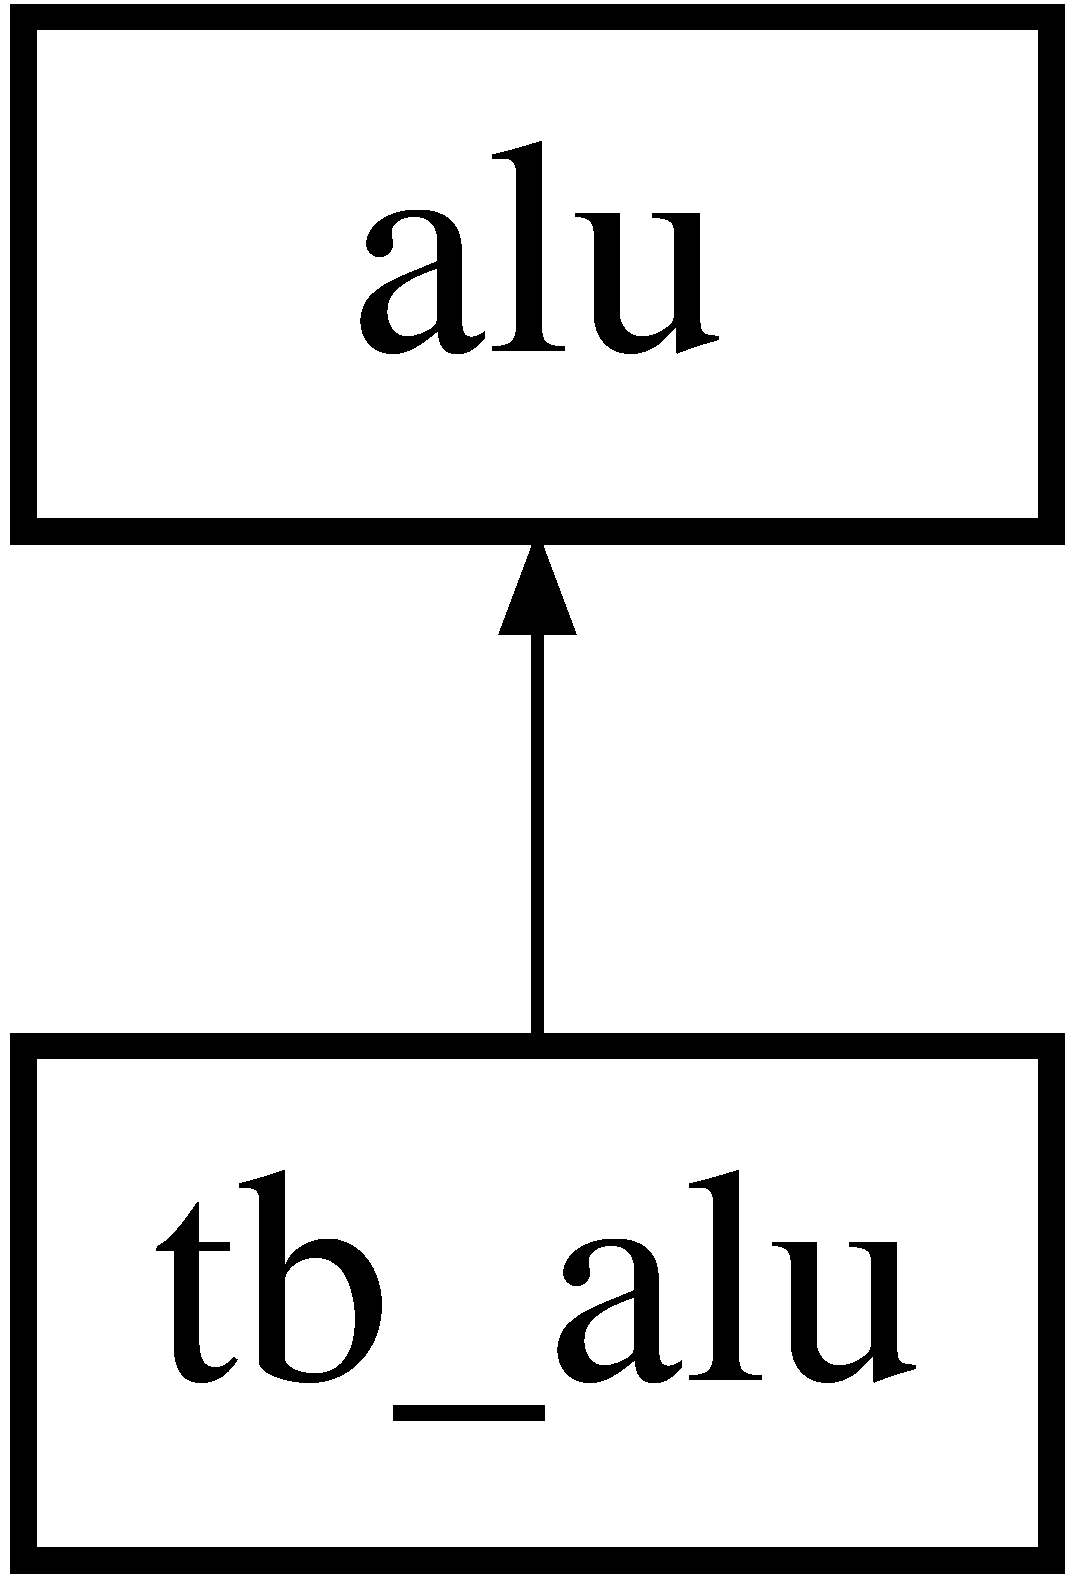
\includegraphics[height=2.000000cm]{classtb__alu}
\end{center}
\end{figure}
\subsection*{Entities}
\begin{DoxyCompactItemize}
\item 
\hyperlink{classtb__alu_1_1sim}{sim} architecture
\begin{DoxyCompactList}\small\item\em A\+LU Testbench Architecture S\+IM. \end{DoxyCompactList}\end{DoxyCompactItemize}
\subsection*{Libraries}
 \begin{DoxyCompactItemize}
\item 
\hyperlink{classtb__alu_ae4f03c286607f3181e16b9aa12d0c6d4}{I\+E\+EE} 
\end{DoxyCompactItemize}
\subsection*{Use Clauses}
 \begin{DoxyCompactItemize}
\item 
\hyperlink{classtb__alu_acd03516902501cd1c7296a98e22c6fcb}{std\+\_\+logic\+\_\+1164}   
\end{DoxyCompactItemize}


\subsection{Detailed Description}
A\+LU Testbench Entity. 

The Calculator Control unit is part of the calculator project. 

\subsection{Member Data Documentation}
\mbox{\Hypertarget{classtb__alu_ae4f03c286607f3181e16b9aa12d0c6d4}\label{classtb__alu_ae4f03c286607f3181e16b9aa12d0c6d4}} 
\index{tb\+\_\+alu@{tb\+\_\+alu}!I\+E\+EE@{I\+E\+EE}}
\index{I\+E\+EE@{I\+E\+EE}!tb\+\_\+alu@{tb\+\_\+alu}}
\subsubsection{\texorpdfstring{I\+E\+EE}{IEEE}}
{\footnotesize\ttfamily \hyperlink{classtb__alu_ae4f03c286607f3181e16b9aa12d0c6d4}{I\+E\+EE}\hspace{0.3cm}{\ttfamily [Library]}}

\mbox{\Hypertarget{classtb__alu_acd03516902501cd1c7296a98e22c6fcb}\label{classtb__alu_acd03516902501cd1c7296a98e22c6fcb}} 
\index{tb\+\_\+alu@{tb\+\_\+alu}!std\+\_\+logic\+\_\+1164@{std\+\_\+logic\+\_\+1164}}
\index{std\+\_\+logic\+\_\+1164@{std\+\_\+logic\+\_\+1164}!tb\+\_\+alu@{tb\+\_\+alu}}
\subsubsection{\texorpdfstring{std\+\_\+logic\+\_\+1164}{std\_logic\_1164}}
{\footnotesize\ttfamily \hyperlink{classtb__alu_acd03516902501cd1c7296a98e22c6fcb}{std\+\_\+logic\+\_\+1164}\hspace{0.3cm}{\ttfamily [Package]}}



The documentation for this class was generated from the following file\+:\begin{DoxyCompactItemize}
\item 
tb/\hyperlink{tb__alu___8vhd}{tb\+\_\+alu\+\_\+.\+vhd}\end{DoxyCompactItemize}

\hypertarget{classtb__calc__ctrl}{}\section{tb\+\_\+calc\+\_\+ctrl Entity Reference}
\label{classtb__calc__ctrl}\index{tb\+\_\+calc\+\_\+ctrl@{tb\+\_\+calc\+\_\+ctrl}}


Calculator Control Unit Testbench Entity.  


Inheritance diagram for tb\+\_\+calc\+\_\+ctrl\+:\begin{figure}[H]
\begin{center}
\leavevmode
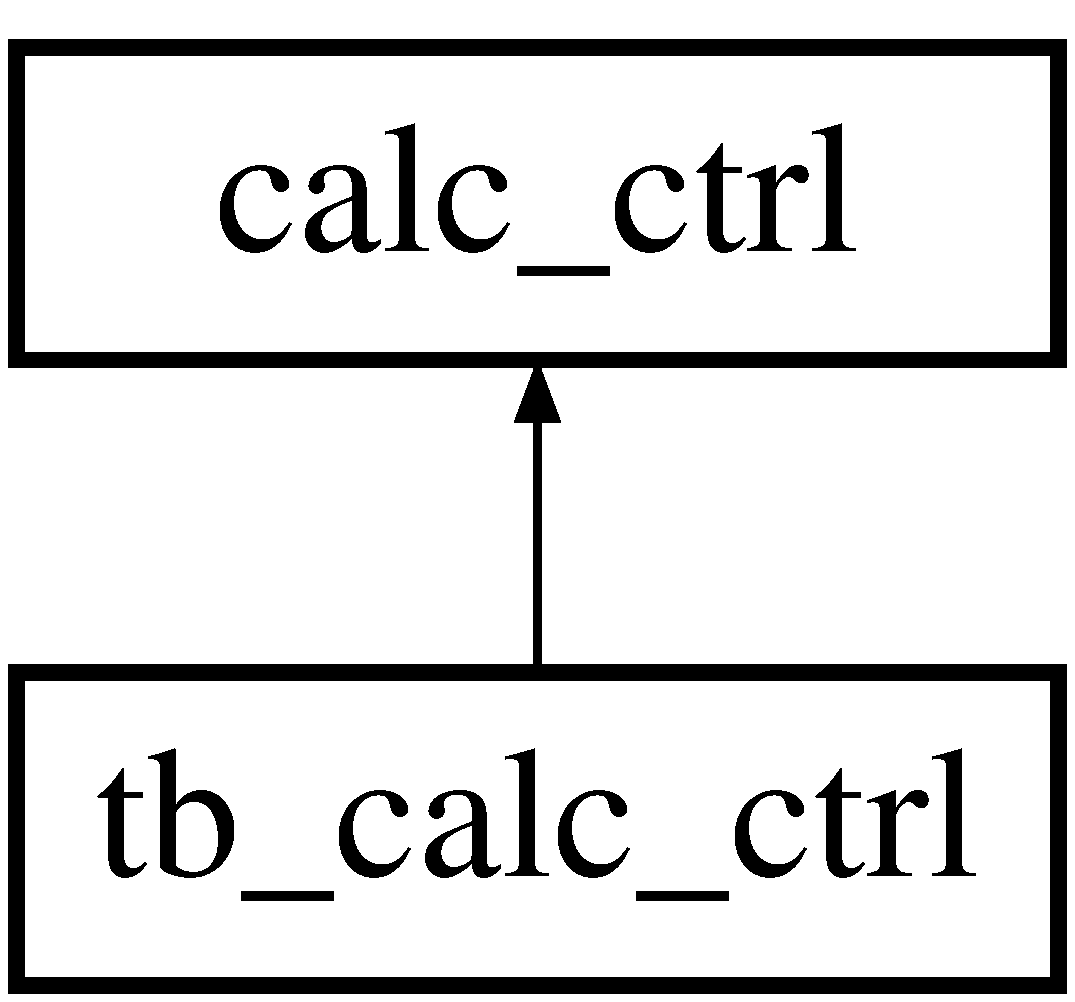
\includegraphics[height=2.000000cm]{classtb__calc__ctrl}
\end{center}
\end{figure}
\subsection*{Entities}
\begin{DoxyCompactItemize}
\item 
\hyperlink{classtb__calc__ctrl_1_1sim}{sim} architecture
\begin{DoxyCompactList}\small\item\em Calculcator Control Unit Testbench Architecture S\+IM. \end{DoxyCompactList}\end{DoxyCompactItemize}
\subsection*{Libraries}
 \begin{DoxyCompactItemize}
\item 
\hyperlink{classtb__calc__ctrl_ae4f03c286607f3181e16b9aa12d0c6d4}{I\+E\+EE} 
\end{DoxyCompactItemize}
\subsection*{Use Clauses}
 \begin{DoxyCompactItemize}
\item 
\hyperlink{classtb__calc__ctrl_acd03516902501cd1c7296a98e22c6fcb}{std\+\_\+logic\+\_\+1164}   
\end{DoxyCompactItemize}


\subsection{Detailed Description}
Calculator Control Unit Testbench Entity. 

The Calculator Control unit is part of the calculator project. 

\subsection{Member Data Documentation}
\mbox{\Hypertarget{classtb__calc__ctrl_ae4f03c286607f3181e16b9aa12d0c6d4}\label{classtb__calc__ctrl_ae4f03c286607f3181e16b9aa12d0c6d4}} 
\index{tb\+\_\+calc\+\_\+ctrl@{tb\+\_\+calc\+\_\+ctrl}!I\+E\+EE@{I\+E\+EE}}
\index{I\+E\+EE@{I\+E\+EE}!tb\+\_\+calc\+\_\+ctrl@{tb\+\_\+calc\+\_\+ctrl}}
\subsubsection{\texorpdfstring{I\+E\+EE}{IEEE}}
{\footnotesize\ttfamily \hyperlink{classtb__calc__ctrl_ae4f03c286607f3181e16b9aa12d0c6d4}{I\+E\+EE}\hspace{0.3cm}{\ttfamily [Library]}}

\mbox{\Hypertarget{classtb__calc__ctrl_acd03516902501cd1c7296a98e22c6fcb}\label{classtb__calc__ctrl_acd03516902501cd1c7296a98e22c6fcb}} 
\index{tb\+\_\+calc\+\_\+ctrl@{tb\+\_\+calc\+\_\+ctrl}!std\+\_\+logic\+\_\+1164@{std\+\_\+logic\+\_\+1164}}
\index{std\+\_\+logic\+\_\+1164@{std\+\_\+logic\+\_\+1164}!tb\+\_\+calc\+\_\+ctrl@{tb\+\_\+calc\+\_\+ctrl}}
\subsubsection{\texorpdfstring{std\+\_\+logic\+\_\+1164}{std\_logic\_1164}}
{\footnotesize\ttfamily \hyperlink{classtb__calc__ctrl_acd03516902501cd1c7296a98e22c6fcb}{std\+\_\+logic\+\_\+1164}\hspace{0.3cm}{\ttfamily [Package]}}



The documentation for this class was generated from the following file\+:\begin{DoxyCompactItemize}
\item 
tb/\hyperlink{tb__calc__ctrl___8vhd}{tb\+\_\+calc\+\_\+ctrl\+\_\+.\+vhd}\end{DoxyCompactItemize}

\hypertarget{classtb__calc__top}{}\section{tb\+\_\+calc\+\_\+top Entity Reference}
\label{classtb__calc__top}\index{tb\+\_\+calc\+\_\+top@{tb\+\_\+calc\+\_\+top}}


Calculator Top Design Testbench Entity.  


Inheritance diagram for tb\+\_\+calc\+\_\+top\+:\begin{figure}[H]
\begin{center}
\leavevmode
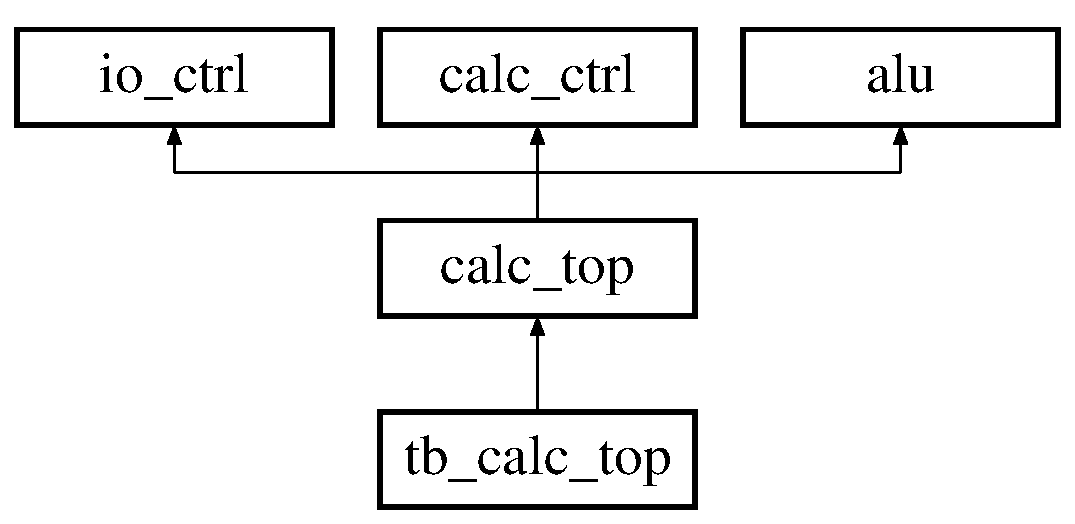
\includegraphics[height=3.000000cm]{classtb__calc__top}
\end{center}
\end{figure}
\subsection*{Entities}
\begin{DoxyCompactItemize}
\item 
\hyperlink{classtb__calc__top_1_1sim}{sim} architecture
\begin{DoxyCompactList}\small\item\em Calculator Top Design Testbench Architecture S\+IM. \end{DoxyCompactList}\end{DoxyCompactItemize}
\subsection*{Libraries}
 \begin{DoxyCompactItemize}
\item 
\hyperlink{classtb__calc__top_ae4f03c286607f3181e16b9aa12d0c6d4}{I\+E\+EE} 
\end{DoxyCompactItemize}
\subsection*{Use Clauses}
 \begin{DoxyCompactItemize}
\item 
\hyperlink{classtb__calc__top_acd03516902501cd1c7296a98e22c6fcb}{std\+\_\+logic\+\_\+1164}   
\end{DoxyCompactItemize}


\subsection{Detailed Description}
Calculator Top Design Testbench Entity. 

The Calculator Control unit is part of the calculator project. 

\subsection{Member Data Documentation}
\mbox{\Hypertarget{classtb__calc__top_ae4f03c286607f3181e16b9aa12d0c6d4}\label{classtb__calc__top_ae4f03c286607f3181e16b9aa12d0c6d4}} 
\index{tb\+\_\+calc\+\_\+top@{tb\+\_\+calc\+\_\+top}!I\+E\+EE@{I\+E\+EE}}
\index{I\+E\+EE@{I\+E\+EE}!tb\+\_\+calc\+\_\+top@{tb\+\_\+calc\+\_\+top}}
\subsubsection{\texorpdfstring{I\+E\+EE}{IEEE}}
{\footnotesize\ttfamily \hyperlink{classtb__calc__top_ae4f03c286607f3181e16b9aa12d0c6d4}{I\+E\+EE}\hspace{0.3cm}{\ttfamily [Library]}}

\mbox{\Hypertarget{classtb__calc__top_acd03516902501cd1c7296a98e22c6fcb}\label{classtb__calc__top_acd03516902501cd1c7296a98e22c6fcb}} 
\index{tb\+\_\+calc\+\_\+top@{tb\+\_\+calc\+\_\+top}!std\+\_\+logic\+\_\+1164@{std\+\_\+logic\+\_\+1164}}
\index{std\+\_\+logic\+\_\+1164@{std\+\_\+logic\+\_\+1164}!tb\+\_\+calc\+\_\+top@{tb\+\_\+calc\+\_\+top}}
\subsubsection{\texorpdfstring{std\+\_\+logic\+\_\+1164}{std\_logic\_1164}}
{\footnotesize\ttfamily \hyperlink{classtb__calc__top_acd03516902501cd1c7296a98e22c6fcb}{std\+\_\+logic\+\_\+1164}\hspace{0.3cm}{\ttfamily [Package]}}



The documentation for this class was generated from the following file\+:\begin{DoxyCompactItemize}
\item 
tb/\hyperlink{tb__calc__top___8vhd}{tb\+\_\+calc\+\_\+top\+\_\+.\+vhd}\end{DoxyCompactItemize}

\hypertarget{classtb__io__ctrl}{}\section{tb\+\_\+io\+\_\+ctrl Entity Reference}
\label{classtb__io__ctrl}\index{tb\+\_\+io\+\_\+ctrl@{tb\+\_\+io\+\_\+ctrl}}


IO Control Unit Testbench Entity.  


Inheritance diagram for tb\+\_\+io\+\_\+ctrl\+:\begin{figure}[H]
\begin{center}
\leavevmode
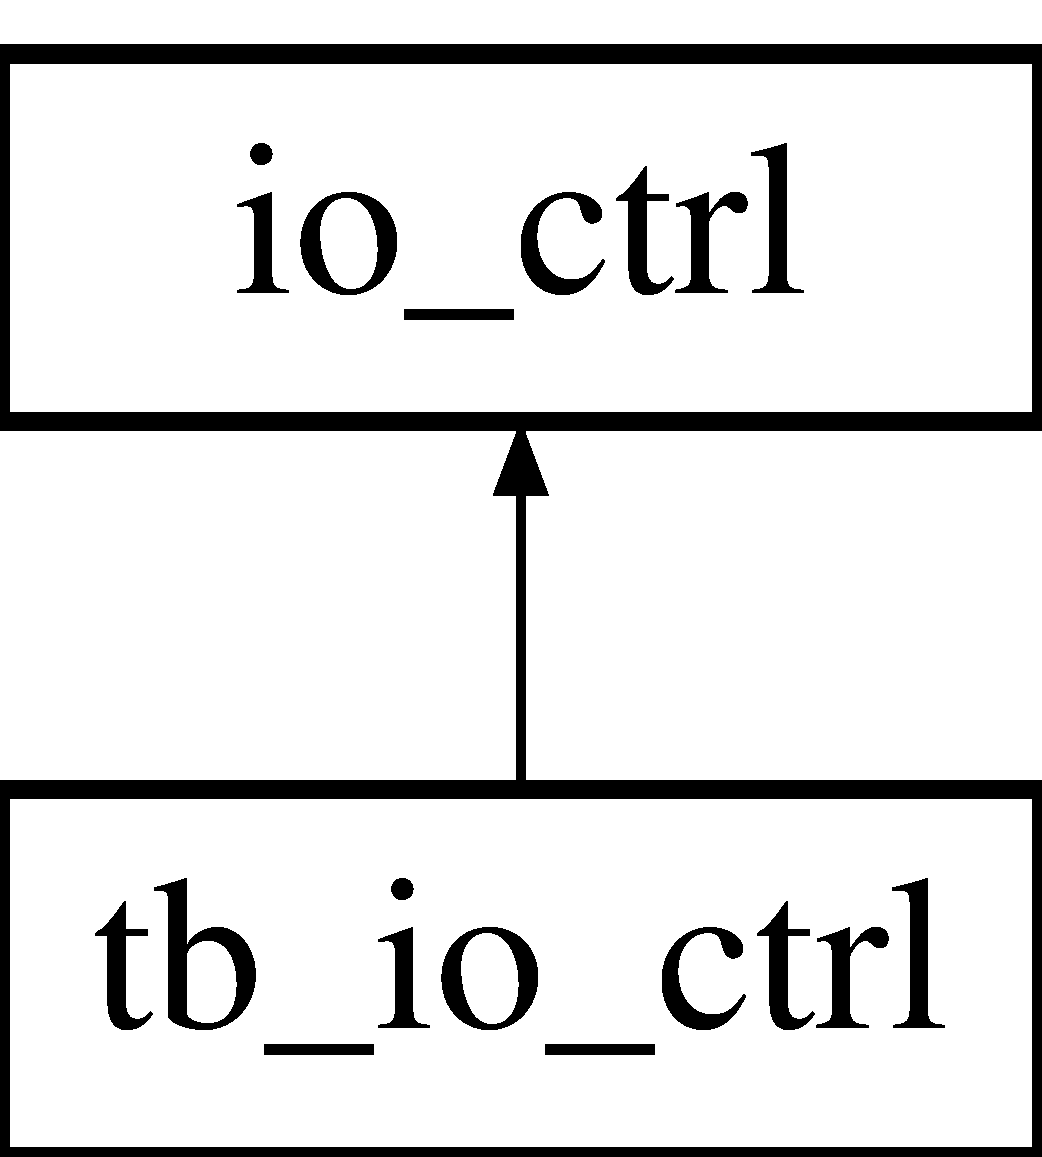
\includegraphics[height=2.000000cm]{classtb__io__ctrl}
\end{center}
\end{figure}
\subsection*{Entities}
\begin{DoxyCompactItemize}
\item 
\hyperlink{classtb__io__ctrl_1_1sim}{sim} architecture
\begin{DoxyCompactList}\small\item\em IO Control Unit Testbench Architecture. \end{DoxyCompactList}\end{DoxyCompactItemize}
\subsection*{Libraries}
 \begin{DoxyCompactItemize}
\item 
\mbox{\Hypertarget{classtb__io__ctrl_ae4f03c286607f3181e16b9aa12d0c6d4}\label{classtb__io__ctrl_ae4f03c286607f3181e16b9aa12d0c6d4}} 
\hyperlink{classtb__io__ctrl_ae4f03c286607f3181e16b9aa12d0c6d4}{I\+E\+EE} 
\end{DoxyCompactItemize}
\subsection*{Use Clauses}
 \begin{DoxyCompactItemize}
\item 
\mbox{\Hypertarget{classtb__io__ctrl_acd03516902501cd1c7296a98e22c6fcb}\label{classtb__io__ctrl_acd03516902501cd1c7296a98e22c6fcb}} 
\hyperlink{classtb__io__ctrl_acd03516902501cd1c7296a98e22c6fcb}{std\+\_\+logic\+\_\+1164}   
\end{DoxyCompactItemize}


\subsection{Detailed Description}
IO Control Unit Testbench Entity. 

The IO Control uniti part of the calculator project. 

The documentation for this class was generated from the following file\+:\begin{DoxyCompactItemize}
\item 
tb/\hyperlink{tb__io__ctrl___8vhd}{tb\+\_\+io\+\_\+ctrl\+\_\+.\+vhd}\end{DoxyCompactItemize}

\chapter{File Documentation}
\hypertarget{impl__1_2calc__top_8tcl}{}\section{impl/calculator.runs/impl\+\_\+1/calc\+\_\+top.tcl File Reference}
\label{impl__1_2calc__top_8tcl}\index{impl/calculator.\+runs/impl\+\_\+1/calc\+\_\+top.\+tcl@{impl/calculator.\+runs/impl\+\_\+1/calc\+\_\+top.\+tcl}}


\subsection{Function Documentation}
\mbox{\Hypertarget{impl__1_2calc__top_8tcl_af7a4bca0293e32dc65781e829a143793}\label{impl__1_2calc__top_8tcl_af7a4bca0293e32dc65781e829a143793}} 
\index{impl\+\_\+1/calc\+\_\+top.\+tcl@{impl\+\_\+1/calc\+\_\+top.\+tcl}!end\+\_\+step@{end\+\_\+step}}
\index{end\+\_\+step@{end\+\_\+step}!impl\+\_\+1/calc\+\_\+top.\+tcl@{impl\+\_\+1/calc\+\_\+top.\+tcl}}
\subsubsection{\texorpdfstring{end\+\_\+step()}{end\_step()}}
{\footnotesize\ttfamily end\+\_\+step\begin{DoxyParamCaption}\item[{}]{step  }\end{DoxyParamCaption}}

\mbox{\Hypertarget{impl__1_2calc__top_8tcl_a1aa28d02a8b952c855b601dc2714e125}\label{impl__1_2calc__top_8tcl_a1aa28d02a8b952c855b601dc2714e125}} 
\index{impl\+\_\+1/calc\+\_\+top.\+tcl@{impl\+\_\+1/calc\+\_\+top.\+tcl}!start\+\_\+step@{start\+\_\+step}}
\index{start\+\_\+step@{start\+\_\+step}!impl\+\_\+1/calc\+\_\+top.\+tcl@{impl\+\_\+1/calc\+\_\+top.\+tcl}}
\subsubsection{\texorpdfstring{start\+\_\+step()}{start\_step()}}
{\footnotesize\ttfamily start\+\_\+step\begin{DoxyParamCaption}\item[{}]{step  }\end{DoxyParamCaption}}

\mbox{\Hypertarget{impl__1_2calc__top_8tcl_a935d6826d74027ee5d88b324def30f2c}\label{impl__1_2calc__top_8tcl_a935d6826d74027ee5d88b324def30f2c}} 
\index{impl\+\_\+1/calc\+\_\+top.\+tcl@{impl\+\_\+1/calc\+\_\+top.\+tcl}!step\+\_\+failed@{step\+\_\+failed}}
\index{step\+\_\+failed@{step\+\_\+failed}!impl\+\_\+1/calc\+\_\+top.\+tcl@{impl\+\_\+1/calc\+\_\+top.\+tcl}}
\subsubsection{\texorpdfstring{step\+\_\+failed()}{step\_failed()}}
{\footnotesize\ttfamily step\+\_\+failed\begin{DoxyParamCaption}\item[{}]{step  }\end{DoxyParamCaption}}


\hypertarget{synth__1_2calc__top_8tcl}{}\section{impl/calculator.runs/synth\+\_\+1/calc\+\_\+top.tcl File Reference}
\label{synth__1_2calc__top_8tcl}\index{impl/calculator.\+runs/synth\+\_\+1/calc\+\_\+top.\+tcl@{impl/calculator.\+runs/synth\+\_\+1/calc\+\_\+top.\+tcl}}

\hypertarget{_r_e_a_d_m_e_8md}{}\section{R\+E\+A\+D\+M\+E.\+md File Reference}
\label{_r_e_a_d_m_e_8md}\index{R\+E\+A\+D\+M\+E.\+md@{R\+E\+A\+D\+M\+E.\+md}}

\hypertarget{tb__alu___8vhd}{}\section{tb/tb\+\_\+alu\+\_\+.vhd File Reference}
\label{tb__alu___8vhd}\index{tb/tb\+\_\+alu\+\_\+.\+vhd@{tb/tb\+\_\+alu\+\_\+.\+vhd}}


A\+LU Testbench Entity.  


\subsection*{Entities}
\begin{DoxyCompactItemize}
\item 
\hyperlink{classtb__alu}{tb\+\_\+alu} entity
\begin{DoxyCompactList}\small\item\em A\+LU Testbench Entity. \end{DoxyCompactList}\end{DoxyCompactItemize}


\subsection{Detailed Description}
A\+LU Testbench Entity. 


\hypertarget{tb__alu__sim_8vhd}{}\section{tb/tb\+\_\+alu\+\_\+sim.vhd File Reference}
\label{tb__alu__sim_8vhd}\index{tb/tb\+\_\+alu\+\_\+sim.\+vhd@{tb/tb\+\_\+alu\+\_\+sim.\+vhd}}


A\+LU Testbench Architecture S\+IM.  


\subsection*{Entities}
\begin{DoxyCompactItemize}
\item 
\hyperlink{classtb__alu_1_1sim}{sim} architecture
\begin{DoxyCompactList}\small\item\em A\+LU Testbench Architecture S\+IM. \end{DoxyCompactList}\end{DoxyCompactItemize}


\subsection{Detailed Description}
A\+LU Testbench Architecture S\+IM. 


\hypertarget{tb__calc__ctrl___8vhd}{}\section{tb/tb\+\_\+calc\+\_\+ctrl\+\_\+.vhd File Reference}
\label{tb__calc__ctrl___8vhd}\index{tb/tb\+\_\+calc\+\_\+ctrl\+\_\+.\+vhd@{tb/tb\+\_\+calc\+\_\+ctrl\+\_\+.\+vhd}}


Calculator Control Unit Testbench Entity.  


\subsection*{Entities}
\begin{DoxyCompactItemize}
\item 
\hyperlink{classtb__calc__ctrl}{tb\+\_\+calc\+\_\+ctrl} entity
\begin{DoxyCompactList}\small\item\em Calculator Control Unit Testbench Entity. \end{DoxyCompactList}\end{DoxyCompactItemize}


\subsection{Detailed Description}
Calculator Control Unit Testbench Entity. 


\hypertarget{tb__calc__ctrl__sim_8vhd}{}\section{tb/tb\+\_\+calc\+\_\+ctrl\+\_\+sim.vhd File Reference}
\label{tb__calc__ctrl__sim_8vhd}\index{tb/tb\+\_\+calc\+\_\+ctrl\+\_\+sim.\+vhd@{tb/tb\+\_\+calc\+\_\+ctrl\+\_\+sim.\+vhd}}


Calculcator Control Unit Testbench Architecture S\+IM.  


\subsection*{Entities}
\begin{DoxyCompactItemize}
\item 
\hyperlink{classtb__calc__ctrl_1_1sim}{sim} architecture
\begin{DoxyCompactList}\small\item\em Calculcator Control Unit Testbench Architecture S\+IM. \end{DoxyCompactList}\end{DoxyCompactItemize}


\subsection{Detailed Description}
Calculcator Control Unit Testbench Architecture S\+IM. 


\hypertarget{tb__calc__top___8vhd}{}\section{tb/tb\+\_\+calc\+\_\+top\+\_\+.vhd File Reference}
\label{tb__calc__top___8vhd}\index{tb/tb\+\_\+calc\+\_\+top\+\_\+.\+vhd@{tb/tb\+\_\+calc\+\_\+top\+\_\+.\+vhd}}


Calculator Top Design Testbench Entity.  


\subsection*{Entities}
\begin{DoxyCompactItemize}
\item 
\hyperlink{classtb__calc__top}{tb\+\_\+calc\+\_\+top} entity
\begin{DoxyCompactList}\small\item\em Calculator Top Design Testbench Entity. \end{DoxyCompactList}\end{DoxyCompactItemize}


\subsection{Detailed Description}
Calculator Top Design Testbench Entity. 


\hypertarget{tb__calc__top__sim_8vhd}{}\section{tb/tb\+\_\+calc\+\_\+top\+\_\+sim.vhd File Reference}
\label{tb__calc__top__sim_8vhd}\index{tb/tb\+\_\+calc\+\_\+top\+\_\+sim.\+vhd@{tb/tb\+\_\+calc\+\_\+top\+\_\+sim.\+vhd}}


Calculator Top Design Testbench Architecture S\+IM.  


\subsection*{Entities}
\begin{DoxyCompactItemize}
\item 
\hyperlink{classtb__calc__top_1_1sim}{sim} architecture
\begin{DoxyCompactList}\small\item\em Calculator Top Design Testbench Architecture S\+IM. \end{DoxyCompactList}\end{DoxyCompactItemize}


\subsection{Detailed Description}
Calculator Top Design Testbench Architecture S\+IM. 


\hypertarget{tb__io__ctrl___8vhd}{}\section{tb/tb\+\_\+io\+\_\+ctrl\+\_\+.vhd File Reference}
\label{tb__io__ctrl___8vhd}\index{tb/tb\+\_\+io\+\_\+ctrl\+\_\+.\+vhd@{tb/tb\+\_\+io\+\_\+ctrl\+\_\+.\+vhd}}


IO Control Unit Testbench Entity.  


\subsection*{Entities}
\begin{DoxyCompactItemize}
\item 
\hyperlink{classtb__io__ctrl}{tb\+\_\+io\+\_\+ctrl} entity
\begin{DoxyCompactList}\small\item\em IO Control Unit Testbench Entity. \end{DoxyCompactList}\end{DoxyCompactItemize}


\subsection{Detailed Description}
IO Control Unit Testbench Entity. 


\hypertarget{tb__io__ctrl__sim_8vhd}{}\section{tb/tb\+\_\+io\+\_\+ctrl\+\_\+sim.vhd File Reference}
\label{tb__io__ctrl__sim_8vhd}\index{tb/tb\+\_\+io\+\_\+ctrl\+\_\+sim.\+vhd@{tb/tb\+\_\+io\+\_\+ctrl\+\_\+sim.\+vhd}}


IO Control Unit Testbench Architecture S\+IM.  


\subsection*{Entities}
\begin{DoxyCompactItemize}
\item 
\hyperlink{classtb__io__ctrl_1_1sim}{sim} architecture
\begin{DoxyCompactList}\small\item\em IO Control Unit Testbench Architecture S\+IM. \end{DoxyCompactList}\end{DoxyCompactItemize}


\subsection{Detailed Description}
IO Control Unit Testbench Architecture S\+IM. 


\hypertarget{alu___8vhd}{}\section{vhdl/alu\+\_\+.vhd File Reference}
\label{alu___8vhd}\index{vhdl/alu\+\_\+.\+vhd@{vhdl/alu\+\_\+.\+vhd}}


A\+LU Entity.  


\subsection*{Entities}
\begin{DoxyCompactItemize}
\item 
\hyperlink{classalu}{alu} entity
\begin{DoxyCompactList}\small\item\em A\+LU Entity. \end{DoxyCompactList}\end{DoxyCompactItemize}


\subsection{Detailed Description}
A\+LU Entity. 


\hypertarget{alu__rtl_8vhd}{}\section{vhdl/alu\+\_\+rtl.vhd File Reference}
\label{alu__rtl_8vhd}\index{vhdl/alu\+\_\+rtl.\+vhd@{vhdl/alu\+\_\+rtl.\+vhd}}


A\+LU Architecture R\+TL.  


\subsection*{Entities}
\begin{DoxyCompactItemize}
\item 
\hyperlink{classalu_1_1rtl}{rtl} architecture
\begin{DoxyCompactList}\small\item\em A\+LU Architecture R\+TL. \end{DoxyCompactList}\end{DoxyCompactItemize}


\subsection{Detailed Description}
A\+LU Architecture R\+TL. 


\hypertarget{calc__ctrl___8vhd}{}\section{vhdl/calc\+\_\+ctrl\+\_\+.vhd File Reference}
\label{calc__ctrl___8vhd}\index{vhdl/calc\+\_\+ctrl\+\_\+.\+vhd@{vhdl/calc\+\_\+ctrl\+\_\+.\+vhd}}


Calculator Control Unit Entity.  


\subsection*{Entities}
\begin{DoxyCompactItemize}
\item 
\hyperlink{classcalc__ctrl}{calc\+\_\+ctrl} entity
\begin{DoxyCompactList}\small\item\em Calculator Control Unit Entity. \end{DoxyCompactList}\end{DoxyCompactItemize}


\subsection{Detailed Description}
Calculator Control Unit Entity. 


\hypertarget{calc__ctrl__rtl_8vhd}{}\section{vhdl/calc\+\_\+ctrl\+\_\+rtl.vhd File Reference}
\label{calc__ctrl__rtl_8vhd}\index{vhdl/calc\+\_\+ctrl\+\_\+rtl.\+vhd@{vhdl/calc\+\_\+ctrl\+\_\+rtl.\+vhd}}


Calculator Control Unit Architecture R\+TL.  


\subsection*{Entities}
\begin{DoxyCompactItemize}
\item 
\hyperlink{classcalc__ctrl_1_1rtl}{rtl} architecture
\begin{DoxyCompactList}\small\item\em Calclator Control Unit Architecture R\+TL. \end{DoxyCompactList}\end{DoxyCompactItemize}


\subsection{Detailed Description}
Calculator Control Unit Architecture R\+TL. 


\hypertarget{calc__top___8vhd}{}\section{vhdl/calc\+\_\+top\+\_\+.vhd File Reference}
\label{calc__top___8vhd}\index{vhdl/calc\+\_\+top\+\_\+.\+vhd@{vhdl/calc\+\_\+top\+\_\+.\+vhd}}


Calculator Top Design Entity.  


\subsection*{Entities}
\begin{DoxyCompactItemize}
\item 
\hyperlink{classcalc__top}{calc\+\_\+top} entity
\begin{DoxyCompactList}\small\item\em Calculator Top Design Entity. \end{DoxyCompactList}\end{DoxyCompactItemize}


\subsection{Detailed Description}
Calculator Top Design Entity. 


\hypertarget{calc__top__rtl_8vhd}{}\section{vhdl/calc\+\_\+top\+\_\+rtl.vhd File Reference}
\label{calc__top__rtl_8vhd}\index{vhdl/calc\+\_\+top\+\_\+rtl.\+vhd@{vhdl/calc\+\_\+top\+\_\+rtl.\+vhd}}


Calculator Top Architecture R\+T\+L-\/\+S\+T\+R\+UC.  


\subsection*{Entities}
\begin{DoxyCompactItemize}
\item 
\hyperlink{classcalc__top_1_1struc}{struc} architecture
\begin{DoxyCompactList}\small\item\em Calculator Top Architecture R\+T\+L-\/\+S\+T\+R\+UC. \end{DoxyCompactList}\end{DoxyCompactItemize}


\subsection{Detailed Description}
Calculator Top Architecture R\+T\+L-\/\+S\+T\+R\+UC. 


\hypertarget{io__ctrl___8vhd}{}\section{vhdl/io\+\_\+ctrl\+\_\+.vhd File Reference}
\label{io__ctrl___8vhd}\index{vhdl/io\+\_\+ctrl\+\_\+.\+vhd@{vhdl/io\+\_\+ctrl\+\_\+.\+vhd}}


IO Control Unit Entity.  


\subsection*{Entities}
\begin{DoxyCompactItemize}
\item 
\hyperlink{classio__ctrl}{io\+\_\+ctrl} entity
\begin{DoxyCompactList}\small\item\em IO Control Unit Entity. \end{DoxyCompactList}\end{DoxyCompactItemize}


\subsection{Detailed Description}
IO Control Unit Entity. 


\hypertarget{io__ctrl__rtl_8vhd}{}\section{vhdl/io\+\_\+ctrl\+\_\+rtl.vhd File Reference}
\label{io__ctrl__rtl_8vhd}\index{vhdl/io\+\_\+ctrl\+\_\+rtl.\+vhd@{vhdl/io\+\_\+ctrl\+\_\+rtl.\+vhd}}


IO Control Unit Architecture.  


\subsection*{Entities}
\begin{DoxyCompactItemize}
\item 
\hyperlink{classio__ctrl_1_1rtl}{rtl} architecture
\begin{DoxyCompactList}\small\item\em IO Control Unit Architecture. \end{DoxyCompactList}\end{DoxyCompactItemize}


\subsection{Detailed Description}
IO Control Unit Architecture. 


%--- End generated contents ---

% Index
\backmatter
\newpage
\phantomsection
\clearemptydoublepage
\addcontentsline{toc}{chapter}{Index}
\printindex

\end{document}
